\documentclass{beamer}
\usepackage[T1]{fontenc}
\usepackage[utf8]{inputenc}
\usepackage{lmodern}
\usepackage[english]{babel}

\usepackage{verbatim}
\usepackage{mathtools}
\usepackage{stmaryrd}


\usepackage{geometry}
\usepackage{setspace}

\usepackage{latex/agda}
\usepackage{unicode-math}
\setmathfont{XITS Math}

\usepackage{newunicodechar}
\newunicodechar{→}{\ensuremath{\mathnormal\to}}
% \newunicodechar{ℕ}{\ensuremath{\mathnormal\bN}}
\newunicodechar{ℓ}{\ensuremath{\mathnormal\ell}}
\newunicodechar{↪}{\ensuremath{\mathnormal\hookrightarrow}}
\newunicodechar{⟶}{\ensuremath{\mathnormal\hookrightarrow}}
\newunicodechar{𝑀}{$M$}

% \newunicodechar{ℕ}{$\mathbb{N}$}
\newunicodechar{⊨}{\ensuremath{\vDash}}
\newunicodechar{⊧}{$\models$}

\newunicodechar{ℕ}{$N$}
\newunicodechar{ϕ}{$\phi$}
\newunicodechar{∨}{$\lor$}
\newunicodechar{∧}{$\land$}
\newunicodechar{⇒}{$\Rightarrow$}
\newunicodechar{π}{$\pi$}
\newunicodechar{ψ}{$\psi$}
\newunicodechar{Σ}{$\Sigma$}
\newunicodechar{∈}{$\in$}
\newunicodechar{∀}{$\forall$}
\newunicodechar{≤}{$\leq$}
\newunicodechar{⊎}{$\uplus$}
\newunicodechar{≡}{$\equiv$}
\newunicodechar{∷}{$::$}

%πψ

\newunicodechar{⊥}{$\bot$}
\newunicodechar{⊤}{$\top$}
% ⊥ ⊤
  % _∨_ _∧_ _⇒_ : → ϕ → ϕ


\usepackage{xcolor}
\usepackage[normalem]{ulem}%per barrare parole
\usepackage{soul} %barrare numeri
% \usepackage{booktabs}%per tabelle
\usepackage{amsmath} %leqno mette elenchi in align a sx
\usepackage{amssymb}
% \usepackage{enumitem} %personalizza gli elenchi
% \usepackage{amsthm} %teoremi e definizioni
\usepackage{tikz-cd}
% \tikzcdset{scale cd/.style={every label/.append style={scale=#1} }}
\tikzcdset{scale cd/.style={every label/.append style={scale=#1}, cells={nodes={scale=#1}}}}

\usepackage{multirow}%più righe nella stessa cella in tabella
\usepackage{multicol}
\usepackage{caption}
\usepackage{bussproofs}
\usepackage{soul}
\newcommand{\mathcolorbox}[2]{\colorbox{#1}{$\displaystyle #2$}}

\usetheme{Antibes}
\usecolortheme{beaver}
\useinnertheme{rounded}
\useoutertheme{infolines}

\titlegraphic{
  
\includegraphics[width=25mm]{pics/hw.png}
  
\includegraphics[width=25mm]{pics/aisec.png}
  
\includegraphics[width=25mm]{pics/laiv.png}}
\title{On the syntax and semantics of voice assistants in autonomous vehicles}
\author{Warrick Macmillan}
\date{$6^{th}$ May 2022}



\begin{document}

\begin{frame}
  \titlepage
\end{frame}

\section{Overview}


% \subsection{Quick Recapitulation}

\begin{frame}
\frametitle{Motivation}

\begin{exampleblock}{}

  ``Go to the grocery store after the next exit, and then go to fuel station,
but stop by the fire hydrant so I can take a picture of that crazy sign,
first.''

\end{exampleblock}
\pause
\begin{figure}
\hspace*{-3mm}%
\centering
   \pause
   
\includegraphics[width=1.5cm]{pics/hydrant.png}
   \pause
   
\includegraphics[width=3cm]{pics/crazy.jpg}
   % 
\includegraphics[width=2cm]{pics/exit.jpg}
   % 
\includegraphics[width=3cm]{pics/shop.jpeg}
\end{figure}
\pause
\begin{figure}
\hspace*{-3mm}%
\centering
   % 
\includegraphics[width=1.5cm]{pics/hydrant.png}
   % 
\includegraphics[width=3cm]{pics/crazy.jpg}
   
\includegraphics[width=2cm]{pics/exit.jpg}
   \pause
   
\includegraphics[width=3cm]{pics/shop.jpeg}
   \pause
   
\includegraphics[width=3cm]{pics/charge.jpg}
\end{figure}
  
\end{frame}

\begin{frame}
\frametitle{Ambiguities}

\begin{center}
\begin{minipage}{4cm}
\begin{alertblock}{}
``Go into the other lane''
\end{alertblock}
\end{minipage}
\end{center}
\pause
\begin{figure}
\hspace*{-3mm}%
\centering
    % \includegraphics[width=4cm,angle=45]{Ques}
    % \includegraphics[angle=45,width=4cm]{Ques}
   
\includegraphics[width=4cm]{pics/singleLane.jpg}
   \pause
   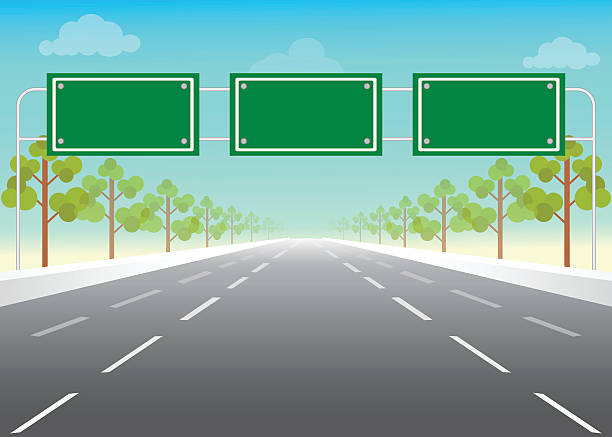
\includegraphics[width=6cm]{pics/multipleLane.jpg}
\end{figure}
  
\end{frame}

\begin{frame}

\frametitle{Ambiguities (cont.)}

\begin{center}
\begin{minipage}{6cm}
\begin{alertblock}{}
``Drive to the person with the dog''
\end{alertblock}
\end{minipage}
\end{center}

\pause
\begin{figure}
\hspace*{-3mm}%
\centering
   
\includegraphics[width=5cm]{pics/personDog.png}
   \pause
   
\includegraphics[width=5cm]{pics/dogCar.png}
\end{figure}
  
\end{frame}

\begin{frame}
\frametitle{Simplified Autonomous Vehicle}
\begin{figure}
\centering
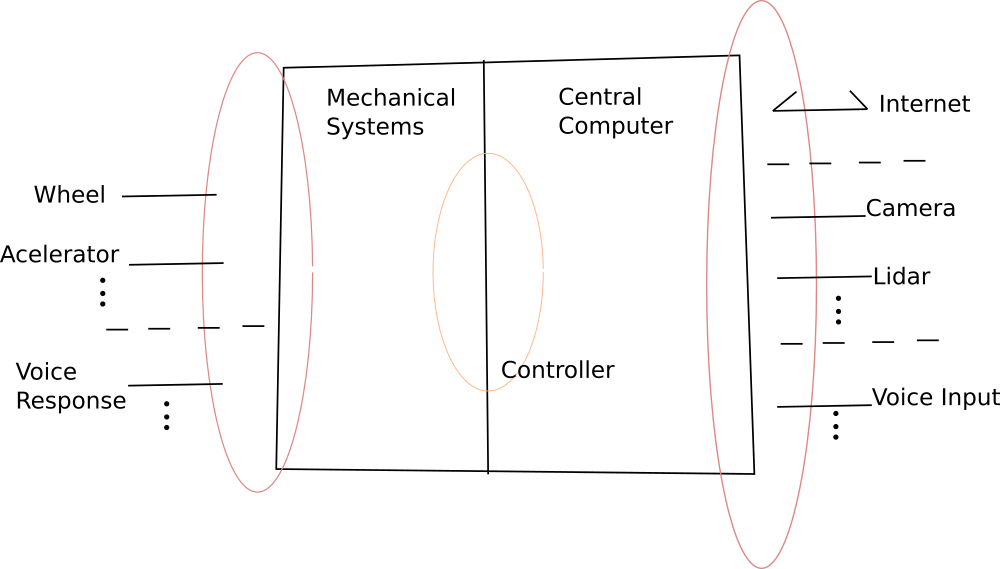
\includegraphics[width=100mm]{pics/selfDriving.png}
\caption{Self-driving car}\label{fig:A1}
\end{figure}

\end{frame}

\begin{frame}
\frametitle{Path}
\begin{figure}
\centering
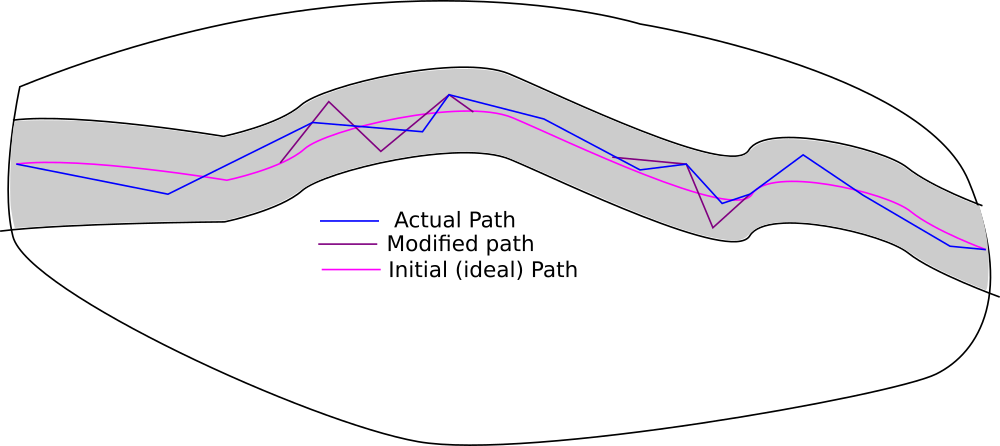
\includegraphics[width=100mm]{pics/diagramTrial1.png}
\caption{Initial, modified, and actual paths/routes}\label{fig:A2}
\end{figure}

\end{frame}

\begin{frame}
\begin{block}{Mathematically Ideal Property}
  $\forall u \in \text{Utt}.\; \exists r \in \text{Routes}$
  such that $\forall r' \in \text{Routes}.\; d(u,r) \leq d(u,r')$
\end{block}
\pause
\begin{exampleblock}{}
where $d$ is some hypothetical metric which should depend on
\pause
\begin{itemize}[<+->]
\item Cost
\item Safety
\item Legality
\item Adversaries
\end{itemize}
\end{exampleblock}
\pause
\begin{exampleblock}{}
and where
\pause
\begin{itemize}[<+->]
\item The set of utterances is a set of strings over a standard alphabet
\item The set of routes is some discretized set of paths in Euclidean 2-space
\end{itemize}
\pause
subject to constraints on the sets imposed by, for example
\pause
\begin{itemize}[<+->]
\item grammars in the case of strings
\item physical objects in the case of paths in Euclidean space
\end{itemize}
\end{exampleblock}



% \begin{itemize}
% \item Functional Programming languages : GF (Grammatical Framework), Haskell, Theorem Provers (Agda, Coq, ...)
% \item Verification for Robotics Systems :  Temporal logic (mostly at the syntactic level, for now)
% \item Natural Language Processing : Semantic Parsing, Controlled Natural Languages
% \end{enumerate}



\end{frame}


\begin{frame}[fragile]
\frametitle{Verification Spectrum}
\begin{figure}
\centering

% https://tikzcd.yichuanshen.de/#N4Igdg9gJgpgziAXAbVABwnAlgFyxMJZABgBpiBdUkANwEMAbAVxiRAB12cYAPHYAMpYwAcwYwABAFEedALZpxAXxBLS6TLnyEUZAIxVajFm1XqQGbHgJEA7KQPV6zVohBmNV7UQBM5Q84mbpzcfIIwOBIQAGbSsgricCpqnlo2KAAs-k7GrhxcvPxCouISAAoAThBoMBU4AJ7J5pZpOsgAbNlGLmwhhcAAshF0aFU1dY0eFprWbWQ+Abm9BWEAqmC4EgAq8DhNqbO+pAs5PcEr-JXVtQ0AtABGdHAwUNu7+9Ne6chZJ91B+VC-AG0BgDAkAGEABYwADGAGthCIPi1DihOn9Ank+mEAJJgbgVOiwvA0SRbGEQCowOTlKpkioombeFB6Y6LM7uFKfVpHADMHIBU1RLOQfPZpyF3JF3yyAsleWFzO+AFYJf9FdLlW1OvKNaYtV82myMoLNc1tUQABykU0Kg2GF4ieBEUDRKpyJBskA4CBIHzc90QT2IPRkH1+0N6QMer1+CNevkx4NerIJ0Mq5MhvSddN6ewgBh0e5gsqWtzCbCwED285A4AAMSYYBJ2kYdIgIiJcjkSIkAihWGie1UFCUQA
% https://tikzcd.yichuanshen.de/#N4Igdg9gJgpgziAXAbVABwnAlgFyxMJZABgBpiBdUkANwEMAbAVxiRAB12cYAPHYAMpYwAcwYwAvp2lde-AKI86AWzTiJICaXSZc+QigCM5KrUYs2nbn0EwcUmbJsQAZg5nWFS1eLgatOth4BEQATCbU9MysiBxO-EKi6o7xwAAKAE4QaDAZOACe-togGEH6RADMEWbRlqkAsnZ0aFk5eYWaxaV6IShkhqZRFrGdgT0GyFUDkeYxIJqmMFAi8ESgLlnKSAAs1DgQSACsEhQSQA
\begin{tikzcd}
\substack{\text{Single}\\\text{Example}} & \substack{\text{Set}\\\text{of}\\\text{Examples}} & \substack{\text{Single}\\\text{Property}} & \substack{\text{Metaproperty}} \\
{} \arrow[rrr, "\text{Verifiability}" description] &                                        &                                & {}                  &    \\
\substack{\text{Unit}\\\text{Testing}} & \substack{\text{Property-based}\\\text{Testing}} & \substack{\text{Model}\\\text{Checking}} & \substack{\text{ITP}} \\

{} \arrow[rd, "FP" description]                    &                                        &                                &                     &    \\
                                                   & {} \arrow[rrr]                         &                                &                     & {}
               
\end{tikzcd}
\end{figure}

\end{frame}

% general
\begin{frame}
\frametitle{Main Idea}

\begin{itemize}[<+->]
\item Functional Programming is all about composition of higher order functions
\item Break down system into composable \emph{big-components}, each of which
\begin{itemize}[<+->]
\item admits composition of \emph{small-components}
\item operates under different verification conditions
\end{itemize}
\item Ensure maps between big-components are functorial with respect to
  small-component composition
\item Verification of system is can similarly be broken into sub-verifications
\end{itemize}
\end{frame}


% more specifically
\begin{frame}
\begin{exampleblock}{More Specifically}
This project contains bits and pieces of :
\end{exampleblock}
\pause
\begin{enumerate}[<+->]
\item Functional Programming Languages : GF (Grammatical Framework), Haskell, Agda
\item Natural Language Processing : Semantic Parsing, Controlled Natural Languages
\item Tools : Grammars and logical implementations for motion planning and verification
\end{enumerate}
\end{frame}


\begin{frame}
\frametitle{Ideal Pipeline}

\begin{equation} % \label{eq1}
\begin{split}
\text{Utterance} & \mathcolorbox{yellow}{\xrightarrow{\mathit{Speech\ Recognizer}}} \text{String}\\
 & \mathcolorbox{yellow}{\xrightarrow{\mathit{Canonicalization_{LLM}}}} \text{String}\\
 & \xrightarrow{\mathit{Parsing_{GF}}} \text{Abstract Syntax Tree (NL)}\\
 & \xrightarrow{\llbracket - \rrbracket_{Haskell}} \text{Abstract Syntax Tree (LTL)}\\
 & \mathcolorbox{yellow}{\xrightarrow{\vDash_{Agda}}} \text{Verifiable Path}
\end{split}
\end{equation} 
\end{frame}

\section{Grammatical Framework}

\begin{frame}
\frametitle{Grammatical Framework}
\begin{itemize}[<+->]
\item Multilingual support
\item Standard Libarary : Resource Grammar Library (RGL)
\item Embedding in Haskell (as GADTs) : Portable Grammar Format (PGF)
\item Simple types, functional programming
\item \emph{Parallel Multiple CFGs} (PMCFG)
\item Chomsky Hierarchy : $\text{CFG} < \text{PMCFG} < \text{Context Sensitive Grammar}$
\item Separation of abstract (semantic and syntactic) and concrete (syntactic and
 morphological) considerations
\end{itemize}
\end{frame}

\begin{frame}
\frametitle{Abstract Syntax}
\begin{itemize}[<+->]
\item Semantic considerations
\item Coarse meaning space
\item Tree formation
\item Categories, declared \emph{cat}, which are abstract types
\item Named functions, declared \emph{fun}, of arbitrary arities over them
\end{itemize}
\end{frame}

\begin{frame}
\frametitle{Concrete Syntax}
\begin{itemize}[<+->]
\item Lexical Details
\item Function bodies, how strings are formed
\end{itemize}
\pause
\begin{alertblock}{Main Idea}
By adding record types and natural number types to concrete categories we gain expressiveness
\end{alertblock}
\end{frame}

\begin{frame}[fragile]
\frametitle{TOUCHDOWN Dataset}
\fontsize{8pt}{9pt}\selectfont
\begin{block}{}
\begin{itemize}[<+->]
\item ``interactive visual navigation environment based on Google Street View''
\item Intended for ``resolving the spatial descriptions''
\item Grounded navigation instructions
\item Only using text
\end{itemize}
\end{block}
\pause
\begin{verbatim}
([(["Go"],5527),(["be"],5300),(["turn"],4154),(["Turn"],4154)],["VB"])
([(["left"],228),(["came"],59),(["made"],47),(["started"],44)],["VBD"])
([(["going"],1684),(["facing"],939),(["moving"],849),(["passing"],617)],["VBG"])
([(["left"],1733),(["parked"],616),(["painted"],307),(["fenced"],263)],["VBN"])
([(["are"],3554),(["'re"],1185),(["reach"],1100),(["get"],770)],["VBP"])
([(["is"],4919),(["has"],795),(["'s"],471),(["ends"],93)],["VBZ"])
\end{verbatim}

\pause
\begin{exampleblock}{}
n-grams : the 9-gram ``so you are moving with the flow of traffic'' occurs 311
\end{exampleblock}

\end{frame}



\begin{frame}[fragile]
\frametitle{Ontological Categories}
\begin{verbatim}
  cat
    PosCommand   ; -- go to the store
    Place        ; -- the store
    Time         ; -- in 5 minutes
    Action       ; -- drive
    Way          ; -- to
    How          ; -- quickly
    Where        ; -- left
    AdvPh        ; -- to the store
    UndetObj     ; -- store
    Determ       ; -- the
    Object       ; -- the store
    Number       ; -- a
    Conjunct     ; -- and
    Condition    ; -- there is a museum
    Descript     ; -- big
\end{verbatim}
\end{frame}

\begin{frame}[fragile]
\frametitle{GF Functions}
\begin{verbatim}
fun
  -- Explicit Temporality
  DoTil     : Action -> Time -> PosCommand ; go in one minute

  -- Modified action
  ModAction : Action -> AdvPh -> Action ; -- go to the store

  -- Adverbial Phrases
  MkAdvPh     : Way   -> Object -> AdvPh ; -- to the store

  -- Noun Phrases
  WhichObject : Determ -> UndetObj -> Object ; -- the red dog

  -- Modified Noun
  ModObj : Descript -> UndetObj -> UndetObj ; -- black dog
\end{verbatim}
\end{frame}

\begin{frame}[fragile]
\frametitle{Base Ingredients}

\begin{exampleblock}{}
These represent the tree leaves to be grounded!
\end{exampleblock}

\begin{verbatim}
fun
  Quickly : How      ;
  Left    : Where    ;
  To      : Way      ;
  After   : Way      ;
  Store   : UndetObj ;
  Traffic : UndetObj ;
  London  : Place    ;
  Drive   : Action   ;
  Turn    : Action   ;
  Big     : Descript ;
  A       : Determ   ;
\end{verbatim}
\end{frame}


\begin{frame}
\fontsize{9pt}{10pt}\selectfont
\begin{exampleblock}{}
go to the store, turn left and stop at the woman with the dog. go to the bridge. finish.
\end{exampleblock}

\begin{figure}

\centering
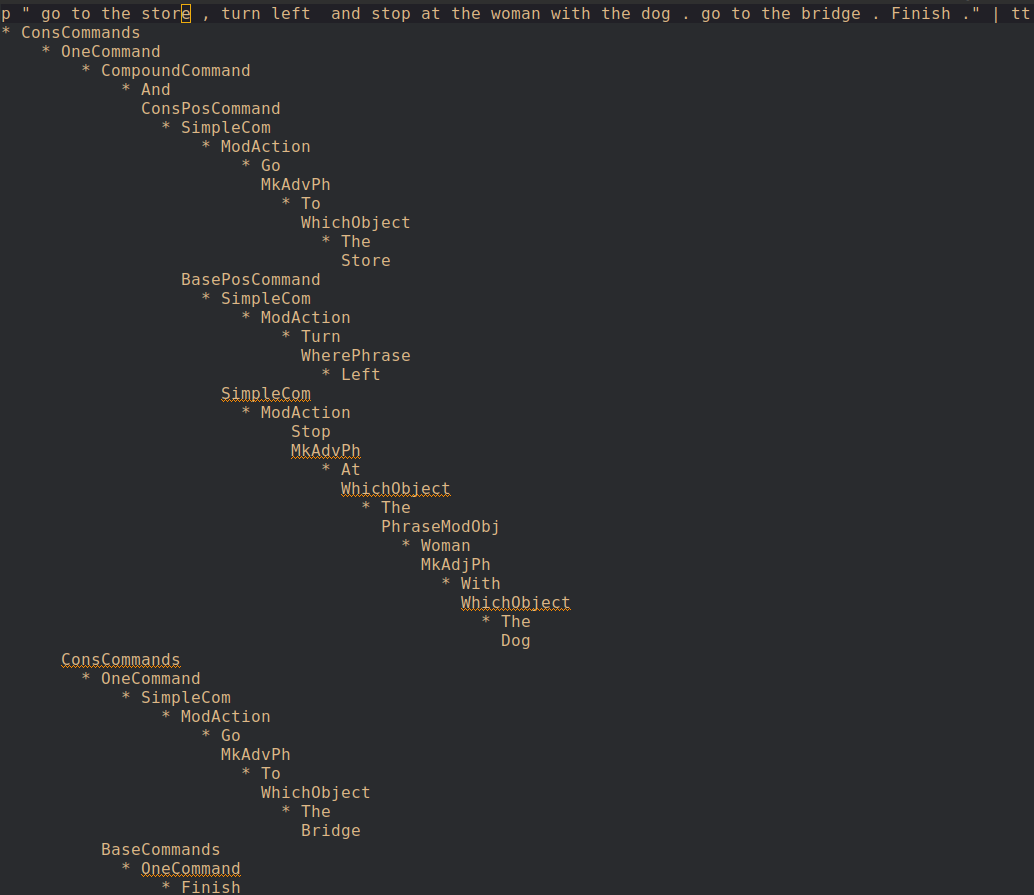
\includegraphics[width=90mm]{pics/wholeAST.png}
\end{figure}
\end{frame}

\begin{frame}
\fontsize{9pt}{10pt}\selectfont
\begin{exampleblock}{}
go to the store, turn left and stop at the woman with the dog. go to the bridge. finish.
\end{exampleblock}

\begin{figure}

\centering
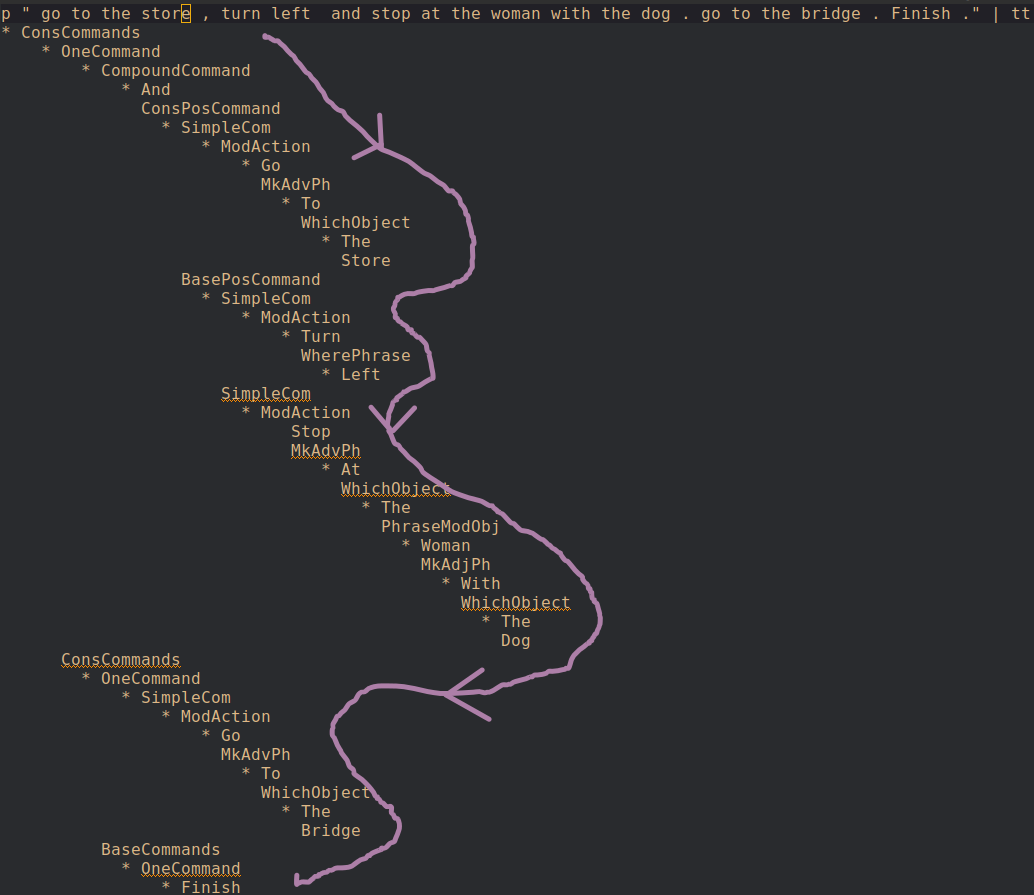
\includegraphics[width=90mm]{pics/WithArrow.png}
\end{figure}
\end{frame}

% the more "kinds" of branching there are, the more complicated
% can the different kinds of branching interact : this syntactic question
% manifests as a semantic one


\begin{frame}
\fontsize{9pt}{10pt}\selectfont
\begin{exampleblock}{}
go to the store, turn left and stop at the woman with the dog. go to the bridge.
finish.
\end{exampleblock}

\begin{figure}

\centering
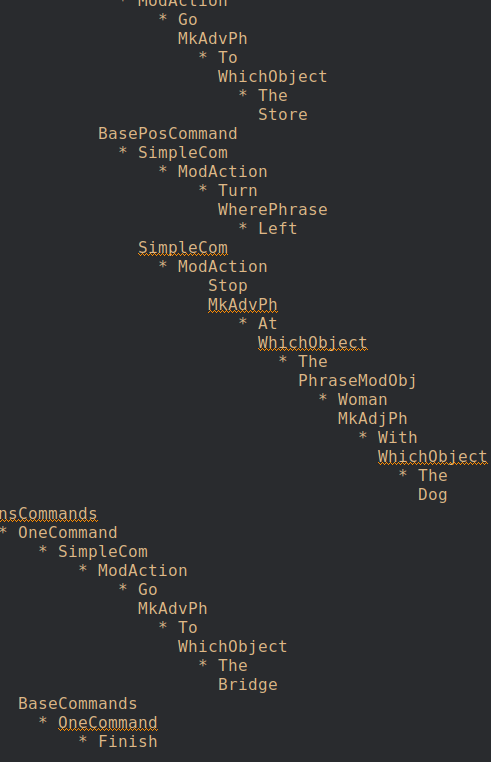
\includegraphics[width=50mm]{pics/zoomedScreenshot.png}
\end{figure}
\end{frame}

\begin{frame}
\fontsize{9pt}{10pt}\selectfont
\begin{exampleblock}{}
go to the store, turn left and stop at the woman with the dog. go to the bridge.
finish.
\end{exampleblock}

\begin{figure}

\centering
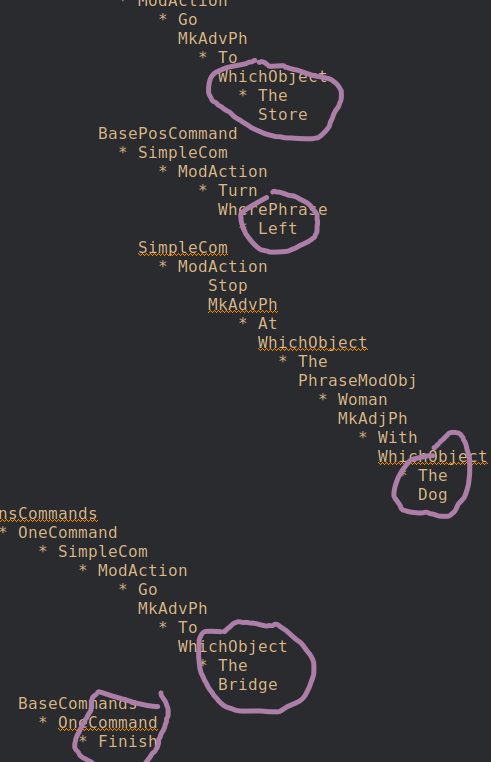
\includegraphics[width=50mm]{pics/circledZoom.png}
\end{figure}
\end{frame}


\begin{frame}[fragile]
\begin{exampleblock}{Alternative Interpretation}
go (to the store, turn left and stop (at the woman)) with the dog. 
\end{exampleblock}
\pause
\begin{verbatim}
ModAction
  * Stop
    MkAdvPh
      * At
        WhichObject
          * The
            Woman
MkAdvPh
  * With
    WhichObject
      * The
        Dog
\end{verbatim}
\pause
\begin{alertblock}{}
Need a temporal until operator, $U$, to construct a semantically justifiable interpretation
\end{alertblock}
\end{frame}

\section{Haskell}

\begin{frame}[fragile]
\frametitle{Haskell LTL}

\fontsize{9pt}{10pt}\selectfont
\begin{exampleblock}{}
go to the store, turn left and stop at the woman with the dog. go to the bridge.
finish.
\end{exampleblock}

\begin{verbatim}
  F (Meet
      (Atom "the_store")
      (F (Meet
          (Atom "turn_left")
          (F (Meet
               (Atom "the_woman_with_the_dog")
               (F (Meet
                    (Atom "the_bridge")
                    (G (Atom "FINISHED")))))))))
\end{verbatim}
\end{frame}

\begin{frame}[fragile]
\frametitle{Haskell Semantics}
\fontsize{9pt}{10pt}\selectfont
\begin{block}{}
Sequence of future states reveal a simple list flattening procedure which
amounts to an exceedingly simple denotational semantics
\end{block}
\pause
\begin{verbatim}
semantics :: GListCommands -> Phi
semantics x =
  let (GListCommands ((GOneCommand y) : _)) = normalizeList x
  in case y of
      q@(GSimpleCom a) -> astToAtom q
      (GCompoundCommand GAnd (GListPosCommand xs)) -> listCommand2LTL xs
\end{verbatim}
\pause
\begin{verbatim}
normalizeList ::  GListCommands -> GListCommands
  where
    normalizeNestedLists :: GListCommands -> GListPosCommand
      where
        normalizeListPosCommand :: GListPosCommand -> GListPosCommand
          where
            unSentence :: [GCommands] -> [GPosCommand]
            flattenSublist :: GPosCommand -> [GPosCommand]
            where
              getListPosCommands :: GListPosCommand -> [GPosCommand]
\end{verbatim}
\end{frame}





\begin{frame}
\frametitle{Temporal Logic}
\begin{itemize}[<+->]
\item Linear Temporal Logic (LTL)
\item Decidable model construction and decidable model checking
\item Many related temporal logics : CTL, MTL, STL, PrSTL, ...
\item Grounding of atomic propositions is central
\end{itemize}
\end{frame}

\begin{frame}
\begin{block}{Temporal Operators}
\begin{itemize}[<+->]
\item Unary temporal operators representing
\begin{itemize}[<+->]
\item the next state $X$
\item the existence of a future state $F$
\item the notion of henceforth, or forever $G$
\end{itemize}
\item Binary temporal operators representing the inclusive states in between two events $U$
\end{itemize}
\end{block}
\pause
\begin{exampleblock}{}
To ensure that every location $l_i$ eventually follows its predecessor
$l_{i-1}$, we target the following a class of formulas of the form $F\; (l_1 \wedge F\; (l_{2} \wedge ... F\; l_{n}))$
\end{exampleblock}

\end{frame}

\section{Agda}

\begin{frame}
\begin{code}[hide]%
\>[0]\AgdaKeyword{module}\AgdaSpace{}%
\AgdaModule{Syntax}\AgdaSpace{}%
\AgdaSymbol{(}\AgdaBound{Atom}\AgdaSpace{}%
\AgdaSymbol{:}\AgdaSpace{}%
\AgdaPrimitive{Set}\AgdaSymbol{)}\AgdaSpace{}%
\AgdaKeyword{where}\<%
\\
\>[0]\AgdaComment{-- Think Atom =FinSet}\<%
\end{code}
\begin{code}%
\>[0]\AgdaKeyword{data}\AgdaSpace{}%
\AgdaDatatype{ϕ}\AgdaSpace{}%
\AgdaSymbol{:}\AgdaSpace{}%
\AgdaPrimitive{Set}\AgdaSpace{}%
\AgdaKeyword{where}\<%
\\
\>[0][@{}l@{\AgdaIndent{0}}]%
\>[2]\AgdaInductiveConstructor{atom}%
\>[14]\AgdaSymbol{:}\AgdaSpace{}%
\AgdaBound{Atom}\AgdaSpace{}%
\AgdaSymbol{→}\AgdaSpace{}%
\AgdaDatatype{ϕ}\<%
\\
%
\>[2]\AgdaInductiveConstructor{⊥}\AgdaSpace{}%
\AgdaInductiveConstructor{⊤}%
\>[14]\AgdaSymbol{:}\AgdaSpace{}%
\AgdaDatatype{ϕ}\<%
\\
%
\>[2]\AgdaOperator{\AgdaInductiveConstructor{¬\AgdaUnderscore{}}}%
\>[14]\AgdaSymbol{:}\AgdaSpace{}%
\AgdaDatatype{ϕ}\AgdaSpace{}%
\AgdaSymbol{→}\AgdaSpace{}%
\AgdaDatatype{ϕ}\<%
\\
%
\>[2]\AgdaOperator{\AgdaInductiveConstructor{\AgdaUnderscore{}∨\AgdaUnderscore{}}}\AgdaSpace{}%
\AgdaOperator{\AgdaInductiveConstructor{\AgdaUnderscore{}∧\AgdaUnderscore{}}}\AgdaSpace{}%
\AgdaOperator{\AgdaInductiveConstructor{\AgdaUnderscore{}⇒\AgdaUnderscore{}}}\AgdaSpace{}%
\AgdaSymbol{:}\AgdaSpace{}%
\AgdaDatatype{ϕ}\AgdaSpace{}%
\AgdaSymbol{→}\AgdaSpace{}%
\AgdaDatatype{ϕ}\AgdaSpace{}%
\AgdaSymbol{→}\AgdaSpace{}%
\AgdaDatatype{ϕ}\<%
\\
%
\>[2]\AgdaInductiveConstructor{X}\AgdaSpace{}%
\AgdaInductiveConstructor{F}\AgdaSpace{}%
\AgdaInductiveConstructor{G}%
\>[14]\AgdaSymbol{:}\AgdaSpace{}%
\AgdaDatatype{ϕ}\AgdaSpace{}%
\AgdaSymbol{→}\AgdaSpace{}%
\AgdaDatatype{ϕ}\<%
\\
%
\>[2]\AgdaOperator{\AgdaInductiveConstructor{\AgdaUnderscore{}U\AgdaUnderscore{}}}\AgdaSpace{}%
\AgdaOperator{\AgdaInductiveConstructor{\AgdaUnderscore{}W\AgdaUnderscore{}}}\AgdaSpace{}%
\AgdaOperator{\AgdaInductiveConstructor{\AgdaUnderscore{}R\AgdaUnderscore{}}}\AgdaSpace{}%
\AgdaSymbol{:}\AgdaSpace{}%
\AgdaDatatype{ϕ}\AgdaSpace{}%
\AgdaSymbol{→}\AgdaSpace{}%
\AgdaDatatype{ϕ}\AgdaSpace{}%
\AgdaSymbol{→}\AgdaSpace{}%
\AgdaDatatype{ϕ}\<%
\end{code}
\begin{code}[hide]%
\>[0]\AgdaKeyword{open}\AgdaSpace{}%
\AgdaKeyword{import}\AgdaSpace{}%
\AgdaModule{Data.List}\<%
\\
%
\\[\AgdaEmptyExtraSkip]%
\>[0]\AgdaComment{-- that it automatically satisfies true, so if there are no location propositions}\<%
\\
\>[0]\AgdaComment{-- a trace is just a list of atoms}\<%
\\
\>[0]\AgdaComment{-- coverage versus surveillance patterns}\<%
\\
%
\\[\AgdaEmptyExtraSkip]%
\>[0]\AgdaComment{-- data atoms : Set where}\<%
\\
\>[0]\AgdaComment{--   corner : atoms}\<%
\\
\>[0]\AgdaComment{--   person : atoms}\<%
\\
\>[0]\AgdaComment{--   home   : atoms}\<%
\\
\>[0]\AgdaComment{--   cafe   : atoms}\<%
\\
%
\\[\AgdaEmptyExtraSkip]%
\>[0]\AgdaComment{--eventually visit all the ls}\<%
\\
\>[0]\AgdaFunction{visit}\AgdaSpace{}%
\AgdaSymbol{:}\AgdaSpace{}%
\AgdaDatatype{List}\AgdaSpace{}%
\AgdaBound{Atom}\AgdaSpace{}%
\AgdaSymbol{→}\AgdaSpace{}%
\AgdaDatatype{ϕ}\<%
\\
\>[0]\AgdaFunction{visit}\AgdaSpace{}%
\AgdaInductiveConstructor{[]}\AgdaSpace{}%
\AgdaSymbol{=}\AgdaSpace{}%
\AgdaInductiveConstructor{⊤}\<%
\\
\>[0]\AgdaFunction{visit}\AgdaSpace{}%
\AgdaSymbol{(}\AgdaBound{l}\AgdaSpace{}%
\AgdaOperator{\AgdaInductiveConstructor{∷}}\AgdaSpace{}%
\AgdaBound{ls}\AgdaSymbol{)}\AgdaSpace{}%
\AgdaSymbol{=}\AgdaSpace{}%
\AgdaSymbol{(}\AgdaInductiveConstructor{F}\AgdaSpace{}%
\AgdaSymbol{(}\AgdaInductiveConstructor{atom}\AgdaSpace{}%
\AgdaBound{l}\AgdaSymbol{))}\AgdaSpace{}%
\AgdaOperator{\AgdaInductiveConstructor{∧}}\AgdaSpace{}%
\AgdaFunction{visit}\AgdaSpace{}%
\AgdaBound{ls}\<%
\\
%
\\[\AgdaEmptyExtraSkip]%
\>[0]\AgdaComment{-- eventually replace eventually with efficiently : (i.e. minimize energy such that you get there)}\<%
\\
%
\\[\AgdaEmptyExtraSkip]%
\>[0]\AgdaComment{--eventually visit l1, and then eventually visit l2,}\<%
\\
\>[0]\AgdaFunction{sequentialVisit}\AgdaSpace{}%
\AgdaSymbol{:}\AgdaSpace{}%
\AgdaDatatype{List}\AgdaSpace{}%
\AgdaBound{Atom}\AgdaSpace{}%
\AgdaSymbol{→}\AgdaSpace{}%
\AgdaDatatype{ϕ}\<%
\\
\>[0]\AgdaFunction{sequentialVisit}\AgdaSpace{}%
\AgdaInductiveConstructor{[]}\AgdaSpace{}%
\AgdaSymbol{=}\AgdaSpace{}%
\AgdaInductiveConstructor{⊤}\<%
\\
\>[0]\AgdaFunction{sequentialVisit}\AgdaSpace{}%
\AgdaSymbol{(}\AgdaBound{l}\AgdaSpace{}%
\AgdaOperator{\AgdaInductiveConstructor{∷}}\AgdaSpace{}%
\AgdaBound{ls}\AgdaSymbol{)}\AgdaSpace{}%
\AgdaSymbol{=}\AgdaSpace{}%
\AgdaInductiveConstructor{F}\AgdaSpace{}%
\AgdaSymbol{(}\AgdaInductiveConstructor{atom}\AgdaSpace{}%
\AgdaBound{l}\AgdaSpace{}%
\AgdaOperator{\AgdaInductiveConstructor{∧}}\AgdaSpace{}%
\AgdaFunction{sequentialVisit}\AgdaSpace{}%
\AgdaBound{ls}\AgdaSymbol{)}\<%
\\
%
\\[\AgdaEmptyExtraSkip]%
\>[0]\AgdaComment{-- suppose the driver doesn't actually care if they visit all the locations, as}\<%
\\
\>[0]\AgdaComment{-- long as they get to the last location}\<%
\\
\>[0]\AgdaFunction{weakSequentialVisit}\AgdaSpace{}%
\AgdaSymbol{:}\AgdaSpace{}%
\AgdaDatatype{List}\AgdaSpace{}%
\AgdaBound{Atom}\AgdaSpace{}%
\AgdaSymbol{→}\AgdaSpace{}%
\AgdaDatatype{ϕ}\<%
\\
\>[0]\AgdaFunction{weakSequentialVisit}\AgdaSpace{}%
\AgdaInductiveConstructor{[]}\AgdaSpace{}%
\AgdaSymbol{=}\AgdaSpace{}%
\AgdaInductiveConstructor{⊤}\<%
\\
\>[0]\AgdaFunction{weakSequentialVisit}\AgdaSpace{}%
\AgdaBound{lss}\AgdaSymbol{@(}\AgdaBound{l}\AgdaSpace{}%
\AgdaOperator{\AgdaInductiveConstructor{∷}}\AgdaSpace{}%
\AgdaBound{ls}\AgdaSymbol{)}\AgdaSpace{}%
\AgdaSymbol{=}\AgdaSpace{}%
\AgdaFunction{sequentialVisit}\AgdaSpace{}%
\AgdaBound{lss}\AgdaSpace{}%
\AgdaOperator{\AgdaInductiveConstructor{∨}}\AgdaSpace{}%
\AgdaFunction{weakSequentialVisit}\AgdaSpace{}%
\AgdaBound{ls}\<%
\\
%
\\[\AgdaEmptyExtraSkip]%
\>[0]\AgdaComment{-- ordering condition}\<%
\\
\>[0]\AgdaComment{-- don't visit li+1 until you've visited li}\<%
\\
\>[0]\AgdaFunction{predecessorPrecedesSuccessor}\AgdaSpace{}%
\AgdaSymbol{:}\AgdaSpace{}%
\AgdaDatatype{List}\AgdaSpace{}%
\AgdaBound{Atom}\AgdaSpace{}%
\AgdaSymbol{→}\AgdaSpace{}%
\AgdaDatatype{ϕ}\<%
\\
\>[0]\AgdaFunction{predecessorPrecedesSuccessor}\AgdaSpace{}%
\AgdaInductiveConstructor{[]}\AgdaSpace{}%
\AgdaSymbol{=}\AgdaSpace{}%
\AgdaInductiveConstructor{⊤}\<%
\\
\>[0]\AgdaFunction{predecessorPrecedesSuccessor}\AgdaSpace{}%
\AgdaSymbol{(}\AgdaBound{l}\AgdaSpace{}%
\AgdaOperator{\AgdaInductiveConstructor{∷}}\AgdaSpace{}%
\AgdaInductiveConstructor{[]}\AgdaSymbol{)}\AgdaSpace{}%
\AgdaSymbol{=}\AgdaSpace{}%
\AgdaInductiveConstructor{⊤}\<%
\\
\>[0]\AgdaFunction{predecessorPrecedesSuccessor}\AgdaSpace{}%
\AgdaSymbol{(}\AgdaBound{lᵢ}\AgdaSpace{}%
\AgdaOperator{\AgdaInductiveConstructor{∷}}\AgdaSpace{}%
\AgdaBound{lᵢ₊₁}\AgdaSpace{}%
\AgdaOperator{\AgdaInductiveConstructor{∷}}\AgdaSpace{}%
\AgdaBound{ls}\AgdaSymbol{)}\AgdaSpace{}%
\AgdaSymbol{=}\<%
\\
\>[0][@{}l@{\AgdaIndent{0}}]%
\>[2]\AgdaSymbol{((}\AgdaOperator{\AgdaInductiveConstructor{¬}}\AgdaSpace{}%
\AgdaInductiveConstructor{atom}\AgdaSpace{}%
\AgdaBound{lᵢ₊₁}\AgdaSymbol{)}\AgdaSpace{}%
\AgdaOperator{\AgdaInductiveConstructor{U}}\AgdaSpace{}%
\AgdaInductiveConstructor{atom}\AgdaSpace{}%
\AgdaBound{lᵢ}\AgdaSymbol{)}\AgdaSpace{}%
\AgdaOperator{\AgdaInductiveConstructor{∧}}\AgdaSpace{}%
\AgdaFunction{predecessorPrecedesSuccessor}\AgdaSpace{}%
\AgdaSymbol{(}\AgdaBound{lᵢ₊₁}\AgdaSpace{}%
\AgdaOperator{\AgdaInductiveConstructor{∷}}\AgdaSpace{}%
\AgdaBound{ls}\AgdaSymbol{)}\<%
\\
%
\\[\AgdaEmptyExtraSkip]%
\>[0]\AgdaFunction{orderedVisit}\AgdaSpace{}%
\AgdaSymbol{:}\AgdaSpace{}%
\AgdaDatatype{List}\AgdaSpace{}%
\AgdaBound{Atom}\AgdaSpace{}%
\AgdaSymbol{→}\AgdaSpace{}%
\AgdaDatatype{ϕ}\<%
\\
\>[0]\AgdaFunction{orderedVisit}\AgdaSpace{}%
\AgdaBound{ls}\AgdaSpace{}%
\AgdaSymbol{=}\AgdaSpace{}%
\AgdaFunction{sequentialVisit}\AgdaSpace{}%
\AgdaBound{ls}\AgdaSpace{}%
\AgdaOperator{\AgdaInductiveConstructor{∧}}\AgdaSpace{}%
\AgdaFunction{predecessorPrecedesSuccessor}\AgdaSpace{}%
\AgdaBound{ls}\<%
\\
%
\\[\AgdaEmptyExtraSkip]%
\>[0]\AgdaComment{-- strictness condition}\<%
\\
\>[0]\AgdaComment{-- don't visit a location twice}\<%
\\
\>[0]\AgdaComment{-- probably not realistic for our example}\<%
\\
\>[0]\AgdaComment{-- everything should also depend on the location of the vehicle}\<%
\\
\>[0]\AgdaComment{-- past temporal operators should be used to judge the success of a mission}\<%
\\
\>[0]\AgdaFunction{strictSeq}\AgdaSpace{}%
\AgdaSymbol{:}\AgdaSpace{}%
\AgdaDatatype{List}\AgdaSpace{}%
\AgdaBound{Atom}\AgdaSpace{}%
\AgdaSymbol{→}\AgdaSpace{}%
\AgdaDatatype{ϕ}\<%
\\
\>[0]\AgdaFunction{strictSeq}\AgdaSpace{}%
\AgdaInductiveConstructor{[]}\AgdaSpace{}%
\AgdaSymbol{=}\AgdaSpace{}%
\AgdaInductiveConstructor{⊤}\<%
\\
\>[0]\AgdaFunction{strictSeq}\AgdaSpace{}%
\AgdaSymbol{(}\AgdaBound{l}\AgdaSpace{}%
\AgdaOperator{\AgdaInductiveConstructor{∷}}\AgdaSpace{}%
\AgdaInductiveConstructor{[]}\AgdaSymbol{)}\AgdaSpace{}%
\AgdaSymbol{=}\AgdaSpace{}%
\AgdaInductiveConstructor{⊤}\<%
\\
\>[0]\AgdaFunction{strictSeq}\AgdaSpace{}%
\AgdaSymbol{(}\AgdaBound{lᵢ}\AgdaSpace{}%
\AgdaOperator{\AgdaInductiveConstructor{∷}}\AgdaSpace{}%
\AgdaBound{lᵢ₊₁}\AgdaSpace{}%
\AgdaOperator{\AgdaInductiveConstructor{∷}}\AgdaSpace{}%
\AgdaBound{ls}\AgdaSymbol{)}\AgdaSpace{}%
\AgdaSymbol{=}\AgdaSpace{}%
\AgdaSymbol{((}\AgdaOperator{\AgdaInductiveConstructor{¬}}\AgdaSpace{}%
\AgdaInductiveConstructor{atom}\AgdaSpace{}%
\AgdaBound{lᵢ₊₁}\AgdaSymbol{)}\AgdaSpace{}%
\AgdaOperator{\AgdaInductiveConstructor{U}}\AgdaSpace{}%
\AgdaSymbol{(}\AgdaInductiveConstructor{atom}\AgdaSpace{}%
\AgdaBound{lᵢ}\AgdaSpace{}%
\AgdaOperator{\AgdaInductiveConstructor{∧}}\AgdaSpace{}%
\AgdaInductiveConstructor{X}\AgdaSpace{}%
\AgdaSymbol{((}\AgdaOperator{\AgdaInductiveConstructor{¬}}\AgdaSpace{}%
\AgdaInductiveConstructor{atom}\AgdaSpace{}%
\AgdaBound{lᵢ}\AgdaSymbol{)}\AgdaSpace{}%
\AgdaOperator{\AgdaInductiveConstructor{U}}\AgdaSpace{}%
\AgdaInductiveConstructor{atom}\AgdaSpace{}%
\AgdaBound{lᵢ₊₁}\AgdaSymbol{)))}\AgdaSpace{}%
\AgdaOperator{\AgdaInductiveConstructor{∧}}\AgdaSpace{}%
\AgdaFunction{strictSeq}\AgdaSpace{}%
\AgdaSymbol{(}\AgdaBound{lᵢ₊₁}\AgdaSpace{}%
\AgdaOperator{\AgdaInductiveConstructor{∷}}\AgdaSpace{}%
\AgdaBound{ls}\AgdaSymbol{)}\<%
\\
%
\\[\AgdaEmptyExtraSkip]%
\>[0]\AgdaFunction{strictOrderedVisit}\AgdaSpace{}%
\AgdaSymbol{:}\AgdaSpace{}%
\AgdaDatatype{List}\AgdaSpace{}%
\AgdaBound{Atom}\AgdaSpace{}%
\AgdaSymbol{→}\AgdaSpace{}%
\AgdaDatatype{ϕ}\<%
\\
\>[0]\AgdaFunction{strictOrderedVisit}\AgdaSpace{}%
\AgdaBound{ls}\AgdaSpace{}%
\AgdaSymbol{=}\AgdaSpace{}%
\AgdaFunction{orderedVisit}\AgdaSpace{}%
\AgdaBound{ls}\AgdaSpace{}%
\AgdaOperator{\AgdaInductiveConstructor{∧}}\AgdaSpace{}%
\AgdaFunction{strictSeq}\AgdaSpace{}%
\AgdaBound{ls}\<%
\\
%
\\[\AgdaEmptyExtraSkip]%
\>[0]\AgdaComment{-- define a satisfaction for a trace -- only care about the finite case, but really we should generalize this}\<%
\\
\>[0]\AgdaComment{-- can ask if a trace satisisfies a formula}\<%
\\
%
\\[\AgdaEmptyExtraSkip]%
\>[0]\AgdaComment{--Mission specifications}\<%
\\
\>[0]\AgdaComment{-- are used, among others, to synthesize, verify, simulate or guide}\<%
\\
\>[0]\AgdaComment{-- the engineering of robot software}\<%
\\
%
\\[\AgdaEmptyExtraSkip]%
\>[0]\AgdaComment{--fair visit and patrolling, could be interpreted with respect to taking the cab around}\<%
\\
\>[0]\AgdaComment{-- a trace is just a path where the labeller is restricted to singleton sets}\<%
\\
%
\\[\AgdaEmptyExtraSkip]%
\>[0]\AgdaComment{-- G (isRed -> (break U vel == 0) U isGreen) (unless there is an ambulance)}\<%
\\
%
\\[\AgdaEmptyExtraSkip]%
\>[0]\AgdaComment{-- stop is really a slow and stay stop}\<%
\\
%
\\[\AgdaEmptyExtraSkip]%
\>[0]\AgdaComment{-- G (isGreen -> Go)}\<%
\\
%
\\[\AgdaEmptyExtraSkip]%
\>[0]\AgdaComment{-- globally, obey}\<%
\end{code}

\end{frame}

\begin{frame}
\begin{exampleblock}{}
$F\; (l_1 \wedge F\; (l_{2} \wedge ... F\; l_{n}))$
\end{exampleblock}
\begin{code}[hide]%
\>[0]\AgdaKeyword{module}\AgdaSpace{}%
\AgdaModule{Syntaxx}\AgdaSpace{}%
\AgdaSymbol{(}\AgdaBound{Atom}\AgdaSpace{}%
\AgdaSymbol{:}\AgdaSpace{}%
\AgdaPrimitive{Set}\AgdaSymbol{)}\AgdaSpace{}%
\AgdaKeyword{where}\<%
\\
\>[0]\AgdaComment{-- Think Atom =FinSet}\<%
\end{code}
\begin{code}[hide]%
\>[0]\AgdaKeyword{data}\AgdaSpace{}%
\AgdaDatatype{ϕ}\AgdaSpace{}%
\AgdaSymbol{:}\AgdaSpace{}%
\AgdaPrimitive{Set}\AgdaSpace{}%
\AgdaKeyword{where}\<%
\\
\>[0][@{}l@{\AgdaIndent{0}}]%
\>[2]\AgdaInductiveConstructor{atom}%
\>[14]\AgdaSymbol{:}\AgdaSpace{}%
\AgdaBound{Atom}\AgdaSpace{}%
\AgdaSymbol{→}\AgdaSpace{}%
\AgdaDatatype{ϕ}\<%
\\
%
\>[2]\AgdaInductiveConstructor{⊥}\AgdaSpace{}%
\AgdaInductiveConstructor{⊤}%
\>[14]\AgdaSymbol{:}\AgdaSpace{}%
\AgdaDatatype{ϕ}\<%
\\
%
\>[2]\AgdaOperator{\AgdaInductiveConstructor{¬\AgdaUnderscore{}}}%
\>[14]\AgdaSymbol{:}\AgdaSpace{}%
\AgdaDatatype{ϕ}\AgdaSpace{}%
\AgdaSymbol{→}\AgdaSpace{}%
\AgdaDatatype{ϕ}\<%
\\
%
\>[2]\AgdaOperator{\AgdaInductiveConstructor{\AgdaUnderscore{}∨\AgdaUnderscore{}}}\AgdaSpace{}%
\AgdaOperator{\AgdaInductiveConstructor{\AgdaUnderscore{}∧\AgdaUnderscore{}}}\AgdaSpace{}%
\AgdaOperator{\AgdaInductiveConstructor{\AgdaUnderscore{}⇒\AgdaUnderscore{}}}\AgdaSpace{}%
\AgdaSymbol{:}\AgdaSpace{}%
\AgdaDatatype{ϕ}\AgdaSpace{}%
\AgdaSymbol{→}\AgdaSpace{}%
\AgdaDatatype{ϕ}\AgdaSpace{}%
\AgdaSymbol{→}\AgdaSpace{}%
\AgdaDatatype{ϕ}\<%
\\
%
\>[2]\AgdaInductiveConstructor{X}\AgdaSpace{}%
\AgdaInductiveConstructor{F}\AgdaSpace{}%
\AgdaInductiveConstructor{G}%
\>[14]\AgdaSymbol{:}\AgdaSpace{}%
\AgdaDatatype{ϕ}\AgdaSpace{}%
\AgdaSymbol{→}\AgdaSpace{}%
\AgdaDatatype{ϕ}\<%
\\
%
\>[2]\AgdaOperator{\AgdaInductiveConstructor{\AgdaUnderscore{}U\AgdaUnderscore{}}}\AgdaSpace{}%
\AgdaOperator{\AgdaInductiveConstructor{\AgdaUnderscore{}W\AgdaUnderscore{}}}\AgdaSpace{}%
\AgdaOperator{\AgdaInductiveConstructor{\AgdaUnderscore{}R\AgdaUnderscore{}}}\AgdaSpace{}%
\AgdaSymbol{:}\AgdaSpace{}%
\AgdaDatatype{ϕ}\AgdaSpace{}%
\AgdaSymbol{→}\AgdaSpace{}%
\AgdaDatatype{ϕ}\AgdaSpace{}%
\AgdaSymbol{→}\AgdaSpace{}%
\AgdaDatatype{ϕ}\<%
\end{code}
\begin{code}[hide]%
\>[0]\AgdaKeyword{open}\AgdaSpace{}%
\AgdaKeyword{import}\AgdaSpace{}%
\AgdaModule{Data.List}\<%
\\
%
\\[\AgdaEmptyExtraSkip]%
\>[0]\AgdaComment{-- that it automatically satisfies true, so if there are no location propositions}\<%
\\
\>[0]\AgdaComment{-- a trace is just a list of atoms}\<%
\\
\>[0]\AgdaComment{-- coverage versus surveillance patterns}\<%
\\
%
\\[\AgdaEmptyExtraSkip]%
\>[0]\AgdaComment{-- data atoms : Set where}\<%
\\
\>[0]\AgdaComment{--   corner : atoms}\<%
\\
\>[0]\AgdaComment{--   person : atoms}\<%
\\
\>[0]\AgdaComment{--   home   : atoms}\<%
\\
\>[0]\AgdaComment{--   cafe   : atoms}\<%
\\
\>[0]\<%
\end{code}
\begin{code}%
\>[0]\AgdaFunction{visit}\AgdaSpace{}%
\AgdaSymbol{:}\AgdaSpace{}%
\AgdaDatatype{List}\AgdaSpace{}%
\AgdaBound{Atom}\AgdaSpace{}%
\AgdaSymbol{→}\AgdaSpace{}%
\AgdaDatatype{ϕ}\<%
\\
\>[0]\AgdaFunction{visit}\AgdaSpace{}%
\AgdaInductiveConstructor{[]}\AgdaSpace{}%
\AgdaSymbol{=}\AgdaSpace{}%
\AgdaInductiveConstructor{⊤}\<%
\\
\>[0]\AgdaFunction{visit}\AgdaSpace{}%
\AgdaSymbol{(}\AgdaBound{l}\AgdaSpace{}%
\AgdaOperator{\AgdaInductiveConstructor{∷}}\AgdaSpace{}%
\AgdaBound{ls}\AgdaSymbol{)}\AgdaSpace{}%
\AgdaSymbol{=}\AgdaSpace{}%
\AgdaSymbol{(}\AgdaInductiveConstructor{F}\AgdaSpace{}%
\AgdaSymbol{(}\AgdaInductiveConstructor{atom}\AgdaSpace{}%
\AgdaBound{l}\AgdaSymbol{))}\AgdaSpace{}%
\AgdaOperator{\AgdaInductiveConstructor{∧}}\AgdaSpace{}%
\AgdaFunction{visit}\AgdaSpace{}%
\AgdaBound{ls}\<%
\\
%
\\[\AgdaEmptyExtraSkip]%
\>[0]\AgdaFunction{sequentialVisit}\AgdaSpace{}%
\AgdaSymbol{:}\AgdaSpace{}%
\AgdaDatatype{List}\AgdaSpace{}%
\AgdaBound{Atom}\AgdaSpace{}%
\AgdaSymbol{→}\AgdaSpace{}%
\AgdaDatatype{ϕ}\<%
\\
\>[0]\AgdaFunction{sequentialVisit}\AgdaSpace{}%
\AgdaInductiveConstructor{[]}\AgdaSpace{}%
\AgdaSymbol{=}\AgdaSpace{}%
\AgdaInductiveConstructor{⊤}\<%
\\
\>[0]\AgdaFunction{sequentialVisit}\AgdaSpace{}%
\AgdaSymbol{(}\AgdaBound{l}\AgdaSpace{}%
\AgdaOperator{\AgdaInductiveConstructor{∷}}\AgdaSpace{}%
\AgdaBound{ls}\AgdaSymbol{)}\AgdaSpace{}%
\AgdaSymbol{=}\AgdaSpace{}%
\AgdaInductiveConstructor{F}\AgdaSpace{}%
\AgdaSymbol{(}\AgdaInductiveConstructor{atom}\AgdaSpace{}%
\AgdaBound{l}\AgdaSpace{}%
\AgdaOperator{\AgdaInductiveConstructor{∧}}\AgdaSpace{}%
\AgdaFunction{sequentialVisit}\AgdaSpace{}%
\AgdaBound{ls}\AgdaSymbol{)}\<%
\\
%
\\[\AgdaEmptyExtraSkip]%
\>[0]\AgdaFunction{predecessorPrecedesSuccessor}\AgdaSpace{}%
\AgdaSymbol{:}\AgdaSpace{}%
\AgdaDatatype{List}\AgdaSpace{}%
\AgdaBound{Atom}\AgdaSpace{}%
\AgdaSymbol{→}\AgdaSpace{}%
\AgdaDatatype{ϕ}\<%
\\
\>[0]\AgdaFunction{predecessorPrecedesSuccessor}\AgdaSpace{}%
\AgdaInductiveConstructor{[]}\AgdaSpace{}%
\AgdaSymbol{=}\AgdaSpace{}%
\AgdaInductiveConstructor{⊤}\<%
\\
\>[0]\AgdaFunction{predecessorPrecedesSuccessor}\AgdaSpace{}%
\AgdaSymbol{(}\AgdaBound{l}\AgdaSpace{}%
\AgdaOperator{\AgdaInductiveConstructor{∷}}\AgdaSpace{}%
\AgdaInductiveConstructor{[]}\AgdaSymbol{)}\AgdaSpace{}%
\AgdaSymbol{=}\AgdaSpace{}%
\AgdaInductiveConstructor{⊤}\<%
\\
\>[0]\AgdaFunction{predecessorPrecedesSuccessor}\AgdaSpace{}%
\AgdaSymbol{(}\AgdaBound{l}\AgdaSpace{}%
\AgdaOperator{\AgdaInductiveConstructor{∷}}\AgdaSpace{}%
\AgdaBound{l'}\AgdaSpace{}%
\AgdaOperator{\AgdaInductiveConstructor{∷}}\AgdaSpace{}%
\AgdaBound{ls}\AgdaSymbol{)}\AgdaSpace{}%
\AgdaSymbol{=}\<%
\\
\>[0][@{}l@{\AgdaIndent{0}}]%
\>[2]\AgdaSymbol{((}\AgdaOperator{\AgdaInductiveConstructor{¬}}\AgdaSpace{}%
\AgdaInductiveConstructor{atom}\AgdaSpace{}%
\AgdaBound{l'}\AgdaSymbol{)}\AgdaSpace{}%
\AgdaOperator{\AgdaInductiveConstructor{U}}\AgdaSpace{}%
\AgdaInductiveConstructor{atom}\AgdaSpace{}%
\AgdaBound{l}\AgdaSymbol{)}\AgdaSpace{}%
\AgdaOperator{\AgdaInductiveConstructor{∧}}\AgdaSpace{}%
\AgdaFunction{predecessorPrecedesSuccessor}\AgdaSpace{}%
\AgdaSymbol{(}\AgdaBound{l'}\AgdaSpace{}%
\AgdaOperator{\AgdaInductiveConstructor{∷}}\AgdaSpace{}%
\AgdaBound{ls}\AgdaSymbol{)}\<%
\\
%
\\[\AgdaEmptyExtraSkip]%
\>[0]\AgdaFunction{orderedVisit}\AgdaSpace{}%
\AgdaSymbol{:}\AgdaSpace{}%
\AgdaDatatype{List}\AgdaSpace{}%
\AgdaBound{Atom}\AgdaSpace{}%
\AgdaSymbol{→}\AgdaSpace{}%
\AgdaDatatype{ϕ}\<%
\\
\>[0]\AgdaFunction{orderedVisit}\AgdaSpace{}%
\AgdaBound{ls}\AgdaSpace{}%
\AgdaSymbol{=}\AgdaSpace{}%
\AgdaFunction{sequentialVisit}\AgdaSpace{}%
\AgdaBound{ls}\AgdaSpace{}%
\AgdaOperator{\AgdaInductiveConstructor{∧}}\AgdaSpace{}%
\AgdaFunction{predecessorPrecedesSuccessor}\AgdaSpace{}%
\AgdaBound{ls}\<%
\end{code}
\begin{code}[hide]%
\>[0]\<%
\\
\>[0]\AgdaComment{-- strictness condition}\<%
\\
\>[0]\AgdaComment{-- don't visit a location twice}\<%
\\
\>[0]\AgdaComment{-- probably not realistic for our example}\<%
\\
\>[0]\AgdaComment{-- everything should also depend on the location of the vehicle}\<%
\\
\>[0]\AgdaComment{-- past temporal operators should be used to judge the success of a mission}\<%
\\
\>[0]\AgdaFunction{strictSeq}\AgdaSpace{}%
\AgdaSymbol{:}\AgdaSpace{}%
\AgdaDatatype{List}\AgdaSpace{}%
\AgdaBound{Atom}\AgdaSpace{}%
\AgdaSymbol{→}\AgdaSpace{}%
\AgdaDatatype{ϕ}\<%
\\
\>[0]\AgdaFunction{strictSeq}\AgdaSpace{}%
\AgdaInductiveConstructor{[]}\AgdaSpace{}%
\AgdaSymbol{=}\AgdaSpace{}%
\AgdaInductiveConstructor{⊤}\<%
\\
\>[0]\AgdaFunction{strictSeq}\AgdaSpace{}%
\AgdaSymbol{(}\AgdaBound{l}\AgdaSpace{}%
\AgdaOperator{\AgdaInductiveConstructor{∷}}\AgdaSpace{}%
\AgdaInductiveConstructor{[]}\AgdaSymbol{)}\AgdaSpace{}%
\AgdaSymbol{=}\AgdaSpace{}%
\AgdaInductiveConstructor{⊤}\<%
\\
\>[0]\AgdaFunction{strictSeq}\AgdaSpace{}%
\AgdaSymbol{(}\AgdaBound{lᵢ}\AgdaSpace{}%
\AgdaOperator{\AgdaInductiveConstructor{∷}}\AgdaSpace{}%
\AgdaBound{lᵢ₊₁}\AgdaSpace{}%
\AgdaOperator{\AgdaInductiveConstructor{∷}}\AgdaSpace{}%
\AgdaBound{ls}\AgdaSymbol{)}\AgdaSpace{}%
\AgdaSymbol{=}\AgdaSpace{}%
\AgdaSymbol{((}\AgdaOperator{\AgdaInductiveConstructor{¬}}\AgdaSpace{}%
\AgdaInductiveConstructor{atom}\AgdaSpace{}%
\AgdaBound{lᵢ₊₁}\AgdaSymbol{)}\AgdaSpace{}%
\AgdaOperator{\AgdaInductiveConstructor{U}}\AgdaSpace{}%
\AgdaSymbol{(}\AgdaInductiveConstructor{atom}\AgdaSpace{}%
\AgdaBound{lᵢ}\AgdaSpace{}%
\AgdaOperator{\AgdaInductiveConstructor{∧}}\AgdaSpace{}%
\AgdaInductiveConstructor{X}\AgdaSpace{}%
\AgdaSymbol{((}\AgdaOperator{\AgdaInductiveConstructor{¬}}\AgdaSpace{}%
\AgdaInductiveConstructor{atom}\AgdaSpace{}%
\AgdaBound{lᵢ}\AgdaSymbol{)}\AgdaSpace{}%
\AgdaOperator{\AgdaInductiveConstructor{U}}\AgdaSpace{}%
\AgdaInductiveConstructor{atom}\AgdaSpace{}%
\AgdaBound{lᵢ₊₁}\AgdaSymbol{)))}\AgdaSpace{}%
\AgdaOperator{\AgdaInductiveConstructor{∧}}\AgdaSpace{}%
\AgdaFunction{strictSeq}\AgdaSpace{}%
\AgdaSymbol{(}\AgdaBound{lᵢ₊₁}\AgdaSpace{}%
\AgdaOperator{\AgdaInductiveConstructor{∷}}\AgdaSpace{}%
\AgdaBound{ls}\AgdaSymbol{)}\<%
\\
%
\\[\AgdaEmptyExtraSkip]%
\>[0]\AgdaFunction{strictOrderedVisit}\AgdaSpace{}%
\AgdaSymbol{:}\AgdaSpace{}%
\AgdaDatatype{List}\AgdaSpace{}%
\AgdaBound{Atom}\AgdaSpace{}%
\AgdaSymbol{→}\AgdaSpace{}%
\AgdaDatatype{ϕ}\<%
\\
\>[0]\AgdaFunction{strictOrderedVisit}\AgdaSpace{}%
\AgdaBound{ls}\AgdaSpace{}%
\AgdaSymbol{=}\AgdaSpace{}%
\AgdaFunction{orderedVisit}\AgdaSpace{}%
\AgdaBound{ls}\AgdaSpace{}%
\AgdaOperator{\AgdaInductiveConstructor{∧}}\AgdaSpace{}%
\AgdaFunction{strictSeq}\AgdaSpace{}%
\AgdaBound{ls}\<%
\\
%
\\[\AgdaEmptyExtraSkip]%
\>[0]\AgdaComment{-- define a satisfaction for a trace -- only care about the finite case, but really we should generalize this}\<%
\\
\>[0]\AgdaComment{-- can ask if a trace satisisfies a formula}\<%
\\
%
\\[\AgdaEmptyExtraSkip]%
\>[0]\AgdaComment{--Mission specifications}\<%
\\
\>[0]\AgdaComment{-- are used, among others, to synthesize, verify, simulate or guide}\<%
\\
\>[0]\AgdaComment{-- the engineering of robot software}\<%
\\
%
\\[\AgdaEmptyExtraSkip]%
\>[0]\AgdaComment{--fair visit and patrolling, could be interpreted with respect to taking the cab around}\<%
\\
\>[0]\AgdaComment{-- a trace is just a path where the labeller is restricted to singleton sets}\<%
\\
%
\\[\AgdaEmptyExtraSkip]%
\>[0]\AgdaComment{-- G (isRed -> (break U vel == 0) U isGreen) (unless there is an ambulance)}\<%
\\
%
\\[\AgdaEmptyExtraSkip]%
\>[0]\AgdaComment{-- stop is really a slow and stay stop}\<%
\\
%
\\[\AgdaEmptyExtraSkip]%
\>[0]\AgdaComment{-- G (isGreen -> Go)}\<%
\\
%
\\[\AgdaEmptyExtraSkip]%
\>[0]\AgdaComment{-- globally, obey}\<%
\end{code}

\end{frame}

\begin{frame}
\begin{code}[hide]%
\>[0]\AgdaKeyword{module}\AgdaSpace{}%
\AgdaModule{Model}\AgdaSpace{}%
\AgdaKeyword{where}\<%
\\
%
\\[\AgdaEmptyExtraSkip]%
\>[0]\AgdaKeyword{open}\AgdaSpace{}%
\AgdaKeyword{import}\AgdaSpace{}%
\AgdaModule{Support}\<%
\\
%
\\[\AgdaEmptyExtraSkip]%
\>[0]\AgdaComment{\{-
Refactored so-as to allow for easier (more infomrative) proofs
Originally had
L : State → 𝑃 Atom
-\}}\<%
\end{code}
\begin{code}%
\>[0]\AgdaKeyword{record}\AgdaSpace{}%
\AgdaRecord{𝑀}\AgdaSpace{}%
\AgdaSymbol{(}\AgdaBound{Atom}\AgdaSpace{}%
\AgdaSymbol{:}\AgdaSpace{}%
\AgdaPrimitive{Set}\AgdaSymbol{)}\AgdaSpace{}%
\AgdaSymbol{:}\AgdaSpace{}%
\AgdaPrimitive{Set1}\AgdaSpace{}%
\AgdaKeyword{where}\<%
\\
\>[0][@{}l@{\AgdaIndent{0}}]%
\>[2]\AgdaKeyword{field}\<%
\\
\>[2][@{}l@{\AgdaIndent{0}}]%
\>[4]\AgdaField{State}\AgdaSpace{}%
\AgdaSymbol{:}\AgdaSpace{}%
\AgdaPrimitive{Set}\<%
\\
%
\>[4]\AgdaOperator{\AgdaField{\AgdaUnderscore{}⟶\AgdaUnderscore{}}}\AgdaSpace{}%
\AgdaSymbol{:}\AgdaSpace{}%
\AgdaFunction{rel}\AgdaSpace{}%
\AgdaField{State}\<%
\\
%
\>[4]\AgdaField{relSteps}\AgdaSpace{}%
\AgdaSymbol{:}\AgdaSpace{}%
\AgdaFunction{relAlwaysSteps}\AgdaSpace{}%
\AgdaOperator{\AgdaField{\AgdaUnderscore{}⟶\AgdaUnderscore{}}}\<%
\\
%
\>[4]\AgdaField{L}\AgdaSpace{}%
\AgdaSymbol{:}\AgdaSpace{}%
\AgdaField{State}\AgdaSpace{}%
\AgdaSymbol{→}\AgdaSpace{}%
\AgdaBound{Atom}\AgdaSpace{}%
\AgdaSymbol{→}\AgdaSpace{}%
\AgdaPrimitive{Set}\<%
\\
%
\>[4]\AgdaComment{-- L'' : Decidable L'}\<%
\end{code}

\end{frame}

\begin{frame}
\begin{code}[hide]%
\>[0]\AgdaSymbol{\{-\#}\AgdaSpace{}%
\AgdaKeyword{OPTIONS}\AgdaSpace{}%
\AgdaPragma{--postfix-projections}\AgdaSpace{}%
\AgdaSymbol{\#-\}}\<%
\\
%
\\[\AgdaEmptyExtraSkip]%
\>[0]\AgdaKeyword{module}\AgdaSpace{}%
\AgdaModule{LTL-seq}\AgdaSpace{}%
\AgdaKeyword{where}\<%
\\
%
\\[\AgdaEmptyExtraSkip]%
\>[0]\AgdaKeyword{import}\AgdaSpace{}%
\AgdaModule{Syntax}\<%
\\
\>[0]\AgdaKeyword{open}\AgdaSpace{}%
\AgdaKeyword{import}\AgdaSpace{}%
\AgdaModule{Support}\<%
\\
\>[0]\AgdaKeyword{open}\AgdaSpace{}%
\AgdaKeyword{import}\AgdaSpace{}%
\AgdaModule{Model}\<%
\\
\>[0]\AgdaKeyword{open}\AgdaSpace{}%
\AgdaKeyword{import}\AgdaSpace{}%
\AgdaModule{Data.Bool}\AgdaSpace{}%
\AgdaKeyword{renaming}\AgdaSpace{}%
\AgdaSymbol{(}\AgdaOperator{\AgdaFunction{\AgdaUnderscore{}∨\AgdaUnderscore{}}}\AgdaSpace{}%
\AgdaSymbol{to}\AgdaSpace{}%
\AgdaOperator{\AgdaFunction{\AgdaUnderscore{}∨'\AgdaUnderscore{}}}\AgdaSpace{}%
\AgdaSymbol{;}\AgdaSpace{}%
\AgdaOperator{\AgdaFunction{\AgdaUnderscore{}∧\AgdaUnderscore{}}}\AgdaSpace{}%
\AgdaSymbol{to}\AgdaSpace{}%
\AgdaOperator{\AgdaFunction{\AgdaUnderscore{}∧'\AgdaUnderscore{}}}\AgdaSymbol{)}\<%
\\
\>[0]\AgdaKeyword{open}\AgdaSpace{}%
\AgdaKeyword{import}\AgdaSpace{}%
\AgdaModule{Data.Nat}\AgdaSpace{}%
\AgdaKeyword{renaming}\AgdaSpace{}%
\AgdaSymbol{(}\AgdaOperator{\AgdaDatatype{\AgdaUnderscore{}≤\AgdaUnderscore{}}}\AgdaSpace{}%
\AgdaSymbol{to}\AgdaSpace{}%
\AgdaOperator{\AgdaDatatype{\AgdaUnderscore{}≤'\AgdaUnderscore{}}}\AgdaSpace{}%
\AgdaSymbol{;}\AgdaSpace{}%
\AgdaOperator{\AgdaFunction{\AgdaUnderscore{}<\AgdaUnderscore{}}}\AgdaSpace{}%
\AgdaSymbol{to}\AgdaSpace{}%
\AgdaOperator{\AgdaFunction{\AgdaUnderscore{}<'\AgdaUnderscore{}}}\AgdaSpace{}%
\AgdaSymbol{;}\AgdaSpace{}%
\AgdaOperator{\AgdaPrimitive{\AgdaUnderscore{}+\AgdaUnderscore{}}}\AgdaSpace{}%
\AgdaSymbol{to}\AgdaSpace{}%
\AgdaOperator{\AgdaPrimitive{\AgdaUnderscore{}+'\AgdaUnderscore{}}}\AgdaSymbol{)}\<%
\\
\>[0]\AgdaKeyword{open}\AgdaSpace{}%
\AgdaKeyword{import}\AgdaSpace{}%
\AgdaModule{Data.Unit}\AgdaSpace{}%
\AgdaKeyword{renaming}\AgdaSpace{}%
\AgdaSymbol{(}\AgdaRecord{⊤}\AgdaSpace{}%
\AgdaSymbol{to}\AgdaSpace{}%
\AgdaRecord{⊤'}\AgdaSymbol{)}\<%
\\
\>[0]\AgdaKeyword{open}\AgdaSpace{}%
\AgdaKeyword{import}\AgdaSpace{}%
\AgdaModule{Data.Empty}\AgdaSpace{}%
\AgdaKeyword{renaming}\AgdaSpace{}%
\AgdaSymbol{(}\AgdaDatatype{⊥}\AgdaSpace{}%
\AgdaSymbol{to}\AgdaSpace{}%
\AgdaDatatype{⊥'}\AgdaSymbol{)}\<%
\\
\>[0]\AgdaKeyword{open}\AgdaSpace{}%
\AgdaKeyword{import}\AgdaSpace{}%
\AgdaModule{Data.Sum}\<%
\\
\>[0]\AgdaKeyword{open}\AgdaSpace{}%
\AgdaKeyword{import}\AgdaSpace{}%
\AgdaModule{Relation.Nullary}\AgdaSpace{}%
\AgdaKeyword{renaming}\AgdaSpace{}%
\AgdaSymbol{(}\AgdaOperator{\AgdaFunction{¬\AgdaUnderscore{}}}\AgdaSpace{}%
\AgdaSymbol{to}\AgdaSpace{}%
\AgdaOperator{\AgdaFunction{¬'\AgdaUnderscore{}}}\AgdaSymbol{)}\<%
\\
\>[0]\AgdaKeyword{open}\AgdaSpace{}%
\AgdaKeyword{import}\AgdaSpace{}%
\AgdaModule{Data.Fin}\<%
\\
\>[0]\AgdaKeyword{open}\AgdaSpace{}%
\AgdaKeyword{import}\AgdaSpace{}%
\AgdaModule{Data.Product}\AgdaSpace{}%
\AgdaKeyword{using}\AgdaSpace{}%
\AgdaSymbol{(}\AgdaRecord{Σ}\AgdaSymbol{;}\AgdaSpace{}%
\AgdaOperator{\AgdaFunction{\AgdaUnderscore{}×\AgdaUnderscore{}}}\AgdaSymbol{;}\AgdaSpace{}%
\AgdaOperator{\AgdaInductiveConstructor{\AgdaUnderscore{},\AgdaUnderscore{}}}\AgdaSymbol{;}\AgdaSpace{}%
\AgdaField{proj₁}\AgdaSymbol{;}\AgdaSpace{}%
\AgdaField{proj₂}\AgdaSymbol{;}\AgdaSpace{}%
\AgdaFunction{∃}\AgdaSymbol{;}\AgdaSpace{}%
\AgdaFunction{Σ-syntax}\AgdaSymbol{;}\AgdaSpace{}%
\AgdaFunction{∃-syntax}\AgdaSymbol{)}\<%
\\
\>[0]\AgdaKeyword{open}\AgdaSpace{}%
\AgdaKeyword{import}\AgdaSpace{}%
\AgdaModule{Relation.Binary.PropositionalEquality}\<%
\\
\>[0]\AgdaKeyword{open}\AgdaSpace{}%
\AgdaKeyword{import}\AgdaSpace{}%
\AgdaModule{Relation.Binary}\AgdaSpace{}%
\AgdaKeyword{hiding}\AgdaSpace{}%
\AgdaSymbol{(}\AgdaOperator{\AgdaFunction{\AgdaUnderscore{}⇒\AgdaUnderscore{}}}\AgdaSymbol{)}\<%
\\
%
\\[\AgdaEmptyExtraSkip]%
\>[0]\AgdaKeyword{module}\AgdaSpace{}%
\AgdaModule{Transition}\AgdaSpace{}%
\AgdaSymbol{(}\AgdaBound{Atom}\AgdaSpace{}%
\AgdaSymbol{:}\AgdaSpace{}%
\AgdaPrimitive{Set}\AgdaSymbol{)}\AgdaSpace{}%
\AgdaSymbol{(}\AgdaBound{M}\AgdaSpace{}%
\AgdaSymbol{:}\AgdaSpace{}%
\AgdaRecord{𝑀}\AgdaSpace{}%
\AgdaBound{Atom}\AgdaSymbol{)}\AgdaSpace{}%
\AgdaKeyword{where}\<%
\\
\>[0][@{}l@{\AgdaIndent{0}}]%
\>[2]\AgdaKeyword{open}\AgdaSpace{}%
\AgdaModule{Syntax}\AgdaSpace{}%
\AgdaBound{Atom}\AgdaSpace{}%
\AgdaKeyword{public}\<%
\\
%
\>[2]\AgdaKeyword{open}\AgdaSpace{}%
\AgdaModule{𝑀}\AgdaSpace{}%
\AgdaBound{M}\<%
\end{code}
\begin{code}%
%
\>[2]\AgdaFunction{alwaysSteps}\AgdaSpace{}%
\AgdaSymbol{:}\AgdaSpace{}%
\AgdaSymbol{(}\AgdaBound{sₙ}\AgdaSpace{}%
\AgdaSymbol{:}\AgdaSpace{}%
\AgdaDatatype{ℕ}\AgdaSpace{}%
\AgdaSymbol{→}\AgdaSpace{}%
\AgdaField{State}\AgdaSymbol{)}\AgdaSpace{}%
\AgdaSymbol{→}\AgdaSpace{}%
\AgdaPrimitive{Set}\<%
\\
%
\>[2]\AgdaFunction{alwaysSteps}\AgdaSpace{}%
\AgdaBound{s}\AgdaSpace{}%
\AgdaSymbol{=}\AgdaSpace{}%
\AgdaSymbol{∀}\AgdaSpace{}%
\AgdaBound{i}\AgdaSpace{}%
\AgdaSymbol{→}\AgdaSpace{}%
\AgdaBound{s}\AgdaSpace{}%
\AgdaBound{i}\AgdaSpace{}%
\AgdaOperator{\AgdaField{⟶}}\AgdaSpace{}%
\AgdaBound{s}\AgdaSpace{}%
\AgdaSymbol{(}\AgdaInductiveConstructor{suc}\AgdaSpace{}%
\AgdaBound{i}\AgdaSymbol{)}\<%
\\
%
\\[\AgdaEmptyExtraSkip]%
%
\>[2]\AgdaKeyword{record}\AgdaSpace{}%
\AgdaRecord{Path}\AgdaSpace{}%
\AgdaSymbol{:}\AgdaSpace{}%
\AgdaPrimitive{Set}\AgdaSpace{}%
\AgdaKeyword{where}\<%
\\
\>[2][@{}l@{\AgdaIndent{0}}]%
\>[4]\AgdaKeyword{field}\<%
\\
\>[4][@{}l@{\AgdaIndent{0}}]%
\>[6]\AgdaField{infSeq}%
\>[21]\AgdaSymbol{:}\AgdaSpace{}%
\AgdaDatatype{ℕ}\AgdaSpace{}%
\AgdaSymbol{→}\AgdaSpace{}%
\AgdaField{State}\<%
\\
%
\>[6]\AgdaField{isTransitional}\AgdaSpace{}%
\AgdaSymbol{:}\AgdaSpace{}%
\AgdaFunction{alwaysSteps}\AgdaSpace{}%
\AgdaField{infSeq}\<%
\\
%
\\[\AgdaEmptyExtraSkip]%
%
\>[2]\AgdaKeyword{open}\AgdaSpace{}%
\AgdaModule{Path}\<%
\\
%
\\[\AgdaEmptyExtraSkip]%
%
\>[2]\AgdaFunction{headPath}\AgdaSpace{}%
\AgdaSymbol{:}\AgdaSpace{}%
\AgdaRecord{Path}\AgdaSpace{}%
\AgdaSymbol{→}\AgdaSpace{}%
\AgdaField{State}\<%
\\
%
\>[2]\AgdaFunction{headPath}\AgdaSpace{}%
\AgdaBound{p}\AgdaSpace{}%
\AgdaSymbol{=}\AgdaSpace{}%
\AgdaBound{p}\AgdaSpace{}%
\AgdaSymbol{.}\AgdaField{infSeq}\AgdaSpace{}%
\AgdaNumber{0}\<%
\\
%
\\[\AgdaEmptyExtraSkip]%
%
\>[2]\AgdaFunction{tailPath}\AgdaSpace{}%
\AgdaSymbol{:}\AgdaSpace{}%
\AgdaRecord{Path}\AgdaSpace{}%
\AgdaSymbol{→}\AgdaSpace{}%
\AgdaRecord{Path}\<%
\\
%
\>[2]\AgdaFunction{tailPath}\AgdaSpace{}%
\AgdaBound{p}\AgdaSpace{}%
\AgdaSymbol{.}\AgdaField{infSeq}\AgdaSpace{}%
\AgdaBound{x}\AgdaSpace{}%
\AgdaSymbol{=}\AgdaSpace{}%
\AgdaBound{p}\AgdaSpace{}%
\AgdaSymbol{.}\AgdaField{infSeq}\AgdaSpace{}%
\AgdaSymbol{(}\AgdaInductiveConstructor{suc}\AgdaSpace{}%
\AgdaBound{x}\AgdaSymbol{)}\<%
\\
%
\>[2]\AgdaFunction{tailPath}\AgdaSpace{}%
\AgdaBound{p}\AgdaSpace{}%
\AgdaSymbol{.}\AgdaField{isTransitional}\AgdaSpace{}%
\AgdaBound{i}\AgdaSpace{}%
\AgdaSymbol{=}\AgdaSpace{}%
\AgdaBound{p}\AgdaSpace{}%
\AgdaSymbol{.}\AgdaField{isTransitional}\AgdaSpace{}%
\AgdaSymbol{(}\AgdaInductiveConstructor{suc}\AgdaSpace{}%
\AgdaBound{i}\AgdaSymbol{)}\<%
\\
%
\\[\AgdaEmptyExtraSkip]%
%
\>[2]\AgdaComment{-- path-i == drop}\<%
\\
%
\>[2]\AgdaFunction{path-i}\AgdaSpace{}%
\AgdaSymbol{:}\AgdaSpace{}%
\AgdaDatatype{ℕ}\AgdaSpace{}%
\AgdaSymbol{→}\AgdaSpace{}%
\AgdaRecord{Path}\AgdaSpace{}%
\AgdaSymbol{→}\AgdaSpace{}%
\AgdaRecord{Path}\<%
\\
%
\>[2]\AgdaFunction{path-i}\AgdaSpace{}%
\AgdaBound{n}\AgdaSpace{}%
\AgdaSymbol{=}\AgdaSpace{}%
\AgdaFunction{nTimes}\AgdaSpace{}%
\AgdaBound{n}\AgdaSpace{}%
\AgdaFunction{tailPath}\<%
\end{code}
\begin{code}[hide]%
%
\>[2]\AgdaKeyword{mutual}\<%
\\
%
\\[\AgdaEmptyExtraSkip]%
\>[2][@{}l@{\AgdaIndent{0}}]%
\>[4]\AgdaFunction{future}\AgdaSpace{}%
\AgdaSymbol{:}\AgdaSpace{}%
\AgdaRecord{Path}\AgdaSpace{}%
\AgdaSymbol{→}\AgdaSpace{}%
\AgdaDatatype{ϕ}\AgdaSpace{}%
\AgdaSymbol{→}\AgdaSpace{}%
\AgdaPrimitive{Set}\<%
\\
%
\>[4]\AgdaFunction{future}\AgdaSpace{}%
\AgdaBound{π}\AgdaSpace{}%
\AgdaBound{ψ}\AgdaSpace{}%
\AgdaSymbol{=}\AgdaSpace{}%
\AgdaFunction{Σ[}\AgdaSpace{}%
\AgdaBound{i}\AgdaSpace{}%
\AgdaFunction{∈}\AgdaSpace{}%
\AgdaDatatype{ℕ}\AgdaSpace{}%
\AgdaFunction{]}\AgdaSpace{}%
\AgdaSymbol{(}\AgdaFunction{path-i}\AgdaSpace{}%
\AgdaBound{i}\AgdaSpace{}%
\AgdaBound{π}\AgdaSymbol{)}\AgdaSpace{}%
\AgdaOperator{\AgdaFunction{⊧}}\AgdaSpace{}%
\AgdaBound{ψ}\<%
\\
%
\\[\AgdaEmptyExtraSkip]%
%
\>[4]\AgdaFunction{global}\AgdaSpace{}%
\AgdaSymbol{:}\AgdaSpace{}%
\AgdaRecord{Path}\AgdaSpace{}%
\AgdaSymbol{→}\AgdaSpace{}%
\AgdaDatatype{ϕ}\AgdaSpace{}%
\AgdaSymbol{→}\AgdaSpace{}%
\AgdaPrimitive{Set}\<%
\\
%
\>[4]\AgdaFunction{global}\AgdaSpace{}%
\AgdaBound{π}\AgdaSpace{}%
\AgdaBound{ψ}\AgdaSpace{}%
\AgdaSymbol{=}\AgdaSpace{}%
\AgdaSymbol{∀}\AgdaSpace{}%
\AgdaBound{i}\AgdaSpace{}%
\AgdaSymbol{→}\AgdaSpace{}%
\AgdaSymbol{(}\AgdaFunction{path-i}\AgdaSpace{}%
\AgdaBound{i}\AgdaSpace{}%
\AgdaBound{π}\AgdaSymbol{)}\AgdaSpace{}%
\AgdaOperator{\AgdaFunction{⊧}}\AgdaSpace{}%
\AgdaBound{ψ}\<%
\\
%
\\[\AgdaEmptyExtraSkip]%
%
\>[4]\AgdaFunction{justUpTil}\AgdaSpace{}%
\AgdaSymbol{:}\AgdaSpace{}%
\AgdaDatatype{ℕ}\AgdaSpace{}%
\AgdaSymbol{→}\AgdaSpace{}%
\AgdaRecord{Path}\AgdaSpace{}%
\AgdaSymbol{→}\AgdaSpace{}%
\AgdaDatatype{ϕ}\AgdaSpace{}%
\AgdaSymbol{→}\AgdaSpace{}%
\AgdaPrimitive{Set}\<%
\\
%
\>[4]\AgdaFunction{justUpTil}\AgdaSpace{}%
\AgdaBound{i}\AgdaSpace{}%
\AgdaBound{π}\AgdaSpace{}%
\AgdaBound{ψ}\AgdaSpace{}%
\AgdaSymbol{=}\AgdaSpace{}%
\AgdaSymbol{∀}\AgdaSpace{}%
\AgdaSymbol{(}\AgdaBound{j}\AgdaSpace{}%
\AgdaSymbol{:}\AgdaSpace{}%
\AgdaDatatype{ℕ}\AgdaSymbol{)}\AgdaSpace{}%
\AgdaSymbol{→}\AgdaSpace{}%
\AgdaBound{j}\AgdaSpace{}%
\AgdaOperator{\AgdaFunction{<'}}\AgdaSpace{}%
\AgdaBound{i}\AgdaSpace{}%
\AgdaSymbol{→}\AgdaSpace{}%
\AgdaSymbol{(}\AgdaFunction{path-i}\AgdaSpace{}%
\AgdaBound{j}\AgdaSpace{}%
\AgdaBound{π}\AgdaSymbol{)}\AgdaSpace{}%
\AgdaOperator{\AgdaFunction{⊧}}\AgdaSpace{}%
\AgdaBound{ψ}\<%
\\
%
\\[\AgdaEmptyExtraSkip]%
%
\>[4]\AgdaFunction{upTil}\AgdaSpace{}%
\AgdaSymbol{:}\AgdaSpace{}%
\AgdaDatatype{ℕ}\AgdaSpace{}%
\AgdaSymbol{→}\AgdaSpace{}%
\AgdaRecord{Path}\AgdaSpace{}%
\AgdaSymbol{→}\AgdaSpace{}%
\AgdaDatatype{ϕ}\AgdaSpace{}%
\AgdaSymbol{→}\AgdaSpace{}%
\AgdaPrimitive{Set}\<%
\\
%
\>[4]\AgdaFunction{upTil}\AgdaSpace{}%
\AgdaBound{i}\AgdaSpace{}%
\AgdaBound{π}\AgdaSpace{}%
\AgdaBound{ψ}\AgdaSpace{}%
\AgdaSymbol{=}\AgdaSpace{}%
\AgdaSymbol{∀}\AgdaSpace{}%
\AgdaSymbol{(}\AgdaBound{j}\AgdaSpace{}%
\AgdaSymbol{:}\AgdaSpace{}%
\AgdaDatatype{ℕ}\AgdaSymbol{)}\AgdaSpace{}%
\AgdaSymbol{→}\AgdaSpace{}%
\AgdaBound{j}\AgdaSpace{}%
\AgdaOperator{\AgdaDatatype{≤'}}\AgdaSpace{}%
\AgdaBound{i}\AgdaSpace{}%
\AgdaSymbol{→}\AgdaSpace{}%
\AgdaSymbol{(}\AgdaFunction{path-i}\AgdaSpace{}%
\AgdaBound{j}\AgdaSpace{}%
\AgdaBound{π}\AgdaSymbol{)}\AgdaSpace{}%
\AgdaOperator{\AgdaFunction{⊧}}\AgdaSpace{}%
\AgdaBound{ψ}\<%
\\
%
\\[\AgdaEmptyExtraSkip]%
%
\>[4]\AgdaComment{-- can rewrite with future in first clause}\<%
\\
%
\>[4]\AgdaFunction{justUntil}\AgdaSpace{}%
\AgdaSymbol{:}\AgdaSpace{}%
\AgdaRecord{Path}\AgdaSpace{}%
\AgdaSymbol{→}\AgdaSpace{}%
\AgdaDatatype{ϕ}\AgdaSpace{}%
\AgdaSymbol{→}\AgdaSpace{}%
\AgdaDatatype{ϕ}\AgdaSpace{}%
\AgdaSymbol{→}\AgdaSpace{}%
\AgdaPrimitive{Set}\<%
\\
%
\>[4]\AgdaFunction{justUntil}\AgdaSpace{}%
\AgdaBound{π}\AgdaSpace{}%
\AgdaBound{ψ}\AgdaSpace{}%
\AgdaBound{ψ₁}\AgdaSpace{}%
\AgdaSymbol{=}\AgdaSpace{}%
\AgdaFunction{Σ[}\AgdaSpace{}%
\AgdaBound{i}\AgdaSpace{}%
\AgdaFunction{∈}\AgdaSpace{}%
\AgdaDatatype{ℕ}\AgdaSpace{}%
\AgdaFunction{]}\AgdaSpace{}%
\AgdaSymbol{(}\AgdaFunction{path-i}\AgdaSpace{}%
\AgdaBound{i}\AgdaSpace{}%
\AgdaBound{π}\AgdaSymbol{)}\AgdaSpace{}%
\AgdaOperator{\AgdaFunction{⊧}}\AgdaSpace{}%
\AgdaBound{ψ₁}\AgdaSpace{}%
\AgdaOperator{\AgdaFunction{×}}\AgdaSpace{}%
\AgdaFunction{justUpTil}\AgdaSpace{}%
\AgdaBound{i}\AgdaSpace{}%
\AgdaBound{π}\AgdaSpace{}%
\AgdaBound{ψ}\<%
\\
%
\\[\AgdaEmptyExtraSkip]%
%
\>[4]\AgdaFunction{until}\AgdaSpace{}%
\AgdaSymbol{:}\AgdaSpace{}%
\AgdaRecord{Path}\AgdaSpace{}%
\AgdaSymbol{→}\AgdaSpace{}%
\AgdaDatatype{ϕ}\AgdaSpace{}%
\AgdaSymbol{→}\AgdaSpace{}%
\AgdaDatatype{ϕ}\AgdaSpace{}%
\AgdaSymbol{→}\AgdaSpace{}%
\AgdaPrimitive{Set}\<%
\\
%
\>[4]\AgdaFunction{until}\AgdaSpace{}%
\AgdaBound{π}\AgdaSpace{}%
\AgdaBound{ψ}\AgdaSpace{}%
\AgdaBound{ψ₁}\AgdaSpace{}%
\AgdaSymbol{=}\AgdaSpace{}%
\AgdaFunction{Σ[}\AgdaSpace{}%
\AgdaBound{i}\AgdaSpace{}%
\AgdaFunction{∈}\AgdaSpace{}%
\AgdaDatatype{ℕ}\AgdaSpace{}%
\AgdaFunction{]}\AgdaSpace{}%
\AgdaSymbol{(}\AgdaFunction{path-i}\AgdaSpace{}%
\AgdaBound{i}\AgdaSpace{}%
\AgdaBound{π}\AgdaSymbol{)}\AgdaSpace{}%
\AgdaOperator{\AgdaFunction{⊧}}\AgdaSpace{}%
\AgdaBound{ψ₁}\AgdaSpace{}%
\AgdaOperator{\AgdaFunction{×}}\AgdaSpace{}%
\AgdaFunction{upTil}\AgdaSpace{}%
\AgdaBound{i}\AgdaSpace{}%
\AgdaBound{π}\AgdaSpace{}%
\AgdaBound{ψ}\<%
\end{code}
\begin{code}[hide]%
%
\>[4]\AgdaComment{-- Definition 3.6}\<%
\\
%
\>[4]\AgdaOperator{\AgdaFunction{\AgdaUnderscore{}⊧\AgdaUnderscore{}}}\AgdaSpace{}%
\AgdaSymbol{:}\AgdaSpace{}%
\AgdaRecord{Path}\AgdaSpace{}%
\AgdaSymbol{→}\AgdaSpace{}%
\AgdaDatatype{ϕ}\AgdaSpace{}%
\AgdaSymbol{→}\AgdaSpace{}%
\AgdaPrimitive{Set}\<%
\\
%
\>[4]\AgdaBound{π}\AgdaSpace{}%
\AgdaOperator{\AgdaFunction{⊧}}\AgdaSpace{}%
\AgdaInductiveConstructor{⊥}%
\>[17]\AgdaSymbol{=}\AgdaSpace{}%
\AgdaDatatype{⊥'}\<%
\\
%
\>[4]\AgdaBound{π}\AgdaSpace{}%
\AgdaOperator{\AgdaFunction{⊧}}\AgdaSpace{}%
\AgdaInductiveConstructor{⊤}%
\>[17]\AgdaSymbol{=}\AgdaSpace{}%
\AgdaRecord{⊤'}\<%
\\
%
\>[4]\AgdaBound{π}\AgdaSpace{}%
\AgdaOperator{\AgdaFunction{⊧}}\AgdaSpace{}%
\AgdaInductiveConstructor{atom}\AgdaSpace{}%
\AgdaBound{p}%
\>[17]\AgdaSymbol{=}\AgdaSpace{}%
\AgdaField{L}\AgdaSpace{}%
\AgdaSymbol{(}\AgdaFunction{headPath}\AgdaSpace{}%
\AgdaBound{π}\AgdaSpace{}%
\AgdaSymbol{)}\AgdaSpace{}%
\AgdaBound{p}\<%
\\
%
\>[4]\AgdaBound{π}\AgdaSpace{}%
\AgdaOperator{\AgdaFunction{⊧}}\AgdaSpace{}%
\AgdaSymbol{(}\AgdaOperator{\AgdaInductiveConstructor{¬}}\AgdaSpace{}%
\AgdaBound{ψ}\AgdaSymbol{)}%
\>[17]\AgdaSymbol{=}\AgdaSpace{}%
\AgdaOperator{\AgdaFunction{¬'}}\AgdaSpace{}%
\AgdaSymbol{(}\AgdaBound{π}\AgdaSpace{}%
\AgdaOperator{\AgdaFunction{⊧}}\AgdaSpace{}%
\AgdaBound{ψ}\AgdaSymbol{)}\<%
\\
%
\>[4]\AgdaBound{π}\AgdaSpace{}%
\AgdaOperator{\AgdaFunction{⊧}}\AgdaSpace{}%
\AgdaSymbol{(}\AgdaBound{ψ}\AgdaSpace{}%
\AgdaOperator{\AgdaInductiveConstructor{∨}}\AgdaSpace{}%
\AgdaBound{ψ₁}\AgdaSymbol{)}\AgdaSpace{}%
\AgdaSymbol{=}\AgdaSpace{}%
\AgdaSymbol{(}\AgdaBound{π}\AgdaSpace{}%
\AgdaOperator{\AgdaFunction{⊧}}\AgdaSpace{}%
\AgdaBound{ψ}\AgdaSymbol{)}\AgdaSpace{}%
\AgdaOperator{\AgdaDatatype{⊎}}\AgdaSpace{}%
\AgdaSymbol{(}\AgdaBound{π}\AgdaSpace{}%
\AgdaOperator{\AgdaFunction{⊧}}\AgdaSpace{}%
\AgdaBound{ψ₁}\AgdaSymbol{)}\<%
\\
%
\>[4]\AgdaBound{π}\AgdaSpace{}%
\AgdaOperator{\AgdaFunction{⊧}}\AgdaSpace{}%
\AgdaSymbol{(}\AgdaBound{ψ}\AgdaSpace{}%
\AgdaOperator{\AgdaInductiveConstructor{∧}}\AgdaSpace{}%
\AgdaBound{ψ₁}\AgdaSymbol{)}\AgdaSpace{}%
\AgdaSymbol{=}\AgdaSpace{}%
\AgdaSymbol{(}\AgdaBound{π}\AgdaSpace{}%
\AgdaOperator{\AgdaFunction{⊧}}\AgdaSpace{}%
\AgdaBound{ψ}\AgdaSymbol{)}\AgdaSpace{}%
\AgdaOperator{\AgdaFunction{×}}\AgdaSpace{}%
\AgdaSymbol{(}\AgdaBound{π}\AgdaSpace{}%
\AgdaOperator{\AgdaFunction{⊧}}\AgdaSpace{}%
\AgdaBound{ψ₁}\AgdaSymbol{)}\<%
\\
%
\>[4]\AgdaBound{π}\AgdaSpace{}%
\AgdaOperator{\AgdaFunction{⊧}}\AgdaSpace{}%
\AgdaSymbol{(}\AgdaBound{ψ}\AgdaSpace{}%
\AgdaOperator{\AgdaInductiveConstructor{⇒}}\AgdaSpace{}%
\AgdaBound{ψ₁}\AgdaSymbol{)}\AgdaSpace{}%
\AgdaSymbol{=}\AgdaSpace{}%
\AgdaSymbol{(}\AgdaBound{π}\AgdaSpace{}%
\AgdaOperator{\AgdaFunction{⊧}}\AgdaSpace{}%
\AgdaBound{ψ}\AgdaSymbol{)}\AgdaSpace{}%
\AgdaSymbol{→}\AgdaSpace{}%
\AgdaSymbol{(}\AgdaBound{π}\AgdaSpace{}%
\AgdaOperator{\AgdaFunction{⊧}}\AgdaSpace{}%
\AgdaBound{ψ₁}\AgdaSymbol{)}\<%
\\
%
\>[4]\AgdaBound{π}\AgdaSpace{}%
\AgdaOperator{\AgdaFunction{⊧}}\AgdaSpace{}%
\AgdaInductiveConstructor{X}\AgdaSpace{}%
\AgdaBound{ψ}%
\>[17]\AgdaSymbol{=}\AgdaSpace{}%
\AgdaFunction{tailPath}\AgdaSpace{}%
\AgdaBound{π}\AgdaSpace{}%
\AgdaOperator{\AgdaFunction{⊧}}\AgdaSpace{}%
\AgdaBound{ψ}\<%
\\
%
\>[4]\AgdaBound{π}\AgdaSpace{}%
\AgdaOperator{\AgdaFunction{⊧}}\AgdaSpace{}%
\AgdaInductiveConstructor{F}\AgdaSpace{}%
\AgdaBound{ψ}%
\>[17]\AgdaSymbol{=}\AgdaSpace{}%
\AgdaFunction{future}\AgdaSpace{}%
\AgdaBound{π}\AgdaSpace{}%
\AgdaBound{ψ}\<%
\\
%
\>[4]\AgdaBound{π}\AgdaSpace{}%
\AgdaOperator{\AgdaFunction{⊧}}\AgdaSpace{}%
\AgdaInductiveConstructor{G}\AgdaSpace{}%
\AgdaBound{ψ}%
\>[17]\AgdaSymbol{=}\AgdaSpace{}%
\AgdaFunction{global}\AgdaSpace{}%
\AgdaBound{π}\AgdaSpace{}%
\AgdaBound{ψ}\<%
\\
%
\>[4]\AgdaBound{π}\AgdaSpace{}%
\AgdaOperator{\AgdaFunction{⊧}}\AgdaSpace{}%
\AgdaSymbol{(}\AgdaBound{ψ}\AgdaSpace{}%
\AgdaOperator{\AgdaInductiveConstructor{U}}\AgdaSpace{}%
\AgdaBound{ψ₁}\AgdaSymbol{)}\AgdaSpace{}%
\AgdaSymbol{=}\AgdaSpace{}%
\AgdaFunction{justUntil}\AgdaSpace{}%
\AgdaBound{π}\AgdaSpace{}%
\AgdaBound{ψ}\AgdaSpace{}%
\AgdaBound{ψ₁}\<%
\\
%
\>[4]\AgdaBound{π}\AgdaSpace{}%
\AgdaOperator{\AgdaFunction{⊧}}\AgdaSpace{}%
\AgdaSymbol{(}\AgdaBound{ψ}\AgdaSpace{}%
\AgdaOperator{\AgdaInductiveConstructor{W}}\AgdaSpace{}%
\AgdaBound{ψ₁}\AgdaSymbol{)}\AgdaSpace{}%
\AgdaSymbol{=}\AgdaSpace{}%
\AgdaFunction{justUntil}\AgdaSpace{}%
\AgdaBound{π}\AgdaSpace{}%
\AgdaBound{ψ}\AgdaSpace{}%
\AgdaBound{ψ₁}\AgdaSpace{}%
\AgdaOperator{\AgdaDatatype{⊎}}\AgdaSpace{}%
\AgdaFunction{global}\AgdaSpace{}%
\AgdaBound{π}\AgdaSpace{}%
\AgdaBound{ψ}\<%
\\
%
\>[4]\AgdaBound{π}\AgdaSpace{}%
\AgdaOperator{\AgdaFunction{⊧}}\AgdaSpace{}%
\AgdaSymbol{(}\AgdaBound{ψ}\AgdaSpace{}%
\AgdaOperator{\AgdaInductiveConstructor{R}}\AgdaSpace{}%
\AgdaBound{ψ₁}\AgdaSymbol{)}\AgdaSpace{}%
\AgdaSymbol{=}\AgdaSpace{}%
\AgdaFunction{until}\AgdaSpace{}%
\AgdaBound{π}\AgdaSpace{}%
\AgdaBound{ψ₁}\AgdaSpace{}%
\AgdaBound{ψ}\AgdaSpace{}%
\AgdaOperator{\AgdaDatatype{⊎}}\AgdaSpace{}%
\AgdaFunction{global}\AgdaSpace{}%
\AgdaBound{π}\AgdaSpace{}%
\AgdaBound{ψ}\<%
\end{code}
\begin{code}[hide]%
\>[0]\<%
\\
%
\\[\AgdaEmptyExtraSkip]%
\>[0]\AgdaKeyword{module}\AgdaSpace{}%
\AgdaModule{Models}\AgdaSpace{}%
\AgdaSymbol{(}\AgdaBound{Atom}\AgdaSpace{}%
\AgdaSymbol{:}\AgdaSpace{}%
\AgdaPrimitive{Set}\AgdaSymbol{)}\AgdaSpace{}%
\AgdaKeyword{where}\<%
\\
\>[0][@{}l@{\AgdaIndent{0}}]%
\>[2]\AgdaKeyword{open}\AgdaSpace{}%
\AgdaModule{Syntax}\AgdaSpace{}%
\AgdaBound{Atom}\<%
\\
%
\>[2]\AgdaComment{--Definition 3.8}\<%
\\
%
\\[\AgdaEmptyExtraSkip]%
%
\>[2]\AgdaOperator{\AgdaFunction{\AgdaUnderscore{},,\AgdaUnderscore{}⊧\AgdaUnderscore{}}}\AgdaSpace{}%
\AgdaSymbol{:}\AgdaSpace{}%
\AgdaSymbol{(}\AgdaBound{M}\AgdaSpace{}%
\AgdaSymbol{:}\AgdaSpace{}%
\AgdaRecord{𝑀}\AgdaSpace{}%
\AgdaBound{Atom}\AgdaSymbol{)}\AgdaSpace{}%
\AgdaSymbol{→}\AgdaSpace{}%
\AgdaSymbol{(}\AgdaBound{s}\AgdaSpace{}%
\AgdaSymbol{:}\AgdaSpace{}%
\AgdaBound{M}\AgdaSpace{}%
\AgdaSymbol{.}\AgdaField{𝑀.State}\AgdaSymbol{)}\AgdaSpace{}%
\AgdaSymbol{→}\AgdaSpace{}%
\AgdaDatatype{ϕ}\AgdaSpace{}%
\AgdaSymbol{→}\AgdaSpace{}%
\AgdaPrimitive{Set}\<%
\\
%
\>[2]\AgdaBound{M}%
\>[437I]\AgdaOperator{\AgdaFunction{,,}}\AgdaSpace{}%
\AgdaBound{s}\AgdaSpace{}%
\AgdaOperator{\AgdaFunction{⊧}}\AgdaSpace{}%
\AgdaBound{ϕ}\AgdaSpace{}%
\AgdaSymbol{=}\AgdaSpace{}%
\AgdaSymbol{∀}\AgdaSpace{}%
\AgdaSymbol{(}\AgdaBound{π}\AgdaSpace{}%
\AgdaSymbol{:}\AgdaSpace{}%
\AgdaRecord{Path}\AgdaSymbol{)}\AgdaSpace{}%
\AgdaSymbol{→}\AgdaSpace{}%
\AgdaFunction{headPath}\AgdaSpace{}%
\AgdaBound{π}\AgdaSpace{}%
\AgdaOperator{\AgdaDatatype{≡}}\AgdaSpace{}%
\AgdaBound{s}\AgdaSpace{}%
\AgdaSymbol{→}\AgdaSpace{}%
\AgdaBound{π}\AgdaSpace{}%
\AgdaOperator{\AgdaFunction{⊧}}\AgdaSpace{}%
\AgdaBound{ϕ}\<%
\\
\>[.][@{}l@{}]\<[437I]%
\>[4]\AgdaKeyword{where}\AgdaSpace{}%
\AgdaKeyword{open}\AgdaSpace{}%
\AgdaModule{Transition}\AgdaSpace{}%
\AgdaBound{Atom}\AgdaSpace{}%
\AgdaBound{M}\AgdaSpace{}%
\AgdaKeyword{hiding}\AgdaSpace{}%
\AgdaSymbol{(}\AgdaDatatype{ϕ}\AgdaSymbol{)}\<%
\\
%
\\[\AgdaEmptyExtraSkip]%
\>[0]\AgdaComment{\{-
Taken from Figure 3.3
Defined on page 178
-\}}\<%
\\
\>[0]\AgdaKeyword{module}\AgdaSpace{}%
\AgdaModule{Example1'}\AgdaSpace{}%
\AgdaKeyword{where}\<%
\\
%
\\[\AgdaEmptyExtraSkip]%
\>[0][@{}l@{\AgdaIndent{0}}]%
\>[2]\AgdaKeyword{open}\AgdaSpace{}%
\AgdaKeyword{import}\AgdaSpace{}%
\AgdaModule{Example1}\<%
\\
%
\\[\AgdaEmptyExtraSkip]%
%
\>[2]\AgdaKeyword{open}\AgdaSpace{}%
\AgdaModule{Transition}\AgdaSpace{}%
\AgdaDatatype{atoms}\AgdaSpace{}%
\AgdaFunction{ex1IsTransitionSyst}\<%
\\
%
\>[2]\AgdaKeyword{open}\AgdaSpace{}%
\AgdaModule{Path}\<%
\\
%
\\[\AgdaEmptyExtraSkip]%
%
\>[2]\AgdaFunction{pathRight}\AgdaSpace{}%
\AgdaSymbol{:}\AgdaSpace{}%
\AgdaRecord{Path}\<%
\\
%
\>[2]\AgdaFunction{pathRight}\AgdaSpace{}%
\AgdaSymbol{.}\AgdaField{infSeq}\AgdaSpace{}%
\AgdaInductiveConstructor{zero}%
\>[36]\AgdaSymbol{=}\AgdaSpace{}%
\AgdaInductiveConstructor{s0}\<%
\\
%
\>[2]\AgdaFunction{pathRight}\AgdaSpace{}%
\AgdaSymbol{.}\AgdaField{infSeq}\AgdaSpace{}%
\AgdaSymbol{(}\AgdaInductiveConstructor{suc}\AgdaSpace{}%
\AgdaBound{i}\AgdaSymbol{)}%
\>[36]\AgdaSymbol{=}\AgdaSpace{}%
\AgdaInductiveConstructor{s2}\<%
\\
%
\>[2]\AgdaFunction{pathRight}\AgdaSpace{}%
\AgdaSymbol{.}\AgdaField{isTransitional}\AgdaSpace{}%
\AgdaInductiveConstructor{zero}%
\>[36]\AgdaSymbol{=}\AgdaSpace{}%
\AgdaInductiveConstructor{s0s2}\<%
\\
%
\>[2]\AgdaFunction{pathRight}\AgdaSpace{}%
\AgdaSymbol{.}\AgdaField{isTransitional}\AgdaSpace{}%
\AgdaSymbol{(}\AgdaInductiveConstructor{suc}\AgdaSpace{}%
\AgdaBound{i}\AgdaSymbol{)}\AgdaSpace{}%
\AgdaSymbol{=}\AgdaSpace{}%
\AgdaInductiveConstructor{s2s2}\<%
\\
%
\\[\AgdaEmptyExtraSkip]%
%
\>[2]\AgdaFunction{pathLeft}\AgdaSpace{}%
\AgdaSymbol{:}\AgdaSpace{}%
\AgdaRecord{Path}\<%
\\
%
\>[2]\AgdaFunction{pathLeft}\AgdaSpace{}%
\AgdaSymbol{.}\AgdaField{infSeq}\AgdaSpace{}%
\AgdaInductiveConstructor{zero}%
\>[41]\AgdaSymbol{=}\AgdaSpace{}%
\AgdaInductiveConstructor{s0}\<%
\\
%
\>[2]\AgdaFunction{pathLeft}\AgdaSpace{}%
\AgdaSymbol{.}\AgdaField{infSeq}\AgdaSpace{}%
\AgdaSymbol{(}\AgdaInductiveConstructor{suc}\AgdaSpace{}%
\AgdaInductiveConstructor{zero}\AgdaSymbol{)}%
\>[41]\AgdaSymbol{=}\AgdaSpace{}%
\AgdaInductiveConstructor{s1}\<%
\\
%
\>[2]\AgdaFunction{pathLeft}\AgdaSpace{}%
\AgdaSymbol{.}\AgdaField{infSeq}\AgdaSpace{}%
\AgdaSymbol{(}\AgdaInductiveConstructor{suc}\AgdaSpace{}%
\AgdaSymbol{(}\AgdaInductiveConstructor{suc}\AgdaSpace{}%
\AgdaBound{x}\AgdaSymbol{))}%
\>[41]\AgdaSymbol{=}\AgdaSpace{}%
\AgdaFunction{pathLeft}\AgdaSpace{}%
\AgdaSymbol{.}\AgdaField{infSeq}\AgdaSpace{}%
\AgdaBound{x}\<%
\\
%
\>[2]\AgdaFunction{pathLeft}\AgdaSpace{}%
\AgdaSymbol{.}\AgdaField{isTransitional}\AgdaSpace{}%
\AgdaInductiveConstructor{zero}%
\>[41]\AgdaSymbol{=}\AgdaSpace{}%
\AgdaInductiveConstructor{s0s1}\<%
\\
%
\>[2]\AgdaFunction{pathLeft}\AgdaSpace{}%
\AgdaSymbol{.}\AgdaField{isTransitional}\AgdaSpace{}%
\AgdaSymbol{(}\AgdaInductiveConstructor{suc}\AgdaSpace{}%
\AgdaInductiveConstructor{zero}\AgdaSymbol{)}%
\>[41]\AgdaSymbol{=}\AgdaSpace{}%
\AgdaInductiveConstructor{s1s0}\<%
\\
%
\>[2]\AgdaFunction{pathLeft}\AgdaSpace{}%
\AgdaSymbol{.}\AgdaField{isTransitional}\AgdaSpace{}%
\AgdaSymbol{(}\AgdaInductiveConstructor{suc}\AgdaSpace{}%
\AgdaSymbol{(}\AgdaInductiveConstructor{suc}\AgdaSpace{}%
\AgdaBound{i}\AgdaSymbol{))}\AgdaSpace{}%
\AgdaSymbol{=}\AgdaSpace{}%
\AgdaFunction{pathLeft}\AgdaSpace{}%
\AgdaSymbol{.}\AgdaField{isTransitional}\AgdaSpace{}%
\AgdaBound{i}\<%
\\
%
\\[\AgdaEmptyExtraSkip]%
%
\>[2]\AgdaFunction{always-q-Left}\AgdaSpace{}%
\AgdaSymbol{:}\AgdaSpace{}%
\AgdaFunction{pathLeft}\AgdaSpace{}%
\AgdaOperator{\AgdaFunction{⊧}}\AgdaSpace{}%
\AgdaSymbol{(}\AgdaInductiveConstructor{atom}\AgdaSpace{}%
\AgdaInductiveConstructor{q}\AgdaSymbol{)}\<%
\\
%
\>[2]\AgdaFunction{always-q-Left}\AgdaSpace{}%
\AgdaSymbol{=}\AgdaSpace{}%
\AgdaInductiveConstructor{s0q}\<%
\\
%
\\[\AgdaEmptyExtraSkip]%
%
\>[2]\AgdaFunction{¬always-r-Left}\AgdaSpace{}%
\AgdaSymbol{:}\AgdaSpace{}%
\AgdaFunction{pathLeft}\AgdaSpace{}%
\AgdaOperator{\AgdaFunction{⊧}}\AgdaSpace{}%
\AgdaSymbol{(}\AgdaInductiveConstructor{atom}\AgdaSpace{}%
\AgdaInductiveConstructor{r}\AgdaSymbol{)}\AgdaSpace{}%
\AgdaSymbol{→}\AgdaSpace{}%
\AgdaDatatype{⊥'}\<%
\\
%
\>[2]\AgdaFunction{¬always-r-Left}\AgdaSpace{}%
\AgdaSymbol{()}\<%
\\
%
\\[\AgdaEmptyExtraSkip]%
%
\>[2]\AgdaFunction{alwaysEventuallyR}\AgdaSpace{}%
\AgdaSymbol{:}\AgdaSpace{}%
\AgdaFunction{pathLeft}\AgdaSpace{}%
\AgdaOperator{\AgdaFunction{⊧}}\AgdaSpace{}%
\AgdaInductiveConstructor{G}\AgdaSpace{}%
\AgdaSymbol{(}\AgdaInductiveConstructor{F}\AgdaSpace{}%
\AgdaSymbol{(}\AgdaInductiveConstructor{atom}\AgdaSpace{}%
\AgdaInductiveConstructor{r}\AgdaSymbol{))}\<%
\\
%
\>[2]\AgdaFunction{alwaysEventuallyR}\AgdaSpace{}%
\AgdaInductiveConstructor{zero}%
\>[34]\AgdaSymbol{=}\AgdaSpace{}%
\AgdaNumber{1}\AgdaSpace{}%
\AgdaOperator{\AgdaInductiveConstructor{,}}\AgdaSpace{}%
\AgdaInductiveConstructor{s1r}\<%
\\
%
\>[2]\AgdaFunction{alwaysEventuallyR}\AgdaSpace{}%
\AgdaSymbol{(}\AgdaInductiveConstructor{suc}\AgdaSpace{}%
\AgdaInductiveConstructor{zero}\AgdaSymbol{)}%
\>[34]\AgdaSymbol{=}\AgdaSpace{}%
\AgdaNumber{0}\AgdaSpace{}%
\AgdaOperator{\AgdaInductiveConstructor{,}}\AgdaSpace{}%
\AgdaInductiveConstructor{s1r}\<%
\\
%
\>[2]\AgdaFunction{alwaysEventuallyR}\AgdaSpace{}%
\AgdaSymbol{(}\AgdaInductiveConstructor{suc}\AgdaSpace{}%
\AgdaSymbol{(}\AgdaInductiveConstructor{suc}\AgdaSpace{}%
\AgdaBound{i}\AgdaSymbol{))}\AgdaSpace{}%
\AgdaSymbol{=}\AgdaSpace{}%
\AgdaFunction{alwaysEventuallyR}\AgdaSpace{}%
\AgdaBound{i}\<%
\\
%
\\[\AgdaEmptyExtraSkip]%
%
\>[2]\AgdaFunction{pathRightS2}\AgdaSpace{}%
\AgdaSymbol{:}\AgdaSpace{}%
\AgdaRecord{Path}\<%
\\
%
\>[2]\AgdaFunction{pathRightS2}\AgdaSpace{}%
\AgdaSymbol{.}\AgdaField{infSeq}\AgdaSpace{}%
\AgdaBound{x}%
\>[32]\AgdaSymbol{=}\AgdaSpace{}%
\AgdaInductiveConstructor{s2}\<%
\\
%
\>[2]\AgdaFunction{pathRightS2}\AgdaSpace{}%
\AgdaSymbol{.}\AgdaField{isTransitional}\AgdaSpace{}%
\AgdaBound{x}\AgdaSpace{}%
\AgdaSymbol{=}\AgdaSpace{}%
\AgdaInductiveConstructor{s2s2}\<%
\\
%
\\[\AgdaEmptyExtraSkip]%
%
\>[2]\AgdaFunction{always-r-Right}\AgdaSpace{}%
\AgdaSymbol{:}\AgdaSpace{}%
\AgdaFunction{pathRightS2}\AgdaSpace{}%
\AgdaOperator{\AgdaFunction{⊧}}\AgdaSpace{}%
\AgdaInductiveConstructor{G}\AgdaSpace{}%
\AgdaSymbol{(}\AgdaInductiveConstructor{atom}\AgdaSpace{}%
\AgdaInductiveConstructor{r}\AgdaSymbol{)}\<%
\\
%
\>[2]\AgdaFunction{always-r-Right}\AgdaSpace{}%
\AgdaInductiveConstructor{zero}%
\>[25]\AgdaSymbol{=}\AgdaSpace{}%
\AgdaInductiveConstructor{s2r}\<%
\\
%
\>[2]\AgdaFunction{always-r-Right}\AgdaSpace{}%
\AgdaSymbol{(}\AgdaInductiveConstructor{suc}\AgdaSpace{}%
\AgdaBound{x}\AgdaSymbol{)}\AgdaSpace{}%
\AgdaSymbol{=}\AgdaSpace{}%
\AgdaFunction{always-r-Right}\AgdaSpace{}%
\AgdaBound{x}\<%
\\
%
\\[\AgdaEmptyExtraSkip]%
%
\>[2]\AgdaKeyword{open}\AgdaSpace{}%
\AgdaModule{Models}\AgdaSpace{}%
\AgdaDatatype{atoms}\<%
\\
%
\\[\AgdaEmptyExtraSkip]%
%
\>[2]\AgdaFunction{ex-1}\AgdaSpace{}%
\AgdaSymbol{:}\AgdaSpace{}%
\AgdaFunction{M}\AgdaSpace{}%
\AgdaOperator{\AgdaFunction{,,}}\AgdaSpace{}%
\AgdaInductiveConstructor{s0}\AgdaSpace{}%
\AgdaOperator{\AgdaFunction{⊧}}\AgdaSpace{}%
\AgdaSymbol{(}\AgdaInductiveConstructor{atom}\AgdaSpace{}%
\AgdaInductiveConstructor{p}\AgdaSpace{}%
\AgdaOperator{\AgdaInductiveConstructor{∧}}\AgdaSpace{}%
\AgdaInductiveConstructor{atom}\AgdaSpace{}%
\AgdaInductiveConstructor{q}\AgdaSymbol{)}\<%
\\
%
\>[2]\AgdaFunction{ex-1}\AgdaSpace{}%
\AgdaBound{π}\AgdaSpace{}%
\AgdaBound{π0=s0}\AgdaSpace{}%
\AgdaKeyword{rewrite}\AgdaSpace{}%
\AgdaBound{π0=s0}\AgdaSpace{}%
\AgdaSymbol{=}\AgdaSpace{}%
\AgdaInductiveConstructor{s0p}\AgdaSpace{}%
\AgdaOperator{\AgdaInductiveConstructor{,}}\AgdaSpace{}%
\AgdaInductiveConstructor{s0q}\<%
\\
%
\\[\AgdaEmptyExtraSkip]%
%
\>[2]\AgdaFunction{ex-2}\AgdaSpace{}%
\AgdaSymbol{:}\AgdaSpace{}%
\AgdaFunction{M}\AgdaSpace{}%
\AgdaOperator{\AgdaFunction{,,}}\AgdaSpace{}%
\AgdaInductiveConstructor{s0}\AgdaSpace{}%
\AgdaOperator{\AgdaFunction{⊧}}\AgdaSpace{}%
\AgdaSymbol{(}\AgdaOperator{\AgdaInductiveConstructor{¬}}\AgdaSpace{}%
\AgdaSymbol{(}\AgdaInductiveConstructor{atom}\AgdaSpace{}%
\AgdaInductiveConstructor{r}\AgdaSymbol{))}\<%
\\
%
\>[2]\AgdaFunction{ex-2}\AgdaSpace{}%
\AgdaBound{π}\AgdaSpace{}%
\AgdaBound{π0=s0}\AgdaSpace{}%
\AgdaBound{x}\AgdaSpace{}%
\AgdaKeyword{with}\AgdaSpace{}%
\AgdaFunction{headPath}\AgdaSpace{}%
\AgdaBound{π}\<%
\\
%
\>[2]\AgdaFunction{ex-2}\AgdaSpace{}%
\AgdaBound{π}\AgdaSpace{}%
\AgdaInductiveConstructor{refl}\AgdaSpace{}%
\AgdaSymbol{()}\AgdaSpace{}%
\AgdaSymbol{|}\AgdaSpace{}%
\AgdaDottedPattern{\AgdaSymbol{.}}\AgdaDottedPattern{s0}\<%
\\
%
\\[\AgdaEmptyExtraSkip]%
%
\>[2]\AgdaFunction{ex-3}\AgdaSpace{}%
\AgdaSymbol{:}\AgdaSpace{}%
\AgdaFunction{M}\AgdaSpace{}%
\AgdaOperator{\AgdaFunction{,,}}\AgdaSpace{}%
\AgdaInductiveConstructor{s0}\AgdaSpace{}%
\AgdaOperator{\AgdaFunction{⊧}}\AgdaSpace{}%
\AgdaInductiveConstructor{⊤}\<%
\\
%
\>[2]\AgdaFunction{ex-3}\AgdaSpace{}%
\AgdaBound{π}\AgdaSpace{}%
\AgdaBound{init}\AgdaSpace{}%
\AgdaSymbol{=}\AgdaSpace{}%
\AgdaInductiveConstructor{tt}\<%
\\
%
\\[\AgdaEmptyExtraSkip]%
%
\>[2]\AgdaFunction{ex-4}\AgdaSpace{}%
\AgdaSymbol{:}\AgdaSpace{}%
\AgdaFunction{M}\AgdaSpace{}%
\AgdaOperator{\AgdaFunction{,,}}\AgdaSpace{}%
\AgdaInductiveConstructor{s0}\AgdaSpace{}%
\AgdaOperator{\AgdaFunction{⊧}}\AgdaSpace{}%
\AgdaInductiveConstructor{X}\AgdaSpace{}%
\AgdaSymbol{(}\AgdaInductiveConstructor{atom}\AgdaSpace{}%
\AgdaInductiveConstructor{r}\AgdaSymbol{)}\<%
\\
%
\>[2]\AgdaFunction{ex-4}\AgdaSpace{}%
\AgdaBound{π}\AgdaSpace{}%
\AgdaBound{π0=s0}\<%
\\
\>[2][@{}l@{\AgdaIndent{0}}]%
\>[4]\AgdaKeyword{with}\AgdaSpace{}%
\AgdaFunction{headPath}\AgdaSpace{}%
\AgdaBound{π}\AgdaSpace{}%
\AgdaSymbol{|}\AgdaSpace{}%
\AgdaSymbol{(}\AgdaBound{π}\AgdaSpace{}%
\AgdaSymbol{.}\AgdaField{infSeq}\AgdaSpace{}%
\AgdaNumber{1}\AgdaSymbol{)}\AgdaSpace{}%
\AgdaSymbol{|}\AgdaSpace{}%
\AgdaSymbol{(}\AgdaBound{π}\AgdaSpace{}%
\AgdaSymbol{.}\AgdaField{isTransitional}\AgdaSpace{}%
\AgdaNumber{0}\AgdaSymbol{)}\<%
\\
%
\>[2]\AgdaFunction{ex-4}\AgdaSpace{}%
\AgdaBound{π}\AgdaSpace{}%
\AgdaInductiveConstructor{refl}\AgdaSpace{}%
\AgdaSymbol{|}\AgdaSpace{}%
\AgdaDottedPattern{\AgdaSymbol{.}}\AgdaDottedPattern{s0}\AgdaSpace{}%
\AgdaSymbol{|}\AgdaSpace{}%
\AgdaInductiveConstructor{s1}\AgdaSpace{}%
\AgdaSymbol{|}\AgdaSpace{}%
\AgdaBound{x}\AgdaSpace{}%
\AgdaSymbol{=}\AgdaSpace{}%
\AgdaInductiveConstructor{s1r}\<%
\\
%
\>[2]\AgdaFunction{ex-4}\AgdaSpace{}%
\AgdaBound{π}\AgdaSpace{}%
\AgdaInductiveConstructor{refl}\AgdaSpace{}%
\AgdaSymbol{|}\AgdaSpace{}%
\AgdaDottedPattern{\AgdaSymbol{.}}\AgdaDottedPattern{s0}\AgdaSpace{}%
\AgdaSymbol{|}\AgdaSpace{}%
\AgdaInductiveConstructor{s2}\AgdaSpace{}%
\AgdaSymbol{|}\AgdaSpace{}%
\AgdaBound{x}\AgdaSpace{}%
\AgdaSymbol{=}\AgdaSpace{}%
\AgdaInductiveConstructor{s2r}\<%
\\
%
\\[\AgdaEmptyExtraSkip]%
%
\>[2]\AgdaComment{\{-
  Can alternatively interpret the negation inside the formula
  ex-5 : M ,, s0 ⊧ (¬ (X (atom q ∧ atom r)))
  ex-5 π π0=s0 p'
    with headPath π | (π .infSeq 1) | (π .isTransitional 0)
  ex-5 π refl (s1q , s1r) | .s0 | s1 | x = \{!!\}
  ex-5 π refl () | .s0 | s2 | x
  -\}}\<%
\\
%
\>[2]\AgdaFunction{ex-5}\AgdaSpace{}%
\AgdaSymbol{:}\AgdaSpace{}%
\AgdaOperator{\AgdaFunction{¬'}}\AgdaSpace{}%
\AgdaSymbol{(}\AgdaFunction{M}\AgdaSpace{}%
\AgdaOperator{\AgdaFunction{,,}}\AgdaSpace{}%
\AgdaInductiveConstructor{s0}\AgdaSpace{}%
\AgdaOperator{\AgdaFunction{⊧}}\AgdaSpace{}%
\AgdaInductiveConstructor{X}\AgdaSpace{}%
\AgdaSymbol{(}\AgdaInductiveConstructor{atom}\AgdaSpace{}%
\AgdaInductiveConstructor{q}\AgdaSpace{}%
\AgdaOperator{\AgdaInductiveConstructor{∧}}\AgdaSpace{}%
\AgdaInductiveConstructor{atom}\AgdaSpace{}%
\AgdaInductiveConstructor{r}\AgdaSymbol{))}\<%
\\
%
\>[2]\AgdaFunction{ex-5}\AgdaSpace{}%
\AgdaBound{x}\AgdaSpace{}%
\AgdaKeyword{with}\AgdaSpace{}%
\AgdaBound{x}\AgdaSpace{}%
\AgdaFunction{pathRight}\AgdaSpace{}%
\AgdaInductiveConstructor{refl}\<%
\\
%
\>[2]\AgdaFunction{ex-5}\AgdaSpace{}%
\AgdaBound{x}\AgdaSpace{}%
\AgdaSymbol{|}\AgdaSpace{}%
\AgdaSymbol{()}\AgdaSpace{}%
\AgdaOperator{\AgdaInductiveConstructor{,}}\AgdaSpace{}%
\AgdaInductiveConstructor{s2r}\<%
\\
%
\\[\AgdaEmptyExtraSkip]%
%
\>[2]\AgdaComment{-- special case for real example, ex-6 s0}\<%
\\
%
\>[2]\AgdaFunction{ex-6}\AgdaSpace{}%
\AgdaSymbol{:}\AgdaSpace{}%
\AgdaSymbol{∀}\AgdaSpace{}%
\AgdaSymbol{(}\AgdaBound{s}\AgdaSpace{}%
\AgdaSymbol{:}\AgdaSpace{}%
\AgdaDatatype{states}\AgdaSymbol{)}\AgdaSpace{}%
\AgdaSymbol{→}\AgdaSpace{}%
\AgdaSymbol{(}\AgdaFunction{M}\AgdaSpace{}%
\AgdaOperator{\AgdaFunction{,,}}\AgdaSpace{}%
\AgdaBound{s}\AgdaSpace{}%
\AgdaOperator{\AgdaFunction{⊧}}\AgdaSpace{}%
\AgdaInductiveConstructor{G}\AgdaSpace{}%
\AgdaSymbol{(}\AgdaOperator{\AgdaInductiveConstructor{¬}}\AgdaSpace{}%
\AgdaSymbol{(}\AgdaInductiveConstructor{atom}\AgdaSpace{}%
\AgdaInductiveConstructor{p}\AgdaSpace{}%
\AgdaOperator{\AgdaInductiveConstructor{∧}}\AgdaSpace{}%
\AgdaInductiveConstructor{atom}\AgdaSpace{}%
\AgdaInductiveConstructor{r}\AgdaSymbol{)))}\<%
\\
%
\>[2]\AgdaFunction{ex-6}\AgdaSpace{}%
\AgdaInductiveConstructor{s0}\AgdaSpace{}%
\AgdaBound{π}\AgdaSpace{}%
\AgdaBound{π0=s}\AgdaSpace{}%
\AgdaNumber{0}\AgdaSpace{}%
\AgdaKeyword{rewrite}\AgdaSpace{}%
\AgdaBound{π0=s}\AgdaSpace{}%
\AgdaSymbol{=}\AgdaSpace{}%
\AgdaSymbol{λ}\AgdaSpace{}%
\AgdaSymbol{\{}\AgdaSpace{}%
\AgdaSymbol{()\}}\<%
\\
%
\>[2]\AgdaFunction{ex-6}\AgdaSpace{}%
\AgdaInductiveConstructor{s1}\AgdaSpace{}%
\AgdaBound{π}\AgdaSpace{}%
\AgdaBound{π0=s}\AgdaSpace{}%
\AgdaNumber{0}\AgdaSpace{}%
\AgdaKeyword{rewrite}\AgdaSpace{}%
\AgdaBound{π0=s}\AgdaSpace{}%
\AgdaSymbol{=}\AgdaSpace{}%
\AgdaSymbol{λ}\AgdaSpace{}%
\AgdaSymbol{\{}\AgdaSpace{}%
\AgdaSymbol{()\}}\<%
\\
%
\>[2]\AgdaFunction{ex-6}\AgdaSpace{}%
\AgdaInductiveConstructor{s2}\AgdaSpace{}%
\AgdaBound{π}\AgdaSpace{}%
\AgdaBound{π0=s}\AgdaSpace{}%
\AgdaNumber{0}\AgdaSpace{}%
\AgdaKeyword{rewrite}\AgdaSpace{}%
\AgdaBound{π0=s}\AgdaSpace{}%
\AgdaSymbol{=}\AgdaSpace{}%
\AgdaSymbol{λ}\AgdaSpace{}%
\AgdaSymbol{\{}\AgdaSpace{}%
\AgdaSymbol{()\}}\<%
\\
%
\>[2]\AgdaFunction{ex-6}\AgdaSpace{}%
\AgdaInductiveConstructor{s0}\AgdaSpace{}%
\AgdaBound{π}\AgdaSpace{}%
\AgdaBound{π0=s}\AgdaSpace{}%
\AgdaSymbol{(}\AgdaInductiveConstructor{suc}\AgdaSpace{}%
\AgdaBound{n}\AgdaSymbol{)}\AgdaSpace{}%
\AgdaSymbol{=}\AgdaSpace{}%
\AgdaFunction{ex-6}\AgdaSpace{}%
\AgdaSymbol{(}\AgdaFunction{headPath}\AgdaSpace{}%
\AgdaSymbol{(}\AgdaFunction{tailPath}\AgdaSpace{}%
\AgdaBound{π}\AgdaSymbol{))}\AgdaSpace{}%
\AgdaSymbol{(}\AgdaFunction{tailPath}\AgdaSpace{}%
\AgdaBound{π}\AgdaSymbol{)}\AgdaSpace{}%
\AgdaInductiveConstructor{refl}\AgdaSpace{}%
\AgdaBound{n}\<%
\\
%
\>[2]\AgdaFunction{ex-6}\AgdaSpace{}%
\AgdaInductiveConstructor{s1}\AgdaSpace{}%
\AgdaBound{π}\AgdaSpace{}%
\AgdaBound{π0=s}\AgdaSpace{}%
\AgdaSymbol{(}\AgdaInductiveConstructor{suc}\AgdaSpace{}%
\AgdaBound{n}\AgdaSymbol{)}\AgdaSpace{}%
\AgdaSymbol{=}\AgdaSpace{}%
\AgdaFunction{ex-6}\AgdaSpace{}%
\AgdaSymbol{(}\AgdaFunction{headPath}\AgdaSpace{}%
\AgdaSymbol{(}\AgdaFunction{tailPath}\AgdaSpace{}%
\AgdaBound{π}\AgdaSymbol{))}\AgdaSpace{}%
\AgdaSymbol{(}\AgdaFunction{tailPath}\AgdaSpace{}%
\AgdaBound{π}\AgdaSymbol{)}\AgdaSpace{}%
\AgdaInductiveConstructor{refl}\AgdaSpace{}%
\AgdaBound{n}\<%
\\
%
\>[2]\AgdaFunction{ex-6}\AgdaSpace{}%
\AgdaInductiveConstructor{s2}\AgdaSpace{}%
\AgdaBound{π}\AgdaSpace{}%
\AgdaBound{π0=s}\AgdaSpace{}%
\AgdaSymbol{(}\AgdaInductiveConstructor{suc}\AgdaSpace{}%
\AgdaBound{n}\AgdaSymbol{)}\AgdaSpace{}%
\AgdaSymbol{=}\AgdaSpace{}%
\AgdaFunction{ex-6}\AgdaSpace{}%
\AgdaSymbol{(}\AgdaFunction{headPath}\AgdaSpace{}%
\AgdaSymbol{(}\AgdaFunction{tailPath}\AgdaSpace{}%
\AgdaBound{π}\AgdaSymbol{))}\AgdaSpace{}%
\AgdaSymbol{(}\AgdaFunction{tailPath}\AgdaSpace{}%
\AgdaBound{π}\AgdaSymbol{)}\AgdaSpace{}%
\AgdaInductiveConstructor{refl}\AgdaSpace{}%
\AgdaBound{n}\<%
\\
%
\\[\AgdaEmptyExtraSkip]%
%
\>[2]\AgdaFunction{beginsWith-s2-always-s2}\AgdaSpace{}%
\AgdaSymbol{:}\AgdaSpace{}%
\AgdaSymbol{(}\AgdaBound{p}\AgdaSpace{}%
\AgdaSymbol{:}\AgdaSpace{}%
\AgdaRecord{Path}\AgdaSymbol{)}\AgdaSpace{}%
\AgdaSymbol{→}\AgdaSpace{}%
\AgdaFunction{headPath}\AgdaSpace{}%
\AgdaBound{p}\AgdaSpace{}%
\AgdaOperator{\AgdaDatatype{≡}}\AgdaSpace{}%
\AgdaInductiveConstructor{s2}\AgdaSpace{}%
\AgdaSymbol{→}\AgdaSpace{}%
\AgdaFunction{headPath}\AgdaSpace{}%
\AgdaSymbol{(}\AgdaFunction{tailPath}\AgdaSpace{}%
\AgdaBound{p}\AgdaSymbol{)}\AgdaSpace{}%
\AgdaOperator{\AgdaDatatype{≡}}\AgdaSpace{}%
\AgdaInductiveConstructor{s2}\<%
\\
%
\>[2]\AgdaFunction{beginsWith-s2-always-s2}\AgdaSpace{}%
\AgdaBound{π}\AgdaSpace{}%
\AgdaBound{x}\<%
\\
\>[2][@{}l@{\AgdaIndent{0}}]%
\>[4]\AgdaKeyword{with}\AgdaSpace{}%
\AgdaFunction{headPath}\AgdaSpace{}%
\AgdaBound{π}\AgdaSpace{}%
\AgdaSymbol{|}\AgdaSpace{}%
\AgdaSymbol{(}\AgdaBound{π}\AgdaSpace{}%
\AgdaSymbol{.}\AgdaField{infSeq}\AgdaSpace{}%
\AgdaNumber{1}\AgdaSymbol{)}\AgdaSpace{}%
\AgdaSymbol{|}\AgdaSpace{}%
\AgdaSymbol{(}\AgdaBound{π}\AgdaSpace{}%
\AgdaSymbol{.}\AgdaField{isTransitional}\AgdaSpace{}%
\AgdaNumber{0}\AgdaSymbol{)}\<%
\\
%
\>[2]\AgdaFunction{beginsWith-s2-always-s2}\AgdaSpace{}%
\AgdaBound{π}\AgdaSpace{}%
\AgdaInductiveConstructor{refl}\AgdaSpace{}%
\AgdaSymbol{|}\AgdaSpace{}%
\AgdaDottedPattern{\AgdaSymbol{.}}\AgdaDottedPattern{s2}\AgdaSpace{}%
\AgdaSymbol{|}\AgdaSpace{}%
\AgdaInductiveConstructor{s2}\AgdaSpace{}%
\AgdaSymbol{|}\AgdaSpace{}%
\AgdaBound{a}\AgdaSpace{}%
\AgdaSymbol{=}\AgdaSpace{}%
\AgdaInductiveConstructor{refl}\<%
\\
%
\\[\AgdaEmptyExtraSkip]%
%
\>[2]\AgdaFunction{ex-7}\AgdaSpace{}%
\AgdaSymbol{:}\AgdaSpace{}%
\AgdaFunction{M}\AgdaSpace{}%
\AgdaOperator{\AgdaFunction{,,}}\AgdaSpace{}%
\AgdaInductiveConstructor{s2}\AgdaSpace{}%
\AgdaOperator{\AgdaFunction{⊧}}\AgdaSpace{}%
\AgdaInductiveConstructor{G}\AgdaSpace{}%
\AgdaSymbol{(}\AgdaInductiveConstructor{atom}\AgdaSpace{}%
\AgdaInductiveConstructor{r}\AgdaSymbol{)}\<%
\\
%
\>[2]\AgdaFunction{ex-7}\AgdaSpace{}%
\AgdaBound{π}\AgdaSpace{}%
\AgdaBound{π0=s0}\AgdaSpace{}%
\AgdaInductiveConstructor{zero}\AgdaSpace{}%
\AgdaKeyword{with}\AgdaSpace{}%
\AgdaFunction{headPath}\AgdaSpace{}%
\AgdaBound{π}\<%
\\
%
\>[2]\AgdaFunction{ex-7}\AgdaSpace{}%
\AgdaBound{π}\AgdaSpace{}%
\AgdaInductiveConstructor{refl}\AgdaSpace{}%
\AgdaInductiveConstructor{zero}\AgdaSpace{}%
\AgdaSymbol{|}\AgdaSpace{}%
\AgdaDottedPattern{\AgdaSymbol{.}}\AgdaDottedPattern{s2}\AgdaSpace{}%
\AgdaSymbol{=}\AgdaSpace{}%
\AgdaInductiveConstructor{s2r}\<%
\\
%
\>[2]\AgdaFunction{ex-7}\AgdaSpace{}%
\AgdaBound{π}\AgdaSpace{}%
\AgdaBound{init}\AgdaSpace{}%
\AgdaSymbol{(}\AgdaInductiveConstructor{suc}\AgdaSpace{}%
\AgdaBound{n}\AgdaSymbol{)}\AgdaSpace{}%
\AgdaSymbol{=}\<%
\\
\>[2][@{}l@{\AgdaIndent{0}}]%
\>[4]\AgdaFunction{ex-7}\<%
\\
\>[4][@{}l@{\AgdaIndent{0}}]%
\>[6]\AgdaSymbol{(}\AgdaFunction{tailPath}\AgdaSpace{}%
\AgdaBound{π}\AgdaSymbol{)}\<%
\\
%
\>[6]\AgdaSymbol{(}\AgdaFunction{beginsWith-s2-always-s2}\AgdaSpace{}%
\AgdaBound{π}\AgdaSpace{}%
\AgdaBound{init}\AgdaSymbol{)}\<%
\\
%
\>[6]\AgdaBound{n}\<%
\\
%
\\[\AgdaEmptyExtraSkip]%
%
\>[2]\AgdaFunction{¬q∧r⇒∀s2}\AgdaSpace{}%
\AgdaSymbol{:}\AgdaSpace{}%
\AgdaSymbol{∀}\AgdaSpace{}%
\AgdaBound{p}\AgdaSpace{}%
\AgdaSymbol{→}\AgdaSpace{}%
\AgdaBound{p}\AgdaSpace{}%
\AgdaOperator{\AgdaFunction{⊧}}\AgdaSpace{}%
\AgdaSymbol{((}\AgdaOperator{\AgdaInductiveConstructor{¬}}\AgdaSpace{}%
\AgdaSymbol{(}\AgdaInductiveConstructor{atom}\AgdaSpace{}%
\AgdaInductiveConstructor{q}\AgdaSymbol{))}\AgdaSpace{}%
\AgdaOperator{\AgdaInductiveConstructor{∧}}\AgdaSpace{}%
\AgdaInductiveConstructor{atom}\AgdaSpace{}%
\AgdaInductiveConstructor{r}\AgdaSymbol{)}\AgdaSpace{}%
\AgdaSymbol{→}\AgdaSpace{}%
\AgdaFunction{headPath}\AgdaSpace{}%
\AgdaBound{p}\AgdaSpace{}%
\AgdaOperator{\AgdaDatatype{≡}}\AgdaSpace{}%
\AgdaInductiveConstructor{s2}\<%
\\
%
\>[2]\AgdaFunction{¬q∧r⇒∀s2}\AgdaSpace{}%
\AgdaBound{π}\AgdaSpace{}%
\AgdaBound{x}\<%
\\
\>[2][@{}l@{\AgdaIndent{0}}]%
\>[4]\AgdaKeyword{with}\AgdaSpace{}%
\AgdaFunction{headPath}\AgdaSpace{}%
\AgdaBound{π}\<%
\\
%
\>[2]\AgdaFunction{¬q∧r⇒∀s2}\AgdaSpace{}%
\AgdaBound{π}\AgdaSpace{}%
\AgdaSymbol{(}\AgdaBound{fst}\AgdaSpace{}%
\AgdaOperator{\AgdaInductiveConstructor{,}}\AgdaSpace{}%
\AgdaInductiveConstructor{s1r}\AgdaSymbol{)}\AgdaSpace{}%
\AgdaSymbol{|}\AgdaSpace{}%
\AgdaDottedPattern{\AgdaSymbol{.}}\AgdaDottedPattern{s1}\AgdaSpace{}%
\AgdaSymbol{=}\AgdaSpace{}%
\AgdaFunction{⊥-elim}\AgdaSpace{}%
\AgdaSymbol{(}\AgdaBound{fst}\AgdaSpace{}%
\AgdaInductiveConstructor{s1q}\AgdaSymbol{)}\<%
\\
%
\>[2]\AgdaFunction{¬q∧r⇒∀s2}\AgdaSpace{}%
\AgdaBound{π}\AgdaSpace{}%
\AgdaSymbol{(}\AgdaBound{fst}\AgdaSpace{}%
\AgdaOperator{\AgdaInductiveConstructor{,}}\AgdaSpace{}%
\AgdaInductiveConstructor{s2r}\AgdaSymbol{)}\AgdaSpace{}%
\AgdaSymbol{|}\AgdaSpace{}%
\AgdaDottedPattern{\AgdaSymbol{.}}\AgdaDottedPattern{s2}\AgdaSpace{}%
\AgdaSymbol{=}\AgdaSpace{}%
\AgdaInductiveConstructor{refl}\<%
\\
%
\\[\AgdaEmptyExtraSkip]%
%
\>[2]\AgdaFunction{path-i-CommutesWithTailPath}\AgdaSpace{}%
\AgdaSymbol{:}\AgdaSpace{}%
\AgdaSymbol{∀}\AgdaSpace{}%
\AgdaBound{π}\AgdaSpace{}%
\AgdaBound{n}\AgdaSpace{}%
\AgdaSymbol{→}\AgdaSpace{}%
\AgdaFunction{path-i}\AgdaSpace{}%
\AgdaSymbol{(}\AgdaInductiveConstructor{suc}\AgdaSpace{}%
\AgdaBound{n}\AgdaSymbol{)}\AgdaSpace{}%
\AgdaBound{π}\AgdaSpace{}%
\AgdaOperator{\AgdaDatatype{≡}}\AgdaSpace{}%
\AgdaFunction{tailPath}\AgdaSpace{}%
\AgdaSymbol{(}\AgdaFunction{path-i}\AgdaSpace{}%
\AgdaBound{n}\AgdaSpace{}%
\AgdaBound{π}\AgdaSymbol{)}\<%
\\
%
\>[2]\AgdaFunction{path-i-CommutesWithTailPath}\AgdaSpace{}%
\AgdaBound{π}\AgdaSpace{}%
\AgdaBound{n}\AgdaSpace{}%
\AgdaSymbol{=}\AgdaSpace{}%
\AgdaFunction{sym}\AgdaSpace{}%
\AgdaSymbol{(}\AgdaFunction{nTimesCommutesWith-f}\AgdaSpace{}%
\AgdaFunction{tailPath}\AgdaSpace{}%
\AgdaBound{n}\AgdaSpace{}%
\AgdaBound{π}\AgdaSymbol{)}\<%
\\
%
\\[\AgdaEmptyExtraSkip]%
%
\>[2]\AgdaFunction{move-future}%
\>[903I]\AgdaSymbol{:}%
\>[904I]\AgdaSymbol{∀}\AgdaSpace{}%
\AgdaBound{π}\AgdaSpace{}%
\AgdaBound{n}\AgdaSpace{}%
\AgdaBound{ϕ}\AgdaSpace{}%
\AgdaSymbol{→}\<%
\\
\>[.][@{}l@{}]\<[904I]%
\>[16]\AgdaFunction{Transition.future}\AgdaSpace{}%
\AgdaDatatype{atoms}\AgdaSpace{}%
\AgdaFunction{M}\AgdaSpace{}%
\AgdaSymbol{(}\AgdaFunction{path-i}\AgdaSpace{}%
\AgdaBound{n}\AgdaSpace{}%
\AgdaBound{π}\AgdaSymbol{)}\AgdaSpace{}%
\AgdaBound{ϕ}\<%
\\
\>[.][@{}l@{}]\<[903I]%
\>[14]\AgdaSymbol{→}\AgdaSpace{}%
\AgdaFunction{Transition.future}\AgdaSpace{}%
\AgdaDatatype{atoms}\AgdaSpace{}%
\AgdaFunction{M}\AgdaSpace{}%
\AgdaBound{π}\AgdaSpace{}%
\AgdaBound{ϕ}\<%
\\
%
\>[2]\AgdaFunction{move-future}\AgdaSpace{}%
\AgdaBound{π}\AgdaSpace{}%
\AgdaInductiveConstructor{zero}\AgdaSpace{}%
\AgdaBound{ϕ₁}\AgdaSpace{}%
\AgdaSymbol{(}\AgdaBound{m}\AgdaSpace{}%
\AgdaOperator{\AgdaInductiveConstructor{,}}\AgdaSpace{}%
\AgdaBound{n-pf}\AgdaSymbol{)}\AgdaSpace{}%
\AgdaSymbol{=}\AgdaSpace{}%
\AgdaBound{m}\AgdaSpace{}%
\AgdaOperator{\AgdaInductiveConstructor{,}}\AgdaSpace{}%
\AgdaBound{n-pf}\<%
\\
%
\>[2]\AgdaFunction{move-future}\AgdaSpace{}%
\AgdaBound{π}\AgdaSpace{}%
\AgdaSymbol{(}\AgdaInductiveConstructor{suc}\AgdaSpace{}%
\AgdaBound{n}\AgdaSymbol{)}\AgdaSpace{}%
\AgdaBound{ϕ₁}\AgdaSpace{}%
\AgdaSymbol{(}\AgdaBound{m}\AgdaSpace{}%
\AgdaOperator{\AgdaInductiveConstructor{,}}\AgdaSpace{}%
\AgdaBound{n-pf}\AgdaSymbol{)}\AgdaSpace{}%
\AgdaSymbol{=}\<%
\\
\>[2][@{}l@{\AgdaIndent{0}}]%
\>[4]\AgdaFunction{move-future}\AgdaSpace{}%
\AgdaBound{π}\AgdaSpace{}%
\AgdaBound{n}\AgdaSpace{}%
\AgdaBound{ϕ₁}\<%
\\
\>[4][@{}l@{\AgdaIndent{0}}]%
\>[6]\AgdaSymbol{(}\AgdaInductiveConstructor{suc}\AgdaSpace{}%
\AgdaBound{m}\AgdaSpace{}%
\AgdaOperator{\AgdaInductiveConstructor{,}}\<%
\\
%
\>[6]\AgdaFunction{subst}\<%
\\
\>[6][@{}l@{\AgdaIndent{0}}]%
\>[8]\AgdaSymbol{(λ}\AgdaSpace{}%
\AgdaBound{x}\AgdaSpace{}%
\AgdaSymbol{→}\AgdaSpace{}%
\AgdaFunction{nTimes}\AgdaSpace{}%
\AgdaBound{m}\AgdaSpace{}%
\AgdaFunction{tailPath}\AgdaSpace{}%
\AgdaBound{x}\AgdaSpace{}%
\AgdaOperator{\AgdaFunction{⊧}}\AgdaSpace{}%
\AgdaBound{ϕ₁}\AgdaSymbol{)}\<%
\\
%
\>[8]\AgdaSymbol{(}\AgdaFunction{path-i-CommutesWithTailPath}\AgdaSpace{}%
\AgdaBound{π}\AgdaSpace{}%
\AgdaBound{n}\AgdaSpace{}%
\AgdaSymbol{)}\<%
\\
%
\>[8]\AgdaBound{n-pf}\AgdaSymbol{)}\<%
\\
%
\\[\AgdaEmptyExtraSkip]%
%
\>[2]\AgdaFunction{ex-8}\AgdaSpace{}%
\AgdaSymbol{:}\<%
\\
\>[2][@{}l@{\AgdaIndent{0}}]%
\>[4]\AgdaSymbol{(}\AgdaBound{s}\AgdaSpace{}%
\AgdaSymbol{:}\AgdaSpace{}%
\AgdaDatatype{states}\AgdaSymbol{)}\AgdaSpace{}%
\AgdaSymbol{→}\AgdaSpace{}%
\AgdaSymbol{(}\AgdaFunction{M}\AgdaSpace{}%
\AgdaOperator{\AgdaFunction{,,}}\AgdaSpace{}%
\AgdaBound{s}\AgdaSpace{}%
\AgdaOperator{\AgdaFunction{⊧}}\AgdaSpace{}%
\AgdaSymbol{((}\AgdaInductiveConstructor{F}\AgdaSpace{}%
\AgdaSymbol{((}\AgdaOperator{\AgdaInductiveConstructor{¬}}\AgdaSpace{}%
\AgdaSymbol{(}\AgdaInductiveConstructor{atom}\AgdaSpace{}%
\AgdaInductiveConstructor{q}\AgdaSymbol{))}\AgdaSpace{}%
\AgdaOperator{\AgdaInductiveConstructor{∧}}\AgdaSpace{}%
\AgdaInductiveConstructor{atom}\AgdaSpace{}%
\AgdaInductiveConstructor{r}\AgdaSymbol{))}\AgdaSpace{}%
\AgdaOperator{\AgdaInductiveConstructor{⇒}}\AgdaSpace{}%
\AgdaSymbol{(}\AgdaInductiveConstructor{F}\AgdaSpace{}%
\AgdaSymbol{(}\AgdaInductiveConstructor{G}\AgdaSpace{}%
\AgdaSymbol{(}\AgdaInductiveConstructor{atom}\AgdaSpace{}%
\AgdaInductiveConstructor{r}\AgdaSymbol{)))))}\<%
\\
%
\>[2]\AgdaFunction{ex-8}\AgdaSpace{}%
\AgdaBound{s}\AgdaSpace{}%
\AgdaBound{π}\AgdaSpace{}%
\AgdaBound{init}\AgdaSpace{}%
\AgdaSymbol{(}\AgdaBound{n}\AgdaSpace{}%
\AgdaOperator{\AgdaInductiveConstructor{,}}\AgdaSpace{}%
\AgdaBound{n-cond}\AgdaSymbol{)}\AgdaSpace{}%
\AgdaSymbol{=}\<%
\\
\>[2][@{}l@{\AgdaIndent{0}}]%
\>[4]\AgdaKeyword{let}\AgdaSpace{}%
\AgdaBound{π'}\AgdaSpace{}%
\AgdaSymbol{=}\AgdaSpace{}%
\AgdaFunction{path-i}\AgdaSpace{}%
\AgdaBound{n}\AgdaSpace{}%
\AgdaBound{π}\AgdaSpace{}%
\AgdaKeyword{in}\<%
\\
%
\>[4]\AgdaFunction{move-future}\AgdaSpace{}%
\AgdaBound{π}\AgdaSpace{}%
\AgdaBound{n}\AgdaSpace{}%
\AgdaSymbol{(}\AgdaInductiveConstructor{G}\AgdaSpace{}%
\AgdaSymbol{(}\AgdaInductiveConstructor{atom}\AgdaSpace{}%
\AgdaInductiveConstructor{r}\AgdaSymbol{))}\AgdaSpace{}%
\AgdaSymbol{(}\AgdaFunction{ex-8-s2}\AgdaSpace{}%
\AgdaBound{π'}\AgdaSpace{}%
\AgdaSymbol{(}\AgdaFunction{¬q∧r⇒∀s2}\AgdaSpace{}%
\AgdaBound{π'}\AgdaSpace{}%
\AgdaBound{n-cond}\AgdaSymbol{)}\AgdaSpace{}%
\AgdaSymbol{(}\AgdaNumber{0}\AgdaSpace{}%
\AgdaOperator{\AgdaInductiveConstructor{,}}\AgdaSpace{}%
\AgdaBound{n-cond}\AgdaSymbol{))}\<%
\\
\>[4][@{}l@{\AgdaIndent{0}}]%
\>[6]\AgdaKeyword{where}\<%
\\
\>[6][@{}l@{\AgdaIndent{0}}]%
\>[8]\AgdaFunction{ex-8-s2}\AgdaSpace{}%
\AgdaSymbol{:}\AgdaSpace{}%
\AgdaSymbol{(}\AgdaFunction{M}\AgdaSpace{}%
\AgdaOperator{\AgdaFunction{,,}}\AgdaSpace{}%
\AgdaInductiveConstructor{s2}\AgdaSpace{}%
\AgdaOperator{\AgdaFunction{⊧}}\AgdaSpace{}%
\AgdaSymbol{((}\AgdaInductiveConstructor{F}\AgdaSpace{}%
\AgdaSymbol{((}\AgdaOperator{\AgdaInductiveConstructor{¬}}\AgdaSpace{}%
\AgdaSymbol{(}\AgdaInductiveConstructor{atom}\AgdaSpace{}%
\AgdaInductiveConstructor{q}\AgdaSymbol{))}\AgdaSpace{}%
\AgdaOperator{\AgdaInductiveConstructor{∧}}\AgdaSpace{}%
\AgdaInductiveConstructor{atom}\AgdaSpace{}%
\AgdaInductiveConstructor{r}\AgdaSymbol{))}\AgdaSpace{}%
\AgdaOperator{\AgdaInductiveConstructor{⇒}}\AgdaSpace{}%
\AgdaSymbol{(}\AgdaInductiveConstructor{F}\AgdaSpace{}%
\AgdaSymbol{(}\AgdaInductiveConstructor{G}\AgdaSpace{}%
\AgdaSymbol{(}\AgdaInductiveConstructor{atom}\AgdaSpace{}%
\AgdaInductiveConstructor{r}\AgdaSymbol{)))))}\<%
\\
%
\>[8]\AgdaFunction{ex-8-s2}\AgdaSpace{}%
\AgdaBound{π}\AgdaSpace{}%
\AgdaBound{init}\AgdaSpace{}%
\AgdaBound{x₁}\AgdaSpace{}%
\AgdaSymbol{=}\AgdaSpace{}%
\AgdaNumber{0}\AgdaSpace{}%
\AgdaOperator{\AgdaInductiveConstructor{,}}\AgdaSpace{}%
\AgdaSymbol{(}\AgdaFunction{ex-7}\AgdaSpace{}%
\AgdaBound{π}\AgdaSpace{}%
\AgdaBound{init}\AgdaSymbol{)}\<%
\\
%
\\[\AgdaEmptyExtraSkip]%
%
\>[2]\AgdaFunction{ex-9-ii}\AgdaSpace{}%
\AgdaSymbol{:}\AgdaSpace{}%
\AgdaFunction{pathLeft}\AgdaSpace{}%
\AgdaOperator{\AgdaFunction{⊧}}\AgdaSpace{}%
\AgdaSymbol{(}\AgdaInductiveConstructor{G}\AgdaSpace{}%
\AgdaSymbol{(}\AgdaInductiveConstructor{F}\AgdaSpace{}%
\AgdaSymbol{(}\AgdaInductiveConstructor{atom}\AgdaSpace{}%
\AgdaInductiveConstructor{p}\AgdaSymbol{)))}\<%
\\
%
\>[2]\AgdaFunction{ex-9-ii}\AgdaSpace{}%
\AgdaInductiveConstructor{zero}\AgdaSpace{}%
\AgdaSymbol{=}\AgdaSpace{}%
\AgdaNumber{0}\AgdaSpace{}%
\AgdaOperator{\AgdaInductiveConstructor{,}}\AgdaSpace{}%
\AgdaInductiveConstructor{s0p}\<%
\\
%
\>[2]\AgdaFunction{ex-9-ii}\AgdaSpace{}%
\AgdaSymbol{(}\AgdaInductiveConstructor{suc}\AgdaSpace{}%
\AgdaInductiveConstructor{zero}\AgdaSymbol{)}\AgdaSpace{}%
\AgdaSymbol{=}\AgdaSpace{}%
\AgdaNumber{1}\AgdaSpace{}%
\AgdaOperator{\AgdaInductiveConstructor{,}}\AgdaSpace{}%
\AgdaInductiveConstructor{s0p}\<%
\\
%
\>[2]\AgdaFunction{ex-9-ii}\AgdaSpace{}%
\AgdaSymbol{(}\AgdaInductiveConstructor{suc}\AgdaSpace{}%
\AgdaSymbol{(}\AgdaInductiveConstructor{suc}\AgdaSpace{}%
\AgdaBound{n}\AgdaSymbol{))}\AgdaSpace{}%
\AgdaSymbol{=}\AgdaSpace{}%
\AgdaFunction{ex-9-ii}\AgdaSpace{}%
\AgdaBound{n}\<%
\\
%
\\[\AgdaEmptyExtraSkip]%
%
\>[2]\AgdaComment{-- ex-9-iii : ¬' (pathRight ⊧ ((G (F (atom p)))))}\<%
\\
%
\>[2]\AgdaComment{-- ex-9-iii f = ⊥-elim \{!f!\}}\<%
\\
%
\>[2]\AgdaComment{-- -- ex-9-iii : pathRight ⊧ (¬ (G (F (atom p))))}\<%
\\
%
\>[2]\AgdaComment{-- -- ex-9-iii n with (pathLeft .infSeq 0) | (pathLeft .isTransitional 0)}\<%
\\
%
\>[2]\AgdaComment{-- -- ex-9-iii n | s0 | s0s1 = ⊥-elim \{!n!\}}\<%
\\
%
\\[\AgdaEmptyExtraSkip]%
%
\>[2]\AgdaComment{-- in fact, this is the instance of a more general lemma}\<%
\\
%
\>[2]\AgdaComment{-- for any formula φ, G φ ⇒ G (F (φ)), it is used in the above proof as well}\<%
\\
%
\>[2]\AgdaFunction{ex-10-s2}\AgdaSpace{}%
\AgdaSymbol{:}\AgdaSpace{}%
\AgdaSymbol{(}\AgdaFunction{M}\AgdaSpace{}%
\AgdaOperator{\AgdaFunction{,,}}\AgdaSpace{}%
\AgdaInductiveConstructor{s2}\AgdaSpace{}%
\AgdaOperator{\AgdaFunction{⊧}}\AgdaSpace{}%
\AgdaSymbol{(}\AgdaInductiveConstructor{G}\AgdaSpace{}%
\AgdaSymbol{(}\AgdaInductiveConstructor{F}\AgdaSpace{}%
\AgdaSymbol{(}\AgdaInductiveConstructor{atom}\AgdaSpace{}%
\AgdaInductiveConstructor{r}\AgdaSymbol{))))}\<%
\\
%
\>[2]\AgdaFunction{ex-10-s2}\AgdaSpace{}%
\AgdaBound{π}\AgdaSpace{}%
\AgdaBound{x}\AgdaSpace{}%
\AgdaBound{i}\AgdaSpace{}%
\AgdaSymbol{=}\AgdaSpace{}%
\AgdaNumber{0}\AgdaSpace{}%
\AgdaOperator{\AgdaInductiveConstructor{,}}\AgdaSpace{}%
\AgdaFunction{ex-7}\AgdaSpace{}%
\AgdaBound{π}\AgdaSpace{}%
\AgdaBound{x}\AgdaSpace{}%
\AgdaBound{i}\<%
\\
%
\\[\AgdaEmptyExtraSkip]%
%
\>[2]\AgdaFunction{ex-10}\AgdaSpace{}%
\AgdaSymbol{:}\AgdaSpace{}%
\AgdaSymbol{∀}\AgdaSpace{}%
\AgdaSymbol{(}\AgdaBound{s}\AgdaSpace{}%
\AgdaSymbol{:}\AgdaSpace{}%
\AgdaDatatype{states}\AgdaSymbol{)}\AgdaSpace{}%
\AgdaSymbol{→}\AgdaSpace{}%
\AgdaSymbol{(}\AgdaFunction{M}\AgdaSpace{}%
\AgdaOperator{\AgdaFunction{,,}}\AgdaSpace{}%
\AgdaBound{s}\AgdaSpace{}%
\AgdaOperator{\AgdaFunction{⊧}}\AgdaSpace{}%
\AgdaSymbol{(}\AgdaInductiveConstructor{G}\AgdaSpace{}%
\AgdaSymbol{(}\AgdaInductiveConstructor{F}\AgdaSpace{}%
\AgdaSymbol{(}\AgdaInductiveConstructor{atom}\AgdaSpace{}%
\AgdaInductiveConstructor{r}\AgdaSymbol{))))}\<%
\\
%
\>[2]\AgdaFunction{ex-10}\AgdaSpace{}%
\AgdaInductiveConstructor{s0}\AgdaSpace{}%
\AgdaBound{π}\AgdaSpace{}%
\AgdaBound{π0=s}\AgdaSpace{}%
\AgdaInductiveConstructor{zero}\<%
\\
\>[2][@{}l@{\AgdaIndent{0}}]%
\>[4]\AgdaKeyword{rewrite}\AgdaSpace{}%
\AgdaBound{π0=s}%
\>[27]\AgdaSymbol{=}\AgdaSpace{}%
\AgdaNumber{1}\AgdaSpace{}%
\AgdaOperator{\AgdaInductiveConstructor{,}}\AgdaSpace{}%
\AgdaFunction{ex-4}\AgdaSpace{}%
\AgdaBound{π}\AgdaSpace{}%
\AgdaBound{π0=s}\<%
\\
%
\>[2]\AgdaFunction{ex-10}\AgdaSpace{}%
\AgdaInductiveConstructor{s1}\AgdaSpace{}%
\AgdaBound{π}\AgdaSpace{}%
\AgdaBound{π0=s}\AgdaSpace{}%
\AgdaInductiveConstructor{zero}\<%
\\
\>[2][@{}l@{\AgdaIndent{0}}]%
\>[4]\AgdaKeyword{rewrite}\AgdaSpace{}%
\AgdaBound{π0=s}%
\>[27]\AgdaSymbol{=}\AgdaSpace{}%
\AgdaNumber{0}\AgdaSpace{}%
\AgdaOperator{\AgdaInductiveConstructor{,}}\AgdaSpace{}%
\AgdaFunction{subst}\AgdaSpace{}%
\AgdaSymbol{(λ}\AgdaSpace{}%
\AgdaBound{x}\AgdaSpace{}%
\AgdaSymbol{→}\AgdaSpace{}%
\AgdaDatatype{l'}\AgdaSpace{}%
\AgdaBound{x}\AgdaSpace{}%
\AgdaInductiveConstructor{r}\AgdaSymbol{)}\AgdaSpace{}%
\AgdaSymbol{(}\AgdaFunction{sym}\AgdaSpace{}%
\AgdaBound{π0=s}\AgdaSymbol{)}\AgdaSpace{}%
\AgdaInductiveConstructor{s1r}\<%
\\
%
\>[2]\AgdaFunction{ex-10}\AgdaSpace{}%
\AgdaInductiveConstructor{s2}\AgdaSpace{}%
\AgdaBound{π}\AgdaSpace{}%
\AgdaBound{π0=s}\AgdaSpace{}%
\AgdaInductiveConstructor{zero}%
\>[27]\AgdaSymbol{=}\AgdaSpace{}%
\AgdaFunction{ex-10-s2}\AgdaSpace{}%
\AgdaBound{π}\AgdaSpace{}%
\AgdaBound{π0=s}\AgdaSpace{}%
\AgdaNumber{0}\<%
\\
%
\>[2]\AgdaFunction{ex-10}\AgdaSpace{}%
\AgdaInductiveConstructor{s0}\AgdaSpace{}%
\AgdaBound{π}\AgdaSpace{}%
\AgdaBound{π0=s}\AgdaSpace{}%
\AgdaSymbol{(}\AgdaInductiveConstructor{suc}\AgdaSpace{}%
\AgdaBound{n}\AgdaSymbol{)}%
\>[27]\AgdaSymbol{=}\AgdaSpace{}%
\AgdaFunction{ex-10}\AgdaSpace{}%
\AgdaSymbol{(}\AgdaFunction{headPath}\AgdaSpace{}%
\AgdaSymbol{(}\AgdaFunction{tailPath}\AgdaSpace{}%
\AgdaBound{π}\AgdaSymbol{))}\AgdaSpace{}%
\AgdaSymbol{(}\AgdaFunction{tailPath}\AgdaSpace{}%
\AgdaBound{π}\AgdaSymbol{)}\AgdaSpace{}%
\AgdaInductiveConstructor{refl}\AgdaSpace{}%
\AgdaBound{n}\<%
\\
%
\>[2]\AgdaFunction{ex-10}\AgdaSpace{}%
\AgdaInductiveConstructor{s1}\AgdaSpace{}%
\AgdaBound{π}\AgdaSpace{}%
\AgdaBound{π0=s}\AgdaSpace{}%
\AgdaSymbol{(}\AgdaInductiveConstructor{suc}\AgdaSpace{}%
\AgdaBound{n}\AgdaSymbol{)}%
\>[27]\AgdaSymbol{=}\AgdaSpace{}%
\AgdaFunction{ex-10}\AgdaSpace{}%
\AgdaSymbol{(}\AgdaFunction{headPath}\AgdaSpace{}%
\AgdaSymbol{(}\AgdaFunction{tailPath}\AgdaSpace{}%
\AgdaBound{π}\AgdaSymbol{))}\AgdaSpace{}%
\AgdaSymbol{(}\AgdaFunction{tailPath}\AgdaSpace{}%
\AgdaBound{π}\AgdaSymbol{)}\AgdaSpace{}%
\AgdaInductiveConstructor{refl}\AgdaSpace{}%
\AgdaBound{n}\<%
\\
%
\>[2]\AgdaFunction{ex-10}\AgdaSpace{}%
\AgdaInductiveConstructor{s2}\AgdaSpace{}%
\AgdaBound{π}\AgdaSpace{}%
\AgdaBound{π0=s}\AgdaSpace{}%
\AgdaSymbol{(}\AgdaInductiveConstructor{suc}\AgdaSpace{}%
\AgdaBound{n}\AgdaSymbol{)}%
\>[27]\AgdaSymbol{=}\AgdaSpace{}%
\AgdaFunction{ex-10-s2}\AgdaSpace{}%
\AgdaBound{π}\AgdaSpace{}%
\AgdaBound{π0=s}\AgdaSpace{}%
\AgdaSymbol{(}\AgdaInductiveConstructor{suc}\AgdaSpace{}%
\AgdaBound{n}\AgdaSymbol{)}\<%
\\
%
\\[\AgdaEmptyExtraSkip]%
%
\>[2]\AgdaFunction{weakenFormula}\AgdaSpace{}%
\AgdaSymbol{:}\AgdaSpace{}%
\AgdaSymbol{∀}\AgdaSpace{}%
\AgdaBound{s}\AgdaSpace{}%
\AgdaBound{φ}\AgdaSpace{}%
\AgdaBound{ψ}\AgdaSpace{}%
\AgdaSymbol{→}\AgdaSpace{}%
\AgdaFunction{M}\AgdaSpace{}%
\AgdaOperator{\AgdaFunction{,,}}\AgdaSpace{}%
\AgdaBound{s}\AgdaSpace{}%
\AgdaOperator{\AgdaFunction{⊧}}\AgdaSpace{}%
\AgdaBound{ψ}\AgdaSpace{}%
\AgdaSymbol{→}\AgdaSpace{}%
\AgdaFunction{M}\AgdaSpace{}%
\AgdaOperator{\AgdaFunction{,,}}\AgdaSpace{}%
\AgdaBound{s}\AgdaSpace{}%
\AgdaOperator{\AgdaFunction{⊧}}\AgdaSpace{}%
\AgdaSymbol{(}\AgdaBound{φ}\AgdaSpace{}%
\AgdaOperator{\AgdaInductiveConstructor{⇒}}\AgdaSpace{}%
\AgdaBound{ψ}\AgdaSymbol{)}\<%
\\
%
\>[2]\AgdaFunction{weakenFormula}\AgdaSpace{}%
\AgdaBound{s}\AgdaSpace{}%
\AgdaBound{φ}\AgdaSpace{}%
\AgdaBound{ψ}\AgdaSpace{}%
\AgdaBound{ψTrue}\AgdaSpace{}%
\AgdaBound{π}\AgdaSpace{}%
\AgdaBound{init}\AgdaSpace{}%
\AgdaBound{pf}\AgdaSpace{}%
\AgdaSymbol{=}\AgdaSpace{}%
\AgdaBound{ψTrue}\AgdaSpace{}%
\AgdaBound{π}\AgdaSpace{}%
\AgdaBound{init}\<%
\\
%
\\[\AgdaEmptyExtraSkip]%
%
\>[2]\AgdaFunction{ex-10-coro-s0}\AgdaSpace{}%
\AgdaSymbol{:}\AgdaSpace{}%
\AgdaFunction{M}\AgdaSpace{}%
\AgdaOperator{\AgdaFunction{,,}}\AgdaSpace{}%
\AgdaInductiveConstructor{s0}\AgdaSpace{}%
\AgdaOperator{\AgdaFunction{⊧}}\AgdaSpace{}%
\AgdaSymbol{(}\AgdaInductiveConstructor{G}\AgdaSpace{}%
\AgdaSymbol{(}\AgdaInductiveConstructor{F}\AgdaSpace{}%
\AgdaSymbol{(}\AgdaInductiveConstructor{atom}\AgdaSpace{}%
\AgdaInductiveConstructor{p}\AgdaSymbol{))}\AgdaSpace{}%
\AgdaOperator{\AgdaInductiveConstructor{⇒}}\AgdaSpace{}%
\AgdaSymbol{(}\AgdaInductiveConstructor{G}\AgdaSpace{}%
\AgdaSymbol{(}\AgdaInductiveConstructor{F}\AgdaSpace{}%
\AgdaSymbol{(}\AgdaInductiveConstructor{atom}\AgdaSpace{}%
\AgdaInductiveConstructor{r}\AgdaSymbol{))))}\<%
\\
%
\>[2]\AgdaFunction{ex-10-coro-s0}\AgdaSpace{}%
\AgdaSymbol{=}\AgdaSpace{}%
\AgdaFunction{weakenFormula}\AgdaSpace{}%
\AgdaInductiveConstructor{s0}\AgdaSpace{}%
\AgdaSymbol{(}\AgdaInductiveConstructor{G}\AgdaSpace{}%
\AgdaSymbol{(}\AgdaInductiveConstructor{F}\AgdaSpace{}%
\AgdaSymbol{(}\AgdaInductiveConstructor{atom}\AgdaSpace{}%
\AgdaInductiveConstructor{p}\AgdaSymbol{)))}\AgdaSpace{}%
\AgdaSymbol{(}\AgdaInductiveConstructor{G}\AgdaSpace{}%
\AgdaSymbol{(}\AgdaInductiveConstructor{F}\AgdaSpace{}%
\AgdaSymbol{(}\AgdaInductiveConstructor{atom}\AgdaSpace{}%
\AgdaInductiveConstructor{r}\AgdaSymbol{)))}\AgdaSpace{}%
\AgdaSymbol{(}\AgdaFunction{ex-10}\AgdaSpace{}%
\AgdaInductiveConstructor{s0}\AgdaSymbol{)}\<%
\\
%
\\[\AgdaEmptyExtraSkip]%
\>[0]\AgdaKeyword{module}\AgdaSpace{}%
\AgdaModule{Equivalences}\AgdaSpace{}%
\AgdaSymbol{(}\AgdaBound{Atom}\AgdaSpace{}%
\AgdaSymbol{:}\AgdaSpace{}%
\AgdaPrimitive{Set}\AgdaSymbol{)}\AgdaSpace{}%
\AgdaSymbol{(}\AgdaBound{Model}\AgdaSpace{}%
\AgdaSymbol{:}\AgdaSpace{}%
\AgdaRecord{𝑀}\AgdaSpace{}%
\AgdaBound{Atom}\AgdaSymbol{)}\AgdaSpace{}%
\AgdaKeyword{where}\<%
\\
\>[0][@{}l@{\AgdaIndent{0}}]%
\>[2]\AgdaKeyword{open}\AgdaSpace{}%
\AgdaModule{Transition}\AgdaSpace{}%
\AgdaBound{Atom}\AgdaSpace{}%
\AgdaBound{Model}\<%
\\
%
\\[\AgdaEmptyExtraSkip]%
%
\>[2]\AgdaOperator{\AgdaFunction{\AgdaUnderscore{}⇛\AgdaUnderscore{}}}\AgdaSpace{}%
\AgdaSymbol{:}\AgdaSpace{}%
\AgdaSymbol{\{}\AgdaRecord{Path}\AgdaSymbol{\}}\AgdaSpace{}%
\AgdaSymbol{→}\AgdaSpace{}%
\AgdaDatatype{ϕ}\AgdaSpace{}%
\AgdaSymbol{→}\AgdaSpace{}%
\AgdaDatatype{ϕ}\AgdaSpace{}%
\AgdaSymbol{→}\AgdaSpace{}%
\AgdaPrimitive{Set}\<%
\\
%
\>[2]\AgdaOperator{\AgdaFunction{\AgdaUnderscore{}⇛\AgdaUnderscore{}}}\AgdaSpace{}%
\AgdaSymbol{\{}\AgdaBound{π}\AgdaSymbol{\}}\AgdaSpace{}%
\AgdaBound{ϕ}\AgdaSpace{}%
\AgdaBound{ψ}\AgdaSpace{}%
\AgdaSymbol{=}\AgdaSpace{}%
\AgdaBound{π}\AgdaSpace{}%
\AgdaOperator{\AgdaFunction{⊧}}\AgdaSpace{}%
\AgdaBound{ϕ}\AgdaSpace{}%
\AgdaSymbol{→}\AgdaSpace{}%
\AgdaBound{π}\AgdaSpace{}%
\AgdaOperator{\AgdaFunction{⊧}}\AgdaSpace{}%
\AgdaBound{ψ}\<%
\\
%
\\[\AgdaEmptyExtraSkip]%
%
\>[2]\AgdaOperator{\AgdaFunction{\AgdaUnderscore{}⇚\AgdaUnderscore{}}}\AgdaSpace{}%
\AgdaSymbol{:}\AgdaSpace{}%
\AgdaSymbol{\{}\AgdaRecord{Path}\AgdaSymbol{\}}\AgdaSpace{}%
\AgdaSymbol{→}\AgdaSpace{}%
\AgdaDatatype{ϕ}\AgdaSpace{}%
\AgdaSymbol{→}\AgdaSpace{}%
\AgdaDatatype{ϕ}\AgdaSpace{}%
\AgdaSymbol{→}\AgdaSpace{}%
\AgdaPrimitive{Set}\<%
\\
%
\>[2]\AgdaOperator{\AgdaFunction{\AgdaUnderscore{}⇚\AgdaUnderscore{}}}\AgdaSpace{}%
\AgdaSymbol{\{}\AgdaBound{π}\AgdaSymbol{\}}\AgdaSpace{}%
\AgdaBound{ϕ}\AgdaSpace{}%
\AgdaBound{ψ}\AgdaSpace{}%
\AgdaSymbol{=}\AgdaSpace{}%
\AgdaOperator{\AgdaFunction{\AgdaUnderscore{}⇛\AgdaUnderscore{}}}\AgdaSpace{}%
\AgdaSymbol{\{}\AgdaBound{π}\AgdaSymbol{\}}\AgdaSpace{}%
\AgdaBound{ψ}\AgdaSpace{}%
\AgdaBound{ϕ}\<%
\\
%
\\[\AgdaEmptyExtraSkip]%
%
\>[2]\AgdaOperator{\AgdaFunction{\AgdaUnderscore{}≣\AgdaUnderscore{}}}\AgdaSpace{}%
\AgdaSymbol{:}\AgdaSpace{}%
\AgdaSymbol{\{}\AgdaRecord{Path}\AgdaSymbol{\}}\AgdaSpace{}%
\AgdaSymbol{→}\AgdaSpace{}%
\AgdaDatatype{ϕ}\AgdaSpace{}%
\AgdaSymbol{→}\AgdaSpace{}%
\AgdaDatatype{ϕ}\AgdaSpace{}%
\AgdaSymbol{→}\AgdaSpace{}%
\AgdaPrimitive{Set}\<%
\\
%
\>[2]\AgdaOperator{\AgdaFunction{\AgdaUnderscore{}≣\AgdaUnderscore{}}}\AgdaSpace{}%
\AgdaSymbol{\{}\AgdaBound{π}\AgdaSymbol{\}}\AgdaSpace{}%
\AgdaBound{ϕ}\AgdaSpace{}%
\AgdaBound{ψ}\AgdaSpace{}%
\AgdaSymbol{=}\AgdaSpace{}%
\AgdaSymbol{(}\AgdaOperator{\AgdaFunction{\AgdaUnderscore{}⇛\AgdaUnderscore{}}}\AgdaSpace{}%
\AgdaSymbol{\{}\AgdaBound{π}\AgdaSymbol{\}}\AgdaSpace{}%
\AgdaBound{ϕ}\AgdaSpace{}%
\AgdaBound{ψ}\AgdaSymbol{)}\AgdaSpace{}%
\AgdaOperator{\AgdaFunction{×}}\AgdaSpace{}%
\AgdaSymbol{(}\AgdaOperator{\AgdaFunction{\AgdaUnderscore{}⇚\AgdaUnderscore{}}}\AgdaSpace{}%
\AgdaSymbol{\{}\AgdaBound{π}\AgdaSymbol{\}}\AgdaSpace{}%
\AgdaBound{ϕ}\AgdaSpace{}%
\AgdaBound{ψ}\AgdaSymbol{)}\<%
\\
%
\\[\AgdaEmptyExtraSkip]%
%
\>[2]\AgdaComment{-- only true classically}\<%
\\
%
\>[2]\AgdaKeyword{postulate}\<%
\\
\>[2][@{}l@{\AgdaIndent{0}}]%
\>[4]\AgdaPostulate{le}\AgdaSpace{}%
\AgdaSymbol{:}\AgdaSpace{}%
\AgdaSymbol{\{}\AgdaBound{π}\AgdaSpace{}%
\AgdaSymbol{:}\AgdaSpace{}%
\AgdaRecord{Path}\AgdaSymbol{\}}\AgdaSpace{}%
\AgdaSymbol{\{}\AgdaBound{φ}\AgdaSpace{}%
\AgdaSymbol{:}\AgdaSpace{}%
\AgdaDatatype{ϕ}\AgdaSymbol{\}}\AgdaSpace{}%
\AgdaSymbol{→}\AgdaSpace{}%
\AgdaOperator{\AgdaFunction{\AgdaUnderscore{}⇛\AgdaUnderscore{}}}\AgdaSpace{}%
\AgdaSymbol{\{}\AgdaBound{π}\AgdaSymbol{\}}\AgdaSpace{}%
\AgdaSymbol{(}\AgdaOperator{\AgdaInductiveConstructor{¬}}\AgdaSpace{}%
\AgdaSymbol{(}\AgdaInductiveConstructor{G}\AgdaSpace{}%
\AgdaBound{φ}\AgdaSymbol{))}\AgdaSpace{}%
\AgdaSymbol{(}\AgdaInductiveConstructor{F}\AgdaSpace{}%
\AgdaSymbol{(}\AgdaOperator{\AgdaInductiveConstructor{¬}}\AgdaSpace{}%
\AgdaBound{φ}\AgdaSymbol{))}\<%
\\
%
\\[\AgdaEmptyExtraSkip]%
%
\>[2]\AgdaComment{-- The textbook doesn't used constructive logic}\<%
\\
%
\>[2]\AgdaComment{-- We should really see this as (and refactor it too) via the quantifier}\<%
\\
%
\>[2]\AgdaComment{-- laws}\<%
\\
%
\>[2]\AgdaFunction{negGF}\AgdaSpace{}%
\AgdaSymbol{:}\AgdaSpace{}%
\AgdaSymbol{\{}\AgdaBound{π}\AgdaSpace{}%
\AgdaSymbol{:}\AgdaSpace{}%
\AgdaRecord{Path}\AgdaSymbol{\}}\AgdaSpace{}%
\AgdaSymbol{→}\AgdaSpace{}%
\AgdaSymbol{(}\AgdaBound{φ}\AgdaSpace{}%
\AgdaSymbol{:}\AgdaSpace{}%
\AgdaDatatype{ϕ}\AgdaSymbol{)}\AgdaSpace{}%
\AgdaSymbol{→}%
\>[34]\AgdaOperator{\AgdaFunction{\AgdaUnderscore{}≣\AgdaUnderscore{}}}\AgdaSpace{}%
\AgdaSymbol{\{}\AgdaBound{π}\AgdaSymbol{\}}\AgdaSpace{}%
\AgdaSymbol{(}\AgdaOperator{\AgdaInductiveConstructor{¬}}\AgdaSpace{}%
\AgdaSymbol{(}\AgdaInductiveConstructor{G}\AgdaSpace{}%
\AgdaBound{φ}\AgdaSymbol{))}\AgdaSpace{}%
\AgdaSymbol{(}\AgdaInductiveConstructor{F}\AgdaSpace{}%
\AgdaSymbol{(}\AgdaOperator{\AgdaInductiveConstructor{¬}}\AgdaSpace{}%
\AgdaBound{φ}\AgdaSymbol{))}\<%
\\
%
\>[2]\AgdaFunction{negGF}\AgdaSpace{}%
\AgdaSymbol{\{}\AgdaBound{pi}\AgdaSymbol{\}}\AgdaSpace{}%
\AgdaBound{φ}\AgdaSpace{}%
\AgdaSymbol{=}\AgdaSpace{}%
\AgdaPostulate{le}\AgdaSpace{}%
\AgdaSymbol{\{}\AgdaBound{pi}\AgdaSymbol{\}}\AgdaSpace{}%
\AgdaSymbol{\{}\AgdaBound{φ}\AgdaSymbol{\}}\AgdaSpace{}%
\AgdaOperator{\AgdaInductiveConstructor{,}}\AgdaSpace{}%
\AgdaFunction{ri}\AgdaSpace{}%
\AgdaBound{φ}\<%
\\
\>[2][@{}l@{\AgdaIndent{0}}]%
\>[4]\AgdaKeyword{where}\<%
\\
\>[4][@{}l@{\AgdaIndent{0}}]%
\>[6]\AgdaFunction{ri}\AgdaSpace{}%
\AgdaSymbol{:}\AgdaSpace{}%
\AgdaSymbol{\{}\AgdaBound{π}\AgdaSpace{}%
\AgdaSymbol{:}\AgdaSpace{}%
\AgdaRecord{Path}\AgdaSymbol{\}}\AgdaSpace{}%
\AgdaSymbol{(}\AgdaBound{φ}\AgdaSpace{}%
\AgdaSymbol{:}\AgdaSpace{}%
\AgdaDatatype{ϕ}\AgdaSymbol{)}\AgdaSpace{}%
\AgdaSymbol{→}\AgdaSpace{}%
\AgdaOperator{\AgdaFunction{\AgdaUnderscore{}⇚\AgdaUnderscore{}}}\AgdaSpace{}%
\AgdaSymbol{\{}\AgdaBound{π}\AgdaSymbol{\}}\AgdaSpace{}%
\AgdaSymbol{(}\AgdaOperator{\AgdaInductiveConstructor{¬}}\AgdaSpace{}%
\AgdaSymbol{(}\AgdaInductiveConstructor{G}\AgdaSpace{}%
\AgdaBound{φ}\AgdaSymbol{))}\AgdaSpace{}%
\AgdaSymbol{(}\AgdaInductiveConstructor{F}\AgdaSpace{}%
\AgdaSymbol{(}\AgdaOperator{\AgdaInductiveConstructor{¬}}\AgdaSpace{}%
\AgdaBound{φ}\AgdaSymbol{))}\<%
\\
%
\>[6]\AgdaFunction{ri}\AgdaSpace{}%
\AgdaBound{ϕ}\AgdaSpace{}%
\AgdaSymbol{(}\AgdaBound{n}\AgdaSpace{}%
\AgdaOperator{\AgdaInductiveConstructor{,}}\AgdaSpace{}%
\AgdaBound{¬nthPi⊧φ}\AgdaSymbol{)}\AgdaSpace{}%
\AgdaBound{Gφ}\AgdaSpace{}%
\AgdaSymbol{=}\AgdaSpace{}%
\AgdaBound{¬nthPi⊧φ}\AgdaSpace{}%
\AgdaSymbol{(}\AgdaBound{Gφ}\AgdaSpace{}%
\AgdaBound{n}\AgdaSymbol{)}\<%
\\
%
\\[\AgdaEmptyExtraSkip]%
%
\>[2]\AgdaFunction{negFG}\AgdaSpace{}%
\AgdaSymbol{:}\AgdaSpace{}%
\AgdaSymbol{\{}\AgdaBound{π}\AgdaSpace{}%
\AgdaSymbol{:}\AgdaSpace{}%
\AgdaRecord{Path}\AgdaSymbol{\}}\AgdaSpace{}%
\AgdaSymbol{→}\AgdaSpace{}%
\AgdaSymbol{(}\AgdaBound{φ}\AgdaSpace{}%
\AgdaSymbol{:}\AgdaSpace{}%
\AgdaDatatype{ϕ}\AgdaSymbol{)}\AgdaSpace{}%
\AgdaSymbol{→}%
\>[34]\AgdaOperator{\AgdaFunction{\AgdaUnderscore{}≣\AgdaUnderscore{}}}\AgdaSpace{}%
\AgdaSymbol{\{}\AgdaBound{π}\AgdaSymbol{\}}\AgdaSpace{}%
\AgdaSymbol{(}\AgdaOperator{\AgdaInductiveConstructor{¬}}\AgdaSpace{}%
\AgdaSymbol{(}\AgdaInductiveConstructor{F}\AgdaSpace{}%
\AgdaBound{φ}\AgdaSymbol{))}\AgdaSpace{}%
\AgdaSymbol{(}\AgdaInductiveConstructor{G}\AgdaSpace{}%
\AgdaSymbol{(}\AgdaOperator{\AgdaInductiveConstructor{¬}}\AgdaSpace{}%
\AgdaBound{φ}\AgdaSymbol{))}\<%
\\
%
\>[2]\AgdaFunction{negFG}\AgdaSpace{}%
\AgdaSymbol{\{}\AgdaBound{pi}\AgdaSymbol{\}}\AgdaSpace{}%
\AgdaBound{φ}\AgdaSpace{}%
\AgdaSymbol{=}\AgdaSpace{}%
\AgdaFunction{le'}\AgdaSpace{}%
\AgdaOperator{\AgdaInductiveConstructor{,}}\AgdaSpace{}%
\AgdaFunction{ri'}\<%
\\
\>[2][@{}l@{\AgdaIndent{0}}]%
\>[4]\AgdaKeyword{where}\<%
\\
\>[4][@{}l@{\AgdaIndent{0}}]%
\>[6]\AgdaFunction{le'}\AgdaSpace{}%
\AgdaSymbol{:}\AgdaSpace{}%
\AgdaOperator{\AgdaFunction{\AgdaUnderscore{}⇛\AgdaUnderscore{}}}\AgdaSpace{}%
\AgdaSymbol{\{}\AgdaBound{pi}\AgdaSymbol{\}}\AgdaSpace{}%
\AgdaSymbol{(}\AgdaOperator{\AgdaInductiveConstructor{¬}}\AgdaSpace{}%
\AgdaSymbol{(}\AgdaInductiveConstructor{F}\AgdaSpace{}%
\AgdaBound{φ}\AgdaSymbol{))}\AgdaSpace{}%
\AgdaSymbol{(}\AgdaInductiveConstructor{G}\AgdaSpace{}%
\AgdaSymbol{(}\AgdaOperator{\AgdaInductiveConstructor{¬}}\AgdaSpace{}%
\AgdaBound{φ}\AgdaSymbol{))}\<%
\\
%
\>[6]\AgdaFunction{le'}\AgdaSpace{}%
\AgdaBound{¬Fφ}\AgdaSpace{}%
\AgdaBound{n}\AgdaSpace{}%
\AgdaBound{later-φ}\AgdaSpace{}%
\AgdaSymbol{=}\AgdaSpace{}%
\AgdaBound{¬Fφ}\AgdaSpace{}%
\AgdaSymbol{(}\AgdaBound{n}\AgdaSpace{}%
\AgdaOperator{\AgdaInductiveConstructor{,}}\AgdaSpace{}%
\AgdaBound{later-φ}\AgdaSymbol{)}\<%
\\
%
\>[6]\AgdaFunction{ri'}\AgdaSpace{}%
\AgdaSymbol{:}\AgdaSpace{}%
\AgdaOperator{\AgdaFunction{\AgdaUnderscore{}⇚\AgdaUnderscore{}}}\AgdaSpace{}%
\AgdaSymbol{\{}\AgdaBound{pi}\AgdaSymbol{\}}\AgdaSpace{}%
\AgdaSymbol{(}\AgdaOperator{\AgdaInductiveConstructor{¬}}\AgdaSpace{}%
\AgdaSymbol{(}\AgdaInductiveConstructor{F}\AgdaSpace{}%
\AgdaBound{φ}\AgdaSymbol{))}\AgdaSpace{}%
\AgdaSymbol{(}\AgdaInductiveConstructor{G}\AgdaSpace{}%
\AgdaSymbol{(}\AgdaOperator{\AgdaInductiveConstructor{¬}}\AgdaSpace{}%
\AgdaBound{φ}\AgdaSymbol{))}\<%
\\
%
\>[6]\AgdaFunction{ri'}\AgdaSpace{}%
\AgdaBound{G¬phi}\AgdaSpace{}%
\AgdaSymbol{(}\AgdaBound{fst}\AgdaSpace{}%
\AgdaOperator{\AgdaInductiveConstructor{,}}\AgdaSpace{}%
\AgdaBound{snd}\AgdaSymbol{)}\AgdaSpace{}%
\AgdaSymbol{=}\AgdaSpace{}%
\AgdaBound{G¬phi}\AgdaSpace{}%
\AgdaBound{fst}\AgdaSpace{}%
\AgdaBound{snd}\<%
\end{code}

\end{frame}
% abc

\begin{frame}
\begin{code}[hide]%
\>[0]\AgdaSymbol{\{-\#}\AgdaSpace{}%
\AgdaKeyword{OPTIONS}\AgdaSpace{}%
\AgdaPragma{--postfix-projections}\AgdaSpace{}%
\AgdaSymbol{\#-\}}\<%
\\
%
\\[\AgdaEmptyExtraSkip]%
\>[0]\AgdaKeyword{module}\AgdaSpace{}%
\AgdaModule{LTL-seqq}\AgdaSpace{}%
\AgdaKeyword{where}\<%
\\
%
\\[\AgdaEmptyExtraSkip]%
\>[0]\AgdaKeyword{import}\AgdaSpace{}%
\AgdaModule{Syntax}\<%
\\
\>[0]\AgdaKeyword{open}\AgdaSpace{}%
\AgdaKeyword{import}\AgdaSpace{}%
\AgdaModule{Support}\<%
\\
\>[0]\AgdaKeyword{open}\AgdaSpace{}%
\AgdaKeyword{import}\AgdaSpace{}%
\AgdaModule{Model}\<%
\\
\>[0]\AgdaKeyword{open}\AgdaSpace{}%
\AgdaKeyword{import}\AgdaSpace{}%
\AgdaModule{Data.Bool}\AgdaSpace{}%
\AgdaKeyword{renaming}\AgdaSpace{}%
\AgdaSymbol{(}\AgdaOperator{\AgdaFunction{\AgdaUnderscore{}∨\AgdaUnderscore{}}}\AgdaSpace{}%
\AgdaSymbol{to}\AgdaSpace{}%
\AgdaOperator{\AgdaFunction{\AgdaUnderscore{}∨'\AgdaUnderscore{}}}\AgdaSpace{}%
\AgdaSymbol{;}\AgdaSpace{}%
\AgdaOperator{\AgdaFunction{\AgdaUnderscore{}∧\AgdaUnderscore{}}}\AgdaSpace{}%
\AgdaSymbol{to}\AgdaSpace{}%
\AgdaOperator{\AgdaFunction{\AgdaUnderscore{}∧'\AgdaUnderscore{}}}\AgdaSymbol{)}\<%
\\
\>[0]\AgdaKeyword{open}\AgdaSpace{}%
\AgdaKeyword{import}\AgdaSpace{}%
\AgdaModule{Data.Nat}\AgdaSpace{}%
\AgdaKeyword{renaming}\AgdaSpace{}%
\AgdaSymbol{(}\AgdaOperator{\AgdaDatatype{\AgdaUnderscore{}≤\AgdaUnderscore{}}}\AgdaSpace{}%
\AgdaSymbol{to}\AgdaSpace{}%
\AgdaOperator{\AgdaDatatype{\AgdaUnderscore{}≤'\AgdaUnderscore{}}}\AgdaSpace{}%
\AgdaSymbol{;}\AgdaSpace{}%
\AgdaOperator{\AgdaFunction{\AgdaUnderscore{}<\AgdaUnderscore{}}}\AgdaSpace{}%
\AgdaSymbol{to}\AgdaSpace{}%
\AgdaOperator{\AgdaFunction{\AgdaUnderscore{}<'\AgdaUnderscore{}}}\AgdaSpace{}%
\AgdaSymbol{;}\AgdaSpace{}%
\AgdaOperator{\AgdaPrimitive{\AgdaUnderscore{}+\AgdaUnderscore{}}}\AgdaSpace{}%
\AgdaSymbol{to}\AgdaSpace{}%
\AgdaOperator{\AgdaPrimitive{\AgdaUnderscore{}+'\AgdaUnderscore{}}}\AgdaSymbol{)}\<%
\\
\>[0]\AgdaKeyword{open}\AgdaSpace{}%
\AgdaKeyword{import}\AgdaSpace{}%
\AgdaModule{Data.Unit}\AgdaSpace{}%
\AgdaKeyword{renaming}\AgdaSpace{}%
\AgdaSymbol{(}\AgdaRecord{⊤}\AgdaSpace{}%
\AgdaSymbol{to}\AgdaSpace{}%
\AgdaRecord{⊤'}\AgdaSymbol{)}\<%
\\
\>[0]\AgdaKeyword{open}\AgdaSpace{}%
\AgdaKeyword{import}\AgdaSpace{}%
\AgdaModule{Data.Empty}\AgdaSpace{}%
\AgdaKeyword{renaming}\AgdaSpace{}%
\AgdaSymbol{(}\AgdaDatatype{⊥}\AgdaSpace{}%
\AgdaSymbol{to}\AgdaSpace{}%
\AgdaDatatype{⊥'}\AgdaSymbol{)}\<%
\\
\>[0]\AgdaKeyword{open}\AgdaSpace{}%
\AgdaKeyword{import}\AgdaSpace{}%
\AgdaModule{Data.Sum}\<%
\\
\>[0]\AgdaKeyword{open}\AgdaSpace{}%
\AgdaKeyword{import}\AgdaSpace{}%
\AgdaModule{Relation.Nullary}\AgdaSpace{}%
\AgdaKeyword{renaming}\AgdaSpace{}%
\AgdaSymbol{(}\AgdaOperator{\AgdaFunction{¬\AgdaUnderscore{}}}\AgdaSpace{}%
\AgdaSymbol{to}\AgdaSpace{}%
\AgdaOperator{\AgdaFunction{¬'\AgdaUnderscore{}}}\AgdaSymbol{)}\<%
\\
\>[0]\AgdaKeyword{open}\AgdaSpace{}%
\AgdaKeyword{import}\AgdaSpace{}%
\AgdaModule{Data.Fin}\<%
\\
\>[0]\AgdaKeyword{open}\AgdaSpace{}%
\AgdaKeyword{import}\AgdaSpace{}%
\AgdaModule{Data.Product}\AgdaSpace{}%
\AgdaKeyword{using}\AgdaSpace{}%
\AgdaSymbol{(}\AgdaRecord{Σ}\AgdaSymbol{;}\AgdaSpace{}%
\AgdaOperator{\AgdaFunction{\AgdaUnderscore{}×\AgdaUnderscore{}}}\AgdaSymbol{;}\AgdaSpace{}%
\AgdaOperator{\AgdaInductiveConstructor{\AgdaUnderscore{},\AgdaUnderscore{}}}\AgdaSymbol{;}\AgdaSpace{}%
\AgdaField{proj₁}\AgdaSymbol{;}\AgdaSpace{}%
\AgdaField{proj₂}\AgdaSymbol{;}\AgdaSpace{}%
\AgdaFunction{∃}\AgdaSymbol{;}\AgdaSpace{}%
\AgdaFunction{Σ-syntax}\AgdaSymbol{;}\AgdaSpace{}%
\AgdaFunction{∃-syntax}\AgdaSymbol{)}\<%
\\
\>[0]\AgdaKeyword{open}\AgdaSpace{}%
\AgdaKeyword{import}\AgdaSpace{}%
\AgdaModule{Relation.Binary.PropositionalEquality}\<%
\\
\>[0]\AgdaKeyword{open}\AgdaSpace{}%
\AgdaKeyword{import}\AgdaSpace{}%
\AgdaModule{Relation.Binary}\AgdaSpace{}%
\AgdaKeyword{hiding}\AgdaSpace{}%
\AgdaSymbol{(}\AgdaOperator{\AgdaFunction{\AgdaUnderscore{}⇒\AgdaUnderscore{}}}\AgdaSymbol{)}\<%
\\
%
\\[\AgdaEmptyExtraSkip]%
\>[0]\AgdaKeyword{module}\AgdaSpace{}%
\AgdaModule{Transition}\AgdaSpace{}%
\AgdaSymbol{(}\AgdaBound{Atom}\AgdaSpace{}%
\AgdaSymbol{:}\AgdaSpace{}%
\AgdaPrimitive{Set}\AgdaSymbol{)}\AgdaSpace{}%
\AgdaSymbol{(}\AgdaBound{M}\AgdaSpace{}%
\AgdaSymbol{:}\AgdaSpace{}%
\AgdaRecord{𝑀}\AgdaSpace{}%
\AgdaBound{Atom}\AgdaSymbol{)}\AgdaSpace{}%
\AgdaKeyword{where}\<%
\\
\>[0][@{}l@{\AgdaIndent{0}}]%
\>[2]\AgdaKeyword{open}\AgdaSpace{}%
\AgdaModule{Syntax}\AgdaSpace{}%
\AgdaBound{Atom}\AgdaSpace{}%
\AgdaKeyword{public}\<%
\\
%
\>[2]\AgdaKeyword{open}\AgdaSpace{}%
\AgdaModule{𝑀}\AgdaSpace{}%
\AgdaBound{M}\<%
\end{code}
\begin{code}[hide]%
%
\>[2]\AgdaFunction{alwaysSteps}\AgdaSpace{}%
\AgdaSymbol{:}\AgdaSpace{}%
\AgdaSymbol{(}\AgdaBound{sₙ}\AgdaSpace{}%
\AgdaSymbol{:}\AgdaSpace{}%
\AgdaDatatype{ℕ}\AgdaSpace{}%
\AgdaSymbol{→}\AgdaSpace{}%
\AgdaField{State}\AgdaSymbol{)}\AgdaSpace{}%
\AgdaSymbol{→}\AgdaSpace{}%
\AgdaPrimitive{Set}\<%
\\
%
\>[2]\AgdaFunction{alwaysSteps}\AgdaSpace{}%
\AgdaBound{s}\AgdaSpace{}%
\AgdaSymbol{=}\AgdaSpace{}%
\AgdaSymbol{∀}\AgdaSpace{}%
\AgdaBound{i}\AgdaSpace{}%
\AgdaSymbol{→}\AgdaSpace{}%
\AgdaBound{s}\AgdaSpace{}%
\AgdaBound{i}\AgdaSpace{}%
\AgdaOperator{\AgdaField{⟶}}\AgdaSpace{}%
\AgdaBound{s}\AgdaSpace{}%
\AgdaSymbol{(}\AgdaInductiveConstructor{suc}\AgdaSpace{}%
\AgdaBound{i}\AgdaSymbol{)}\<%
\\
%
\\[\AgdaEmptyExtraSkip]%
%
\>[2]\AgdaKeyword{record}\AgdaSpace{}%
\AgdaRecord{Path}\AgdaSpace{}%
\AgdaSymbol{:}\AgdaSpace{}%
\AgdaPrimitive{Set}\AgdaSpace{}%
\AgdaKeyword{where}\<%
\\
\>[2][@{}l@{\AgdaIndent{0}}]%
\>[4]\AgdaKeyword{field}\<%
\\
\>[4][@{}l@{\AgdaIndent{0}}]%
\>[6]\AgdaField{infSeq}%
\>[21]\AgdaSymbol{:}\AgdaSpace{}%
\AgdaDatatype{ℕ}\AgdaSpace{}%
\AgdaSymbol{→}\AgdaSpace{}%
\AgdaField{State}\<%
\\
%
\>[6]\AgdaField{isTransitional}\AgdaSpace{}%
\AgdaSymbol{:}\AgdaSpace{}%
\AgdaFunction{alwaysSteps}\AgdaSpace{}%
\AgdaField{infSeq}\<%
\\
%
\\[\AgdaEmptyExtraSkip]%
%
\>[2]\AgdaKeyword{open}\AgdaSpace{}%
\AgdaModule{Path}\<%
\\
%
\\[\AgdaEmptyExtraSkip]%
%
\>[2]\AgdaFunction{headPath}\AgdaSpace{}%
\AgdaSymbol{:}\AgdaSpace{}%
\AgdaRecord{Path}\AgdaSpace{}%
\AgdaSymbol{→}\AgdaSpace{}%
\AgdaField{State}\<%
\\
%
\>[2]\AgdaFunction{headPath}\AgdaSpace{}%
\AgdaBound{p}\AgdaSpace{}%
\AgdaSymbol{=}\AgdaSpace{}%
\AgdaBound{p}\AgdaSpace{}%
\AgdaSymbol{.}\AgdaField{infSeq}\AgdaSpace{}%
\AgdaNumber{0}\<%
\\
%
\\[\AgdaEmptyExtraSkip]%
%
\>[2]\AgdaFunction{tailPath}\AgdaSpace{}%
\AgdaSymbol{:}\AgdaSpace{}%
\AgdaRecord{Path}\AgdaSpace{}%
\AgdaSymbol{→}\AgdaSpace{}%
\AgdaRecord{Path}\<%
\\
%
\>[2]\AgdaFunction{tailPath}\AgdaSpace{}%
\AgdaBound{p}\AgdaSpace{}%
\AgdaSymbol{.}\AgdaField{infSeq}\AgdaSpace{}%
\AgdaBound{x}\AgdaSpace{}%
\AgdaSymbol{=}\AgdaSpace{}%
\AgdaBound{p}\AgdaSpace{}%
\AgdaSymbol{.}\AgdaField{infSeq}\AgdaSpace{}%
\AgdaSymbol{(}\AgdaInductiveConstructor{suc}\AgdaSpace{}%
\AgdaBound{x}\AgdaSymbol{)}\<%
\\
%
\>[2]\AgdaFunction{tailPath}\AgdaSpace{}%
\AgdaBound{p}\AgdaSpace{}%
\AgdaSymbol{.}\AgdaField{isTransitional}\AgdaSpace{}%
\AgdaBound{i}\AgdaSpace{}%
\AgdaSymbol{=}\AgdaSpace{}%
\AgdaBound{p}\AgdaSpace{}%
\AgdaSymbol{.}\AgdaField{isTransitional}\AgdaSpace{}%
\AgdaSymbol{(}\AgdaInductiveConstructor{suc}\AgdaSpace{}%
\AgdaBound{i}\AgdaSymbol{)}\<%
\\
%
\\[\AgdaEmptyExtraSkip]%
%
\>[2]\AgdaComment{-- path-i == drop}\<%
\\
%
\>[2]\AgdaFunction{path-i}\AgdaSpace{}%
\AgdaSymbol{:}\AgdaSpace{}%
\AgdaDatatype{ℕ}\AgdaSpace{}%
\AgdaSymbol{→}\AgdaSpace{}%
\AgdaRecord{Path}\AgdaSpace{}%
\AgdaSymbol{→}\AgdaSpace{}%
\AgdaRecord{Path}\<%
\\
%
\>[2]\AgdaFunction{path-i}\AgdaSpace{}%
\AgdaBound{n}\AgdaSpace{}%
\AgdaSymbol{=}\AgdaSpace{}%
\AgdaFunction{nTimes}\AgdaSpace{}%
\AgdaBound{n}\AgdaSpace{}%
\AgdaFunction{tailPath}\<%
\end{code}
\begin{code}%
%
\>[2]\AgdaKeyword{mutual}\<%
\\
%
\\[\AgdaEmptyExtraSkip]%
\>[2][@{}l@{\AgdaIndent{0}}]%
\>[4]\AgdaFunction{future}\AgdaSpace{}%
\AgdaSymbol{:}\AgdaSpace{}%
\AgdaRecord{Path}\AgdaSpace{}%
\AgdaSymbol{→}\AgdaSpace{}%
\AgdaDatatype{ϕ}\AgdaSpace{}%
\AgdaSymbol{→}\AgdaSpace{}%
\AgdaPrimitive{Set}\<%
\\
%
\>[4]\AgdaFunction{future}\AgdaSpace{}%
\AgdaBound{π}\AgdaSpace{}%
\AgdaBound{ψ}\AgdaSpace{}%
\AgdaSymbol{=}\AgdaSpace{}%
\AgdaFunction{Σ[}\AgdaSpace{}%
\AgdaBound{i}\AgdaSpace{}%
\AgdaFunction{∈}\AgdaSpace{}%
\AgdaDatatype{ℕ}\AgdaSpace{}%
\AgdaFunction{]}\AgdaSpace{}%
\AgdaSymbol{(}\AgdaFunction{path-i}\AgdaSpace{}%
\AgdaBound{i}\AgdaSpace{}%
\AgdaBound{π}\AgdaSymbol{)}\AgdaSpace{}%
\AgdaOperator{\AgdaFunction{⊧}}\AgdaSpace{}%
\AgdaBound{ψ}\<%
\\
%
\\[\AgdaEmptyExtraSkip]%
%
\>[4]\AgdaFunction{global}\AgdaSpace{}%
\AgdaSymbol{:}\AgdaSpace{}%
\AgdaRecord{Path}\AgdaSpace{}%
\AgdaSymbol{→}\AgdaSpace{}%
\AgdaDatatype{ϕ}\AgdaSpace{}%
\AgdaSymbol{→}\AgdaSpace{}%
\AgdaPrimitive{Set}\<%
\\
%
\>[4]\AgdaFunction{global}\AgdaSpace{}%
\AgdaBound{π}\AgdaSpace{}%
\AgdaBound{ψ}\AgdaSpace{}%
\AgdaSymbol{=}\AgdaSpace{}%
\AgdaSymbol{∀}\AgdaSpace{}%
\AgdaBound{i}\AgdaSpace{}%
\AgdaSymbol{→}\AgdaSpace{}%
\AgdaSymbol{(}\AgdaFunction{path-i}\AgdaSpace{}%
\AgdaBound{i}\AgdaSpace{}%
\AgdaBound{π}\AgdaSymbol{)}\AgdaSpace{}%
\AgdaOperator{\AgdaFunction{⊧}}\AgdaSpace{}%
\AgdaBound{ψ}\<%
\\
%
\\[\AgdaEmptyExtraSkip]%
%
\>[4]\AgdaFunction{justUpTil}\AgdaSpace{}%
\AgdaSymbol{:}\AgdaSpace{}%
\AgdaDatatype{ℕ}\AgdaSpace{}%
\AgdaSymbol{→}\AgdaSpace{}%
\AgdaRecord{Path}\AgdaSpace{}%
\AgdaSymbol{→}\AgdaSpace{}%
\AgdaDatatype{ϕ}\AgdaSpace{}%
\AgdaSymbol{→}\AgdaSpace{}%
\AgdaPrimitive{Set}\<%
\\
%
\>[4]\AgdaFunction{justUpTil}\AgdaSpace{}%
\AgdaBound{i}\AgdaSpace{}%
\AgdaBound{π}\AgdaSpace{}%
\AgdaBound{ψ}\AgdaSpace{}%
\AgdaSymbol{=}\AgdaSpace{}%
\AgdaSymbol{∀}\AgdaSpace{}%
\AgdaSymbol{(}\AgdaBound{j}\AgdaSpace{}%
\AgdaSymbol{:}\AgdaSpace{}%
\AgdaDatatype{ℕ}\AgdaSymbol{)}\AgdaSpace{}%
\AgdaSymbol{→}\AgdaSpace{}%
\AgdaBound{j}\AgdaSpace{}%
\AgdaOperator{\AgdaFunction{<'}}\AgdaSpace{}%
\AgdaBound{i}\AgdaSpace{}%
\AgdaSymbol{→}\AgdaSpace{}%
\AgdaSymbol{(}\AgdaFunction{path-i}\AgdaSpace{}%
\AgdaBound{j}\AgdaSpace{}%
\AgdaBound{π}\AgdaSymbol{)}\AgdaSpace{}%
\AgdaOperator{\AgdaFunction{⊧}}\AgdaSpace{}%
\AgdaBound{ψ}\<%
\\
%
\\[\AgdaEmptyExtraSkip]%
%
\>[4]\AgdaFunction{upTil}\AgdaSpace{}%
\AgdaSymbol{:}\AgdaSpace{}%
\AgdaDatatype{ℕ}\AgdaSpace{}%
\AgdaSymbol{→}\AgdaSpace{}%
\AgdaRecord{Path}\AgdaSpace{}%
\AgdaSymbol{→}\AgdaSpace{}%
\AgdaDatatype{ϕ}\AgdaSpace{}%
\AgdaSymbol{→}\AgdaSpace{}%
\AgdaPrimitive{Set}\<%
\\
%
\>[4]\AgdaFunction{upTil}\AgdaSpace{}%
\AgdaBound{i}\AgdaSpace{}%
\AgdaBound{π}\AgdaSpace{}%
\AgdaBound{ψ}\AgdaSpace{}%
\AgdaSymbol{=}\AgdaSpace{}%
\AgdaSymbol{∀}\AgdaSpace{}%
\AgdaSymbol{(}\AgdaBound{j}\AgdaSpace{}%
\AgdaSymbol{:}\AgdaSpace{}%
\AgdaDatatype{ℕ}\AgdaSymbol{)}\AgdaSpace{}%
\AgdaSymbol{→}\AgdaSpace{}%
\AgdaBound{j}\AgdaSpace{}%
\AgdaOperator{\AgdaDatatype{≤'}}\AgdaSpace{}%
\AgdaBound{i}\AgdaSpace{}%
\AgdaSymbol{→}\AgdaSpace{}%
\AgdaSymbol{(}\AgdaFunction{path-i}\AgdaSpace{}%
\AgdaBound{j}\AgdaSpace{}%
\AgdaBound{π}\AgdaSymbol{)}\AgdaSpace{}%
\AgdaOperator{\AgdaFunction{⊧}}\AgdaSpace{}%
\AgdaBound{ψ}\<%
\\
%
\\[\AgdaEmptyExtraSkip]%
%
\>[4]\AgdaFunction{justUntil}\AgdaSpace{}%
\AgdaSymbol{:}\AgdaSpace{}%
\AgdaRecord{Path}\AgdaSpace{}%
\AgdaSymbol{→}\AgdaSpace{}%
\AgdaDatatype{ϕ}\AgdaSpace{}%
\AgdaSymbol{→}\AgdaSpace{}%
\AgdaDatatype{ϕ}\AgdaSpace{}%
\AgdaSymbol{→}\AgdaSpace{}%
\AgdaPrimitive{Set}\<%
\\
%
\>[4]\AgdaFunction{justUntil}\AgdaSpace{}%
\AgdaBound{π}\AgdaSpace{}%
\AgdaBound{ψ}\AgdaSpace{}%
\AgdaBound{ψ₁}\AgdaSpace{}%
\AgdaSymbol{=}\AgdaSpace{}%
\AgdaFunction{Σ[}\AgdaSpace{}%
\AgdaBound{i}\AgdaSpace{}%
\AgdaFunction{∈}\AgdaSpace{}%
\AgdaDatatype{ℕ}\AgdaSpace{}%
\AgdaFunction{]}\AgdaSpace{}%
\AgdaSymbol{(}\AgdaFunction{path-i}\AgdaSpace{}%
\AgdaBound{i}\AgdaSpace{}%
\AgdaBound{π}\AgdaSymbol{)}\AgdaSpace{}%
\AgdaOperator{\AgdaFunction{⊧}}\AgdaSpace{}%
\AgdaBound{ψ₁}\AgdaSpace{}%
\AgdaOperator{\AgdaFunction{×}}\AgdaSpace{}%
\AgdaFunction{justUpTil}\AgdaSpace{}%
\AgdaBound{i}\AgdaSpace{}%
\AgdaBound{π}\AgdaSpace{}%
\AgdaBound{ψ}\<%
\\
%
\\[\AgdaEmptyExtraSkip]%
%
\>[4]\AgdaFunction{until}\AgdaSpace{}%
\AgdaSymbol{:}\AgdaSpace{}%
\AgdaRecord{Path}\AgdaSpace{}%
\AgdaSymbol{→}\AgdaSpace{}%
\AgdaDatatype{ϕ}\AgdaSpace{}%
\AgdaSymbol{→}\AgdaSpace{}%
\AgdaDatatype{ϕ}\AgdaSpace{}%
\AgdaSymbol{→}\AgdaSpace{}%
\AgdaPrimitive{Set}\<%
\\
%
\>[4]\AgdaFunction{until}\AgdaSpace{}%
\AgdaBound{π}\AgdaSpace{}%
\AgdaBound{ψ}\AgdaSpace{}%
\AgdaBound{ψ₁}\AgdaSpace{}%
\AgdaSymbol{=}\AgdaSpace{}%
\AgdaFunction{Σ[}\AgdaSpace{}%
\AgdaBound{i}\AgdaSpace{}%
\AgdaFunction{∈}\AgdaSpace{}%
\AgdaDatatype{ℕ}\AgdaSpace{}%
\AgdaFunction{]}\AgdaSpace{}%
\AgdaSymbol{(}\AgdaFunction{path-i}\AgdaSpace{}%
\AgdaBound{i}\AgdaSpace{}%
\AgdaBound{π}\AgdaSymbol{)}\AgdaSpace{}%
\AgdaOperator{\AgdaFunction{⊧}}\AgdaSpace{}%
\AgdaBound{ψ₁}\AgdaSpace{}%
\AgdaOperator{\AgdaFunction{×}}\AgdaSpace{}%
\AgdaFunction{upTil}\AgdaSpace{}%
\AgdaBound{i}\AgdaSpace{}%
\AgdaBound{π}\AgdaSpace{}%
\AgdaBound{ψ}\<%
\end{code}
\begin{code}[hide]%
%
\>[4]\AgdaComment{-- Definition 3.6}\<%
\\
%
\>[4]\AgdaOperator{\AgdaFunction{\AgdaUnderscore{}⊧\AgdaUnderscore{}}}\AgdaSpace{}%
\AgdaSymbol{:}\AgdaSpace{}%
\AgdaRecord{Path}\AgdaSpace{}%
\AgdaSymbol{→}\AgdaSpace{}%
\AgdaDatatype{ϕ}\AgdaSpace{}%
\AgdaSymbol{→}\AgdaSpace{}%
\AgdaPrimitive{Set}\<%
\\
%
\>[4]\AgdaBound{π}\AgdaSpace{}%
\AgdaOperator{\AgdaFunction{⊧}}\AgdaSpace{}%
\AgdaInductiveConstructor{⊥}%
\>[17]\AgdaSymbol{=}\AgdaSpace{}%
\AgdaDatatype{⊥'}\<%
\\
%
\>[4]\AgdaBound{π}\AgdaSpace{}%
\AgdaOperator{\AgdaFunction{⊧}}\AgdaSpace{}%
\AgdaInductiveConstructor{⊤}%
\>[17]\AgdaSymbol{=}\AgdaSpace{}%
\AgdaRecord{⊤'}\<%
\\
%
\>[4]\AgdaBound{π}\AgdaSpace{}%
\AgdaOperator{\AgdaFunction{⊧}}\AgdaSpace{}%
\AgdaInductiveConstructor{atom}\AgdaSpace{}%
\AgdaBound{p}%
\>[17]\AgdaSymbol{=}\AgdaSpace{}%
\AgdaField{L}\AgdaSpace{}%
\AgdaSymbol{(}\AgdaFunction{headPath}\AgdaSpace{}%
\AgdaBound{π}\AgdaSpace{}%
\AgdaSymbol{)}\AgdaSpace{}%
\AgdaBound{p}\<%
\\
%
\>[4]\AgdaBound{π}\AgdaSpace{}%
\AgdaOperator{\AgdaFunction{⊧}}\AgdaSpace{}%
\AgdaSymbol{(}\AgdaOperator{\AgdaInductiveConstructor{¬}}\AgdaSpace{}%
\AgdaBound{ψ}\AgdaSymbol{)}%
\>[17]\AgdaSymbol{=}\AgdaSpace{}%
\AgdaOperator{\AgdaFunction{¬'}}\AgdaSpace{}%
\AgdaSymbol{(}\AgdaBound{π}\AgdaSpace{}%
\AgdaOperator{\AgdaFunction{⊧}}\AgdaSpace{}%
\AgdaBound{ψ}\AgdaSymbol{)}\<%
\\
%
\>[4]\AgdaBound{π}\AgdaSpace{}%
\AgdaOperator{\AgdaFunction{⊧}}\AgdaSpace{}%
\AgdaSymbol{(}\AgdaBound{ψ}\AgdaSpace{}%
\AgdaOperator{\AgdaInductiveConstructor{∨}}\AgdaSpace{}%
\AgdaBound{ψ₁}\AgdaSymbol{)}\AgdaSpace{}%
\AgdaSymbol{=}\AgdaSpace{}%
\AgdaSymbol{(}\AgdaBound{π}\AgdaSpace{}%
\AgdaOperator{\AgdaFunction{⊧}}\AgdaSpace{}%
\AgdaBound{ψ}\AgdaSymbol{)}\AgdaSpace{}%
\AgdaOperator{\AgdaDatatype{⊎}}\AgdaSpace{}%
\AgdaSymbol{(}\AgdaBound{π}\AgdaSpace{}%
\AgdaOperator{\AgdaFunction{⊧}}\AgdaSpace{}%
\AgdaBound{ψ₁}\AgdaSymbol{)}\<%
\\
%
\>[4]\AgdaBound{π}\AgdaSpace{}%
\AgdaOperator{\AgdaFunction{⊧}}\AgdaSpace{}%
\AgdaSymbol{(}\AgdaBound{ψ}\AgdaSpace{}%
\AgdaOperator{\AgdaInductiveConstructor{∧}}\AgdaSpace{}%
\AgdaBound{ψ₁}\AgdaSymbol{)}\AgdaSpace{}%
\AgdaSymbol{=}\AgdaSpace{}%
\AgdaSymbol{(}\AgdaBound{π}\AgdaSpace{}%
\AgdaOperator{\AgdaFunction{⊧}}\AgdaSpace{}%
\AgdaBound{ψ}\AgdaSymbol{)}\AgdaSpace{}%
\AgdaOperator{\AgdaFunction{×}}\AgdaSpace{}%
\AgdaSymbol{(}\AgdaBound{π}\AgdaSpace{}%
\AgdaOperator{\AgdaFunction{⊧}}\AgdaSpace{}%
\AgdaBound{ψ₁}\AgdaSymbol{)}\<%
\\
%
\>[4]\AgdaBound{π}\AgdaSpace{}%
\AgdaOperator{\AgdaFunction{⊧}}\AgdaSpace{}%
\AgdaSymbol{(}\AgdaBound{ψ}\AgdaSpace{}%
\AgdaOperator{\AgdaInductiveConstructor{⇒}}\AgdaSpace{}%
\AgdaBound{ψ₁}\AgdaSymbol{)}\AgdaSpace{}%
\AgdaSymbol{=}\AgdaSpace{}%
\AgdaSymbol{(}\AgdaBound{π}\AgdaSpace{}%
\AgdaOperator{\AgdaFunction{⊧}}\AgdaSpace{}%
\AgdaBound{ψ}\AgdaSymbol{)}\AgdaSpace{}%
\AgdaSymbol{→}\AgdaSpace{}%
\AgdaSymbol{(}\AgdaBound{π}\AgdaSpace{}%
\AgdaOperator{\AgdaFunction{⊧}}\AgdaSpace{}%
\AgdaBound{ψ₁}\AgdaSymbol{)}\<%
\\
%
\>[4]\AgdaBound{π}\AgdaSpace{}%
\AgdaOperator{\AgdaFunction{⊧}}\AgdaSpace{}%
\AgdaInductiveConstructor{X}\AgdaSpace{}%
\AgdaBound{ψ}%
\>[17]\AgdaSymbol{=}\AgdaSpace{}%
\AgdaFunction{tailPath}\AgdaSpace{}%
\AgdaBound{π}\AgdaSpace{}%
\AgdaOperator{\AgdaFunction{⊧}}\AgdaSpace{}%
\AgdaBound{ψ}\<%
\\
%
\>[4]\AgdaBound{π}\AgdaSpace{}%
\AgdaOperator{\AgdaFunction{⊧}}\AgdaSpace{}%
\AgdaInductiveConstructor{F}\AgdaSpace{}%
\AgdaBound{ψ}%
\>[17]\AgdaSymbol{=}\AgdaSpace{}%
\AgdaFunction{future}\AgdaSpace{}%
\AgdaBound{π}\AgdaSpace{}%
\AgdaBound{ψ}\<%
\\
%
\>[4]\AgdaBound{π}\AgdaSpace{}%
\AgdaOperator{\AgdaFunction{⊧}}\AgdaSpace{}%
\AgdaInductiveConstructor{G}\AgdaSpace{}%
\AgdaBound{ψ}%
\>[17]\AgdaSymbol{=}\AgdaSpace{}%
\AgdaFunction{global}\AgdaSpace{}%
\AgdaBound{π}\AgdaSpace{}%
\AgdaBound{ψ}\<%
\\
%
\>[4]\AgdaBound{π}\AgdaSpace{}%
\AgdaOperator{\AgdaFunction{⊧}}\AgdaSpace{}%
\AgdaSymbol{(}\AgdaBound{ψ}\AgdaSpace{}%
\AgdaOperator{\AgdaInductiveConstructor{U}}\AgdaSpace{}%
\AgdaBound{ψ₁}\AgdaSymbol{)}\AgdaSpace{}%
\AgdaSymbol{=}\AgdaSpace{}%
\AgdaFunction{justUntil}\AgdaSpace{}%
\AgdaBound{π}\AgdaSpace{}%
\AgdaBound{ψ}\AgdaSpace{}%
\AgdaBound{ψ₁}\<%
\\
%
\>[4]\AgdaBound{π}\AgdaSpace{}%
\AgdaOperator{\AgdaFunction{⊧}}\AgdaSpace{}%
\AgdaSymbol{(}\AgdaBound{ψ}\AgdaSpace{}%
\AgdaOperator{\AgdaInductiveConstructor{W}}\AgdaSpace{}%
\AgdaBound{ψ₁}\AgdaSymbol{)}\AgdaSpace{}%
\AgdaSymbol{=}\AgdaSpace{}%
\AgdaFunction{justUntil}\AgdaSpace{}%
\AgdaBound{π}\AgdaSpace{}%
\AgdaBound{ψ}\AgdaSpace{}%
\AgdaBound{ψ₁}\AgdaSpace{}%
\AgdaOperator{\AgdaDatatype{⊎}}\AgdaSpace{}%
\AgdaFunction{global}\AgdaSpace{}%
\AgdaBound{π}\AgdaSpace{}%
\AgdaBound{ψ}\<%
\\
%
\>[4]\AgdaBound{π}\AgdaSpace{}%
\AgdaOperator{\AgdaFunction{⊧}}\AgdaSpace{}%
\AgdaSymbol{(}\AgdaBound{ψ}\AgdaSpace{}%
\AgdaOperator{\AgdaInductiveConstructor{R}}\AgdaSpace{}%
\AgdaBound{ψ₁}\AgdaSymbol{)}\AgdaSpace{}%
\AgdaSymbol{=}\AgdaSpace{}%
\AgdaFunction{until}\AgdaSpace{}%
\AgdaBound{π}\AgdaSpace{}%
\AgdaBound{ψ₁}\AgdaSpace{}%
\AgdaBound{ψ}\AgdaSpace{}%
\AgdaOperator{\AgdaDatatype{⊎}}\AgdaSpace{}%
\AgdaFunction{global}\AgdaSpace{}%
\AgdaBound{π}\AgdaSpace{}%
\AgdaBound{ψ}\<%
\end{code}
\begin{code}[hide]%
\>[0]\<%
\\
%
\\[\AgdaEmptyExtraSkip]%
\>[0]\AgdaKeyword{module}\AgdaSpace{}%
\AgdaModule{Models}\AgdaSpace{}%
\AgdaSymbol{(}\AgdaBound{Atom}\AgdaSpace{}%
\AgdaSymbol{:}\AgdaSpace{}%
\AgdaPrimitive{Set}\AgdaSymbol{)}\AgdaSpace{}%
\AgdaKeyword{where}\<%
\\
\>[0][@{}l@{\AgdaIndent{0}}]%
\>[2]\AgdaKeyword{open}\AgdaSpace{}%
\AgdaModule{Syntax}\AgdaSpace{}%
\AgdaBound{Atom}\<%
\\
%
\>[2]\AgdaComment{--Definition 3.8}\<%
\\
%
\\[\AgdaEmptyExtraSkip]%
%
\>[2]\AgdaOperator{\AgdaFunction{\AgdaUnderscore{},,\AgdaUnderscore{}⊧\AgdaUnderscore{}}}\AgdaSpace{}%
\AgdaSymbol{:}\AgdaSpace{}%
\AgdaSymbol{(}\AgdaBound{M}\AgdaSpace{}%
\AgdaSymbol{:}\AgdaSpace{}%
\AgdaRecord{𝑀}\AgdaSpace{}%
\AgdaBound{Atom}\AgdaSymbol{)}\AgdaSpace{}%
\AgdaSymbol{→}\AgdaSpace{}%
\AgdaSymbol{(}\AgdaBound{s}\AgdaSpace{}%
\AgdaSymbol{:}\AgdaSpace{}%
\AgdaBound{M}\AgdaSpace{}%
\AgdaSymbol{.}\AgdaField{𝑀.State}\AgdaSymbol{)}\AgdaSpace{}%
\AgdaSymbol{→}\AgdaSpace{}%
\AgdaDatatype{ϕ}\AgdaSpace{}%
\AgdaSymbol{→}\AgdaSpace{}%
\AgdaPrimitive{Set}\<%
\\
%
\>[2]\AgdaBound{M}%
\>[437I]\AgdaOperator{\AgdaFunction{,,}}\AgdaSpace{}%
\AgdaBound{s}\AgdaSpace{}%
\AgdaOperator{\AgdaFunction{⊧}}\AgdaSpace{}%
\AgdaBound{ϕ}\AgdaSpace{}%
\AgdaSymbol{=}\AgdaSpace{}%
\AgdaSymbol{∀}\AgdaSpace{}%
\AgdaSymbol{(}\AgdaBound{π}\AgdaSpace{}%
\AgdaSymbol{:}\AgdaSpace{}%
\AgdaRecord{Path}\AgdaSymbol{)}\AgdaSpace{}%
\AgdaSymbol{→}\AgdaSpace{}%
\AgdaFunction{headPath}\AgdaSpace{}%
\AgdaBound{π}\AgdaSpace{}%
\AgdaOperator{\AgdaDatatype{≡}}\AgdaSpace{}%
\AgdaBound{s}\AgdaSpace{}%
\AgdaSymbol{→}\AgdaSpace{}%
\AgdaBound{π}\AgdaSpace{}%
\AgdaOperator{\AgdaFunction{⊧}}\AgdaSpace{}%
\AgdaBound{ϕ}\<%
\\
\>[.][@{}l@{}]\<[437I]%
\>[4]\AgdaKeyword{where}\AgdaSpace{}%
\AgdaKeyword{open}\AgdaSpace{}%
\AgdaModule{Transition}\AgdaSpace{}%
\AgdaBound{Atom}\AgdaSpace{}%
\AgdaBound{M}\AgdaSpace{}%
\AgdaKeyword{hiding}\AgdaSpace{}%
\AgdaSymbol{(}\AgdaDatatype{ϕ}\AgdaSymbol{)}\<%
\\
%
\\[\AgdaEmptyExtraSkip]%
\>[0]\AgdaComment{\{-
Taken from Figure 3.3
Defined on page 178
-\}}\<%
\\
\>[0]\AgdaKeyword{module}\AgdaSpace{}%
\AgdaModule{Example1'}\AgdaSpace{}%
\AgdaKeyword{where}\<%
\\
%
\\[\AgdaEmptyExtraSkip]%
\>[0][@{}l@{\AgdaIndent{0}}]%
\>[2]\AgdaKeyword{open}\AgdaSpace{}%
\AgdaKeyword{import}\AgdaSpace{}%
\AgdaModule{Example1}\<%
\\
%
\\[\AgdaEmptyExtraSkip]%
%
\>[2]\AgdaKeyword{open}\AgdaSpace{}%
\AgdaModule{Transition}\AgdaSpace{}%
\AgdaDatatype{atoms}\AgdaSpace{}%
\AgdaFunction{ex1IsTransitionSyst}\<%
\\
%
\>[2]\AgdaKeyword{open}\AgdaSpace{}%
\AgdaModule{Path}\<%
\\
%
\\[\AgdaEmptyExtraSkip]%
%
\>[2]\AgdaFunction{pathRight}\AgdaSpace{}%
\AgdaSymbol{:}\AgdaSpace{}%
\AgdaRecord{Path}\<%
\\
%
\>[2]\AgdaFunction{pathRight}\AgdaSpace{}%
\AgdaSymbol{.}\AgdaField{infSeq}\AgdaSpace{}%
\AgdaInductiveConstructor{zero}%
\>[36]\AgdaSymbol{=}\AgdaSpace{}%
\AgdaInductiveConstructor{s0}\<%
\\
%
\>[2]\AgdaFunction{pathRight}\AgdaSpace{}%
\AgdaSymbol{.}\AgdaField{infSeq}\AgdaSpace{}%
\AgdaSymbol{(}\AgdaInductiveConstructor{suc}\AgdaSpace{}%
\AgdaBound{i}\AgdaSymbol{)}%
\>[36]\AgdaSymbol{=}\AgdaSpace{}%
\AgdaInductiveConstructor{s2}\<%
\\
%
\>[2]\AgdaFunction{pathRight}\AgdaSpace{}%
\AgdaSymbol{.}\AgdaField{isTransitional}\AgdaSpace{}%
\AgdaInductiveConstructor{zero}%
\>[36]\AgdaSymbol{=}\AgdaSpace{}%
\AgdaInductiveConstructor{s0s2}\<%
\\
%
\>[2]\AgdaFunction{pathRight}\AgdaSpace{}%
\AgdaSymbol{.}\AgdaField{isTransitional}\AgdaSpace{}%
\AgdaSymbol{(}\AgdaInductiveConstructor{suc}\AgdaSpace{}%
\AgdaBound{i}\AgdaSymbol{)}\AgdaSpace{}%
\AgdaSymbol{=}\AgdaSpace{}%
\AgdaInductiveConstructor{s2s2}\<%
\\
%
\\[\AgdaEmptyExtraSkip]%
%
\>[2]\AgdaFunction{pathLeft}\AgdaSpace{}%
\AgdaSymbol{:}\AgdaSpace{}%
\AgdaRecord{Path}\<%
\\
%
\>[2]\AgdaFunction{pathLeft}\AgdaSpace{}%
\AgdaSymbol{.}\AgdaField{infSeq}\AgdaSpace{}%
\AgdaInductiveConstructor{zero}%
\>[41]\AgdaSymbol{=}\AgdaSpace{}%
\AgdaInductiveConstructor{s0}\<%
\\
%
\>[2]\AgdaFunction{pathLeft}\AgdaSpace{}%
\AgdaSymbol{.}\AgdaField{infSeq}\AgdaSpace{}%
\AgdaSymbol{(}\AgdaInductiveConstructor{suc}\AgdaSpace{}%
\AgdaInductiveConstructor{zero}\AgdaSymbol{)}%
\>[41]\AgdaSymbol{=}\AgdaSpace{}%
\AgdaInductiveConstructor{s1}\<%
\\
%
\>[2]\AgdaFunction{pathLeft}\AgdaSpace{}%
\AgdaSymbol{.}\AgdaField{infSeq}\AgdaSpace{}%
\AgdaSymbol{(}\AgdaInductiveConstructor{suc}\AgdaSpace{}%
\AgdaSymbol{(}\AgdaInductiveConstructor{suc}\AgdaSpace{}%
\AgdaBound{x}\AgdaSymbol{))}%
\>[41]\AgdaSymbol{=}\AgdaSpace{}%
\AgdaFunction{pathLeft}\AgdaSpace{}%
\AgdaSymbol{.}\AgdaField{infSeq}\AgdaSpace{}%
\AgdaBound{x}\<%
\\
%
\>[2]\AgdaFunction{pathLeft}\AgdaSpace{}%
\AgdaSymbol{.}\AgdaField{isTransitional}\AgdaSpace{}%
\AgdaInductiveConstructor{zero}%
\>[41]\AgdaSymbol{=}\AgdaSpace{}%
\AgdaInductiveConstructor{s0s1}\<%
\\
%
\>[2]\AgdaFunction{pathLeft}\AgdaSpace{}%
\AgdaSymbol{.}\AgdaField{isTransitional}\AgdaSpace{}%
\AgdaSymbol{(}\AgdaInductiveConstructor{suc}\AgdaSpace{}%
\AgdaInductiveConstructor{zero}\AgdaSymbol{)}%
\>[41]\AgdaSymbol{=}\AgdaSpace{}%
\AgdaInductiveConstructor{s1s0}\<%
\\
%
\>[2]\AgdaFunction{pathLeft}\AgdaSpace{}%
\AgdaSymbol{.}\AgdaField{isTransitional}\AgdaSpace{}%
\AgdaSymbol{(}\AgdaInductiveConstructor{suc}\AgdaSpace{}%
\AgdaSymbol{(}\AgdaInductiveConstructor{suc}\AgdaSpace{}%
\AgdaBound{i}\AgdaSymbol{))}\AgdaSpace{}%
\AgdaSymbol{=}\AgdaSpace{}%
\AgdaFunction{pathLeft}\AgdaSpace{}%
\AgdaSymbol{.}\AgdaField{isTransitional}\AgdaSpace{}%
\AgdaBound{i}\<%
\\
%
\\[\AgdaEmptyExtraSkip]%
%
\>[2]\AgdaFunction{always-q-Left}\AgdaSpace{}%
\AgdaSymbol{:}\AgdaSpace{}%
\AgdaFunction{pathLeft}\AgdaSpace{}%
\AgdaOperator{\AgdaFunction{⊧}}\AgdaSpace{}%
\AgdaSymbol{(}\AgdaInductiveConstructor{atom}\AgdaSpace{}%
\AgdaInductiveConstructor{q}\AgdaSymbol{)}\<%
\\
%
\>[2]\AgdaFunction{always-q-Left}\AgdaSpace{}%
\AgdaSymbol{=}\AgdaSpace{}%
\AgdaInductiveConstructor{s0q}\<%
\\
%
\\[\AgdaEmptyExtraSkip]%
%
\>[2]\AgdaFunction{¬always-r-Left}\AgdaSpace{}%
\AgdaSymbol{:}\AgdaSpace{}%
\AgdaFunction{pathLeft}\AgdaSpace{}%
\AgdaOperator{\AgdaFunction{⊧}}\AgdaSpace{}%
\AgdaSymbol{(}\AgdaInductiveConstructor{atom}\AgdaSpace{}%
\AgdaInductiveConstructor{r}\AgdaSymbol{)}\AgdaSpace{}%
\AgdaSymbol{→}\AgdaSpace{}%
\AgdaDatatype{⊥'}\<%
\\
%
\>[2]\AgdaFunction{¬always-r-Left}\AgdaSpace{}%
\AgdaSymbol{()}\<%
\\
%
\\[\AgdaEmptyExtraSkip]%
%
\>[2]\AgdaFunction{alwaysEventuallyR}\AgdaSpace{}%
\AgdaSymbol{:}\AgdaSpace{}%
\AgdaFunction{pathLeft}\AgdaSpace{}%
\AgdaOperator{\AgdaFunction{⊧}}\AgdaSpace{}%
\AgdaInductiveConstructor{G}\AgdaSpace{}%
\AgdaSymbol{(}\AgdaInductiveConstructor{F}\AgdaSpace{}%
\AgdaSymbol{(}\AgdaInductiveConstructor{atom}\AgdaSpace{}%
\AgdaInductiveConstructor{r}\AgdaSymbol{))}\<%
\\
%
\>[2]\AgdaFunction{alwaysEventuallyR}\AgdaSpace{}%
\AgdaInductiveConstructor{zero}%
\>[34]\AgdaSymbol{=}\AgdaSpace{}%
\AgdaNumber{1}\AgdaSpace{}%
\AgdaOperator{\AgdaInductiveConstructor{,}}\AgdaSpace{}%
\AgdaInductiveConstructor{s1r}\<%
\\
%
\>[2]\AgdaFunction{alwaysEventuallyR}\AgdaSpace{}%
\AgdaSymbol{(}\AgdaInductiveConstructor{suc}\AgdaSpace{}%
\AgdaInductiveConstructor{zero}\AgdaSymbol{)}%
\>[34]\AgdaSymbol{=}\AgdaSpace{}%
\AgdaNumber{0}\AgdaSpace{}%
\AgdaOperator{\AgdaInductiveConstructor{,}}\AgdaSpace{}%
\AgdaInductiveConstructor{s1r}\<%
\\
%
\>[2]\AgdaFunction{alwaysEventuallyR}\AgdaSpace{}%
\AgdaSymbol{(}\AgdaInductiveConstructor{suc}\AgdaSpace{}%
\AgdaSymbol{(}\AgdaInductiveConstructor{suc}\AgdaSpace{}%
\AgdaBound{i}\AgdaSymbol{))}\AgdaSpace{}%
\AgdaSymbol{=}\AgdaSpace{}%
\AgdaFunction{alwaysEventuallyR}\AgdaSpace{}%
\AgdaBound{i}\<%
\\
%
\\[\AgdaEmptyExtraSkip]%
%
\>[2]\AgdaFunction{pathRightS2}\AgdaSpace{}%
\AgdaSymbol{:}\AgdaSpace{}%
\AgdaRecord{Path}\<%
\\
%
\>[2]\AgdaFunction{pathRightS2}\AgdaSpace{}%
\AgdaSymbol{.}\AgdaField{infSeq}\AgdaSpace{}%
\AgdaBound{x}%
\>[32]\AgdaSymbol{=}\AgdaSpace{}%
\AgdaInductiveConstructor{s2}\<%
\\
%
\>[2]\AgdaFunction{pathRightS2}\AgdaSpace{}%
\AgdaSymbol{.}\AgdaField{isTransitional}\AgdaSpace{}%
\AgdaBound{x}\AgdaSpace{}%
\AgdaSymbol{=}\AgdaSpace{}%
\AgdaInductiveConstructor{s2s2}\<%
\\
%
\\[\AgdaEmptyExtraSkip]%
%
\>[2]\AgdaFunction{always-r-Right}\AgdaSpace{}%
\AgdaSymbol{:}\AgdaSpace{}%
\AgdaFunction{pathRightS2}\AgdaSpace{}%
\AgdaOperator{\AgdaFunction{⊧}}\AgdaSpace{}%
\AgdaInductiveConstructor{G}\AgdaSpace{}%
\AgdaSymbol{(}\AgdaInductiveConstructor{atom}\AgdaSpace{}%
\AgdaInductiveConstructor{r}\AgdaSymbol{)}\<%
\\
%
\>[2]\AgdaFunction{always-r-Right}\AgdaSpace{}%
\AgdaInductiveConstructor{zero}%
\>[25]\AgdaSymbol{=}\AgdaSpace{}%
\AgdaInductiveConstructor{s2r}\<%
\\
%
\>[2]\AgdaFunction{always-r-Right}\AgdaSpace{}%
\AgdaSymbol{(}\AgdaInductiveConstructor{suc}\AgdaSpace{}%
\AgdaBound{x}\AgdaSymbol{)}\AgdaSpace{}%
\AgdaSymbol{=}\AgdaSpace{}%
\AgdaFunction{always-r-Right}\AgdaSpace{}%
\AgdaBound{x}\<%
\\
%
\\[\AgdaEmptyExtraSkip]%
%
\>[2]\AgdaKeyword{open}\AgdaSpace{}%
\AgdaModule{Models}\AgdaSpace{}%
\AgdaDatatype{atoms}\<%
\\
%
\\[\AgdaEmptyExtraSkip]%
%
\>[2]\AgdaFunction{ex-1}\AgdaSpace{}%
\AgdaSymbol{:}\AgdaSpace{}%
\AgdaFunction{M}\AgdaSpace{}%
\AgdaOperator{\AgdaFunction{,,}}\AgdaSpace{}%
\AgdaInductiveConstructor{s0}\AgdaSpace{}%
\AgdaOperator{\AgdaFunction{⊧}}\AgdaSpace{}%
\AgdaSymbol{(}\AgdaInductiveConstructor{atom}\AgdaSpace{}%
\AgdaInductiveConstructor{p}\AgdaSpace{}%
\AgdaOperator{\AgdaInductiveConstructor{∧}}\AgdaSpace{}%
\AgdaInductiveConstructor{atom}\AgdaSpace{}%
\AgdaInductiveConstructor{q}\AgdaSymbol{)}\<%
\\
%
\>[2]\AgdaFunction{ex-1}\AgdaSpace{}%
\AgdaBound{π}\AgdaSpace{}%
\AgdaBound{π0=s0}\AgdaSpace{}%
\AgdaKeyword{rewrite}\AgdaSpace{}%
\AgdaBound{π0=s0}\AgdaSpace{}%
\AgdaSymbol{=}\AgdaSpace{}%
\AgdaInductiveConstructor{s0p}\AgdaSpace{}%
\AgdaOperator{\AgdaInductiveConstructor{,}}\AgdaSpace{}%
\AgdaInductiveConstructor{s0q}\<%
\\
%
\\[\AgdaEmptyExtraSkip]%
%
\>[2]\AgdaFunction{ex-2}\AgdaSpace{}%
\AgdaSymbol{:}\AgdaSpace{}%
\AgdaFunction{M}\AgdaSpace{}%
\AgdaOperator{\AgdaFunction{,,}}\AgdaSpace{}%
\AgdaInductiveConstructor{s0}\AgdaSpace{}%
\AgdaOperator{\AgdaFunction{⊧}}\AgdaSpace{}%
\AgdaSymbol{(}\AgdaOperator{\AgdaInductiveConstructor{¬}}\AgdaSpace{}%
\AgdaSymbol{(}\AgdaInductiveConstructor{atom}\AgdaSpace{}%
\AgdaInductiveConstructor{r}\AgdaSymbol{))}\<%
\\
%
\>[2]\AgdaFunction{ex-2}\AgdaSpace{}%
\AgdaBound{π}\AgdaSpace{}%
\AgdaBound{π0=s0}\AgdaSpace{}%
\AgdaBound{x}\AgdaSpace{}%
\AgdaKeyword{with}\AgdaSpace{}%
\AgdaFunction{headPath}\AgdaSpace{}%
\AgdaBound{π}\<%
\\
%
\>[2]\AgdaFunction{ex-2}\AgdaSpace{}%
\AgdaBound{π}\AgdaSpace{}%
\AgdaInductiveConstructor{refl}\AgdaSpace{}%
\AgdaSymbol{()}\AgdaSpace{}%
\AgdaSymbol{|}\AgdaSpace{}%
\AgdaDottedPattern{\AgdaSymbol{.}}\AgdaDottedPattern{s0}\<%
\\
%
\\[\AgdaEmptyExtraSkip]%
%
\>[2]\AgdaFunction{ex-3}\AgdaSpace{}%
\AgdaSymbol{:}\AgdaSpace{}%
\AgdaFunction{M}\AgdaSpace{}%
\AgdaOperator{\AgdaFunction{,,}}\AgdaSpace{}%
\AgdaInductiveConstructor{s0}\AgdaSpace{}%
\AgdaOperator{\AgdaFunction{⊧}}\AgdaSpace{}%
\AgdaInductiveConstructor{⊤}\<%
\\
%
\>[2]\AgdaFunction{ex-3}\AgdaSpace{}%
\AgdaBound{π}\AgdaSpace{}%
\AgdaBound{init}\AgdaSpace{}%
\AgdaSymbol{=}\AgdaSpace{}%
\AgdaInductiveConstructor{tt}\<%
\\
%
\\[\AgdaEmptyExtraSkip]%
%
\>[2]\AgdaFunction{ex-4}\AgdaSpace{}%
\AgdaSymbol{:}\AgdaSpace{}%
\AgdaFunction{M}\AgdaSpace{}%
\AgdaOperator{\AgdaFunction{,,}}\AgdaSpace{}%
\AgdaInductiveConstructor{s0}\AgdaSpace{}%
\AgdaOperator{\AgdaFunction{⊧}}\AgdaSpace{}%
\AgdaInductiveConstructor{X}\AgdaSpace{}%
\AgdaSymbol{(}\AgdaInductiveConstructor{atom}\AgdaSpace{}%
\AgdaInductiveConstructor{r}\AgdaSymbol{)}\<%
\\
%
\>[2]\AgdaFunction{ex-4}\AgdaSpace{}%
\AgdaBound{π}\AgdaSpace{}%
\AgdaBound{π0=s0}\<%
\\
\>[2][@{}l@{\AgdaIndent{0}}]%
\>[4]\AgdaKeyword{with}\AgdaSpace{}%
\AgdaFunction{headPath}\AgdaSpace{}%
\AgdaBound{π}\AgdaSpace{}%
\AgdaSymbol{|}\AgdaSpace{}%
\AgdaSymbol{(}\AgdaBound{π}\AgdaSpace{}%
\AgdaSymbol{.}\AgdaField{infSeq}\AgdaSpace{}%
\AgdaNumber{1}\AgdaSymbol{)}\AgdaSpace{}%
\AgdaSymbol{|}\AgdaSpace{}%
\AgdaSymbol{(}\AgdaBound{π}\AgdaSpace{}%
\AgdaSymbol{.}\AgdaField{isTransitional}\AgdaSpace{}%
\AgdaNumber{0}\AgdaSymbol{)}\<%
\\
%
\>[2]\AgdaFunction{ex-4}\AgdaSpace{}%
\AgdaBound{π}\AgdaSpace{}%
\AgdaInductiveConstructor{refl}\AgdaSpace{}%
\AgdaSymbol{|}\AgdaSpace{}%
\AgdaDottedPattern{\AgdaSymbol{.}}\AgdaDottedPattern{s0}\AgdaSpace{}%
\AgdaSymbol{|}\AgdaSpace{}%
\AgdaInductiveConstructor{s1}\AgdaSpace{}%
\AgdaSymbol{|}\AgdaSpace{}%
\AgdaBound{x}\AgdaSpace{}%
\AgdaSymbol{=}\AgdaSpace{}%
\AgdaInductiveConstructor{s1r}\<%
\\
%
\>[2]\AgdaFunction{ex-4}\AgdaSpace{}%
\AgdaBound{π}\AgdaSpace{}%
\AgdaInductiveConstructor{refl}\AgdaSpace{}%
\AgdaSymbol{|}\AgdaSpace{}%
\AgdaDottedPattern{\AgdaSymbol{.}}\AgdaDottedPattern{s0}\AgdaSpace{}%
\AgdaSymbol{|}\AgdaSpace{}%
\AgdaInductiveConstructor{s2}\AgdaSpace{}%
\AgdaSymbol{|}\AgdaSpace{}%
\AgdaBound{x}\AgdaSpace{}%
\AgdaSymbol{=}\AgdaSpace{}%
\AgdaInductiveConstructor{s2r}\<%
\\
%
\\[\AgdaEmptyExtraSkip]%
%
\>[2]\AgdaComment{\{-
  Can alternatively interpret the negation inside the formula
  ex-5 : M ,, s0 ⊧ (¬ (X (atom q ∧ atom r)))
  ex-5 π π0=s0 p'
    with headPath π | (π .infSeq 1) | (π .isTransitional 0)
  ex-5 π refl (s1q , s1r) | .s0 | s1 | x = \{!!\}
  ex-5 π refl () | .s0 | s2 | x
  -\}}\<%
\\
%
\>[2]\AgdaFunction{ex-5}\AgdaSpace{}%
\AgdaSymbol{:}\AgdaSpace{}%
\AgdaOperator{\AgdaFunction{¬'}}\AgdaSpace{}%
\AgdaSymbol{(}\AgdaFunction{M}\AgdaSpace{}%
\AgdaOperator{\AgdaFunction{,,}}\AgdaSpace{}%
\AgdaInductiveConstructor{s0}\AgdaSpace{}%
\AgdaOperator{\AgdaFunction{⊧}}\AgdaSpace{}%
\AgdaInductiveConstructor{X}\AgdaSpace{}%
\AgdaSymbol{(}\AgdaInductiveConstructor{atom}\AgdaSpace{}%
\AgdaInductiveConstructor{q}\AgdaSpace{}%
\AgdaOperator{\AgdaInductiveConstructor{∧}}\AgdaSpace{}%
\AgdaInductiveConstructor{atom}\AgdaSpace{}%
\AgdaInductiveConstructor{r}\AgdaSymbol{))}\<%
\\
%
\>[2]\AgdaFunction{ex-5}\AgdaSpace{}%
\AgdaBound{x}\AgdaSpace{}%
\AgdaKeyword{with}\AgdaSpace{}%
\AgdaBound{x}\AgdaSpace{}%
\AgdaFunction{pathRight}\AgdaSpace{}%
\AgdaInductiveConstructor{refl}\<%
\\
%
\>[2]\AgdaFunction{ex-5}\AgdaSpace{}%
\AgdaBound{x}\AgdaSpace{}%
\AgdaSymbol{|}\AgdaSpace{}%
\AgdaSymbol{()}\AgdaSpace{}%
\AgdaOperator{\AgdaInductiveConstructor{,}}\AgdaSpace{}%
\AgdaInductiveConstructor{s2r}\<%
\\
%
\\[\AgdaEmptyExtraSkip]%
%
\>[2]\AgdaComment{-- special case for real example, ex-6 s0}\<%
\\
%
\>[2]\AgdaFunction{ex-6}\AgdaSpace{}%
\AgdaSymbol{:}\AgdaSpace{}%
\AgdaSymbol{∀}\AgdaSpace{}%
\AgdaSymbol{(}\AgdaBound{s}\AgdaSpace{}%
\AgdaSymbol{:}\AgdaSpace{}%
\AgdaDatatype{states}\AgdaSymbol{)}\AgdaSpace{}%
\AgdaSymbol{→}\AgdaSpace{}%
\AgdaSymbol{(}\AgdaFunction{M}\AgdaSpace{}%
\AgdaOperator{\AgdaFunction{,,}}\AgdaSpace{}%
\AgdaBound{s}\AgdaSpace{}%
\AgdaOperator{\AgdaFunction{⊧}}\AgdaSpace{}%
\AgdaInductiveConstructor{G}\AgdaSpace{}%
\AgdaSymbol{(}\AgdaOperator{\AgdaInductiveConstructor{¬}}\AgdaSpace{}%
\AgdaSymbol{(}\AgdaInductiveConstructor{atom}\AgdaSpace{}%
\AgdaInductiveConstructor{p}\AgdaSpace{}%
\AgdaOperator{\AgdaInductiveConstructor{∧}}\AgdaSpace{}%
\AgdaInductiveConstructor{atom}\AgdaSpace{}%
\AgdaInductiveConstructor{r}\AgdaSymbol{)))}\<%
\\
%
\>[2]\AgdaFunction{ex-6}\AgdaSpace{}%
\AgdaInductiveConstructor{s0}\AgdaSpace{}%
\AgdaBound{π}\AgdaSpace{}%
\AgdaBound{π0=s}\AgdaSpace{}%
\AgdaNumber{0}\AgdaSpace{}%
\AgdaKeyword{rewrite}\AgdaSpace{}%
\AgdaBound{π0=s}\AgdaSpace{}%
\AgdaSymbol{=}\AgdaSpace{}%
\AgdaSymbol{λ}\AgdaSpace{}%
\AgdaSymbol{\{}\AgdaSpace{}%
\AgdaSymbol{()\}}\<%
\\
%
\>[2]\AgdaFunction{ex-6}\AgdaSpace{}%
\AgdaInductiveConstructor{s1}\AgdaSpace{}%
\AgdaBound{π}\AgdaSpace{}%
\AgdaBound{π0=s}\AgdaSpace{}%
\AgdaNumber{0}\AgdaSpace{}%
\AgdaKeyword{rewrite}\AgdaSpace{}%
\AgdaBound{π0=s}\AgdaSpace{}%
\AgdaSymbol{=}\AgdaSpace{}%
\AgdaSymbol{λ}\AgdaSpace{}%
\AgdaSymbol{\{}\AgdaSpace{}%
\AgdaSymbol{()\}}\<%
\\
%
\>[2]\AgdaFunction{ex-6}\AgdaSpace{}%
\AgdaInductiveConstructor{s2}\AgdaSpace{}%
\AgdaBound{π}\AgdaSpace{}%
\AgdaBound{π0=s}\AgdaSpace{}%
\AgdaNumber{0}\AgdaSpace{}%
\AgdaKeyword{rewrite}\AgdaSpace{}%
\AgdaBound{π0=s}\AgdaSpace{}%
\AgdaSymbol{=}\AgdaSpace{}%
\AgdaSymbol{λ}\AgdaSpace{}%
\AgdaSymbol{\{}\AgdaSpace{}%
\AgdaSymbol{()\}}\<%
\\
%
\>[2]\AgdaFunction{ex-6}\AgdaSpace{}%
\AgdaInductiveConstructor{s0}\AgdaSpace{}%
\AgdaBound{π}\AgdaSpace{}%
\AgdaBound{π0=s}\AgdaSpace{}%
\AgdaSymbol{(}\AgdaInductiveConstructor{suc}\AgdaSpace{}%
\AgdaBound{n}\AgdaSymbol{)}\AgdaSpace{}%
\AgdaSymbol{=}\AgdaSpace{}%
\AgdaFunction{ex-6}\AgdaSpace{}%
\AgdaSymbol{(}\AgdaFunction{headPath}\AgdaSpace{}%
\AgdaSymbol{(}\AgdaFunction{tailPath}\AgdaSpace{}%
\AgdaBound{π}\AgdaSymbol{))}\AgdaSpace{}%
\AgdaSymbol{(}\AgdaFunction{tailPath}\AgdaSpace{}%
\AgdaBound{π}\AgdaSymbol{)}\AgdaSpace{}%
\AgdaInductiveConstructor{refl}\AgdaSpace{}%
\AgdaBound{n}\<%
\\
%
\>[2]\AgdaFunction{ex-6}\AgdaSpace{}%
\AgdaInductiveConstructor{s1}\AgdaSpace{}%
\AgdaBound{π}\AgdaSpace{}%
\AgdaBound{π0=s}\AgdaSpace{}%
\AgdaSymbol{(}\AgdaInductiveConstructor{suc}\AgdaSpace{}%
\AgdaBound{n}\AgdaSymbol{)}\AgdaSpace{}%
\AgdaSymbol{=}\AgdaSpace{}%
\AgdaFunction{ex-6}\AgdaSpace{}%
\AgdaSymbol{(}\AgdaFunction{headPath}\AgdaSpace{}%
\AgdaSymbol{(}\AgdaFunction{tailPath}\AgdaSpace{}%
\AgdaBound{π}\AgdaSymbol{))}\AgdaSpace{}%
\AgdaSymbol{(}\AgdaFunction{tailPath}\AgdaSpace{}%
\AgdaBound{π}\AgdaSymbol{)}\AgdaSpace{}%
\AgdaInductiveConstructor{refl}\AgdaSpace{}%
\AgdaBound{n}\<%
\\
%
\>[2]\AgdaFunction{ex-6}\AgdaSpace{}%
\AgdaInductiveConstructor{s2}\AgdaSpace{}%
\AgdaBound{π}\AgdaSpace{}%
\AgdaBound{π0=s}\AgdaSpace{}%
\AgdaSymbol{(}\AgdaInductiveConstructor{suc}\AgdaSpace{}%
\AgdaBound{n}\AgdaSymbol{)}\AgdaSpace{}%
\AgdaSymbol{=}\AgdaSpace{}%
\AgdaFunction{ex-6}\AgdaSpace{}%
\AgdaSymbol{(}\AgdaFunction{headPath}\AgdaSpace{}%
\AgdaSymbol{(}\AgdaFunction{tailPath}\AgdaSpace{}%
\AgdaBound{π}\AgdaSymbol{))}\AgdaSpace{}%
\AgdaSymbol{(}\AgdaFunction{tailPath}\AgdaSpace{}%
\AgdaBound{π}\AgdaSymbol{)}\AgdaSpace{}%
\AgdaInductiveConstructor{refl}\AgdaSpace{}%
\AgdaBound{n}\<%
\\
%
\\[\AgdaEmptyExtraSkip]%
%
\>[2]\AgdaFunction{beginsWith-s2-always-s2}\AgdaSpace{}%
\AgdaSymbol{:}\AgdaSpace{}%
\AgdaSymbol{(}\AgdaBound{p}\AgdaSpace{}%
\AgdaSymbol{:}\AgdaSpace{}%
\AgdaRecord{Path}\AgdaSymbol{)}\AgdaSpace{}%
\AgdaSymbol{→}\AgdaSpace{}%
\AgdaFunction{headPath}\AgdaSpace{}%
\AgdaBound{p}\AgdaSpace{}%
\AgdaOperator{\AgdaDatatype{≡}}\AgdaSpace{}%
\AgdaInductiveConstructor{s2}\AgdaSpace{}%
\AgdaSymbol{→}\AgdaSpace{}%
\AgdaFunction{headPath}\AgdaSpace{}%
\AgdaSymbol{(}\AgdaFunction{tailPath}\AgdaSpace{}%
\AgdaBound{p}\AgdaSymbol{)}\AgdaSpace{}%
\AgdaOperator{\AgdaDatatype{≡}}\AgdaSpace{}%
\AgdaInductiveConstructor{s2}\<%
\\
%
\>[2]\AgdaFunction{beginsWith-s2-always-s2}\AgdaSpace{}%
\AgdaBound{π}\AgdaSpace{}%
\AgdaBound{x}\<%
\\
\>[2][@{}l@{\AgdaIndent{0}}]%
\>[4]\AgdaKeyword{with}\AgdaSpace{}%
\AgdaFunction{headPath}\AgdaSpace{}%
\AgdaBound{π}\AgdaSpace{}%
\AgdaSymbol{|}\AgdaSpace{}%
\AgdaSymbol{(}\AgdaBound{π}\AgdaSpace{}%
\AgdaSymbol{.}\AgdaField{infSeq}\AgdaSpace{}%
\AgdaNumber{1}\AgdaSymbol{)}\AgdaSpace{}%
\AgdaSymbol{|}\AgdaSpace{}%
\AgdaSymbol{(}\AgdaBound{π}\AgdaSpace{}%
\AgdaSymbol{.}\AgdaField{isTransitional}\AgdaSpace{}%
\AgdaNumber{0}\AgdaSymbol{)}\<%
\\
%
\>[2]\AgdaFunction{beginsWith-s2-always-s2}\AgdaSpace{}%
\AgdaBound{π}\AgdaSpace{}%
\AgdaInductiveConstructor{refl}\AgdaSpace{}%
\AgdaSymbol{|}\AgdaSpace{}%
\AgdaDottedPattern{\AgdaSymbol{.}}\AgdaDottedPattern{s2}\AgdaSpace{}%
\AgdaSymbol{|}\AgdaSpace{}%
\AgdaInductiveConstructor{s2}\AgdaSpace{}%
\AgdaSymbol{|}\AgdaSpace{}%
\AgdaBound{a}\AgdaSpace{}%
\AgdaSymbol{=}\AgdaSpace{}%
\AgdaInductiveConstructor{refl}\<%
\\
%
\\[\AgdaEmptyExtraSkip]%
%
\>[2]\AgdaFunction{ex-7}\AgdaSpace{}%
\AgdaSymbol{:}\AgdaSpace{}%
\AgdaFunction{M}\AgdaSpace{}%
\AgdaOperator{\AgdaFunction{,,}}\AgdaSpace{}%
\AgdaInductiveConstructor{s2}\AgdaSpace{}%
\AgdaOperator{\AgdaFunction{⊧}}\AgdaSpace{}%
\AgdaInductiveConstructor{G}\AgdaSpace{}%
\AgdaSymbol{(}\AgdaInductiveConstructor{atom}\AgdaSpace{}%
\AgdaInductiveConstructor{r}\AgdaSymbol{)}\<%
\\
%
\>[2]\AgdaFunction{ex-7}\AgdaSpace{}%
\AgdaBound{π}\AgdaSpace{}%
\AgdaBound{π0=s0}\AgdaSpace{}%
\AgdaInductiveConstructor{zero}\AgdaSpace{}%
\AgdaKeyword{with}\AgdaSpace{}%
\AgdaFunction{headPath}\AgdaSpace{}%
\AgdaBound{π}\<%
\\
%
\>[2]\AgdaFunction{ex-7}\AgdaSpace{}%
\AgdaBound{π}\AgdaSpace{}%
\AgdaInductiveConstructor{refl}\AgdaSpace{}%
\AgdaInductiveConstructor{zero}\AgdaSpace{}%
\AgdaSymbol{|}\AgdaSpace{}%
\AgdaDottedPattern{\AgdaSymbol{.}}\AgdaDottedPattern{s2}\AgdaSpace{}%
\AgdaSymbol{=}\AgdaSpace{}%
\AgdaInductiveConstructor{s2r}\<%
\\
%
\>[2]\AgdaFunction{ex-7}\AgdaSpace{}%
\AgdaBound{π}\AgdaSpace{}%
\AgdaBound{init}\AgdaSpace{}%
\AgdaSymbol{(}\AgdaInductiveConstructor{suc}\AgdaSpace{}%
\AgdaBound{n}\AgdaSymbol{)}\AgdaSpace{}%
\AgdaSymbol{=}\<%
\\
\>[2][@{}l@{\AgdaIndent{0}}]%
\>[4]\AgdaFunction{ex-7}\<%
\\
\>[4][@{}l@{\AgdaIndent{0}}]%
\>[6]\AgdaSymbol{(}\AgdaFunction{tailPath}\AgdaSpace{}%
\AgdaBound{π}\AgdaSymbol{)}\<%
\\
%
\>[6]\AgdaSymbol{(}\AgdaFunction{beginsWith-s2-always-s2}\AgdaSpace{}%
\AgdaBound{π}\AgdaSpace{}%
\AgdaBound{init}\AgdaSymbol{)}\<%
\\
%
\>[6]\AgdaBound{n}\<%
\\
%
\\[\AgdaEmptyExtraSkip]%
%
\>[2]\AgdaFunction{¬q∧r⇒∀s2}\AgdaSpace{}%
\AgdaSymbol{:}\AgdaSpace{}%
\AgdaSymbol{∀}\AgdaSpace{}%
\AgdaBound{p}\AgdaSpace{}%
\AgdaSymbol{→}\AgdaSpace{}%
\AgdaBound{p}\AgdaSpace{}%
\AgdaOperator{\AgdaFunction{⊧}}\AgdaSpace{}%
\AgdaSymbol{((}\AgdaOperator{\AgdaInductiveConstructor{¬}}\AgdaSpace{}%
\AgdaSymbol{(}\AgdaInductiveConstructor{atom}\AgdaSpace{}%
\AgdaInductiveConstructor{q}\AgdaSymbol{))}\AgdaSpace{}%
\AgdaOperator{\AgdaInductiveConstructor{∧}}\AgdaSpace{}%
\AgdaInductiveConstructor{atom}\AgdaSpace{}%
\AgdaInductiveConstructor{r}\AgdaSymbol{)}\AgdaSpace{}%
\AgdaSymbol{→}\AgdaSpace{}%
\AgdaFunction{headPath}\AgdaSpace{}%
\AgdaBound{p}\AgdaSpace{}%
\AgdaOperator{\AgdaDatatype{≡}}\AgdaSpace{}%
\AgdaInductiveConstructor{s2}\<%
\\
%
\>[2]\AgdaFunction{¬q∧r⇒∀s2}\AgdaSpace{}%
\AgdaBound{π}\AgdaSpace{}%
\AgdaBound{x}\<%
\\
\>[2][@{}l@{\AgdaIndent{0}}]%
\>[4]\AgdaKeyword{with}\AgdaSpace{}%
\AgdaFunction{headPath}\AgdaSpace{}%
\AgdaBound{π}\<%
\\
%
\>[2]\AgdaFunction{¬q∧r⇒∀s2}\AgdaSpace{}%
\AgdaBound{π}\AgdaSpace{}%
\AgdaSymbol{(}\AgdaBound{fst}\AgdaSpace{}%
\AgdaOperator{\AgdaInductiveConstructor{,}}\AgdaSpace{}%
\AgdaInductiveConstructor{s1r}\AgdaSymbol{)}\AgdaSpace{}%
\AgdaSymbol{|}\AgdaSpace{}%
\AgdaDottedPattern{\AgdaSymbol{.}}\AgdaDottedPattern{s1}\AgdaSpace{}%
\AgdaSymbol{=}\AgdaSpace{}%
\AgdaFunction{⊥-elim}\AgdaSpace{}%
\AgdaSymbol{(}\AgdaBound{fst}\AgdaSpace{}%
\AgdaInductiveConstructor{s1q}\AgdaSymbol{)}\<%
\\
%
\>[2]\AgdaFunction{¬q∧r⇒∀s2}\AgdaSpace{}%
\AgdaBound{π}\AgdaSpace{}%
\AgdaSymbol{(}\AgdaBound{fst}\AgdaSpace{}%
\AgdaOperator{\AgdaInductiveConstructor{,}}\AgdaSpace{}%
\AgdaInductiveConstructor{s2r}\AgdaSymbol{)}\AgdaSpace{}%
\AgdaSymbol{|}\AgdaSpace{}%
\AgdaDottedPattern{\AgdaSymbol{.}}\AgdaDottedPattern{s2}\AgdaSpace{}%
\AgdaSymbol{=}\AgdaSpace{}%
\AgdaInductiveConstructor{refl}\<%
\\
%
\\[\AgdaEmptyExtraSkip]%
%
\>[2]\AgdaFunction{path-i-CommutesWithTailPath}\AgdaSpace{}%
\AgdaSymbol{:}\AgdaSpace{}%
\AgdaSymbol{∀}\AgdaSpace{}%
\AgdaBound{π}\AgdaSpace{}%
\AgdaBound{n}\AgdaSpace{}%
\AgdaSymbol{→}\AgdaSpace{}%
\AgdaFunction{path-i}\AgdaSpace{}%
\AgdaSymbol{(}\AgdaInductiveConstructor{suc}\AgdaSpace{}%
\AgdaBound{n}\AgdaSymbol{)}\AgdaSpace{}%
\AgdaBound{π}\AgdaSpace{}%
\AgdaOperator{\AgdaDatatype{≡}}\AgdaSpace{}%
\AgdaFunction{tailPath}\AgdaSpace{}%
\AgdaSymbol{(}\AgdaFunction{path-i}\AgdaSpace{}%
\AgdaBound{n}\AgdaSpace{}%
\AgdaBound{π}\AgdaSymbol{)}\<%
\\
%
\>[2]\AgdaFunction{path-i-CommutesWithTailPath}\AgdaSpace{}%
\AgdaBound{π}\AgdaSpace{}%
\AgdaBound{n}\AgdaSpace{}%
\AgdaSymbol{=}\AgdaSpace{}%
\AgdaFunction{sym}\AgdaSpace{}%
\AgdaSymbol{(}\AgdaFunction{nTimesCommutesWith-f}\AgdaSpace{}%
\AgdaFunction{tailPath}\AgdaSpace{}%
\AgdaBound{n}\AgdaSpace{}%
\AgdaBound{π}\AgdaSymbol{)}\<%
\\
%
\\[\AgdaEmptyExtraSkip]%
%
\>[2]\AgdaFunction{move-future}%
\>[903I]\AgdaSymbol{:}%
\>[904I]\AgdaSymbol{∀}\AgdaSpace{}%
\AgdaBound{π}\AgdaSpace{}%
\AgdaBound{n}\AgdaSpace{}%
\AgdaBound{ϕ}\AgdaSpace{}%
\AgdaSymbol{→}\<%
\\
\>[.][@{}l@{}]\<[904I]%
\>[16]\AgdaFunction{Transition.future}\AgdaSpace{}%
\AgdaDatatype{atoms}\AgdaSpace{}%
\AgdaFunction{M}\AgdaSpace{}%
\AgdaSymbol{(}\AgdaFunction{path-i}\AgdaSpace{}%
\AgdaBound{n}\AgdaSpace{}%
\AgdaBound{π}\AgdaSymbol{)}\AgdaSpace{}%
\AgdaBound{ϕ}\<%
\\
\>[.][@{}l@{}]\<[903I]%
\>[14]\AgdaSymbol{→}\AgdaSpace{}%
\AgdaFunction{Transition.future}\AgdaSpace{}%
\AgdaDatatype{atoms}\AgdaSpace{}%
\AgdaFunction{M}\AgdaSpace{}%
\AgdaBound{π}\AgdaSpace{}%
\AgdaBound{ϕ}\<%
\\
%
\>[2]\AgdaFunction{move-future}\AgdaSpace{}%
\AgdaBound{π}\AgdaSpace{}%
\AgdaInductiveConstructor{zero}\AgdaSpace{}%
\AgdaBound{ϕ₁}\AgdaSpace{}%
\AgdaSymbol{(}\AgdaBound{m}\AgdaSpace{}%
\AgdaOperator{\AgdaInductiveConstructor{,}}\AgdaSpace{}%
\AgdaBound{n-pf}\AgdaSymbol{)}\AgdaSpace{}%
\AgdaSymbol{=}\AgdaSpace{}%
\AgdaBound{m}\AgdaSpace{}%
\AgdaOperator{\AgdaInductiveConstructor{,}}\AgdaSpace{}%
\AgdaBound{n-pf}\<%
\\
%
\>[2]\AgdaFunction{move-future}\AgdaSpace{}%
\AgdaBound{π}\AgdaSpace{}%
\AgdaSymbol{(}\AgdaInductiveConstructor{suc}\AgdaSpace{}%
\AgdaBound{n}\AgdaSymbol{)}\AgdaSpace{}%
\AgdaBound{ϕ₁}\AgdaSpace{}%
\AgdaSymbol{(}\AgdaBound{m}\AgdaSpace{}%
\AgdaOperator{\AgdaInductiveConstructor{,}}\AgdaSpace{}%
\AgdaBound{n-pf}\AgdaSymbol{)}\AgdaSpace{}%
\AgdaSymbol{=}\<%
\\
\>[2][@{}l@{\AgdaIndent{0}}]%
\>[4]\AgdaFunction{move-future}\AgdaSpace{}%
\AgdaBound{π}\AgdaSpace{}%
\AgdaBound{n}\AgdaSpace{}%
\AgdaBound{ϕ₁}\<%
\\
\>[4][@{}l@{\AgdaIndent{0}}]%
\>[6]\AgdaSymbol{(}\AgdaInductiveConstructor{suc}\AgdaSpace{}%
\AgdaBound{m}\AgdaSpace{}%
\AgdaOperator{\AgdaInductiveConstructor{,}}\<%
\\
%
\>[6]\AgdaFunction{subst}\<%
\\
\>[6][@{}l@{\AgdaIndent{0}}]%
\>[8]\AgdaSymbol{(λ}\AgdaSpace{}%
\AgdaBound{x}\AgdaSpace{}%
\AgdaSymbol{→}\AgdaSpace{}%
\AgdaFunction{nTimes}\AgdaSpace{}%
\AgdaBound{m}\AgdaSpace{}%
\AgdaFunction{tailPath}\AgdaSpace{}%
\AgdaBound{x}\AgdaSpace{}%
\AgdaOperator{\AgdaFunction{⊧}}\AgdaSpace{}%
\AgdaBound{ϕ₁}\AgdaSymbol{)}\<%
\\
%
\>[8]\AgdaSymbol{(}\AgdaFunction{path-i-CommutesWithTailPath}\AgdaSpace{}%
\AgdaBound{π}\AgdaSpace{}%
\AgdaBound{n}\AgdaSpace{}%
\AgdaSymbol{)}\<%
\\
%
\>[8]\AgdaBound{n-pf}\AgdaSymbol{)}\<%
\\
%
\\[\AgdaEmptyExtraSkip]%
%
\>[2]\AgdaFunction{ex-8}\AgdaSpace{}%
\AgdaSymbol{:}\<%
\\
\>[2][@{}l@{\AgdaIndent{0}}]%
\>[4]\AgdaSymbol{(}\AgdaBound{s}\AgdaSpace{}%
\AgdaSymbol{:}\AgdaSpace{}%
\AgdaDatatype{states}\AgdaSymbol{)}\AgdaSpace{}%
\AgdaSymbol{→}\AgdaSpace{}%
\AgdaSymbol{(}\AgdaFunction{M}\AgdaSpace{}%
\AgdaOperator{\AgdaFunction{,,}}\AgdaSpace{}%
\AgdaBound{s}\AgdaSpace{}%
\AgdaOperator{\AgdaFunction{⊧}}\AgdaSpace{}%
\AgdaSymbol{((}\AgdaInductiveConstructor{F}\AgdaSpace{}%
\AgdaSymbol{((}\AgdaOperator{\AgdaInductiveConstructor{¬}}\AgdaSpace{}%
\AgdaSymbol{(}\AgdaInductiveConstructor{atom}\AgdaSpace{}%
\AgdaInductiveConstructor{q}\AgdaSymbol{))}\AgdaSpace{}%
\AgdaOperator{\AgdaInductiveConstructor{∧}}\AgdaSpace{}%
\AgdaInductiveConstructor{atom}\AgdaSpace{}%
\AgdaInductiveConstructor{r}\AgdaSymbol{))}\AgdaSpace{}%
\AgdaOperator{\AgdaInductiveConstructor{⇒}}\AgdaSpace{}%
\AgdaSymbol{(}\AgdaInductiveConstructor{F}\AgdaSpace{}%
\AgdaSymbol{(}\AgdaInductiveConstructor{G}\AgdaSpace{}%
\AgdaSymbol{(}\AgdaInductiveConstructor{atom}\AgdaSpace{}%
\AgdaInductiveConstructor{r}\AgdaSymbol{)))))}\<%
\\
%
\>[2]\AgdaFunction{ex-8}\AgdaSpace{}%
\AgdaBound{s}\AgdaSpace{}%
\AgdaBound{π}\AgdaSpace{}%
\AgdaBound{init}\AgdaSpace{}%
\AgdaSymbol{(}\AgdaBound{n}\AgdaSpace{}%
\AgdaOperator{\AgdaInductiveConstructor{,}}\AgdaSpace{}%
\AgdaBound{n-cond}\AgdaSymbol{)}\AgdaSpace{}%
\AgdaSymbol{=}\<%
\\
\>[2][@{}l@{\AgdaIndent{0}}]%
\>[4]\AgdaKeyword{let}\AgdaSpace{}%
\AgdaBound{π'}\AgdaSpace{}%
\AgdaSymbol{=}\AgdaSpace{}%
\AgdaFunction{path-i}\AgdaSpace{}%
\AgdaBound{n}\AgdaSpace{}%
\AgdaBound{π}\AgdaSpace{}%
\AgdaKeyword{in}\<%
\\
%
\>[4]\AgdaFunction{move-future}\AgdaSpace{}%
\AgdaBound{π}\AgdaSpace{}%
\AgdaBound{n}\AgdaSpace{}%
\AgdaSymbol{(}\AgdaInductiveConstructor{G}\AgdaSpace{}%
\AgdaSymbol{(}\AgdaInductiveConstructor{atom}\AgdaSpace{}%
\AgdaInductiveConstructor{r}\AgdaSymbol{))}\AgdaSpace{}%
\AgdaSymbol{(}\AgdaFunction{ex-8-s2}\AgdaSpace{}%
\AgdaBound{π'}\AgdaSpace{}%
\AgdaSymbol{(}\AgdaFunction{¬q∧r⇒∀s2}\AgdaSpace{}%
\AgdaBound{π'}\AgdaSpace{}%
\AgdaBound{n-cond}\AgdaSymbol{)}\AgdaSpace{}%
\AgdaSymbol{(}\AgdaNumber{0}\AgdaSpace{}%
\AgdaOperator{\AgdaInductiveConstructor{,}}\AgdaSpace{}%
\AgdaBound{n-cond}\AgdaSymbol{))}\<%
\\
\>[4][@{}l@{\AgdaIndent{0}}]%
\>[6]\AgdaKeyword{where}\<%
\\
\>[6][@{}l@{\AgdaIndent{0}}]%
\>[8]\AgdaFunction{ex-8-s2}\AgdaSpace{}%
\AgdaSymbol{:}\AgdaSpace{}%
\AgdaSymbol{(}\AgdaFunction{M}\AgdaSpace{}%
\AgdaOperator{\AgdaFunction{,,}}\AgdaSpace{}%
\AgdaInductiveConstructor{s2}\AgdaSpace{}%
\AgdaOperator{\AgdaFunction{⊧}}\AgdaSpace{}%
\AgdaSymbol{((}\AgdaInductiveConstructor{F}\AgdaSpace{}%
\AgdaSymbol{((}\AgdaOperator{\AgdaInductiveConstructor{¬}}\AgdaSpace{}%
\AgdaSymbol{(}\AgdaInductiveConstructor{atom}\AgdaSpace{}%
\AgdaInductiveConstructor{q}\AgdaSymbol{))}\AgdaSpace{}%
\AgdaOperator{\AgdaInductiveConstructor{∧}}\AgdaSpace{}%
\AgdaInductiveConstructor{atom}\AgdaSpace{}%
\AgdaInductiveConstructor{r}\AgdaSymbol{))}\AgdaSpace{}%
\AgdaOperator{\AgdaInductiveConstructor{⇒}}\AgdaSpace{}%
\AgdaSymbol{(}\AgdaInductiveConstructor{F}\AgdaSpace{}%
\AgdaSymbol{(}\AgdaInductiveConstructor{G}\AgdaSpace{}%
\AgdaSymbol{(}\AgdaInductiveConstructor{atom}\AgdaSpace{}%
\AgdaInductiveConstructor{r}\AgdaSymbol{)))))}\<%
\\
%
\>[8]\AgdaFunction{ex-8-s2}\AgdaSpace{}%
\AgdaBound{π}\AgdaSpace{}%
\AgdaBound{init}\AgdaSpace{}%
\AgdaBound{x₁}\AgdaSpace{}%
\AgdaSymbol{=}\AgdaSpace{}%
\AgdaNumber{0}\AgdaSpace{}%
\AgdaOperator{\AgdaInductiveConstructor{,}}\AgdaSpace{}%
\AgdaSymbol{(}\AgdaFunction{ex-7}\AgdaSpace{}%
\AgdaBound{π}\AgdaSpace{}%
\AgdaBound{init}\AgdaSymbol{)}\<%
\\
%
\\[\AgdaEmptyExtraSkip]%
%
\>[2]\AgdaFunction{ex-9-ii}\AgdaSpace{}%
\AgdaSymbol{:}\AgdaSpace{}%
\AgdaFunction{pathLeft}\AgdaSpace{}%
\AgdaOperator{\AgdaFunction{⊧}}\AgdaSpace{}%
\AgdaSymbol{(}\AgdaInductiveConstructor{G}\AgdaSpace{}%
\AgdaSymbol{(}\AgdaInductiveConstructor{F}\AgdaSpace{}%
\AgdaSymbol{(}\AgdaInductiveConstructor{atom}\AgdaSpace{}%
\AgdaInductiveConstructor{p}\AgdaSymbol{)))}\<%
\\
%
\>[2]\AgdaFunction{ex-9-ii}\AgdaSpace{}%
\AgdaInductiveConstructor{zero}\AgdaSpace{}%
\AgdaSymbol{=}\AgdaSpace{}%
\AgdaNumber{0}\AgdaSpace{}%
\AgdaOperator{\AgdaInductiveConstructor{,}}\AgdaSpace{}%
\AgdaInductiveConstructor{s0p}\<%
\\
%
\>[2]\AgdaFunction{ex-9-ii}\AgdaSpace{}%
\AgdaSymbol{(}\AgdaInductiveConstructor{suc}\AgdaSpace{}%
\AgdaInductiveConstructor{zero}\AgdaSymbol{)}\AgdaSpace{}%
\AgdaSymbol{=}\AgdaSpace{}%
\AgdaNumber{1}\AgdaSpace{}%
\AgdaOperator{\AgdaInductiveConstructor{,}}\AgdaSpace{}%
\AgdaInductiveConstructor{s0p}\<%
\\
%
\>[2]\AgdaFunction{ex-9-ii}\AgdaSpace{}%
\AgdaSymbol{(}\AgdaInductiveConstructor{suc}\AgdaSpace{}%
\AgdaSymbol{(}\AgdaInductiveConstructor{suc}\AgdaSpace{}%
\AgdaBound{n}\AgdaSymbol{))}\AgdaSpace{}%
\AgdaSymbol{=}\AgdaSpace{}%
\AgdaFunction{ex-9-ii}\AgdaSpace{}%
\AgdaBound{n}\<%
\\
%
\\[\AgdaEmptyExtraSkip]%
%
\>[2]\AgdaComment{-- ex-9-iii : ¬' (pathRight ⊧ ((G (F (atom p)))))}\<%
\\
%
\>[2]\AgdaComment{-- ex-9-iii f = ⊥-elim \{!f!\}}\<%
\\
%
\>[2]\AgdaComment{-- -- ex-9-iii : pathRight ⊧ (¬ (G (F (atom p))))}\<%
\\
%
\>[2]\AgdaComment{-- -- ex-9-iii n with (pathLeft .infSeq 0) | (pathLeft .isTransitional 0)}\<%
\\
%
\>[2]\AgdaComment{-- -- ex-9-iii n | s0 | s0s1 = ⊥-elim \{!n!\}}\<%
\\
%
\\[\AgdaEmptyExtraSkip]%
%
\>[2]\AgdaComment{-- in fact, this is the instance of a more general lemma}\<%
\\
%
\>[2]\AgdaComment{-- for any formula φ, G φ ⇒ G (F (φ)), it is used in the above proof as well}\<%
\\
%
\>[2]\AgdaFunction{ex-10-s2}\AgdaSpace{}%
\AgdaSymbol{:}\AgdaSpace{}%
\AgdaSymbol{(}\AgdaFunction{M}\AgdaSpace{}%
\AgdaOperator{\AgdaFunction{,,}}\AgdaSpace{}%
\AgdaInductiveConstructor{s2}\AgdaSpace{}%
\AgdaOperator{\AgdaFunction{⊧}}\AgdaSpace{}%
\AgdaSymbol{(}\AgdaInductiveConstructor{G}\AgdaSpace{}%
\AgdaSymbol{(}\AgdaInductiveConstructor{F}\AgdaSpace{}%
\AgdaSymbol{(}\AgdaInductiveConstructor{atom}\AgdaSpace{}%
\AgdaInductiveConstructor{r}\AgdaSymbol{))))}\<%
\\
%
\>[2]\AgdaFunction{ex-10-s2}\AgdaSpace{}%
\AgdaBound{π}\AgdaSpace{}%
\AgdaBound{x}\AgdaSpace{}%
\AgdaBound{i}\AgdaSpace{}%
\AgdaSymbol{=}\AgdaSpace{}%
\AgdaNumber{0}\AgdaSpace{}%
\AgdaOperator{\AgdaInductiveConstructor{,}}\AgdaSpace{}%
\AgdaFunction{ex-7}\AgdaSpace{}%
\AgdaBound{π}\AgdaSpace{}%
\AgdaBound{x}\AgdaSpace{}%
\AgdaBound{i}\<%
\\
%
\\[\AgdaEmptyExtraSkip]%
%
\>[2]\AgdaFunction{ex-10}\AgdaSpace{}%
\AgdaSymbol{:}\AgdaSpace{}%
\AgdaSymbol{∀}\AgdaSpace{}%
\AgdaSymbol{(}\AgdaBound{s}\AgdaSpace{}%
\AgdaSymbol{:}\AgdaSpace{}%
\AgdaDatatype{states}\AgdaSymbol{)}\AgdaSpace{}%
\AgdaSymbol{→}\AgdaSpace{}%
\AgdaSymbol{(}\AgdaFunction{M}\AgdaSpace{}%
\AgdaOperator{\AgdaFunction{,,}}\AgdaSpace{}%
\AgdaBound{s}\AgdaSpace{}%
\AgdaOperator{\AgdaFunction{⊧}}\AgdaSpace{}%
\AgdaSymbol{(}\AgdaInductiveConstructor{G}\AgdaSpace{}%
\AgdaSymbol{(}\AgdaInductiveConstructor{F}\AgdaSpace{}%
\AgdaSymbol{(}\AgdaInductiveConstructor{atom}\AgdaSpace{}%
\AgdaInductiveConstructor{r}\AgdaSymbol{))))}\<%
\\
%
\>[2]\AgdaFunction{ex-10}\AgdaSpace{}%
\AgdaInductiveConstructor{s0}\AgdaSpace{}%
\AgdaBound{π}\AgdaSpace{}%
\AgdaBound{π0=s}\AgdaSpace{}%
\AgdaInductiveConstructor{zero}\<%
\\
\>[2][@{}l@{\AgdaIndent{0}}]%
\>[4]\AgdaKeyword{rewrite}\AgdaSpace{}%
\AgdaBound{π0=s}%
\>[27]\AgdaSymbol{=}\AgdaSpace{}%
\AgdaNumber{1}\AgdaSpace{}%
\AgdaOperator{\AgdaInductiveConstructor{,}}\AgdaSpace{}%
\AgdaFunction{ex-4}\AgdaSpace{}%
\AgdaBound{π}\AgdaSpace{}%
\AgdaBound{π0=s}\<%
\\
%
\>[2]\AgdaFunction{ex-10}\AgdaSpace{}%
\AgdaInductiveConstructor{s1}\AgdaSpace{}%
\AgdaBound{π}\AgdaSpace{}%
\AgdaBound{π0=s}\AgdaSpace{}%
\AgdaInductiveConstructor{zero}\<%
\\
\>[2][@{}l@{\AgdaIndent{0}}]%
\>[4]\AgdaKeyword{rewrite}\AgdaSpace{}%
\AgdaBound{π0=s}%
\>[27]\AgdaSymbol{=}\AgdaSpace{}%
\AgdaNumber{0}\AgdaSpace{}%
\AgdaOperator{\AgdaInductiveConstructor{,}}\AgdaSpace{}%
\AgdaFunction{subst}\AgdaSpace{}%
\AgdaSymbol{(λ}\AgdaSpace{}%
\AgdaBound{x}\AgdaSpace{}%
\AgdaSymbol{→}\AgdaSpace{}%
\AgdaDatatype{l'}\AgdaSpace{}%
\AgdaBound{x}\AgdaSpace{}%
\AgdaInductiveConstructor{r}\AgdaSymbol{)}\AgdaSpace{}%
\AgdaSymbol{(}\AgdaFunction{sym}\AgdaSpace{}%
\AgdaBound{π0=s}\AgdaSymbol{)}\AgdaSpace{}%
\AgdaInductiveConstructor{s1r}\<%
\\
%
\>[2]\AgdaFunction{ex-10}\AgdaSpace{}%
\AgdaInductiveConstructor{s2}\AgdaSpace{}%
\AgdaBound{π}\AgdaSpace{}%
\AgdaBound{π0=s}\AgdaSpace{}%
\AgdaInductiveConstructor{zero}%
\>[27]\AgdaSymbol{=}\AgdaSpace{}%
\AgdaFunction{ex-10-s2}\AgdaSpace{}%
\AgdaBound{π}\AgdaSpace{}%
\AgdaBound{π0=s}\AgdaSpace{}%
\AgdaNumber{0}\<%
\\
%
\>[2]\AgdaFunction{ex-10}\AgdaSpace{}%
\AgdaInductiveConstructor{s0}\AgdaSpace{}%
\AgdaBound{π}\AgdaSpace{}%
\AgdaBound{π0=s}\AgdaSpace{}%
\AgdaSymbol{(}\AgdaInductiveConstructor{suc}\AgdaSpace{}%
\AgdaBound{n}\AgdaSymbol{)}%
\>[27]\AgdaSymbol{=}\AgdaSpace{}%
\AgdaFunction{ex-10}\AgdaSpace{}%
\AgdaSymbol{(}\AgdaFunction{headPath}\AgdaSpace{}%
\AgdaSymbol{(}\AgdaFunction{tailPath}\AgdaSpace{}%
\AgdaBound{π}\AgdaSymbol{))}\AgdaSpace{}%
\AgdaSymbol{(}\AgdaFunction{tailPath}\AgdaSpace{}%
\AgdaBound{π}\AgdaSymbol{)}\AgdaSpace{}%
\AgdaInductiveConstructor{refl}\AgdaSpace{}%
\AgdaBound{n}\<%
\\
%
\>[2]\AgdaFunction{ex-10}\AgdaSpace{}%
\AgdaInductiveConstructor{s1}\AgdaSpace{}%
\AgdaBound{π}\AgdaSpace{}%
\AgdaBound{π0=s}\AgdaSpace{}%
\AgdaSymbol{(}\AgdaInductiveConstructor{suc}\AgdaSpace{}%
\AgdaBound{n}\AgdaSymbol{)}%
\>[27]\AgdaSymbol{=}\AgdaSpace{}%
\AgdaFunction{ex-10}\AgdaSpace{}%
\AgdaSymbol{(}\AgdaFunction{headPath}\AgdaSpace{}%
\AgdaSymbol{(}\AgdaFunction{tailPath}\AgdaSpace{}%
\AgdaBound{π}\AgdaSymbol{))}\AgdaSpace{}%
\AgdaSymbol{(}\AgdaFunction{tailPath}\AgdaSpace{}%
\AgdaBound{π}\AgdaSymbol{)}\AgdaSpace{}%
\AgdaInductiveConstructor{refl}\AgdaSpace{}%
\AgdaBound{n}\<%
\\
%
\>[2]\AgdaFunction{ex-10}\AgdaSpace{}%
\AgdaInductiveConstructor{s2}\AgdaSpace{}%
\AgdaBound{π}\AgdaSpace{}%
\AgdaBound{π0=s}\AgdaSpace{}%
\AgdaSymbol{(}\AgdaInductiveConstructor{suc}\AgdaSpace{}%
\AgdaBound{n}\AgdaSymbol{)}%
\>[27]\AgdaSymbol{=}\AgdaSpace{}%
\AgdaFunction{ex-10-s2}\AgdaSpace{}%
\AgdaBound{π}\AgdaSpace{}%
\AgdaBound{π0=s}\AgdaSpace{}%
\AgdaSymbol{(}\AgdaInductiveConstructor{suc}\AgdaSpace{}%
\AgdaBound{n}\AgdaSymbol{)}\<%
\\
%
\\[\AgdaEmptyExtraSkip]%
%
\>[2]\AgdaFunction{weakenFormula}\AgdaSpace{}%
\AgdaSymbol{:}\AgdaSpace{}%
\AgdaSymbol{∀}\AgdaSpace{}%
\AgdaBound{s}\AgdaSpace{}%
\AgdaBound{φ}\AgdaSpace{}%
\AgdaBound{ψ}\AgdaSpace{}%
\AgdaSymbol{→}\AgdaSpace{}%
\AgdaFunction{M}\AgdaSpace{}%
\AgdaOperator{\AgdaFunction{,,}}\AgdaSpace{}%
\AgdaBound{s}\AgdaSpace{}%
\AgdaOperator{\AgdaFunction{⊧}}\AgdaSpace{}%
\AgdaBound{ψ}\AgdaSpace{}%
\AgdaSymbol{→}\AgdaSpace{}%
\AgdaFunction{M}\AgdaSpace{}%
\AgdaOperator{\AgdaFunction{,,}}\AgdaSpace{}%
\AgdaBound{s}\AgdaSpace{}%
\AgdaOperator{\AgdaFunction{⊧}}\AgdaSpace{}%
\AgdaSymbol{(}\AgdaBound{φ}\AgdaSpace{}%
\AgdaOperator{\AgdaInductiveConstructor{⇒}}\AgdaSpace{}%
\AgdaBound{ψ}\AgdaSymbol{)}\<%
\\
%
\>[2]\AgdaFunction{weakenFormula}\AgdaSpace{}%
\AgdaBound{s}\AgdaSpace{}%
\AgdaBound{φ}\AgdaSpace{}%
\AgdaBound{ψ}\AgdaSpace{}%
\AgdaBound{ψTrue}\AgdaSpace{}%
\AgdaBound{π}\AgdaSpace{}%
\AgdaBound{init}\AgdaSpace{}%
\AgdaBound{pf}\AgdaSpace{}%
\AgdaSymbol{=}\AgdaSpace{}%
\AgdaBound{ψTrue}\AgdaSpace{}%
\AgdaBound{π}\AgdaSpace{}%
\AgdaBound{init}\<%
\\
%
\\[\AgdaEmptyExtraSkip]%
%
\>[2]\AgdaFunction{ex-10-coro-s0}\AgdaSpace{}%
\AgdaSymbol{:}\AgdaSpace{}%
\AgdaFunction{M}\AgdaSpace{}%
\AgdaOperator{\AgdaFunction{,,}}\AgdaSpace{}%
\AgdaInductiveConstructor{s0}\AgdaSpace{}%
\AgdaOperator{\AgdaFunction{⊧}}\AgdaSpace{}%
\AgdaSymbol{(}\AgdaInductiveConstructor{G}\AgdaSpace{}%
\AgdaSymbol{(}\AgdaInductiveConstructor{F}\AgdaSpace{}%
\AgdaSymbol{(}\AgdaInductiveConstructor{atom}\AgdaSpace{}%
\AgdaInductiveConstructor{p}\AgdaSymbol{))}\AgdaSpace{}%
\AgdaOperator{\AgdaInductiveConstructor{⇒}}\AgdaSpace{}%
\AgdaSymbol{(}\AgdaInductiveConstructor{G}\AgdaSpace{}%
\AgdaSymbol{(}\AgdaInductiveConstructor{F}\AgdaSpace{}%
\AgdaSymbol{(}\AgdaInductiveConstructor{atom}\AgdaSpace{}%
\AgdaInductiveConstructor{r}\AgdaSymbol{))))}\<%
\\
%
\>[2]\AgdaFunction{ex-10-coro-s0}\AgdaSpace{}%
\AgdaSymbol{=}\AgdaSpace{}%
\AgdaFunction{weakenFormula}\AgdaSpace{}%
\AgdaInductiveConstructor{s0}\AgdaSpace{}%
\AgdaSymbol{(}\AgdaInductiveConstructor{G}\AgdaSpace{}%
\AgdaSymbol{(}\AgdaInductiveConstructor{F}\AgdaSpace{}%
\AgdaSymbol{(}\AgdaInductiveConstructor{atom}\AgdaSpace{}%
\AgdaInductiveConstructor{p}\AgdaSymbol{)))}\AgdaSpace{}%
\AgdaSymbol{(}\AgdaInductiveConstructor{G}\AgdaSpace{}%
\AgdaSymbol{(}\AgdaInductiveConstructor{F}\AgdaSpace{}%
\AgdaSymbol{(}\AgdaInductiveConstructor{atom}\AgdaSpace{}%
\AgdaInductiveConstructor{r}\AgdaSymbol{)))}\AgdaSpace{}%
\AgdaSymbol{(}\AgdaFunction{ex-10}\AgdaSpace{}%
\AgdaInductiveConstructor{s0}\AgdaSymbol{)}\<%
\\
%
\\[\AgdaEmptyExtraSkip]%
\>[0]\AgdaKeyword{module}\AgdaSpace{}%
\AgdaModule{Equivalences}\AgdaSpace{}%
\AgdaSymbol{(}\AgdaBound{Atom}\AgdaSpace{}%
\AgdaSymbol{:}\AgdaSpace{}%
\AgdaPrimitive{Set}\AgdaSymbol{)}\AgdaSpace{}%
\AgdaSymbol{(}\AgdaBound{Model}\AgdaSpace{}%
\AgdaSymbol{:}\AgdaSpace{}%
\AgdaRecord{𝑀}\AgdaSpace{}%
\AgdaBound{Atom}\AgdaSymbol{)}\AgdaSpace{}%
\AgdaKeyword{where}\<%
\\
\>[0][@{}l@{\AgdaIndent{0}}]%
\>[2]\AgdaKeyword{open}\AgdaSpace{}%
\AgdaModule{Transition}\AgdaSpace{}%
\AgdaBound{Atom}\AgdaSpace{}%
\AgdaBound{Model}\<%
\\
%
\\[\AgdaEmptyExtraSkip]%
%
\>[2]\AgdaOperator{\AgdaFunction{\AgdaUnderscore{}⇛\AgdaUnderscore{}}}\AgdaSpace{}%
\AgdaSymbol{:}\AgdaSpace{}%
\AgdaSymbol{\{}\AgdaRecord{Path}\AgdaSymbol{\}}\AgdaSpace{}%
\AgdaSymbol{→}\AgdaSpace{}%
\AgdaDatatype{ϕ}\AgdaSpace{}%
\AgdaSymbol{→}\AgdaSpace{}%
\AgdaDatatype{ϕ}\AgdaSpace{}%
\AgdaSymbol{→}\AgdaSpace{}%
\AgdaPrimitive{Set}\<%
\\
%
\>[2]\AgdaOperator{\AgdaFunction{\AgdaUnderscore{}⇛\AgdaUnderscore{}}}\AgdaSpace{}%
\AgdaSymbol{\{}\AgdaBound{π}\AgdaSymbol{\}}\AgdaSpace{}%
\AgdaBound{ϕ}\AgdaSpace{}%
\AgdaBound{ψ}\AgdaSpace{}%
\AgdaSymbol{=}\AgdaSpace{}%
\AgdaBound{π}\AgdaSpace{}%
\AgdaOperator{\AgdaFunction{⊧}}\AgdaSpace{}%
\AgdaBound{ϕ}\AgdaSpace{}%
\AgdaSymbol{→}\AgdaSpace{}%
\AgdaBound{π}\AgdaSpace{}%
\AgdaOperator{\AgdaFunction{⊧}}\AgdaSpace{}%
\AgdaBound{ψ}\<%
\\
%
\\[\AgdaEmptyExtraSkip]%
%
\>[2]\AgdaOperator{\AgdaFunction{\AgdaUnderscore{}⇚\AgdaUnderscore{}}}\AgdaSpace{}%
\AgdaSymbol{:}\AgdaSpace{}%
\AgdaSymbol{\{}\AgdaRecord{Path}\AgdaSymbol{\}}\AgdaSpace{}%
\AgdaSymbol{→}\AgdaSpace{}%
\AgdaDatatype{ϕ}\AgdaSpace{}%
\AgdaSymbol{→}\AgdaSpace{}%
\AgdaDatatype{ϕ}\AgdaSpace{}%
\AgdaSymbol{→}\AgdaSpace{}%
\AgdaPrimitive{Set}\<%
\\
%
\>[2]\AgdaOperator{\AgdaFunction{\AgdaUnderscore{}⇚\AgdaUnderscore{}}}\AgdaSpace{}%
\AgdaSymbol{\{}\AgdaBound{π}\AgdaSymbol{\}}\AgdaSpace{}%
\AgdaBound{ϕ}\AgdaSpace{}%
\AgdaBound{ψ}\AgdaSpace{}%
\AgdaSymbol{=}\AgdaSpace{}%
\AgdaOperator{\AgdaFunction{\AgdaUnderscore{}⇛\AgdaUnderscore{}}}\AgdaSpace{}%
\AgdaSymbol{\{}\AgdaBound{π}\AgdaSymbol{\}}\AgdaSpace{}%
\AgdaBound{ψ}\AgdaSpace{}%
\AgdaBound{ϕ}\<%
\\
%
\\[\AgdaEmptyExtraSkip]%
%
\>[2]\AgdaOperator{\AgdaFunction{\AgdaUnderscore{}≣\AgdaUnderscore{}}}\AgdaSpace{}%
\AgdaSymbol{:}\AgdaSpace{}%
\AgdaSymbol{\{}\AgdaRecord{Path}\AgdaSymbol{\}}\AgdaSpace{}%
\AgdaSymbol{→}\AgdaSpace{}%
\AgdaDatatype{ϕ}\AgdaSpace{}%
\AgdaSymbol{→}\AgdaSpace{}%
\AgdaDatatype{ϕ}\AgdaSpace{}%
\AgdaSymbol{→}\AgdaSpace{}%
\AgdaPrimitive{Set}\<%
\\
%
\>[2]\AgdaOperator{\AgdaFunction{\AgdaUnderscore{}≣\AgdaUnderscore{}}}\AgdaSpace{}%
\AgdaSymbol{\{}\AgdaBound{π}\AgdaSymbol{\}}\AgdaSpace{}%
\AgdaBound{ϕ}\AgdaSpace{}%
\AgdaBound{ψ}\AgdaSpace{}%
\AgdaSymbol{=}\AgdaSpace{}%
\AgdaSymbol{(}\AgdaOperator{\AgdaFunction{\AgdaUnderscore{}⇛\AgdaUnderscore{}}}\AgdaSpace{}%
\AgdaSymbol{\{}\AgdaBound{π}\AgdaSymbol{\}}\AgdaSpace{}%
\AgdaBound{ϕ}\AgdaSpace{}%
\AgdaBound{ψ}\AgdaSymbol{)}\AgdaSpace{}%
\AgdaOperator{\AgdaFunction{×}}\AgdaSpace{}%
\AgdaSymbol{(}\AgdaOperator{\AgdaFunction{\AgdaUnderscore{}⇚\AgdaUnderscore{}}}\AgdaSpace{}%
\AgdaSymbol{\{}\AgdaBound{π}\AgdaSymbol{\}}\AgdaSpace{}%
\AgdaBound{ϕ}\AgdaSpace{}%
\AgdaBound{ψ}\AgdaSymbol{)}\<%
\\
%
\\[\AgdaEmptyExtraSkip]%
%
\>[2]\AgdaComment{-- only true classically}\<%
\\
%
\>[2]\AgdaKeyword{postulate}\<%
\\
\>[2][@{}l@{\AgdaIndent{0}}]%
\>[4]\AgdaPostulate{le}\AgdaSpace{}%
\AgdaSymbol{:}\AgdaSpace{}%
\AgdaSymbol{\{}\AgdaBound{π}\AgdaSpace{}%
\AgdaSymbol{:}\AgdaSpace{}%
\AgdaRecord{Path}\AgdaSymbol{\}}\AgdaSpace{}%
\AgdaSymbol{\{}\AgdaBound{φ}\AgdaSpace{}%
\AgdaSymbol{:}\AgdaSpace{}%
\AgdaDatatype{ϕ}\AgdaSymbol{\}}\AgdaSpace{}%
\AgdaSymbol{→}\AgdaSpace{}%
\AgdaOperator{\AgdaFunction{\AgdaUnderscore{}⇛\AgdaUnderscore{}}}\AgdaSpace{}%
\AgdaSymbol{\{}\AgdaBound{π}\AgdaSymbol{\}}\AgdaSpace{}%
\AgdaSymbol{(}\AgdaOperator{\AgdaInductiveConstructor{¬}}\AgdaSpace{}%
\AgdaSymbol{(}\AgdaInductiveConstructor{G}\AgdaSpace{}%
\AgdaBound{φ}\AgdaSymbol{))}\AgdaSpace{}%
\AgdaSymbol{(}\AgdaInductiveConstructor{F}\AgdaSpace{}%
\AgdaSymbol{(}\AgdaOperator{\AgdaInductiveConstructor{¬}}\AgdaSpace{}%
\AgdaBound{φ}\AgdaSymbol{))}\<%
\\
%
\\[\AgdaEmptyExtraSkip]%
%
\>[2]\AgdaComment{-- The textbook doesn't used constructive logic}\<%
\\
%
\>[2]\AgdaComment{-- We should really see this as (and refactor it too) via the quantifier}\<%
\\
%
\>[2]\AgdaComment{-- laws}\<%
\\
%
\>[2]\AgdaFunction{negGF}\AgdaSpace{}%
\AgdaSymbol{:}\AgdaSpace{}%
\AgdaSymbol{\{}\AgdaBound{π}\AgdaSpace{}%
\AgdaSymbol{:}\AgdaSpace{}%
\AgdaRecord{Path}\AgdaSymbol{\}}\AgdaSpace{}%
\AgdaSymbol{→}\AgdaSpace{}%
\AgdaSymbol{(}\AgdaBound{φ}\AgdaSpace{}%
\AgdaSymbol{:}\AgdaSpace{}%
\AgdaDatatype{ϕ}\AgdaSymbol{)}\AgdaSpace{}%
\AgdaSymbol{→}%
\>[34]\AgdaOperator{\AgdaFunction{\AgdaUnderscore{}≣\AgdaUnderscore{}}}\AgdaSpace{}%
\AgdaSymbol{\{}\AgdaBound{π}\AgdaSymbol{\}}\AgdaSpace{}%
\AgdaSymbol{(}\AgdaOperator{\AgdaInductiveConstructor{¬}}\AgdaSpace{}%
\AgdaSymbol{(}\AgdaInductiveConstructor{G}\AgdaSpace{}%
\AgdaBound{φ}\AgdaSymbol{))}\AgdaSpace{}%
\AgdaSymbol{(}\AgdaInductiveConstructor{F}\AgdaSpace{}%
\AgdaSymbol{(}\AgdaOperator{\AgdaInductiveConstructor{¬}}\AgdaSpace{}%
\AgdaBound{φ}\AgdaSymbol{))}\<%
\\
%
\>[2]\AgdaFunction{negGF}\AgdaSpace{}%
\AgdaSymbol{\{}\AgdaBound{pi}\AgdaSymbol{\}}\AgdaSpace{}%
\AgdaBound{φ}\AgdaSpace{}%
\AgdaSymbol{=}\AgdaSpace{}%
\AgdaPostulate{le}\AgdaSpace{}%
\AgdaSymbol{\{}\AgdaBound{pi}\AgdaSymbol{\}}\AgdaSpace{}%
\AgdaSymbol{\{}\AgdaBound{φ}\AgdaSymbol{\}}\AgdaSpace{}%
\AgdaOperator{\AgdaInductiveConstructor{,}}\AgdaSpace{}%
\AgdaFunction{ri}\AgdaSpace{}%
\AgdaBound{φ}\<%
\\
\>[2][@{}l@{\AgdaIndent{0}}]%
\>[4]\AgdaKeyword{where}\<%
\\
\>[4][@{}l@{\AgdaIndent{0}}]%
\>[6]\AgdaFunction{ri}\AgdaSpace{}%
\AgdaSymbol{:}\AgdaSpace{}%
\AgdaSymbol{\{}\AgdaBound{π}\AgdaSpace{}%
\AgdaSymbol{:}\AgdaSpace{}%
\AgdaRecord{Path}\AgdaSymbol{\}}\AgdaSpace{}%
\AgdaSymbol{(}\AgdaBound{φ}\AgdaSpace{}%
\AgdaSymbol{:}\AgdaSpace{}%
\AgdaDatatype{ϕ}\AgdaSymbol{)}\AgdaSpace{}%
\AgdaSymbol{→}\AgdaSpace{}%
\AgdaOperator{\AgdaFunction{\AgdaUnderscore{}⇚\AgdaUnderscore{}}}\AgdaSpace{}%
\AgdaSymbol{\{}\AgdaBound{π}\AgdaSymbol{\}}\AgdaSpace{}%
\AgdaSymbol{(}\AgdaOperator{\AgdaInductiveConstructor{¬}}\AgdaSpace{}%
\AgdaSymbol{(}\AgdaInductiveConstructor{G}\AgdaSpace{}%
\AgdaBound{φ}\AgdaSymbol{))}\AgdaSpace{}%
\AgdaSymbol{(}\AgdaInductiveConstructor{F}\AgdaSpace{}%
\AgdaSymbol{(}\AgdaOperator{\AgdaInductiveConstructor{¬}}\AgdaSpace{}%
\AgdaBound{φ}\AgdaSymbol{))}\<%
\\
%
\>[6]\AgdaFunction{ri}\AgdaSpace{}%
\AgdaBound{ϕ}\AgdaSpace{}%
\AgdaSymbol{(}\AgdaBound{n}\AgdaSpace{}%
\AgdaOperator{\AgdaInductiveConstructor{,}}\AgdaSpace{}%
\AgdaBound{¬nthPi⊧φ}\AgdaSymbol{)}\AgdaSpace{}%
\AgdaBound{Gφ}\AgdaSpace{}%
\AgdaSymbol{=}\AgdaSpace{}%
\AgdaBound{¬nthPi⊧φ}\AgdaSpace{}%
\AgdaSymbol{(}\AgdaBound{Gφ}\AgdaSpace{}%
\AgdaBound{n}\AgdaSymbol{)}\<%
\\
%
\\[\AgdaEmptyExtraSkip]%
%
\>[2]\AgdaFunction{negFG}\AgdaSpace{}%
\AgdaSymbol{:}\AgdaSpace{}%
\AgdaSymbol{\{}\AgdaBound{π}\AgdaSpace{}%
\AgdaSymbol{:}\AgdaSpace{}%
\AgdaRecord{Path}\AgdaSymbol{\}}\AgdaSpace{}%
\AgdaSymbol{→}\AgdaSpace{}%
\AgdaSymbol{(}\AgdaBound{φ}\AgdaSpace{}%
\AgdaSymbol{:}\AgdaSpace{}%
\AgdaDatatype{ϕ}\AgdaSymbol{)}\AgdaSpace{}%
\AgdaSymbol{→}%
\>[34]\AgdaOperator{\AgdaFunction{\AgdaUnderscore{}≣\AgdaUnderscore{}}}\AgdaSpace{}%
\AgdaSymbol{\{}\AgdaBound{π}\AgdaSymbol{\}}\AgdaSpace{}%
\AgdaSymbol{(}\AgdaOperator{\AgdaInductiveConstructor{¬}}\AgdaSpace{}%
\AgdaSymbol{(}\AgdaInductiveConstructor{F}\AgdaSpace{}%
\AgdaBound{φ}\AgdaSymbol{))}\AgdaSpace{}%
\AgdaSymbol{(}\AgdaInductiveConstructor{G}\AgdaSpace{}%
\AgdaSymbol{(}\AgdaOperator{\AgdaInductiveConstructor{¬}}\AgdaSpace{}%
\AgdaBound{φ}\AgdaSymbol{))}\<%
\\
%
\>[2]\AgdaFunction{negFG}\AgdaSpace{}%
\AgdaSymbol{\{}\AgdaBound{pi}\AgdaSymbol{\}}\AgdaSpace{}%
\AgdaBound{φ}\AgdaSpace{}%
\AgdaSymbol{=}\AgdaSpace{}%
\AgdaFunction{le'}\AgdaSpace{}%
\AgdaOperator{\AgdaInductiveConstructor{,}}\AgdaSpace{}%
\AgdaFunction{ri'}\<%
\\
\>[2][@{}l@{\AgdaIndent{0}}]%
\>[4]\AgdaKeyword{where}\<%
\\
\>[4][@{}l@{\AgdaIndent{0}}]%
\>[6]\AgdaFunction{le'}\AgdaSpace{}%
\AgdaSymbol{:}\AgdaSpace{}%
\AgdaOperator{\AgdaFunction{\AgdaUnderscore{}⇛\AgdaUnderscore{}}}\AgdaSpace{}%
\AgdaSymbol{\{}\AgdaBound{pi}\AgdaSymbol{\}}\AgdaSpace{}%
\AgdaSymbol{(}\AgdaOperator{\AgdaInductiveConstructor{¬}}\AgdaSpace{}%
\AgdaSymbol{(}\AgdaInductiveConstructor{F}\AgdaSpace{}%
\AgdaBound{φ}\AgdaSymbol{))}\AgdaSpace{}%
\AgdaSymbol{(}\AgdaInductiveConstructor{G}\AgdaSpace{}%
\AgdaSymbol{(}\AgdaOperator{\AgdaInductiveConstructor{¬}}\AgdaSpace{}%
\AgdaBound{φ}\AgdaSymbol{))}\<%
\\
%
\>[6]\AgdaFunction{le'}\AgdaSpace{}%
\AgdaBound{¬Fφ}\AgdaSpace{}%
\AgdaBound{n}\AgdaSpace{}%
\AgdaBound{later-φ}\AgdaSpace{}%
\AgdaSymbol{=}\AgdaSpace{}%
\AgdaBound{¬Fφ}\AgdaSpace{}%
\AgdaSymbol{(}\AgdaBound{n}\AgdaSpace{}%
\AgdaOperator{\AgdaInductiveConstructor{,}}\AgdaSpace{}%
\AgdaBound{later-φ}\AgdaSymbol{)}\<%
\\
%
\>[6]\AgdaFunction{ri'}\AgdaSpace{}%
\AgdaSymbol{:}\AgdaSpace{}%
\AgdaOperator{\AgdaFunction{\AgdaUnderscore{}⇚\AgdaUnderscore{}}}\AgdaSpace{}%
\AgdaSymbol{\{}\AgdaBound{pi}\AgdaSymbol{\}}\AgdaSpace{}%
\AgdaSymbol{(}\AgdaOperator{\AgdaInductiveConstructor{¬}}\AgdaSpace{}%
\AgdaSymbol{(}\AgdaInductiveConstructor{F}\AgdaSpace{}%
\AgdaBound{φ}\AgdaSymbol{))}\AgdaSpace{}%
\AgdaSymbol{(}\AgdaInductiveConstructor{G}\AgdaSpace{}%
\AgdaSymbol{(}\AgdaOperator{\AgdaInductiveConstructor{¬}}\AgdaSpace{}%
\AgdaBound{φ}\AgdaSymbol{))}\<%
\\
%
\>[6]\AgdaFunction{ri'}\AgdaSpace{}%
\AgdaBound{G¬phi}\AgdaSpace{}%
\AgdaSymbol{(}\AgdaBound{fst}\AgdaSpace{}%
\AgdaOperator{\AgdaInductiveConstructor{,}}\AgdaSpace{}%
\AgdaBound{snd}\AgdaSymbol{)}\AgdaSpace{}%
\AgdaSymbol{=}\AgdaSpace{}%
\AgdaBound{G¬phi}\AgdaSpace{}%
\AgdaBound{fst}\AgdaSpace{}%
\AgdaBound{snd}\<%
\end{code}

\end{frame}

\begin{frame}
\begin{code}[hide]%
\>[0]\AgdaSymbol{\{-\#}\AgdaSpace{}%
\AgdaKeyword{OPTIONS}\AgdaSpace{}%
\AgdaPragma{--postfix-projections}\AgdaSpace{}%
\AgdaSymbol{\#-\}}\<%
\\
%
\\[\AgdaEmptyExtraSkip]%
\>[0]\AgdaKeyword{module}\AgdaSpace{}%
\AgdaModule{LTL-seqqq}\AgdaSpace{}%
\AgdaKeyword{where}\<%
\\
%
\\[\AgdaEmptyExtraSkip]%
\>[0]\AgdaKeyword{import}\AgdaSpace{}%
\AgdaModule{Syntax}\<%
\\
\>[0]\AgdaKeyword{open}\AgdaSpace{}%
\AgdaKeyword{import}\AgdaSpace{}%
\AgdaModule{Support}\<%
\\
\>[0]\AgdaKeyword{open}\AgdaSpace{}%
\AgdaKeyword{import}\AgdaSpace{}%
\AgdaModule{Model}\<%
\\
\>[0]\AgdaKeyword{open}\AgdaSpace{}%
\AgdaKeyword{import}\AgdaSpace{}%
\AgdaModule{Data.Bool}\AgdaSpace{}%
\AgdaKeyword{renaming}\AgdaSpace{}%
\AgdaSymbol{(}\AgdaOperator{\AgdaFunction{\AgdaUnderscore{}∨\AgdaUnderscore{}}}\AgdaSpace{}%
\AgdaSymbol{to}\AgdaSpace{}%
\AgdaOperator{\AgdaFunction{\AgdaUnderscore{}∨'\AgdaUnderscore{}}}\AgdaSpace{}%
\AgdaSymbol{;}\AgdaSpace{}%
\AgdaOperator{\AgdaFunction{\AgdaUnderscore{}∧\AgdaUnderscore{}}}\AgdaSpace{}%
\AgdaSymbol{to}\AgdaSpace{}%
\AgdaOperator{\AgdaFunction{\AgdaUnderscore{}∧'\AgdaUnderscore{}}}\AgdaSymbol{)}\<%
\\
\>[0]\AgdaKeyword{open}\AgdaSpace{}%
\AgdaKeyword{import}\AgdaSpace{}%
\AgdaModule{Data.Nat}\AgdaSpace{}%
\AgdaKeyword{renaming}\AgdaSpace{}%
\AgdaSymbol{(}\AgdaOperator{\AgdaDatatype{\AgdaUnderscore{}≤\AgdaUnderscore{}}}\AgdaSpace{}%
\AgdaSymbol{to}\AgdaSpace{}%
\AgdaOperator{\AgdaDatatype{\AgdaUnderscore{}≤'\AgdaUnderscore{}}}\AgdaSpace{}%
\AgdaSymbol{;}\AgdaSpace{}%
\AgdaOperator{\AgdaFunction{\AgdaUnderscore{}<\AgdaUnderscore{}}}\AgdaSpace{}%
\AgdaSymbol{to}\AgdaSpace{}%
\AgdaOperator{\AgdaFunction{\AgdaUnderscore{}<'\AgdaUnderscore{}}}\AgdaSpace{}%
\AgdaSymbol{;}\AgdaSpace{}%
\AgdaOperator{\AgdaPrimitive{\AgdaUnderscore{}+\AgdaUnderscore{}}}\AgdaSpace{}%
\AgdaSymbol{to}\AgdaSpace{}%
\AgdaOperator{\AgdaPrimitive{\AgdaUnderscore{}+'\AgdaUnderscore{}}}\AgdaSymbol{)}\<%
\\
\>[0]\AgdaKeyword{open}\AgdaSpace{}%
\AgdaKeyword{import}\AgdaSpace{}%
\AgdaModule{Data.Unit}\AgdaSpace{}%
\AgdaKeyword{renaming}\AgdaSpace{}%
\AgdaSymbol{(}\AgdaRecord{⊤}\AgdaSpace{}%
\AgdaSymbol{to}\AgdaSpace{}%
\AgdaRecord{⊤'}\AgdaSymbol{)}\<%
\\
\>[0]\AgdaKeyword{open}\AgdaSpace{}%
\AgdaKeyword{import}\AgdaSpace{}%
\AgdaModule{Data.Empty}\AgdaSpace{}%
\AgdaKeyword{renaming}\AgdaSpace{}%
\AgdaSymbol{(}\AgdaDatatype{⊥}\AgdaSpace{}%
\AgdaSymbol{to}\AgdaSpace{}%
\AgdaDatatype{⊥'}\AgdaSymbol{)}\<%
\\
\>[0]\AgdaKeyword{open}\AgdaSpace{}%
\AgdaKeyword{import}\AgdaSpace{}%
\AgdaModule{Data.Sum}\<%
\\
\>[0]\AgdaKeyword{open}\AgdaSpace{}%
\AgdaKeyword{import}\AgdaSpace{}%
\AgdaModule{Relation.Nullary}\AgdaSpace{}%
\AgdaKeyword{renaming}\AgdaSpace{}%
\AgdaSymbol{(}\AgdaOperator{\AgdaFunction{¬\AgdaUnderscore{}}}\AgdaSpace{}%
\AgdaSymbol{to}\AgdaSpace{}%
\AgdaOperator{\AgdaFunction{¬'\AgdaUnderscore{}}}\AgdaSymbol{)}\<%
\\
\>[0]\AgdaKeyword{open}\AgdaSpace{}%
\AgdaKeyword{import}\AgdaSpace{}%
\AgdaModule{Data.Fin}\<%
\\
\>[0]\AgdaKeyword{open}\AgdaSpace{}%
\AgdaKeyword{import}\AgdaSpace{}%
\AgdaModule{Data.Product}\AgdaSpace{}%
\AgdaKeyword{using}\AgdaSpace{}%
\AgdaSymbol{(}\AgdaRecord{Σ}\AgdaSymbol{;}\AgdaSpace{}%
\AgdaOperator{\AgdaFunction{\AgdaUnderscore{}×\AgdaUnderscore{}}}\AgdaSymbol{;}\AgdaSpace{}%
\AgdaOperator{\AgdaInductiveConstructor{\AgdaUnderscore{},\AgdaUnderscore{}}}\AgdaSymbol{;}\AgdaSpace{}%
\AgdaField{proj₁}\AgdaSymbol{;}\AgdaSpace{}%
\AgdaField{proj₂}\AgdaSymbol{;}\AgdaSpace{}%
\AgdaFunction{∃}\AgdaSymbol{;}\AgdaSpace{}%
\AgdaFunction{Σ-syntax}\AgdaSymbol{;}\AgdaSpace{}%
\AgdaFunction{∃-syntax}\AgdaSymbol{)}\<%
\\
\>[0]\AgdaKeyword{open}\AgdaSpace{}%
\AgdaKeyword{import}\AgdaSpace{}%
\AgdaModule{Relation.Binary.PropositionalEquality}\<%
\\
\>[0]\AgdaKeyword{open}\AgdaSpace{}%
\AgdaKeyword{import}\AgdaSpace{}%
\AgdaModule{Relation.Binary}\AgdaSpace{}%
\AgdaKeyword{hiding}\AgdaSpace{}%
\AgdaSymbol{(}\AgdaOperator{\AgdaFunction{\AgdaUnderscore{}⇒\AgdaUnderscore{}}}\AgdaSymbol{)}\<%
\\
%
\\[\AgdaEmptyExtraSkip]%
\>[0]\AgdaKeyword{module}\AgdaSpace{}%
\AgdaModule{Transition}\AgdaSpace{}%
\AgdaSymbol{(}\AgdaBound{Atom}\AgdaSpace{}%
\AgdaSymbol{:}\AgdaSpace{}%
\AgdaPrimitive{Set}\AgdaSymbol{)}\AgdaSpace{}%
\AgdaSymbol{(}\AgdaBound{M}\AgdaSpace{}%
\AgdaSymbol{:}\AgdaSpace{}%
\AgdaRecord{𝑀}\AgdaSpace{}%
\AgdaBound{Atom}\AgdaSymbol{)}\AgdaSpace{}%
\AgdaKeyword{where}\<%
\\
\>[0][@{}l@{\AgdaIndent{0}}]%
\>[2]\AgdaKeyword{open}\AgdaSpace{}%
\AgdaModule{Syntax}\AgdaSpace{}%
\AgdaBound{Atom}\AgdaSpace{}%
\AgdaKeyword{public}\<%
\\
%
\>[2]\AgdaKeyword{open}\AgdaSpace{}%
\AgdaModule{𝑀}\AgdaSpace{}%
\AgdaBound{M}\<%
\end{code}
\begin{code}[hide]%
%
\>[2]\AgdaFunction{alwaysSteps}\AgdaSpace{}%
\AgdaSymbol{:}\AgdaSpace{}%
\AgdaSymbol{(}\AgdaBound{sₙ}\AgdaSpace{}%
\AgdaSymbol{:}\AgdaSpace{}%
\AgdaDatatype{ℕ}\AgdaSpace{}%
\AgdaSymbol{→}\AgdaSpace{}%
\AgdaField{State}\AgdaSymbol{)}\AgdaSpace{}%
\AgdaSymbol{→}\AgdaSpace{}%
\AgdaPrimitive{Set}\<%
\\
%
\>[2]\AgdaFunction{alwaysSteps}\AgdaSpace{}%
\AgdaBound{s}\AgdaSpace{}%
\AgdaSymbol{=}\AgdaSpace{}%
\AgdaSymbol{∀}\AgdaSpace{}%
\AgdaBound{i}\AgdaSpace{}%
\AgdaSymbol{→}\AgdaSpace{}%
\AgdaBound{s}\AgdaSpace{}%
\AgdaBound{i}\AgdaSpace{}%
\AgdaOperator{\AgdaField{⟶}}\AgdaSpace{}%
\AgdaBound{s}\AgdaSpace{}%
\AgdaSymbol{(}\AgdaInductiveConstructor{suc}\AgdaSpace{}%
\AgdaBound{i}\AgdaSymbol{)}\<%
\\
%
\\[\AgdaEmptyExtraSkip]%
%
\>[2]\AgdaKeyword{record}\AgdaSpace{}%
\AgdaRecord{Path}\AgdaSpace{}%
\AgdaSymbol{:}\AgdaSpace{}%
\AgdaPrimitive{Set}\AgdaSpace{}%
\AgdaKeyword{where}\<%
\\
\>[2][@{}l@{\AgdaIndent{0}}]%
\>[4]\AgdaKeyword{field}\<%
\\
\>[4][@{}l@{\AgdaIndent{0}}]%
\>[6]\AgdaField{infSeq}%
\>[21]\AgdaSymbol{:}\AgdaSpace{}%
\AgdaDatatype{ℕ}\AgdaSpace{}%
\AgdaSymbol{→}\AgdaSpace{}%
\AgdaField{State}\<%
\\
%
\>[6]\AgdaField{isTransitional}\AgdaSpace{}%
\AgdaSymbol{:}\AgdaSpace{}%
\AgdaFunction{alwaysSteps}\AgdaSpace{}%
\AgdaField{infSeq}\<%
\\
%
\\[\AgdaEmptyExtraSkip]%
%
\>[2]\AgdaKeyword{open}\AgdaSpace{}%
\AgdaModule{Path}\<%
\\
%
\\[\AgdaEmptyExtraSkip]%
%
\>[2]\AgdaFunction{headPath}\AgdaSpace{}%
\AgdaSymbol{:}\AgdaSpace{}%
\AgdaRecord{Path}\AgdaSpace{}%
\AgdaSymbol{→}\AgdaSpace{}%
\AgdaField{State}\<%
\\
%
\>[2]\AgdaFunction{headPath}\AgdaSpace{}%
\AgdaBound{p}\AgdaSpace{}%
\AgdaSymbol{=}\AgdaSpace{}%
\AgdaBound{p}\AgdaSpace{}%
\AgdaSymbol{.}\AgdaField{infSeq}\AgdaSpace{}%
\AgdaNumber{0}\<%
\\
%
\\[\AgdaEmptyExtraSkip]%
%
\>[2]\AgdaFunction{tailPath}\AgdaSpace{}%
\AgdaSymbol{:}\AgdaSpace{}%
\AgdaRecord{Path}\AgdaSpace{}%
\AgdaSymbol{→}\AgdaSpace{}%
\AgdaRecord{Path}\<%
\\
%
\>[2]\AgdaFunction{tailPath}\AgdaSpace{}%
\AgdaBound{p}\AgdaSpace{}%
\AgdaSymbol{.}\AgdaField{infSeq}\AgdaSpace{}%
\AgdaBound{x}\AgdaSpace{}%
\AgdaSymbol{=}\AgdaSpace{}%
\AgdaBound{p}\AgdaSpace{}%
\AgdaSymbol{.}\AgdaField{infSeq}\AgdaSpace{}%
\AgdaSymbol{(}\AgdaInductiveConstructor{suc}\AgdaSpace{}%
\AgdaBound{x}\AgdaSymbol{)}\<%
\\
%
\>[2]\AgdaFunction{tailPath}\AgdaSpace{}%
\AgdaBound{p}\AgdaSpace{}%
\AgdaSymbol{.}\AgdaField{isTransitional}\AgdaSpace{}%
\AgdaBound{i}\AgdaSpace{}%
\AgdaSymbol{=}\AgdaSpace{}%
\AgdaBound{p}\AgdaSpace{}%
\AgdaSymbol{.}\AgdaField{isTransitional}\AgdaSpace{}%
\AgdaSymbol{(}\AgdaInductiveConstructor{suc}\AgdaSpace{}%
\AgdaBound{i}\AgdaSymbol{)}\<%
\\
%
\\[\AgdaEmptyExtraSkip]%
%
\>[2]\AgdaComment{-- path-i == drop}\<%
\\
%
\>[2]\AgdaFunction{path-i}\AgdaSpace{}%
\AgdaSymbol{:}\AgdaSpace{}%
\AgdaDatatype{ℕ}\AgdaSpace{}%
\AgdaSymbol{→}\AgdaSpace{}%
\AgdaRecord{Path}\AgdaSpace{}%
\AgdaSymbol{→}\AgdaSpace{}%
\AgdaRecord{Path}\<%
\\
%
\>[2]\AgdaFunction{path-i}\AgdaSpace{}%
\AgdaBound{n}\AgdaSpace{}%
\AgdaSymbol{=}\AgdaSpace{}%
\AgdaFunction{nTimes}\AgdaSpace{}%
\AgdaBound{n}\AgdaSpace{}%
\AgdaFunction{tailPath}\<%
\end{code}
\begin{code}[hide]%
%
\>[2]\AgdaKeyword{mutual}\<%
\\
%
\\[\AgdaEmptyExtraSkip]%
\>[2][@{}l@{\AgdaIndent{0}}]%
\>[4]\AgdaFunction{future}\AgdaSpace{}%
\AgdaSymbol{:}\AgdaSpace{}%
\AgdaRecord{Path}\AgdaSpace{}%
\AgdaSymbol{→}\AgdaSpace{}%
\AgdaDatatype{ϕ}\AgdaSpace{}%
\AgdaSymbol{→}\AgdaSpace{}%
\AgdaPrimitive{Set}\<%
\\
%
\>[4]\AgdaFunction{future}\AgdaSpace{}%
\AgdaBound{π}\AgdaSpace{}%
\AgdaBound{ψ}\AgdaSpace{}%
\AgdaSymbol{=}\AgdaSpace{}%
\AgdaFunction{Σ[}\AgdaSpace{}%
\AgdaBound{i}\AgdaSpace{}%
\AgdaFunction{∈}\AgdaSpace{}%
\AgdaDatatype{ℕ}\AgdaSpace{}%
\AgdaFunction{]}\AgdaSpace{}%
\AgdaSymbol{(}\AgdaFunction{path-i}\AgdaSpace{}%
\AgdaBound{i}\AgdaSpace{}%
\AgdaBound{π}\AgdaSymbol{)}\AgdaSpace{}%
\AgdaOperator{\AgdaFunction{⊧}}\AgdaSpace{}%
\AgdaBound{ψ}\<%
\\
%
\\[\AgdaEmptyExtraSkip]%
%
\>[4]\AgdaFunction{global}\AgdaSpace{}%
\AgdaSymbol{:}\AgdaSpace{}%
\AgdaRecord{Path}\AgdaSpace{}%
\AgdaSymbol{→}\AgdaSpace{}%
\AgdaDatatype{ϕ}\AgdaSpace{}%
\AgdaSymbol{→}\AgdaSpace{}%
\AgdaPrimitive{Set}\<%
\\
%
\>[4]\AgdaFunction{global}\AgdaSpace{}%
\AgdaBound{π}\AgdaSpace{}%
\AgdaBound{ψ}\AgdaSpace{}%
\AgdaSymbol{=}\AgdaSpace{}%
\AgdaSymbol{∀}\AgdaSpace{}%
\AgdaBound{i}\AgdaSpace{}%
\AgdaSymbol{→}\AgdaSpace{}%
\AgdaSymbol{(}\AgdaFunction{path-i}\AgdaSpace{}%
\AgdaBound{i}\AgdaSpace{}%
\AgdaBound{π}\AgdaSymbol{)}\AgdaSpace{}%
\AgdaOperator{\AgdaFunction{⊧}}\AgdaSpace{}%
\AgdaBound{ψ}\<%
\\
%
\\[\AgdaEmptyExtraSkip]%
%
\>[4]\AgdaFunction{justUpTil}\AgdaSpace{}%
\AgdaSymbol{:}\AgdaSpace{}%
\AgdaDatatype{ℕ}\AgdaSpace{}%
\AgdaSymbol{→}\AgdaSpace{}%
\AgdaRecord{Path}\AgdaSpace{}%
\AgdaSymbol{→}\AgdaSpace{}%
\AgdaDatatype{ϕ}\AgdaSpace{}%
\AgdaSymbol{→}\AgdaSpace{}%
\AgdaPrimitive{Set}\<%
\\
%
\>[4]\AgdaFunction{justUpTil}\AgdaSpace{}%
\AgdaBound{i}\AgdaSpace{}%
\AgdaBound{π}\AgdaSpace{}%
\AgdaBound{ψ}\AgdaSpace{}%
\AgdaSymbol{=}\AgdaSpace{}%
\AgdaSymbol{∀}\AgdaSpace{}%
\AgdaSymbol{(}\AgdaBound{j}\AgdaSpace{}%
\AgdaSymbol{:}\AgdaSpace{}%
\AgdaDatatype{ℕ}\AgdaSymbol{)}\AgdaSpace{}%
\AgdaSymbol{→}\AgdaSpace{}%
\AgdaBound{j}\AgdaSpace{}%
\AgdaOperator{\AgdaFunction{<'}}\AgdaSpace{}%
\AgdaBound{i}\AgdaSpace{}%
\AgdaSymbol{→}\AgdaSpace{}%
\AgdaSymbol{(}\AgdaFunction{path-i}\AgdaSpace{}%
\AgdaBound{j}\AgdaSpace{}%
\AgdaBound{π}\AgdaSymbol{)}\AgdaSpace{}%
\AgdaOperator{\AgdaFunction{⊧}}\AgdaSpace{}%
\AgdaBound{ψ}\<%
\\
%
\\[\AgdaEmptyExtraSkip]%
%
\>[4]\AgdaFunction{upTil}\AgdaSpace{}%
\AgdaSymbol{:}\AgdaSpace{}%
\AgdaDatatype{ℕ}\AgdaSpace{}%
\AgdaSymbol{→}\AgdaSpace{}%
\AgdaRecord{Path}\AgdaSpace{}%
\AgdaSymbol{→}\AgdaSpace{}%
\AgdaDatatype{ϕ}\AgdaSpace{}%
\AgdaSymbol{→}\AgdaSpace{}%
\AgdaPrimitive{Set}\<%
\\
%
\>[4]\AgdaFunction{upTil}\AgdaSpace{}%
\AgdaBound{i}\AgdaSpace{}%
\AgdaBound{π}\AgdaSpace{}%
\AgdaBound{ψ}\AgdaSpace{}%
\AgdaSymbol{=}\AgdaSpace{}%
\AgdaSymbol{∀}\AgdaSpace{}%
\AgdaSymbol{(}\AgdaBound{j}\AgdaSpace{}%
\AgdaSymbol{:}\AgdaSpace{}%
\AgdaDatatype{ℕ}\AgdaSymbol{)}\AgdaSpace{}%
\AgdaSymbol{→}\AgdaSpace{}%
\AgdaBound{j}\AgdaSpace{}%
\AgdaOperator{\AgdaDatatype{≤'}}\AgdaSpace{}%
\AgdaBound{i}\AgdaSpace{}%
\AgdaSymbol{→}\AgdaSpace{}%
\AgdaSymbol{(}\AgdaFunction{path-i}\AgdaSpace{}%
\AgdaBound{j}\AgdaSpace{}%
\AgdaBound{π}\AgdaSymbol{)}\AgdaSpace{}%
\AgdaOperator{\AgdaFunction{⊧}}\AgdaSpace{}%
\AgdaBound{ψ}\<%
\\
%
\\[\AgdaEmptyExtraSkip]%
%
\>[4]\AgdaComment{-- can rewrite with future in first clause}\<%
\\
%
\>[4]\AgdaFunction{justUntil}\AgdaSpace{}%
\AgdaSymbol{:}\AgdaSpace{}%
\AgdaRecord{Path}\AgdaSpace{}%
\AgdaSymbol{→}\AgdaSpace{}%
\AgdaDatatype{ϕ}\AgdaSpace{}%
\AgdaSymbol{→}\AgdaSpace{}%
\AgdaDatatype{ϕ}\AgdaSpace{}%
\AgdaSymbol{→}\AgdaSpace{}%
\AgdaPrimitive{Set}\<%
\\
%
\>[4]\AgdaFunction{justUntil}\AgdaSpace{}%
\AgdaBound{π}\AgdaSpace{}%
\AgdaBound{ψ}\AgdaSpace{}%
\AgdaBound{ψ₁}\AgdaSpace{}%
\AgdaSymbol{=}\AgdaSpace{}%
\AgdaFunction{Σ[}\AgdaSpace{}%
\AgdaBound{i}\AgdaSpace{}%
\AgdaFunction{∈}\AgdaSpace{}%
\AgdaDatatype{ℕ}\AgdaSpace{}%
\AgdaFunction{]}\AgdaSpace{}%
\AgdaSymbol{(}\AgdaFunction{path-i}\AgdaSpace{}%
\AgdaBound{i}\AgdaSpace{}%
\AgdaBound{π}\AgdaSymbol{)}\AgdaSpace{}%
\AgdaOperator{\AgdaFunction{⊧}}\AgdaSpace{}%
\AgdaBound{ψ₁}\AgdaSpace{}%
\AgdaOperator{\AgdaFunction{×}}\AgdaSpace{}%
\AgdaFunction{justUpTil}\AgdaSpace{}%
\AgdaBound{i}\AgdaSpace{}%
\AgdaBound{π}\AgdaSpace{}%
\AgdaBound{ψ}\<%
\\
%
\\[\AgdaEmptyExtraSkip]%
%
\>[4]\AgdaFunction{until}\AgdaSpace{}%
\AgdaSymbol{:}\AgdaSpace{}%
\AgdaRecord{Path}\AgdaSpace{}%
\AgdaSymbol{→}\AgdaSpace{}%
\AgdaDatatype{ϕ}\AgdaSpace{}%
\AgdaSymbol{→}\AgdaSpace{}%
\AgdaDatatype{ϕ}\AgdaSpace{}%
\AgdaSymbol{→}\AgdaSpace{}%
\AgdaPrimitive{Set}\<%
\\
%
\>[4]\AgdaFunction{until}\AgdaSpace{}%
\AgdaBound{π}\AgdaSpace{}%
\AgdaBound{ψ}\AgdaSpace{}%
\AgdaBound{ψ₁}\AgdaSpace{}%
\AgdaSymbol{=}\AgdaSpace{}%
\AgdaFunction{Σ[}\AgdaSpace{}%
\AgdaBound{i}\AgdaSpace{}%
\AgdaFunction{∈}\AgdaSpace{}%
\AgdaDatatype{ℕ}\AgdaSpace{}%
\AgdaFunction{]}\AgdaSpace{}%
\AgdaSymbol{(}\AgdaFunction{path-i}\AgdaSpace{}%
\AgdaBound{i}\AgdaSpace{}%
\AgdaBound{π}\AgdaSymbol{)}\AgdaSpace{}%
\AgdaOperator{\AgdaFunction{⊧}}\AgdaSpace{}%
\AgdaBound{ψ₁}\AgdaSpace{}%
\AgdaOperator{\AgdaFunction{×}}\AgdaSpace{}%
\AgdaFunction{upTil}\AgdaSpace{}%
\AgdaBound{i}\AgdaSpace{}%
\AgdaBound{π}\AgdaSpace{}%
\AgdaBound{ψ}\<%
\end{code}
\begin{code}%
%
\>[4]\AgdaOperator{\AgdaFunction{\AgdaUnderscore{}⊧\AgdaUnderscore{}}}\AgdaSpace{}%
\AgdaSymbol{:}\AgdaSpace{}%
\AgdaRecord{Path}\AgdaSpace{}%
\AgdaSymbol{→}\AgdaSpace{}%
\AgdaDatatype{ϕ}\AgdaSpace{}%
\AgdaSymbol{→}\AgdaSpace{}%
\AgdaPrimitive{Set}\<%
\\
%
\>[4]\AgdaBound{π}\AgdaSpace{}%
\AgdaOperator{\AgdaFunction{⊧}}\AgdaSpace{}%
\AgdaInductiveConstructor{⊥}%
\>[17]\AgdaSymbol{=}\AgdaSpace{}%
\AgdaDatatype{⊥'}\<%
\\
%
\>[4]\AgdaBound{π}\AgdaSpace{}%
\AgdaOperator{\AgdaFunction{⊧}}\AgdaSpace{}%
\AgdaInductiveConstructor{⊤}%
\>[17]\AgdaSymbol{=}\AgdaSpace{}%
\AgdaRecord{⊤'}\<%
\\
%
\>[4]\AgdaBound{π}\AgdaSpace{}%
\AgdaOperator{\AgdaFunction{⊧}}\AgdaSpace{}%
\AgdaInductiveConstructor{atom}\AgdaSpace{}%
\AgdaBound{p}%
\>[17]\AgdaSymbol{=}\AgdaSpace{}%
\AgdaField{L}\AgdaSpace{}%
\AgdaSymbol{(}\AgdaFunction{headPath}\AgdaSpace{}%
\AgdaBound{π}\AgdaSpace{}%
\AgdaSymbol{)}\AgdaSpace{}%
\AgdaBound{p}\<%
\\
%
\>[4]\AgdaBound{π}\AgdaSpace{}%
\AgdaOperator{\AgdaFunction{⊧}}\AgdaSpace{}%
\AgdaSymbol{(}\AgdaOperator{\AgdaInductiveConstructor{¬}}\AgdaSpace{}%
\AgdaBound{ψ}\AgdaSymbol{)}%
\>[17]\AgdaSymbol{=}\AgdaSpace{}%
\AgdaOperator{\AgdaFunction{¬'}}\AgdaSpace{}%
\AgdaSymbol{(}\AgdaBound{π}\AgdaSpace{}%
\AgdaOperator{\AgdaFunction{⊧}}\AgdaSpace{}%
\AgdaBound{ψ}\AgdaSymbol{)}\<%
\\
%
\>[4]\AgdaBound{π}\AgdaSpace{}%
\AgdaOperator{\AgdaFunction{⊧}}\AgdaSpace{}%
\AgdaSymbol{(}\AgdaBound{ψ}\AgdaSpace{}%
\AgdaOperator{\AgdaInductiveConstructor{∨}}\AgdaSpace{}%
\AgdaBound{ψ₁}\AgdaSymbol{)}\AgdaSpace{}%
\AgdaSymbol{=}\AgdaSpace{}%
\AgdaSymbol{(}\AgdaBound{π}\AgdaSpace{}%
\AgdaOperator{\AgdaFunction{⊧}}\AgdaSpace{}%
\AgdaBound{ψ}\AgdaSymbol{)}\AgdaSpace{}%
\AgdaOperator{\AgdaDatatype{⊎}}\AgdaSpace{}%
\AgdaSymbol{(}\AgdaBound{π}\AgdaSpace{}%
\AgdaOperator{\AgdaFunction{⊧}}\AgdaSpace{}%
\AgdaBound{ψ₁}\AgdaSymbol{)}\<%
\\
%
\>[4]\AgdaBound{π}\AgdaSpace{}%
\AgdaOperator{\AgdaFunction{⊧}}\AgdaSpace{}%
\AgdaSymbol{(}\AgdaBound{ψ}\AgdaSpace{}%
\AgdaOperator{\AgdaInductiveConstructor{∧}}\AgdaSpace{}%
\AgdaBound{ψ₁}\AgdaSymbol{)}\AgdaSpace{}%
\AgdaSymbol{=}\AgdaSpace{}%
\AgdaSymbol{(}\AgdaBound{π}\AgdaSpace{}%
\AgdaOperator{\AgdaFunction{⊧}}\AgdaSpace{}%
\AgdaBound{ψ}\AgdaSymbol{)}\AgdaSpace{}%
\AgdaOperator{\AgdaFunction{×}}\AgdaSpace{}%
\AgdaSymbol{(}\AgdaBound{π}\AgdaSpace{}%
\AgdaOperator{\AgdaFunction{⊧}}\AgdaSpace{}%
\AgdaBound{ψ₁}\AgdaSymbol{)}\<%
\\
%
\>[4]\AgdaBound{π}\AgdaSpace{}%
\AgdaOperator{\AgdaFunction{⊧}}\AgdaSpace{}%
\AgdaSymbol{(}\AgdaBound{ψ}\AgdaSpace{}%
\AgdaOperator{\AgdaInductiveConstructor{⇒}}\AgdaSpace{}%
\AgdaBound{ψ₁}\AgdaSymbol{)}\AgdaSpace{}%
\AgdaSymbol{=}\AgdaSpace{}%
\AgdaSymbol{(}\AgdaBound{π}\AgdaSpace{}%
\AgdaOperator{\AgdaFunction{⊧}}\AgdaSpace{}%
\AgdaBound{ψ}\AgdaSymbol{)}\AgdaSpace{}%
\AgdaSymbol{→}\AgdaSpace{}%
\AgdaSymbol{(}\AgdaBound{π}\AgdaSpace{}%
\AgdaOperator{\AgdaFunction{⊧}}\AgdaSpace{}%
\AgdaBound{ψ₁}\AgdaSymbol{)}\<%
\\
%
\>[4]\AgdaBound{π}\AgdaSpace{}%
\AgdaOperator{\AgdaFunction{⊧}}\AgdaSpace{}%
\AgdaInductiveConstructor{X}\AgdaSpace{}%
\AgdaBound{ψ}%
\>[17]\AgdaSymbol{=}\AgdaSpace{}%
\AgdaFunction{tailPath}\AgdaSpace{}%
\AgdaBound{π}\AgdaSpace{}%
\AgdaOperator{\AgdaFunction{⊧}}\AgdaSpace{}%
\AgdaBound{ψ}\<%
\\
%
\>[4]\AgdaBound{π}\AgdaSpace{}%
\AgdaOperator{\AgdaFunction{⊧}}\AgdaSpace{}%
\AgdaInductiveConstructor{F}\AgdaSpace{}%
\AgdaBound{ψ}%
\>[17]\AgdaSymbol{=}\AgdaSpace{}%
\AgdaFunction{future}\AgdaSpace{}%
\AgdaBound{π}\AgdaSpace{}%
\AgdaBound{ψ}\<%
\\
%
\>[4]\AgdaBound{π}\AgdaSpace{}%
\AgdaOperator{\AgdaFunction{⊧}}\AgdaSpace{}%
\AgdaInductiveConstructor{G}\AgdaSpace{}%
\AgdaBound{ψ}%
\>[17]\AgdaSymbol{=}\AgdaSpace{}%
\AgdaFunction{global}\AgdaSpace{}%
\AgdaBound{π}\AgdaSpace{}%
\AgdaBound{ψ}\<%
\\
%
\>[4]\AgdaBound{π}\AgdaSpace{}%
\AgdaOperator{\AgdaFunction{⊧}}\AgdaSpace{}%
\AgdaSymbol{(}\AgdaBound{ψ}\AgdaSpace{}%
\AgdaOperator{\AgdaInductiveConstructor{U}}\AgdaSpace{}%
\AgdaBound{ψ₁}\AgdaSymbol{)}\AgdaSpace{}%
\AgdaSymbol{=}\AgdaSpace{}%
\AgdaFunction{justUntil}\AgdaSpace{}%
\AgdaBound{π}\AgdaSpace{}%
\AgdaBound{ψ}\AgdaSpace{}%
\AgdaBound{ψ₁}\<%
\\
%
\>[4]\AgdaBound{π}\AgdaSpace{}%
\AgdaOperator{\AgdaFunction{⊧}}\AgdaSpace{}%
\AgdaSymbol{(}\AgdaBound{ψ}\AgdaSpace{}%
\AgdaOperator{\AgdaInductiveConstructor{W}}\AgdaSpace{}%
\AgdaBound{ψ₁}\AgdaSymbol{)}\AgdaSpace{}%
\AgdaSymbol{=}\AgdaSpace{}%
\AgdaFunction{justUntil}\AgdaSpace{}%
\AgdaBound{π}\AgdaSpace{}%
\AgdaBound{ψ}\AgdaSpace{}%
\AgdaBound{ψ₁}\AgdaSpace{}%
\AgdaOperator{\AgdaDatatype{⊎}}\AgdaSpace{}%
\AgdaFunction{global}\AgdaSpace{}%
\AgdaBound{π}\AgdaSpace{}%
\AgdaBound{ψ}\<%
\\
%
\>[4]\AgdaBound{π}\AgdaSpace{}%
\AgdaOperator{\AgdaFunction{⊧}}\AgdaSpace{}%
\AgdaSymbol{(}\AgdaBound{ψ}\AgdaSpace{}%
\AgdaOperator{\AgdaInductiveConstructor{R}}\AgdaSpace{}%
\AgdaBound{ψ₁}\AgdaSymbol{)}\AgdaSpace{}%
\AgdaSymbol{=}\AgdaSpace{}%
\AgdaFunction{until}\AgdaSpace{}%
\AgdaBound{π}\AgdaSpace{}%
\AgdaBound{ψ₁}\AgdaSpace{}%
\AgdaBound{ψ}\AgdaSpace{}%
\AgdaOperator{\AgdaDatatype{⊎}}\AgdaSpace{}%
\AgdaFunction{global}\AgdaSpace{}%
\AgdaBound{π}\AgdaSpace{}%
\AgdaBound{ψ}\<%
\end{code}
\begin{code}[hide]%
\>[0]\<%
\\
%
\\[\AgdaEmptyExtraSkip]%
\>[0]\AgdaKeyword{module}\AgdaSpace{}%
\AgdaModule{Models}\AgdaSpace{}%
\AgdaSymbol{(}\AgdaBound{Atom}\AgdaSpace{}%
\AgdaSymbol{:}\AgdaSpace{}%
\AgdaPrimitive{Set}\AgdaSymbol{)}\AgdaSpace{}%
\AgdaKeyword{where}\<%
\\
\>[0][@{}l@{\AgdaIndent{0}}]%
\>[2]\AgdaKeyword{open}\AgdaSpace{}%
\AgdaModule{Syntax}\AgdaSpace{}%
\AgdaBound{Atom}\<%
\\
%
\>[2]\AgdaComment{--Definition 3.8}\<%
\end{code}
\begin{code}%
%
\>[2]\AgdaOperator{\AgdaFunction{\AgdaUnderscore{},,\AgdaUnderscore{}⊧\AgdaUnderscore{}}}\AgdaSpace{}%
\AgdaSymbol{:}\AgdaSpace{}%
\AgdaSymbol{(}\AgdaBound{M}\AgdaSpace{}%
\AgdaSymbol{:}\AgdaSpace{}%
\AgdaRecord{𝑀}\AgdaSpace{}%
\AgdaBound{Atom}\AgdaSymbol{)}\AgdaSpace{}%
\AgdaSymbol{→}\AgdaSpace{}%
\AgdaSymbol{(}\AgdaBound{s}\AgdaSpace{}%
\AgdaSymbol{:}\AgdaSpace{}%
\AgdaBound{M}\AgdaSpace{}%
\AgdaSymbol{.}\AgdaField{𝑀.State}\AgdaSymbol{)}\AgdaSpace{}%
\AgdaSymbol{→}\AgdaSpace{}%
\AgdaDatatype{ϕ}\AgdaSpace{}%
\AgdaSymbol{→}\AgdaSpace{}%
\AgdaPrimitive{Set}\<%
\\
%
\>[2]\AgdaBound{M}%
\>[437I]\AgdaOperator{\AgdaFunction{,,}}\AgdaSpace{}%
\AgdaBound{s}\AgdaSpace{}%
\AgdaOperator{\AgdaFunction{⊧}}\AgdaSpace{}%
\AgdaBound{ϕ}\AgdaSpace{}%
\AgdaSymbol{=}\AgdaSpace{}%
\AgdaSymbol{∀}\AgdaSpace{}%
\AgdaSymbol{(}\AgdaBound{π}\AgdaSpace{}%
\AgdaSymbol{:}\AgdaSpace{}%
\AgdaRecord{Path}\AgdaSymbol{)}\AgdaSpace{}%
\AgdaSymbol{→}\AgdaSpace{}%
\AgdaFunction{headPath}\AgdaSpace{}%
\AgdaBound{π}\AgdaSpace{}%
\AgdaOperator{\AgdaDatatype{≡}}\AgdaSpace{}%
\AgdaBound{s}\AgdaSpace{}%
\AgdaSymbol{→}\AgdaSpace{}%
\AgdaBound{π}\AgdaSpace{}%
\AgdaOperator{\AgdaFunction{⊧}}\AgdaSpace{}%
\AgdaBound{ϕ}\<%
\end{code}
\begin{code}[hide]%
\>[.][@{}l@{}]\<[437I]%
\>[4]\AgdaKeyword{where}\AgdaSpace{}%
\AgdaKeyword{open}\AgdaSpace{}%
\AgdaModule{Transition}\AgdaSpace{}%
\AgdaBound{Atom}\AgdaSpace{}%
\AgdaBound{M}\AgdaSpace{}%
\AgdaKeyword{hiding}\AgdaSpace{}%
\AgdaSymbol{(}\AgdaDatatype{ϕ}\AgdaSymbol{)}\<%
\\
\>[0]\AgdaComment{\{-
Taken from Figure 3.3
Defined on page 178
-\}}\<%
\\
\>[0]\AgdaKeyword{module}\AgdaSpace{}%
\AgdaModule{Example1'}\AgdaSpace{}%
\AgdaKeyword{where}\<%
\\
%
\\[\AgdaEmptyExtraSkip]%
\>[0][@{}l@{\AgdaIndent{0}}]%
\>[2]\AgdaKeyword{open}\AgdaSpace{}%
\AgdaKeyword{import}\AgdaSpace{}%
\AgdaModule{Example1}\<%
\\
%
\\[\AgdaEmptyExtraSkip]%
%
\>[2]\AgdaKeyword{open}\AgdaSpace{}%
\AgdaModule{Transition}\AgdaSpace{}%
\AgdaDatatype{atoms}\AgdaSpace{}%
\AgdaFunction{ex1IsTransitionSyst}\<%
\\
%
\>[2]\AgdaKeyword{open}\AgdaSpace{}%
\AgdaModule{Path}\<%
\\
%
\\[\AgdaEmptyExtraSkip]%
%
\>[2]\AgdaFunction{pathRight}\AgdaSpace{}%
\AgdaSymbol{:}\AgdaSpace{}%
\AgdaRecord{Path}\<%
\\
%
\>[2]\AgdaFunction{pathRight}\AgdaSpace{}%
\AgdaSymbol{.}\AgdaField{infSeq}\AgdaSpace{}%
\AgdaInductiveConstructor{zero}%
\>[36]\AgdaSymbol{=}\AgdaSpace{}%
\AgdaInductiveConstructor{s0}\<%
\\
%
\>[2]\AgdaFunction{pathRight}\AgdaSpace{}%
\AgdaSymbol{.}\AgdaField{infSeq}\AgdaSpace{}%
\AgdaSymbol{(}\AgdaInductiveConstructor{suc}\AgdaSpace{}%
\AgdaBound{i}\AgdaSymbol{)}%
\>[36]\AgdaSymbol{=}\AgdaSpace{}%
\AgdaInductiveConstructor{s2}\<%
\\
%
\>[2]\AgdaFunction{pathRight}\AgdaSpace{}%
\AgdaSymbol{.}\AgdaField{isTransitional}\AgdaSpace{}%
\AgdaInductiveConstructor{zero}%
\>[36]\AgdaSymbol{=}\AgdaSpace{}%
\AgdaInductiveConstructor{s0s2}\<%
\\
%
\>[2]\AgdaFunction{pathRight}\AgdaSpace{}%
\AgdaSymbol{.}\AgdaField{isTransitional}\AgdaSpace{}%
\AgdaSymbol{(}\AgdaInductiveConstructor{suc}\AgdaSpace{}%
\AgdaBound{i}\AgdaSymbol{)}\AgdaSpace{}%
\AgdaSymbol{=}\AgdaSpace{}%
\AgdaInductiveConstructor{s2s2}\<%
\\
%
\\[\AgdaEmptyExtraSkip]%
%
\>[2]\AgdaFunction{pathLeft}\AgdaSpace{}%
\AgdaSymbol{:}\AgdaSpace{}%
\AgdaRecord{Path}\<%
\\
%
\>[2]\AgdaFunction{pathLeft}\AgdaSpace{}%
\AgdaSymbol{.}\AgdaField{infSeq}\AgdaSpace{}%
\AgdaInductiveConstructor{zero}%
\>[41]\AgdaSymbol{=}\AgdaSpace{}%
\AgdaInductiveConstructor{s0}\<%
\\
%
\>[2]\AgdaFunction{pathLeft}\AgdaSpace{}%
\AgdaSymbol{.}\AgdaField{infSeq}\AgdaSpace{}%
\AgdaSymbol{(}\AgdaInductiveConstructor{suc}\AgdaSpace{}%
\AgdaInductiveConstructor{zero}\AgdaSymbol{)}%
\>[41]\AgdaSymbol{=}\AgdaSpace{}%
\AgdaInductiveConstructor{s1}\<%
\\
%
\>[2]\AgdaFunction{pathLeft}\AgdaSpace{}%
\AgdaSymbol{.}\AgdaField{infSeq}\AgdaSpace{}%
\AgdaSymbol{(}\AgdaInductiveConstructor{suc}\AgdaSpace{}%
\AgdaSymbol{(}\AgdaInductiveConstructor{suc}\AgdaSpace{}%
\AgdaBound{x}\AgdaSymbol{))}%
\>[41]\AgdaSymbol{=}\AgdaSpace{}%
\AgdaFunction{pathLeft}\AgdaSpace{}%
\AgdaSymbol{.}\AgdaField{infSeq}\AgdaSpace{}%
\AgdaBound{x}\<%
\\
%
\>[2]\AgdaFunction{pathLeft}\AgdaSpace{}%
\AgdaSymbol{.}\AgdaField{isTransitional}\AgdaSpace{}%
\AgdaInductiveConstructor{zero}%
\>[41]\AgdaSymbol{=}\AgdaSpace{}%
\AgdaInductiveConstructor{s0s1}\<%
\\
%
\>[2]\AgdaFunction{pathLeft}\AgdaSpace{}%
\AgdaSymbol{.}\AgdaField{isTransitional}\AgdaSpace{}%
\AgdaSymbol{(}\AgdaInductiveConstructor{suc}\AgdaSpace{}%
\AgdaInductiveConstructor{zero}\AgdaSymbol{)}%
\>[41]\AgdaSymbol{=}\AgdaSpace{}%
\AgdaInductiveConstructor{s1s0}\<%
\\
%
\>[2]\AgdaFunction{pathLeft}\AgdaSpace{}%
\AgdaSymbol{.}\AgdaField{isTransitional}\AgdaSpace{}%
\AgdaSymbol{(}\AgdaInductiveConstructor{suc}\AgdaSpace{}%
\AgdaSymbol{(}\AgdaInductiveConstructor{suc}\AgdaSpace{}%
\AgdaBound{i}\AgdaSymbol{))}\AgdaSpace{}%
\AgdaSymbol{=}\AgdaSpace{}%
\AgdaFunction{pathLeft}\AgdaSpace{}%
\AgdaSymbol{.}\AgdaField{isTransitional}\AgdaSpace{}%
\AgdaBound{i}\<%
\\
%
\\[\AgdaEmptyExtraSkip]%
%
\>[2]\AgdaFunction{always-q-Left}\AgdaSpace{}%
\AgdaSymbol{:}\AgdaSpace{}%
\AgdaFunction{pathLeft}\AgdaSpace{}%
\AgdaOperator{\AgdaFunction{⊧}}\AgdaSpace{}%
\AgdaSymbol{(}\AgdaInductiveConstructor{atom}\AgdaSpace{}%
\AgdaInductiveConstructor{q}\AgdaSymbol{)}\<%
\\
%
\>[2]\AgdaFunction{always-q-Left}\AgdaSpace{}%
\AgdaSymbol{=}\AgdaSpace{}%
\AgdaInductiveConstructor{s0q}\<%
\\
%
\\[\AgdaEmptyExtraSkip]%
%
\>[2]\AgdaFunction{¬always-r-Left}\AgdaSpace{}%
\AgdaSymbol{:}\AgdaSpace{}%
\AgdaFunction{pathLeft}\AgdaSpace{}%
\AgdaOperator{\AgdaFunction{⊧}}\AgdaSpace{}%
\AgdaSymbol{(}\AgdaInductiveConstructor{atom}\AgdaSpace{}%
\AgdaInductiveConstructor{r}\AgdaSymbol{)}\AgdaSpace{}%
\AgdaSymbol{→}\AgdaSpace{}%
\AgdaDatatype{⊥'}\<%
\\
%
\>[2]\AgdaFunction{¬always-r-Left}\AgdaSpace{}%
\AgdaSymbol{()}\<%
\\
%
\\[\AgdaEmptyExtraSkip]%
%
\>[2]\AgdaFunction{alwaysEventuallyR}\AgdaSpace{}%
\AgdaSymbol{:}\AgdaSpace{}%
\AgdaFunction{pathLeft}\AgdaSpace{}%
\AgdaOperator{\AgdaFunction{⊧}}\AgdaSpace{}%
\AgdaInductiveConstructor{G}\AgdaSpace{}%
\AgdaSymbol{(}\AgdaInductiveConstructor{F}\AgdaSpace{}%
\AgdaSymbol{(}\AgdaInductiveConstructor{atom}\AgdaSpace{}%
\AgdaInductiveConstructor{r}\AgdaSymbol{))}\<%
\\
%
\>[2]\AgdaFunction{alwaysEventuallyR}\AgdaSpace{}%
\AgdaInductiveConstructor{zero}%
\>[34]\AgdaSymbol{=}\AgdaSpace{}%
\AgdaNumber{1}\AgdaSpace{}%
\AgdaOperator{\AgdaInductiveConstructor{,}}\AgdaSpace{}%
\AgdaInductiveConstructor{s1r}\<%
\\
%
\>[2]\AgdaFunction{alwaysEventuallyR}\AgdaSpace{}%
\AgdaSymbol{(}\AgdaInductiveConstructor{suc}\AgdaSpace{}%
\AgdaInductiveConstructor{zero}\AgdaSymbol{)}%
\>[34]\AgdaSymbol{=}\AgdaSpace{}%
\AgdaNumber{0}\AgdaSpace{}%
\AgdaOperator{\AgdaInductiveConstructor{,}}\AgdaSpace{}%
\AgdaInductiveConstructor{s1r}\<%
\\
%
\>[2]\AgdaFunction{alwaysEventuallyR}\AgdaSpace{}%
\AgdaSymbol{(}\AgdaInductiveConstructor{suc}\AgdaSpace{}%
\AgdaSymbol{(}\AgdaInductiveConstructor{suc}\AgdaSpace{}%
\AgdaBound{i}\AgdaSymbol{))}\AgdaSpace{}%
\AgdaSymbol{=}\AgdaSpace{}%
\AgdaFunction{alwaysEventuallyR}\AgdaSpace{}%
\AgdaBound{i}\<%
\\
%
\\[\AgdaEmptyExtraSkip]%
%
\>[2]\AgdaFunction{pathRightS2}\AgdaSpace{}%
\AgdaSymbol{:}\AgdaSpace{}%
\AgdaRecord{Path}\<%
\\
%
\>[2]\AgdaFunction{pathRightS2}\AgdaSpace{}%
\AgdaSymbol{.}\AgdaField{infSeq}\AgdaSpace{}%
\AgdaBound{x}%
\>[32]\AgdaSymbol{=}\AgdaSpace{}%
\AgdaInductiveConstructor{s2}\<%
\\
%
\>[2]\AgdaFunction{pathRightS2}\AgdaSpace{}%
\AgdaSymbol{.}\AgdaField{isTransitional}\AgdaSpace{}%
\AgdaBound{x}\AgdaSpace{}%
\AgdaSymbol{=}\AgdaSpace{}%
\AgdaInductiveConstructor{s2s2}\<%
\\
%
\\[\AgdaEmptyExtraSkip]%
%
\>[2]\AgdaFunction{always-r-Right}\AgdaSpace{}%
\AgdaSymbol{:}\AgdaSpace{}%
\AgdaFunction{pathRightS2}\AgdaSpace{}%
\AgdaOperator{\AgdaFunction{⊧}}\AgdaSpace{}%
\AgdaInductiveConstructor{G}\AgdaSpace{}%
\AgdaSymbol{(}\AgdaInductiveConstructor{atom}\AgdaSpace{}%
\AgdaInductiveConstructor{r}\AgdaSymbol{)}\<%
\\
%
\>[2]\AgdaFunction{always-r-Right}\AgdaSpace{}%
\AgdaInductiveConstructor{zero}%
\>[25]\AgdaSymbol{=}\AgdaSpace{}%
\AgdaInductiveConstructor{s2r}\<%
\\
%
\>[2]\AgdaFunction{always-r-Right}\AgdaSpace{}%
\AgdaSymbol{(}\AgdaInductiveConstructor{suc}\AgdaSpace{}%
\AgdaBound{x}\AgdaSymbol{)}\AgdaSpace{}%
\AgdaSymbol{=}\AgdaSpace{}%
\AgdaFunction{always-r-Right}\AgdaSpace{}%
\AgdaBound{x}\<%
\\
%
\\[\AgdaEmptyExtraSkip]%
%
\>[2]\AgdaKeyword{open}\AgdaSpace{}%
\AgdaModule{Models}\AgdaSpace{}%
\AgdaDatatype{atoms}\<%
\\
%
\\[\AgdaEmptyExtraSkip]%
%
\>[2]\AgdaFunction{ex-1}\AgdaSpace{}%
\AgdaSymbol{:}\AgdaSpace{}%
\AgdaFunction{M}\AgdaSpace{}%
\AgdaOperator{\AgdaFunction{,,}}\AgdaSpace{}%
\AgdaInductiveConstructor{s0}\AgdaSpace{}%
\AgdaOperator{\AgdaFunction{⊧}}\AgdaSpace{}%
\AgdaSymbol{(}\AgdaInductiveConstructor{atom}\AgdaSpace{}%
\AgdaInductiveConstructor{p}\AgdaSpace{}%
\AgdaOperator{\AgdaInductiveConstructor{∧}}\AgdaSpace{}%
\AgdaInductiveConstructor{atom}\AgdaSpace{}%
\AgdaInductiveConstructor{q}\AgdaSymbol{)}\<%
\\
%
\>[2]\AgdaFunction{ex-1}\AgdaSpace{}%
\AgdaBound{π}\AgdaSpace{}%
\AgdaBound{π0=s0}\AgdaSpace{}%
\AgdaKeyword{rewrite}\AgdaSpace{}%
\AgdaBound{π0=s0}\AgdaSpace{}%
\AgdaSymbol{=}\AgdaSpace{}%
\AgdaInductiveConstructor{s0p}\AgdaSpace{}%
\AgdaOperator{\AgdaInductiveConstructor{,}}\AgdaSpace{}%
\AgdaInductiveConstructor{s0q}\<%
\\
%
\\[\AgdaEmptyExtraSkip]%
%
\>[2]\AgdaFunction{ex-2}\AgdaSpace{}%
\AgdaSymbol{:}\AgdaSpace{}%
\AgdaFunction{M}\AgdaSpace{}%
\AgdaOperator{\AgdaFunction{,,}}\AgdaSpace{}%
\AgdaInductiveConstructor{s0}\AgdaSpace{}%
\AgdaOperator{\AgdaFunction{⊧}}\AgdaSpace{}%
\AgdaSymbol{(}\AgdaOperator{\AgdaInductiveConstructor{¬}}\AgdaSpace{}%
\AgdaSymbol{(}\AgdaInductiveConstructor{atom}\AgdaSpace{}%
\AgdaInductiveConstructor{r}\AgdaSymbol{))}\<%
\\
%
\>[2]\AgdaFunction{ex-2}\AgdaSpace{}%
\AgdaBound{π}\AgdaSpace{}%
\AgdaBound{π0=s0}\AgdaSpace{}%
\AgdaBound{x}\AgdaSpace{}%
\AgdaKeyword{with}\AgdaSpace{}%
\AgdaFunction{headPath}\AgdaSpace{}%
\AgdaBound{π}\<%
\\
%
\>[2]\AgdaFunction{ex-2}\AgdaSpace{}%
\AgdaBound{π}\AgdaSpace{}%
\AgdaInductiveConstructor{refl}\AgdaSpace{}%
\AgdaSymbol{()}\AgdaSpace{}%
\AgdaSymbol{|}\AgdaSpace{}%
\AgdaDottedPattern{\AgdaSymbol{.}}\AgdaDottedPattern{s0}\<%
\\
%
\\[\AgdaEmptyExtraSkip]%
%
\>[2]\AgdaFunction{ex-3}\AgdaSpace{}%
\AgdaSymbol{:}\AgdaSpace{}%
\AgdaFunction{M}\AgdaSpace{}%
\AgdaOperator{\AgdaFunction{,,}}\AgdaSpace{}%
\AgdaInductiveConstructor{s0}\AgdaSpace{}%
\AgdaOperator{\AgdaFunction{⊧}}\AgdaSpace{}%
\AgdaInductiveConstructor{⊤}\<%
\\
%
\>[2]\AgdaFunction{ex-3}\AgdaSpace{}%
\AgdaBound{π}\AgdaSpace{}%
\AgdaBound{init}\AgdaSpace{}%
\AgdaSymbol{=}\AgdaSpace{}%
\AgdaInductiveConstructor{tt}\<%
\\
%
\\[\AgdaEmptyExtraSkip]%
%
\>[2]\AgdaFunction{ex-4}\AgdaSpace{}%
\AgdaSymbol{:}\AgdaSpace{}%
\AgdaFunction{M}\AgdaSpace{}%
\AgdaOperator{\AgdaFunction{,,}}\AgdaSpace{}%
\AgdaInductiveConstructor{s0}\AgdaSpace{}%
\AgdaOperator{\AgdaFunction{⊧}}\AgdaSpace{}%
\AgdaInductiveConstructor{X}\AgdaSpace{}%
\AgdaSymbol{(}\AgdaInductiveConstructor{atom}\AgdaSpace{}%
\AgdaInductiveConstructor{r}\AgdaSymbol{)}\<%
\\
%
\>[2]\AgdaFunction{ex-4}\AgdaSpace{}%
\AgdaBound{π}\AgdaSpace{}%
\AgdaBound{π0=s0}\<%
\\
\>[2][@{}l@{\AgdaIndent{0}}]%
\>[4]\AgdaKeyword{with}\AgdaSpace{}%
\AgdaFunction{headPath}\AgdaSpace{}%
\AgdaBound{π}\AgdaSpace{}%
\AgdaSymbol{|}\AgdaSpace{}%
\AgdaSymbol{(}\AgdaBound{π}\AgdaSpace{}%
\AgdaSymbol{.}\AgdaField{infSeq}\AgdaSpace{}%
\AgdaNumber{1}\AgdaSymbol{)}\AgdaSpace{}%
\AgdaSymbol{|}\AgdaSpace{}%
\AgdaSymbol{(}\AgdaBound{π}\AgdaSpace{}%
\AgdaSymbol{.}\AgdaField{isTransitional}\AgdaSpace{}%
\AgdaNumber{0}\AgdaSymbol{)}\<%
\\
%
\>[2]\AgdaFunction{ex-4}\AgdaSpace{}%
\AgdaBound{π}\AgdaSpace{}%
\AgdaInductiveConstructor{refl}\AgdaSpace{}%
\AgdaSymbol{|}\AgdaSpace{}%
\AgdaDottedPattern{\AgdaSymbol{.}}\AgdaDottedPattern{s0}\AgdaSpace{}%
\AgdaSymbol{|}\AgdaSpace{}%
\AgdaInductiveConstructor{s1}\AgdaSpace{}%
\AgdaSymbol{|}\AgdaSpace{}%
\AgdaBound{x}\AgdaSpace{}%
\AgdaSymbol{=}\AgdaSpace{}%
\AgdaInductiveConstructor{s1r}\<%
\\
%
\>[2]\AgdaFunction{ex-4}\AgdaSpace{}%
\AgdaBound{π}\AgdaSpace{}%
\AgdaInductiveConstructor{refl}\AgdaSpace{}%
\AgdaSymbol{|}\AgdaSpace{}%
\AgdaDottedPattern{\AgdaSymbol{.}}\AgdaDottedPattern{s0}\AgdaSpace{}%
\AgdaSymbol{|}\AgdaSpace{}%
\AgdaInductiveConstructor{s2}\AgdaSpace{}%
\AgdaSymbol{|}\AgdaSpace{}%
\AgdaBound{x}\AgdaSpace{}%
\AgdaSymbol{=}\AgdaSpace{}%
\AgdaInductiveConstructor{s2r}\<%
\\
%
\\[\AgdaEmptyExtraSkip]%
%
\>[2]\AgdaComment{\{-
  Can alternatively interpret the negation inside the formula
  ex-5 : M ,, s0 ⊧ (¬ (X (atom q ∧ atom r)))
  ex-5 π π0=s0 p'
    with headPath π | (π .infSeq 1) | (π .isTransitional 0)
  ex-5 π refl (s1q , s1r) | .s0 | s1 | x = \{!!\}
  ex-5 π refl () | .s0 | s2 | x
  -\}}\<%
\\
%
\>[2]\AgdaFunction{ex-5}\AgdaSpace{}%
\AgdaSymbol{:}\AgdaSpace{}%
\AgdaOperator{\AgdaFunction{¬'}}\AgdaSpace{}%
\AgdaSymbol{(}\AgdaFunction{M}\AgdaSpace{}%
\AgdaOperator{\AgdaFunction{,,}}\AgdaSpace{}%
\AgdaInductiveConstructor{s0}\AgdaSpace{}%
\AgdaOperator{\AgdaFunction{⊧}}\AgdaSpace{}%
\AgdaInductiveConstructor{X}\AgdaSpace{}%
\AgdaSymbol{(}\AgdaInductiveConstructor{atom}\AgdaSpace{}%
\AgdaInductiveConstructor{q}\AgdaSpace{}%
\AgdaOperator{\AgdaInductiveConstructor{∧}}\AgdaSpace{}%
\AgdaInductiveConstructor{atom}\AgdaSpace{}%
\AgdaInductiveConstructor{r}\AgdaSymbol{))}\<%
\\
%
\>[2]\AgdaFunction{ex-5}\AgdaSpace{}%
\AgdaBound{x}\AgdaSpace{}%
\AgdaKeyword{with}\AgdaSpace{}%
\AgdaBound{x}\AgdaSpace{}%
\AgdaFunction{pathRight}\AgdaSpace{}%
\AgdaInductiveConstructor{refl}\<%
\\
%
\>[2]\AgdaFunction{ex-5}\AgdaSpace{}%
\AgdaBound{x}\AgdaSpace{}%
\AgdaSymbol{|}\AgdaSpace{}%
\AgdaSymbol{()}\AgdaSpace{}%
\AgdaOperator{\AgdaInductiveConstructor{,}}\AgdaSpace{}%
\AgdaInductiveConstructor{s2r}\<%
\\
%
\\[\AgdaEmptyExtraSkip]%
%
\>[2]\AgdaComment{-- special case for real example, ex-6 s0}\<%
\\
%
\>[2]\AgdaFunction{ex-6}\AgdaSpace{}%
\AgdaSymbol{:}\AgdaSpace{}%
\AgdaSymbol{∀}\AgdaSpace{}%
\AgdaSymbol{(}\AgdaBound{s}\AgdaSpace{}%
\AgdaSymbol{:}\AgdaSpace{}%
\AgdaDatatype{states}\AgdaSymbol{)}\AgdaSpace{}%
\AgdaSymbol{→}\AgdaSpace{}%
\AgdaSymbol{(}\AgdaFunction{M}\AgdaSpace{}%
\AgdaOperator{\AgdaFunction{,,}}\AgdaSpace{}%
\AgdaBound{s}\AgdaSpace{}%
\AgdaOperator{\AgdaFunction{⊧}}\AgdaSpace{}%
\AgdaInductiveConstructor{G}\AgdaSpace{}%
\AgdaSymbol{(}\AgdaOperator{\AgdaInductiveConstructor{¬}}\AgdaSpace{}%
\AgdaSymbol{(}\AgdaInductiveConstructor{atom}\AgdaSpace{}%
\AgdaInductiveConstructor{p}\AgdaSpace{}%
\AgdaOperator{\AgdaInductiveConstructor{∧}}\AgdaSpace{}%
\AgdaInductiveConstructor{atom}\AgdaSpace{}%
\AgdaInductiveConstructor{r}\AgdaSymbol{)))}\<%
\\
%
\>[2]\AgdaFunction{ex-6}\AgdaSpace{}%
\AgdaInductiveConstructor{s0}\AgdaSpace{}%
\AgdaBound{π}\AgdaSpace{}%
\AgdaBound{π0=s}\AgdaSpace{}%
\AgdaNumber{0}\AgdaSpace{}%
\AgdaKeyword{rewrite}\AgdaSpace{}%
\AgdaBound{π0=s}\AgdaSpace{}%
\AgdaSymbol{=}\AgdaSpace{}%
\AgdaSymbol{λ}\AgdaSpace{}%
\AgdaSymbol{\{}\AgdaSpace{}%
\AgdaSymbol{()\}}\<%
\\
%
\>[2]\AgdaFunction{ex-6}\AgdaSpace{}%
\AgdaInductiveConstructor{s1}\AgdaSpace{}%
\AgdaBound{π}\AgdaSpace{}%
\AgdaBound{π0=s}\AgdaSpace{}%
\AgdaNumber{0}\AgdaSpace{}%
\AgdaKeyword{rewrite}\AgdaSpace{}%
\AgdaBound{π0=s}\AgdaSpace{}%
\AgdaSymbol{=}\AgdaSpace{}%
\AgdaSymbol{λ}\AgdaSpace{}%
\AgdaSymbol{\{}\AgdaSpace{}%
\AgdaSymbol{()\}}\<%
\\
%
\>[2]\AgdaFunction{ex-6}\AgdaSpace{}%
\AgdaInductiveConstructor{s2}\AgdaSpace{}%
\AgdaBound{π}\AgdaSpace{}%
\AgdaBound{π0=s}\AgdaSpace{}%
\AgdaNumber{0}\AgdaSpace{}%
\AgdaKeyword{rewrite}\AgdaSpace{}%
\AgdaBound{π0=s}\AgdaSpace{}%
\AgdaSymbol{=}\AgdaSpace{}%
\AgdaSymbol{λ}\AgdaSpace{}%
\AgdaSymbol{\{}\AgdaSpace{}%
\AgdaSymbol{()\}}\<%
\\
%
\>[2]\AgdaFunction{ex-6}\AgdaSpace{}%
\AgdaInductiveConstructor{s0}\AgdaSpace{}%
\AgdaBound{π}\AgdaSpace{}%
\AgdaBound{π0=s}\AgdaSpace{}%
\AgdaSymbol{(}\AgdaInductiveConstructor{suc}\AgdaSpace{}%
\AgdaBound{n}\AgdaSymbol{)}\AgdaSpace{}%
\AgdaSymbol{=}\AgdaSpace{}%
\AgdaFunction{ex-6}\AgdaSpace{}%
\AgdaSymbol{(}\AgdaFunction{headPath}\AgdaSpace{}%
\AgdaSymbol{(}\AgdaFunction{tailPath}\AgdaSpace{}%
\AgdaBound{π}\AgdaSymbol{))}\AgdaSpace{}%
\AgdaSymbol{(}\AgdaFunction{tailPath}\AgdaSpace{}%
\AgdaBound{π}\AgdaSymbol{)}\AgdaSpace{}%
\AgdaInductiveConstructor{refl}\AgdaSpace{}%
\AgdaBound{n}\<%
\\
%
\>[2]\AgdaFunction{ex-6}\AgdaSpace{}%
\AgdaInductiveConstructor{s1}\AgdaSpace{}%
\AgdaBound{π}\AgdaSpace{}%
\AgdaBound{π0=s}\AgdaSpace{}%
\AgdaSymbol{(}\AgdaInductiveConstructor{suc}\AgdaSpace{}%
\AgdaBound{n}\AgdaSymbol{)}\AgdaSpace{}%
\AgdaSymbol{=}\AgdaSpace{}%
\AgdaFunction{ex-6}\AgdaSpace{}%
\AgdaSymbol{(}\AgdaFunction{headPath}\AgdaSpace{}%
\AgdaSymbol{(}\AgdaFunction{tailPath}\AgdaSpace{}%
\AgdaBound{π}\AgdaSymbol{))}\AgdaSpace{}%
\AgdaSymbol{(}\AgdaFunction{tailPath}\AgdaSpace{}%
\AgdaBound{π}\AgdaSymbol{)}\AgdaSpace{}%
\AgdaInductiveConstructor{refl}\AgdaSpace{}%
\AgdaBound{n}\<%
\\
%
\>[2]\AgdaFunction{ex-6}\AgdaSpace{}%
\AgdaInductiveConstructor{s2}\AgdaSpace{}%
\AgdaBound{π}\AgdaSpace{}%
\AgdaBound{π0=s}\AgdaSpace{}%
\AgdaSymbol{(}\AgdaInductiveConstructor{suc}\AgdaSpace{}%
\AgdaBound{n}\AgdaSymbol{)}\AgdaSpace{}%
\AgdaSymbol{=}\AgdaSpace{}%
\AgdaFunction{ex-6}\AgdaSpace{}%
\AgdaSymbol{(}\AgdaFunction{headPath}\AgdaSpace{}%
\AgdaSymbol{(}\AgdaFunction{tailPath}\AgdaSpace{}%
\AgdaBound{π}\AgdaSymbol{))}\AgdaSpace{}%
\AgdaSymbol{(}\AgdaFunction{tailPath}\AgdaSpace{}%
\AgdaBound{π}\AgdaSymbol{)}\AgdaSpace{}%
\AgdaInductiveConstructor{refl}\AgdaSpace{}%
\AgdaBound{n}\<%
\\
%
\\[\AgdaEmptyExtraSkip]%
%
\>[2]\AgdaFunction{beginsWith-s2-always-s2}\AgdaSpace{}%
\AgdaSymbol{:}\AgdaSpace{}%
\AgdaSymbol{(}\AgdaBound{p}\AgdaSpace{}%
\AgdaSymbol{:}\AgdaSpace{}%
\AgdaRecord{Path}\AgdaSymbol{)}\AgdaSpace{}%
\AgdaSymbol{→}\AgdaSpace{}%
\AgdaFunction{headPath}\AgdaSpace{}%
\AgdaBound{p}\AgdaSpace{}%
\AgdaOperator{\AgdaDatatype{≡}}\AgdaSpace{}%
\AgdaInductiveConstructor{s2}\AgdaSpace{}%
\AgdaSymbol{→}\AgdaSpace{}%
\AgdaFunction{headPath}\AgdaSpace{}%
\AgdaSymbol{(}\AgdaFunction{tailPath}\AgdaSpace{}%
\AgdaBound{p}\AgdaSymbol{)}\AgdaSpace{}%
\AgdaOperator{\AgdaDatatype{≡}}\AgdaSpace{}%
\AgdaInductiveConstructor{s2}\<%
\\
%
\>[2]\AgdaFunction{beginsWith-s2-always-s2}\AgdaSpace{}%
\AgdaBound{π}\AgdaSpace{}%
\AgdaBound{x}\<%
\\
\>[2][@{}l@{\AgdaIndent{0}}]%
\>[4]\AgdaKeyword{with}\AgdaSpace{}%
\AgdaFunction{headPath}\AgdaSpace{}%
\AgdaBound{π}\AgdaSpace{}%
\AgdaSymbol{|}\AgdaSpace{}%
\AgdaSymbol{(}\AgdaBound{π}\AgdaSpace{}%
\AgdaSymbol{.}\AgdaField{infSeq}\AgdaSpace{}%
\AgdaNumber{1}\AgdaSymbol{)}\AgdaSpace{}%
\AgdaSymbol{|}\AgdaSpace{}%
\AgdaSymbol{(}\AgdaBound{π}\AgdaSpace{}%
\AgdaSymbol{.}\AgdaField{isTransitional}\AgdaSpace{}%
\AgdaNumber{0}\AgdaSymbol{)}\<%
\\
%
\>[2]\AgdaFunction{beginsWith-s2-always-s2}\AgdaSpace{}%
\AgdaBound{π}\AgdaSpace{}%
\AgdaInductiveConstructor{refl}\AgdaSpace{}%
\AgdaSymbol{|}\AgdaSpace{}%
\AgdaDottedPattern{\AgdaSymbol{.}}\AgdaDottedPattern{s2}\AgdaSpace{}%
\AgdaSymbol{|}\AgdaSpace{}%
\AgdaInductiveConstructor{s2}\AgdaSpace{}%
\AgdaSymbol{|}\AgdaSpace{}%
\AgdaBound{a}\AgdaSpace{}%
\AgdaSymbol{=}\AgdaSpace{}%
\AgdaInductiveConstructor{refl}\<%
\\
%
\\[\AgdaEmptyExtraSkip]%
%
\>[2]\AgdaFunction{ex-7}\AgdaSpace{}%
\AgdaSymbol{:}\AgdaSpace{}%
\AgdaFunction{M}\AgdaSpace{}%
\AgdaOperator{\AgdaFunction{,,}}\AgdaSpace{}%
\AgdaInductiveConstructor{s2}\AgdaSpace{}%
\AgdaOperator{\AgdaFunction{⊧}}\AgdaSpace{}%
\AgdaInductiveConstructor{G}\AgdaSpace{}%
\AgdaSymbol{(}\AgdaInductiveConstructor{atom}\AgdaSpace{}%
\AgdaInductiveConstructor{r}\AgdaSymbol{)}\<%
\\
%
\>[2]\AgdaFunction{ex-7}\AgdaSpace{}%
\AgdaBound{π}\AgdaSpace{}%
\AgdaBound{π0=s0}\AgdaSpace{}%
\AgdaInductiveConstructor{zero}\AgdaSpace{}%
\AgdaKeyword{with}\AgdaSpace{}%
\AgdaFunction{headPath}\AgdaSpace{}%
\AgdaBound{π}\<%
\\
%
\>[2]\AgdaFunction{ex-7}\AgdaSpace{}%
\AgdaBound{π}\AgdaSpace{}%
\AgdaInductiveConstructor{refl}\AgdaSpace{}%
\AgdaInductiveConstructor{zero}\AgdaSpace{}%
\AgdaSymbol{|}\AgdaSpace{}%
\AgdaDottedPattern{\AgdaSymbol{.}}\AgdaDottedPattern{s2}\AgdaSpace{}%
\AgdaSymbol{=}\AgdaSpace{}%
\AgdaInductiveConstructor{s2r}\<%
\\
%
\>[2]\AgdaFunction{ex-7}\AgdaSpace{}%
\AgdaBound{π}\AgdaSpace{}%
\AgdaBound{init}\AgdaSpace{}%
\AgdaSymbol{(}\AgdaInductiveConstructor{suc}\AgdaSpace{}%
\AgdaBound{n}\AgdaSymbol{)}\AgdaSpace{}%
\AgdaSymbol{=}\<%
\\
\>[2][@{}l@{\AgdaIndent{0}}]%
\>[4]\AgdaFunction{ex-7}\<%
\\
\>[4][@{}l@{\AgdaIndent{0}}]%
\>[6]\AgdaSymbol{(}\AgdaFunction{tailPath}\AgdaSpace{}%
\AgdaBound{π}\AgdaSymbol{)}\<%
\\
%
\>[6]\AgdaSymbol{(}\AgdaFunction{beginsWith-s2-always-s2}\AgdaSpace{}%
\AgdaBound{π}\AgdaSpace{}%
\AgdaBound{init}\AgdaSymbol{)}\<%
\\
%
\>[6]\AgdaBound{n}\<%
\\
%
\\[\AgdaEmptyExtraSkip]%
%
\>[2]\AgdaFunction{¬q∧r⇒∀s2}\AgdaSpace{}%
\AgdaSymbol{:}\AgdaSpace{}%
\AgdaSymbol{∀}\AgdaSpace{}%
\AgdaBound{p}\AgdaSpace{}%
\AgdaSymbol{→}\AgdaSpace{}%
\AgdaBound{p}\AgdaSpace{}%
\AgdaOperator{\AgdaFunction{⊧}}\AgdaSpace{}%
\AgdaSymbol{((}\AgdaOperator{\AgdaInductiveConstructor{¬}}\AgdaSpace{}%
\AgdaSymbol{(}\AgdaInductiveConstructor{atom}\AgdaSpace{}%
\AgdaInductiveConstructor{q}\AgdaSymbol{))}\AgdaSpace{}%
\AgdaOperator{\AgdaInductiveConstructor{∧}}\AgdaSpace{}%
\AgdaInductiveConstructor{atom}\AgdaSpace{}%
\AgdaInductiveConstructor{r}\AgdaSymbol{)}\AgdaSpace{}%
\AgdaSymbol{→}\AgdaSpace{}%
\AgdaFunction{headPath}\AgdaSpace{}%
\AgdaBound{p}\AgdaSpace{}%
\AgdaOperator{\AgdaDatatype{≡}}\AgdaSpace{}%
\AgdaInductiveConstructor{s2}\<%
\\
%
\>[2]\AgdaFunction{¬q∧r⇒∀s2}\AgdaSpace{}%
\AgdaBound{π}\AgdaSpace{}%
\AgdaBound{x}\<%
\\
\>[2][@{}l@{\AgdaIndent{0}}]%
\>[4]\AgdaKeyword{with}\AgdaSpace{}%
\AgdaFunction{headPath}\AgdaSpace{}%
\AgdaBound{π}\<%
\\
%
\>[2]\AgdaFunction{¬q∧r⇒∀s2}\AgdaSpace{}%
\AgdaBound{π}\AgdaSpace{}%
\AgdaSymbol{(}\AgdaBound{fst}\AgdaSpace{}%
\AgdaOperator{\AgdaInductiveConstructor{,}}\AgdaSpace{}%
\AgdaInductiveConstructor{s1r}\AgdaSymbol{)}\AgdaSpace{}%
\AgdaSymbol{|}\AgdaSpace{}%
\AgdaDottedPattern{\AgdaSymbol{.}}\AgdaDottedPattern{s1}\AgdaSpace{}%
\AgdaSymbol{=}\AgdaSpace{}%
\AgdaFunction{⊥-elim}\AgdaSpace{}%
\AgdaSymbol{(}\AgdaBound{fst}\AgdaSpace{}%
\AgdaInductiveConstructor{s1q}\AgdaSymbol{)}\<%
\\
%
\>[2]\AgdaFunction{¬q∧r⇒∀s2}\AgdaSpace{}%
\AgdaBound{π}\AgdaSpace{}%
\AgdaSymbol{(}\AgdaBound{fst}\AgdaSpace{}%
\AgdaOperator{\AgdaInductiveConstructor{,}}\AgdaSpace{}%
\AgdaInductiveConstructor{s2r}\AgdaSymbol{)}\AgdaSpace{}%
\AgdaSymbol{|}\AgdaSpace{}%
\AgdaDottedPattern{\AgdaSymbol{.}}\AgdaDottedPattern{s2}\AgdaSpace{}%
\AgdaSymbol{=}\AgdaSpace{}%
\AgdaInductiveConstructor{refl}\<%
\\
%
\\[\AgdaEmptyExtraSkip]%
%
\>[2]\AgdaFunction{path-i-CommutesWithTailPath}\AgdaSpace{}%
\AgdaSymbol{:}\AgdaSpace{}%
\AgdaSymbol{∀}\AgdaSpace{}%
\AgdaBound{π}\AgdaSpace{}%
\AgdaBound{n}\AgdaSpace{}%
\AgdaSymbol{→}\AgdaSpace{}%
\AgdaFunction{path-i}\AgdaSpace{}%
\AgdaSymbol{(}\AgdaInductiveConstructor{suc}\AgdaSpace{}%
\AgdaBound{n}\AgdaSymbol{)}\AgdaSpace{}%
\AgdaBound{π}\AgdaSpace{}%
\AgdaOperator{\AgdaDatatype{≡}}\AgdaSpace{}%
\AgdaFunction{tailPath}\AgdaSpace{}%
\AgdaSymbol{(}\AgdaFunction{path-i}\AgdaSpace{}%
\AgdaBound{n}\AgdaSpace{}%
\AgdaBound{π}\AgdaSymbol{)}\<%
\\
%
\>[2]\AgdaFunction{path-i-CommutesWithTailPath}\AgdaSpace{}%
\AgdaBound{π}\AgdaSpace{}%
\AgdaBound{n}\AgdaSpace{}%
\AgdaSymbol{=}\AgdaSpace{}%
\AgdaFunction{sym}\AgdaSpace{}%
\AgdaSymbol{(}\AgdaFunction{nTimesCommutesWith-f}\AgdaSpace{}%
\AgdaFunction{tailPath}\AgdaSpace{}%
\AgdaBound{n}\AgdaSpace{}%
\AgdaBound{π}\AgdaSymbol{)}\<%
\\
%
\\[\AgdaEmptyExtraSkip]%
%
\>[2]\AgdaFunction{move-future}%
\>[903I]\AgdaSymbol{:}%
\>[904I]\AgdaSymbol{∀}\AgdaSpace{}%
\AgdaBound{π}\AgdaSpace{}%
\AgdaBound{n}\AgdaSpace{}%
\AgdaBound{ϕ}\AgdaSpace{}%
\AgdaSymbol{→}\<%
\\
\>[.][@{}l@{}]\<[904I]%
\>[16]\AgdaFunction{Transition.future}\AgdaSpace{}%
\AgdaDatatype{atoms}\AgdaSpace{}%
\AgdaFunction{M}\AgdaSpace{}%
\AgdaSymbol{(}\AgdaFunction{path-i}\AgdaSpace{}%
\AgdaBound{n}\AgdaSpace{}%
\AgdaBound{π}\AgdaSymbol{)}\AgdaSpace{}%
\AgdaBound{ϕ}\<%
\\
\>[.][@{}l@{}]\<[903I]%
\>[14]\AgdaSymbol{→}\AgdaSpace{}%
\AgdaFunction{Transition.future}\AgdaSpace{}%
\AgdaDatatype{atoms}\AgdaSpace{}%
\AgdaFunction{M}\AgdaSpace{}%
\AgdaBound{π}\AgdaSpace{}%
\AgdaBound{ϕ}\<%
\\
%
\>[2]\AgdaFunction{move-future}\AgdaSpace{}%
\AgdaBound{π}\AgdaSpace{}%
\AgdaInductiveConstructor{zero}\AgdaSpace{}%
\AgdaBound{ϕ₁}\AgdaSpace{}%
\AgdaSymbol{(}\AgdaBound{m}\AgdaSpace{}%
\AgdaOperator{\AgdaInductiveConstructor{,}}\AgdaSpace{}%
\AgdaBound{n-pf}\AgdaSymbol{)}\AgdaSpace{}%
\AgdaSymbol{=}\AgdaSpace{}%
\AgdaBound{m}\AgdaSpace{}%
\AgdaOperator{\AgdaInductiveConstructor{,}}\AgdaSpace{}%
\AgdaBound{n-pf}\<%
\\
%
\>[2]\AgdaFunction{move-future}\AgdaSpace{}%
\AgdaBound{π}\AgdaSpace{}%
\AgdaSymbol{(}\AgdaInductiveConstructor{suc}\AgdaSpace{}%
\AgdaBound{n}\AgdaSymbol{)}\AgdaSpace{}%
\AgdaBound{ϕ₁}\AgdaSpace{}%
\AgdaSymbol{(}\AgdaBound{m}\AgdaSpace{}%
\AgdaOperator{\AgdaInductiveConstructor{,}}\AgdaSpace{}%
\AgdaBound{n-pf}\AgdaSymbol{)}\AgdaSpace{}%
\AgdaSymbol{=}\<%
\\
\>[2][@{}l@{\AgdaIndent{0}}]%
\>[4]\AgdaFunction{move-future}\AgdaSpace{}%
\AgdaBound{π}\AgdaSpace{}%
\AgdaBound{n}\AgdaSpace{}%
\AgdaBound{ϕ₁}\<%
\\
\>[4][@{}l@{\AgdaIndent{0}}]%
\>[6]\AgdaSymbol{(}\AgdaInductiveConstructor{suc}\AgdaSpace{}%
\AgdaBound{m}\AgdaSpace{}%
\AgdaOperator{\AgdaInductiveConstructor{,}}\<%
\\
%
\>[6]\AgdaFunction{subst}\<%
\\
\>[6][@{}l@{\AgdaIndent{0}}]%
\>[8]\AgdaSymbol{(λ}\AgdaSpace{}%
\AgdaBound{x}\AgdaSpace{}%
\AgdaSymbol{→}\AgdaSpace{}%
\AgdaFunction{nTimes}\AgdaSpace{}%
\AgdaBound{m}\AgdaSpace{}%
\AgdaFunction{tailPath}\AgdaSpace{}%
\AgdaBound{x}\AgdaSpace{}%
\AgdaOperator{\AgdaFunction{⊧}}\AgdaSpace{}%
\AgdaBound{ϕ₁}\AgdaSymbol{)}\<%
\\
%
\>[8]\AgdaSymbol{(}\AgdaFunction{path-i-CommutesWithTailPath}\AgdaSpace{}%
\AgdaBound{π}\AgdaSpace{}%
\AgdaBound{n}\AgdaSpace{}%
\AgdaSymbol{)}\<%
\\
%
\>[8]\AgdaBound{n-pf}\AgdaSymbol{)}\<%
\\
%
\\[\AgdaEmptyExtraSkip]%
%
\>[2]\AgdaFunction{ex-8}\AgdaSpace{}%
\AgdaSymbol{:}\<%
\\
\>[2][@{}l@{\AgdaIndent{0}}]%
\>[4]\AgdaSymbol{(}\AgdaBound{s}\AgdaSpace{}%
\AgdaSymbol{:}\AgdaSpace{}%
\AgdaDatatype{states}\AgdaSymbol{)}\AgdaSpace{}%
\AgdaSymbol{→}\AgdaSpace{}%
\AgdaSymbol{(}\AgdaFunction{M}\AgdaSpace{}%
\AgdaOperator{\AgdaFunction{,,}}\AgdaSpace{}%
\AgdaBound{s}\AgdaSpace{}%
\AgdaOperator{\AgdaFunction{⊧}}\AgdaSpace{}%
\AgdaSymbol{((}\AgdaInductiveConstructor{F}\AgdaSpace{}%
\AgdaSymbol{((}\AgdaOperator{\AgdaInductiveConstructor{¬}}\AgdaSpace{}%
\AgdaSymbol{(}\AgdaInductiveConstructor{atom}\AgdaSpace{}%
\AgdaInductiveConstructor{q}\AgdaSymbol{))}\AgdaSpace{}%
\AgdaOperator{\AgdaInductiveConstructor{∧}}\AgdaSpace{}%
\AgdaInductiveConstructor{atom}\AgdaSpace{}%
\AgdaInductiveConstructor{r}\AgdaSymbol{))}\AgdaSpace{}%
\AgdaOperator{\AgdaInductiveConstructor{⇒}}\AgdaSpace{}%
\AgdaSymbol{(}\AgdaInductiveConstructor{F}\AgdaSpace{}%
\AgdaSymbol{(}\AgdaInductiveConstructor{G}\AgdaSpace{}%
\AgdaSymbol{(}\AgdaInductiveConstructor{atom}\AgdaSpace{}%
\AgdaInductiveConstructor{r}\AgdaSymbol{)))))}\<%
\\
%
\>[2]\AgdaFunction{ex-8}\AgdaSpace{}%
\AgdaBound{s}\AgdaSpace{}%
\AgdaBound{π}\AgdaSpace{}%
\AgdaBound{init}\AgdaSpace{}%
\AgdaSymbol{(}\AgdaBound{n}\AgdaSpace{}%
\AgdaOperator{\AgdaInductiveConstructor{,}}\AgdaSpace{}%
\AgdaBound{n-cond}\AgdaSymbol{)}\AgdaSpace{}%
\AgdaSymbol{=}\<%
\\
\>[2][@{}l@{\AgdaIndent{0}}]%
\>[4]\AgdaKeyword{let}\AgdaSpace{}%
\AgdaBound{π'}\AgdaSpace{}%
\AgdaSymbol{=}\AgdaSpace{}%
\AgdaFunction{path-i}\AgdaSpace{}%
\AgdaBound{n}\AgdaSpace{}%
\AgdaBound{π}\AgdaSpace{}%
\AgdaKeyword{in}\<%
\\
%
\>[4]\AgdaFunction{move-future}\AgdaSpace{}%
\AgdaBound{π}\AgdaSpace{}%
\AgdaBound{n}\AgdaSpace{}%
\AgdaSymbol{(}\AgdaInductiveConstructor{G}\AgdaSpace{}%
\AgdaSymbol{(}\AgdaInductiveConstructor{atom}\AgdaSpace{}%
\AgdaInductiveConstructor{r}\AgdaSymbol{))}\AgdaSpace{}%
\AgdaSymbol{(}\AgdaFunction{ex-8-s2}\AgdaSpace{}%
\AgdaBound{π'}\AgdaSpace{}%
\AgdaSymbol{(}\AgdaFunction{¬q∧r⇒∀s2}\AgdaSpace{}%
\AgdaBound{π'}\AgdaSpace{}%
\AgdaBound{n-cond}\AgdaSymbol{)}\AgdaSpace{}%
\AgdaSymbol{(}\AgdaNumber{0}\AgdaSpace{}%
\AgdaOperator{\AgdaInductiveConstructor{,}}\AgdaSpace{}%
\AgdaBound{n-cond}\AgdaSymbol{))}\<%
\\
\>[4][@{}l@{\AgdaIndent{0}}]%
\>[6]\AgdaKeyword{where}\<%
\\
\>[6][@{}l@{\AgdaIndent{0}}]%
\>[8]\AgdaFunction{ex-8-s2}\AgdaSpace{}%
\AgdaSymbol{:}\AgdaSpace{}%
\AgdaSymbol{(}\AgdaFunction{M}\AgdaSpace{}%
\AgdaOperator{\AgdaFunction{,,}}\AgdaSpace{}%
\AgdaInductiveConstructor{s2}\AgdaSpace{}%
\AgdaOperator{\AgdaFunction{⊧}}\AgdaSpace{}%
\AgdaSymbol{((}\AgdaInductiveConstructor{F}\AgdaSpace{}%
\AgdaSymbol{((}\AgdaOperator{\AgdaInductiveConstructor{¬}}\AgdaSpace{}%
\AgdaSymbol{(}\AgdaInductiveConstructor{atom}\AgdaSpace{}%
\AgdaInductiveConstructor{q}\AgdaSymbol{))}\AgdaSpace{}%
\AgdaOperator{\AgdaInductiveConstructor{∧}}\AgdaSpace{}%
\AgdaInductiveConstructor{atom}\AgdaSpace{}%
\AgdaInductiveConstructor{r}\AgdaSymbol{))}\AgdaSpace{}%
\AgdaOperator{\AgdaInductiveConstructor{⇒}}\AgdaSpace{}%
\AgdaSymbol{(}\AgdaInductiveConstructor{F}\AgdaSpace{}%
\AgdaSymbol{(}\AgdaInductiveConstructor{G}\AgdaSpace{}%
\AgdaSymbol{(}\AgdaInductiveConstructor{atom}\AgdaSpace{}%
\AgdaInductiveConstructor{r}\AgdaSymbol{)))))}\<%
\\
%
\>[8]\AgdaFunction{ex-8-s2}\AgdaSpace{}%
\AgdaBound{π}\AgdaSpace{}%
\AgdaBound{init}\AgdaSpace{}%
\AgdaBound{x₁}\AgdaSpace{}%
\AgdaSymbol{=}\AgdaSpace{}%
\AgdaNumber{0}\AgdaSpace{}%
\AgdaOperator{\AgdaInductiveConstructor{,}}\AgdaSpace{}%
\AgdaSymbol{(}\AgdaFunction{ex-7}\AgdaSpace{}%
\AgdaBound{π}\AgdaSpace{}%
\AgdaBound{init}\AgdaSymbol{)}\<%
\\
%
\\[\AgdaEmptyExtraSkip]%
%
\>[2]\AgdaFunction{ex-9-ii}\AgdaSpace{}%
\AgdaSymbol{:}\AgdaSpace{}%
\AgdaFunction{pathLeft}\AgdaSpace{}%
\AgdaOperator{\AgdaFunction{⊧}}\AgdaSpace{}%
\AgdaSymbol{(}\AgdaInductiveConstructor{G}\AgdaSpace{}%
\AgdaSymbol{(}\AgdaInductiveConstructor{F}\AgdaSpace{}%
\AgdaSymbol{(}\AgdaInductiveConstructor{atom}\AgdaSpace{}%
\AgdaInductiveConstructor{p}\AgdaSymbol{)))}\<%
\\
%
\>[2]\AgdaFunction{ex-9-ii}\AgdaSpace{}%
\AgdaInductiveConstructor{zero}\AgdaSpace{}%
\AgdaSymbol{=}\AgdaSpace{}%
\AgdaNumber{0}\AgdaSpace{}%
\AgdaOperator{\AgdaInductiveConstructor{,}}\AgdaSpace{}%
\AgdaInductiveConstructor{s0p}\<%
\\
%
\>[2]\AgdaFunction{ex-9-ii}\AgdaSpace{}%
\AgdaSymbol{(}\AgdaInductiveConstructor{suc}\AgdaSpace{}%
\AgdaInductiveConstructor{zero}\AgdaSymbol{)}\AgdaSpace{}%
\AgdaSymbol{=}\AgdaSpace{}%
\AgdaNumber{1}\AgdaSpace{}%
\AgdaOperator{\AgdaInductiveConstructor{,}}\AgdaSpace{}%
\AgdaInductiveConstructor{s0p}\<%
\\
%
\>[2]\AgdaFunction{ex-9-ii}\AgdaSpace{}%
\AgdaSymbol{(}\AgdaInductiveConstructor{suc}\AgdaSpace{}%
\AgdaSymbol{(}\AgdaInductiveConstructor{suc}\AgdaSpace{}%
\AgdaBound{n}\AgdaSymbol{))}\AgdaSpace{}%
\AgdaSymbol{=}\AgdaSpace{}%
\AgdaFunction{ex-9-ii}\AgdaSpace{}%
\AgdaBound{n}\<%
\\
%
\\[\AgdaEmptyExtraSkip]%
%
\>[2]\AgdaComment{-- ex-9-iii : ¬' (pathRight ⊧ ((G (F (atom p)))))}\<%
\\
%
\>[2]\AgdaComment{-- ex-9-iii f = ⊥-elim \{!f!\}}\<%
\\
%
\>[2]\AgdaComment{-- -- ex-9-iii : pathRight ⊧ (¬ (G (F (atom p))))}\<%
\\
%
\>[2]\AgdaComment{-- -- ex-9-iii n with (pathLeft .infSeq 0) | (pathLeft .isTransitional 0)}\<%
\\
%
\>[2]\AgdaComment{-- -- ex-9-iii n | s0 | s0s1 = ⊥-elim \{!n!\}}\<%
\\
%
\\[\AgdaEmptyExtraSkip]%
%
\>[2]\AgdaComment{-- in fact, this is the instance of a more general lemma}\<%
\\
%
\>[2]\AgdaComment{-- for any formula φ, G φ ⇒ G (F (φ)), it is used in the above proof as well}\<%
\\
%
\>[2]\AgdaFunction{ex-10-s2}\AgdaSpace{}%
\AgdaSymbol{:}\AgdaSpace{}%
\AgdaSymbol{(}\AgdaFunction{M}\AgdaSpace{}%
\AgdaOperator{\AgdaFunction{,,}}\AgdaSpace{}%
\AgdaInductiveConstructor{s2}\AgdaSpace{}%
\AgdaOperator{\AgdaFunction{⊧}}\AgdaSpace{}%
\AgdaSymbol{(}\AgdaInductiveConstructor{G}\AgdaSpace{}%
\AgdaSymbol{(}\AgdaInductiveConstructor{F}\AgdaSpace{}%
\AgdaSymbol{(}\AgdaInductiveConstructor{atom}\AgdaSpace{}%
\AgdaInductiveConstructor{r}\AgdaSymbol{))))}\<%
\\
%
\>[2]\AgdaFunction{ex-10-s2}\AgdaSpace{}%
\AgdaBound{π}\AgdaSpace{}%
\AgdaBound{x}\AgdaSpace{}%
\AgdaBound{i}\AgdaSpace{}%
\AgdaSymbol{=}\AgdaSpace{}%
\AgdaNumber{0}\AgdaSpace{}%
\AgdaOperator{\AgdaInductiveConstructor{,}}\AgdaSpace{}%
\AgdaFunction{ex-7}\AgdaSpace{}%
\AgdaBound{π}\AgdaSpace{}%
\AgdaBound{x}\AgdaSpace{}%
\AgdaBound{i}\<%
\\
%
\\[\AgdaEmptyExtraSkip]%
%
\>[2]\AgdaFunction{ex-10}\AgdaSpace{}%
\AgdaSymbol{:}\AgdaSpace{}%
\AgdaSymbol{∀}\AgdaSpace{}%
\AgdaSymbol{(}\AgdaBound{s}\AgdaSpace{}%
\AgdaSymbol{:}\AgdaSpace{}%
\AgdaDatatype{states}\AgdaSymbol{)}\AgdaSpace{}%
\AgdaSymbol{→}\AgdaSpace{}%
\AgdaSymbol{(}\AgdaFunction{M}\AgdaSpace{}%
\AgdaOperator{\AgdaFunction{,,}}\AgdaSpace{}%
\AgdaBound{s}\AgdaSpace{}%
\AgdaOperator{\AgdaFunction{⊧}}\AgdaSpace{}%
\AgdaSymbol{(}\AgdaInductiveConstructor{G}\AgdaSpace{}%
\AgdaSymbol{(}\AgdaInductiveConstructor{F}\AgdaSpace{}%
\AgdaSymbol{(}\AgdaInductiveConstructor{atom}\AgdaSpace{}%
\AgdaInductiveConstructor{r}\AgdaSymbol{))))}\<%
\\
%
\>[2]\AgdaFunction{ex-10}\AgdaSpace{}%
\AgdaInductiveConstructor{s0}\AgdaSpace{}%
\AgdaBound{π}\AgdaSpace{}%
\AgdaBound{π0=s}\AgdaSpace{}%
\AgdaInductiveConstructor{zero}\<%
\\
\>[2][@{}l@{\AgdaIndent{0}}]%
\>[4]\AgdaKeyword{rewrite}\AgdaSpace{}%
\AgdaBound{π0=s}%
\>[27]\AgdaSymbol{=}\AgdaSpace{}%
\AgdaNumber{1}\AgdaSpace{}%
\AgdaOperator{\AgdaInductiveConstructor{,}}\AgdaSpace{}%
\AgdaFunction{ex-4}\AgdaSpace{}%
\AgdaBound{π}\AgdaSpace{}%
\AgdaBound{π0=s}\<%
\\
%
\>[2]\AgdaFunction{ex-10}\AgdaSpace{}%
\AgdaInductiveConstructor{s1}\AgdaSpace{}%
\AgdaBound{π}\AgdaSpace{}%
\AgdaBound{π0=s}\AgdaSpace{}%
\AgdaInductiveConstructor{zero}\<%
\\
\>[2][@{}l@{\AgdaIndent{0}}]%
\>[4]\AgdaKeyword{rewrite}\AgdaSpace{}%
\AgdaBound{π0=s}%
\>[27]\AgdaSymbol{=}\AgdaSpace{}%
\AgdaNumber{0}\AgdaSpace{}%
\AgdaOperator{\AgdaInductiveConstructor{,}}\AgdaSpace{}%
\AgdaFunction{subst}\AgdaSpace{}%
\AgdaSymbol{(λ}\AgdaSpace{}%
\AgdaBound{x}\AgdaSpace{}%
\AgdaSymbol{→}\AgdaSpace{}%
\AgdaDatatype{l'}\AgdaSpace{}%
\AgdaBound{x}\AgdaSpace{}%
\AgdaInductiveConstructor{r}\AgdaSymbol{)}\AgdaSpace{}%
\AgdaSymbol{(}\AgdaFunction{sym}\AgdaSpace{}%
\AgdaBound{π0=s}\AgdaSymbol{)}\AgdaSpace{}%
\AgdaInductiveConstructor{s1r}\<%
\\
%
\>[2]\AgdaFunction{ex-10}\AgdaSpace{}%
\AgdaInductiveConstructor{s2}\AgdaSpace{}%
\AgdaBound{π}\AgdaSpace{}%
\AgdaBound{π0=s}\AgdaSpace{}%
\AgdaInductiveConstructor{zero}%
\>[27]\AgdaSymbol{=}\AgdaSpace{}%
\AgdaFunction{ex-10-s2}\AgdaSpace{}%
\AgdaBound{π}\AgdaSpace{}%
\AgdaBound{π0=s}\AgdaSpace{}%
\AgdaNumber{0}\<%
\\
%
\>[2]\AgdaFunction{ex-10}\AgdaSpace{}%
\AgdaInductiveConstructor{s0}\AgdaSpace{}%
\AgdaBound{π}\AgdaSpace{}%
\AgdaBound{π0=s}\AgdaSpace{}%
\AgdaSymbol{(}\AgdaInductiveConstructor{suc}\AgdaSpace{}%
\AgdaBound{n}\AgdaSymbol{)}%
\>[27]\AgdaSymbol{=}\AgdaSpace{}%
\AgdaFunction{ex-10}\AgdaSpace{}%
\AgdaSymbol{(}\AgdaFunction{headPath}\AgdaSpace{}%
\AgdaSymbol{(}\AgdaFunction{tailPath}\AgdaSpace{}%
\AgdaBound{π}\AgdaSymbol{))}\AgdaSpace{}%
\AgdaSymbol{(}\AgdaFunction{tailPath}\AgdaSpace{}%
\AgdaBound{π}\AgdaSymbol{)}\AgdaSpace{}%
\AgdaInductiveConstructor{refl}\AgdaSpace{}%
\AgdaBound{n}\<%
\\
%
\>[2]\AgdaFunction{ex-10}\AgdaSpace{}%
\AgdaInductiveConstructor{s1}\AgdaSpace{}%
\AgdaBound{π}\AgdaSpace{}%
\AgdaBound{π0=s}\AgdaSpace{}%
\AgdaSymbol{(}\AgdaInductiveConstructor{suc}\AgdaSpace{}%
\AgdaBound{n}\AgdaSymbol{)}%
\>[27]\AgdaSymbol{=}\AgdaSpace{}%
\AgdaFunction{ex-10}\AgdaSpace{}%
\AgdaSymbol{(}\AgdaFunction{headPath}\AgdaSpace{}%
\AgdaSymbol{(}\AgdaFunction{tailPath}\AgdaSpace{}%
\AgdaBound{π}\AgdaSymbol{))}\AgdaSpace{}%
\AgdaSymbol{(}\AgdaFunction{tailPath}\AgdaSpace{}%
\AgdaBound{π}\AgdaSymbol{)}\AgdaSpace{}%
\AgdaInductiveConstructor{refl}\AgdaSpace{}%
\AgdaBound{n}\<%
\\
%
\>[2]\AgdaFunction{ex-10}\AgdaSpace{}%
\AgdaInductiveConstructor{s2}\AgdaSpace{}%
\AgdaBound{π}\AgdaSpace{}%
\AgdaBound{π0=s}\AgdaSpace{}%
\AgdaSymbol{(}\AgdaInductiveConstructor{suc}\AgdaSpace{}%
\AgdaBound{n}\AgdaSymbol{)}%
\>[27]\AgdaSymbol{=}\AgdaSpace{}%
\AgdaFunction{ex-10-s2}\AgdaSpace{}%
\AgdaBound{π}\AgdaSpace{}%
\AgdaBound{π0=s}\AgdaSpace{}%
\AgdaSymbol{(}\AgdaInductiveConstructor{suc}\AgdaSpace{}%
\AgdaBound{n}\AgdaSymbol{)}\<%
\\
%
\\[\AgdaEmptyExtraSkip]%
%
\>[2]\AgdaFunction{weakenFormula}\AgdaSpace{}%
\AgdaSymbol{:}\AgdaSpace{}%
\AgdaSymbol{∀}\AgdaSpace{}%
\AgdaBound{s}\AgdaSpace{}%
\AgdaBound{φ}\AgdaSpace{}%
\AgdaBound{ψ}\AgdaSpace{}%
\AgdaSymbol{→}\AgdaSpace{}%
\AgdaFunction{M}\AgdaSpace{}%
\AgdaOperator{\AgdaFunction{,,}}\AgdaSpace{}%
\AgdaBound{s}\AgdaSpace{}%
\AgdaOperator{\AgdaFunction{⊧}}\AgdaSpace{}%
\AgdaBound{ψ}\AgdaSpace{}%
\AgdaSymbol{→}\AgdaSpace{}%
\AgdaFunction{M}\AgdaSpace{}%
\AgdaOperator{\AgdaFunction{,,}}\AgdaSpace{}%
\AgdaBound{s}\AgdaSpace{}%
\AgdaOperator{\AgdaFunction{⊧}}\AgdaSpace{}%
\AgdaSymbol{(}\AgdaBound{φ}\AgdaSpace{}%
\AgdaOperator{\AgdaInductiveConstructor{⇒}}\AgdaSpace{}%
\AgdaBound{ψ}\AgdaSymbol{)}\<%
\\
%
\>[2]\AgdaFunction{weakenFormula}\AgdaSpace{}%
\AgdaBound{s}\AgdaSpace{}%
\AgdaBound{φ}\AgdaSpace{}%
\AgdaBound{ψ}\AgdaSpace{}%
\AgdaBound{ψTrue}\AgdaSpace{}%
\AgdaBound{π}\AgdaSpace{}%
\AgdaBound{init}\AgdaSpace{}%
\AgdaBound{pf}\AgdaSpace{}%
\AgdaSymbol{=}\AgdaSpace{}%
\AgdaBound{ψTrue}\AgdaSpace{}%
\AgdaBound{π}\AgdaSpace{}%
\AgdaBound{init}\<%
\\
%
\\[\AgdaEmptyExtraSkip]%
%
\>[2]\AgdaFunction{ex-10-coro-s0}\AgdaSpace{}%
\AgdaSymbol{:}\AgdaSpace{}%
\AgdaFunction{M}\AgdaSpace{}%
\AgdaOperator{\AgdaFunction{,,}}\AgdaSpace{}%
\AgdaInductiveConstructor{s0}\AgdaSpace{}%
\AgdaOperator{\AgdaFunction{⊧}}\AgdaSpace{}%
\AgdaSymbol{(}\AgdaInductiveConstructor{G}\AgdaSpace{}%
\AgdaSymbol{(}\AgdaInductiveConstructor{F}\AgdaSpace{}%
\AgdaSymbol{(}\AgdaInductiveConstructor{atom}\AgdaSpace{}%
\AgdaInductiveConstructor{p}\AgdaSymbol{))}\AgdaSpace{}%
\AgdaOperator{\AgdaInductiveConstructor{⇒}}\AgdaSpace{}%
\AgdaSymbol{(}\AgdaInductiveConstructor{G}\AgdaSpace{}%
\AgdaSymbol{(}\AgdaInductiveConstructor{F}\AgdaSpace{}%
\AgdaSymbol{(}\AgdaInductiveConstructor{atom}\AgdaSpace{}%
\AgdaInductiveConstructor{r}\AgdaSymbol{))))}\<%
\\
%
\>[2]\AgdaFunction{ex-10-coro-s0}\AgdaSpace{}%
\AgdaSymbol{=}\AgdaSpace{}%
\AgdaFunction{weakenFormula}\AgdaSpace{}%
\AgdaInductiveConstructor{s0}\AgdaSpace{}%
\AgdaSymbol{(}\AgdaInductiveConstructor{G}\AgdaSpace{}%
\AgdaSymbol{(}\AgdaInductiveConstructor{F}\AgdaSpace{}%
\AgdaSymbol{(}\AgdaInductiveConstructor{atom}\AgdaSpace{}%
\AgdaInductiveConstructor{p}\AgdaSymbol{)))}\AgdaSpace{}%
\AgdaSymbol{(}\AgdaInductiveConstructor{G}\AgdaSpace{}%
\AgdaSymbol{(}\AgdaInductiveConstructor{F}\AgdaSpace{}%
\AgdaSymbol{(}\AgdaInductiveConstructor{atom}\AgdaSpace{}%
\AgdaInductiveConstructor{r}\AgdaSymbol{)))}\AgdaSpace{}%
\AgdaSymbol{(}\AgdaFunction{ex-10}\AgdaSpace{}%
\AgdaInductiveConstructor{s0}\AgdaSymbol{)}\<%
\\
%
\\[\AgdaEmptyExtraSkip]%
\>[0]\AgdaKeyword{module}\AgdaSpace{}%
\AgdaModule{Equivalences}\AgdaSpace{}%
\AgdaSymbol{(}\AgdaBound{Atom}\AgdaSpace{}%
\AgdaSymbol{:}\AgdaSpace{}%
\AgdaPrimitive{Set}\AgdaSymbol{)}\AgdaSpace{}%
\AgdaSymbol{(}\AgdaBound{Model}\AgdaSpace{}%
\AgdaSymbol{:}\AgdaSpace{}%
\AgdaRecord{𝑀}\AgdaSpace{}%
\AgdaBound{Atom}\AgdaSymbol{)}\AgdaSpace{}%
\AgdaKeyword{where}\<%
\\
\>[0][@{}l@{\AgdaIndent{0}}]%
\>[2]\AgdaKeyword{open}\AgdaSpace{}%
\AgdaModule{Transition}\AgdaSpace{}%
\AgdaBound{Atom}\AgdaSpace{}%
\AgdaBound{Model}\<%
\\
%
\\[\AgdaEmptyExtraSkip]%
%
\>[2]\AgdaOperator{\AgdaFunction{\AgdaUnderscore{}⇛\AgdaUnderscore{}}}\AgdaSpace{}%
\AgdaSymbol{:}\AgdaSpace{}%
\AgdaSymbol{\{}\AgdaRecord{Path}\AgdaSymbol{\}}\AgdaSpace{}%
\AgdaSymbol{→}\AgdaSpace{}%
\AgdaDatatype{ϕ}\AgdaSpace{}%
\AgdaSymbol{→}\AgdaSpace{}%
\AgdaDatatype{ϕ}\AgdaSpace{}%
\AgdaSymbol{→}\AgdaSpace{}%
\AgdaPrimitive{Set}\<%
\\
%
\>[2]\AgdaOperator{\AgdaFunction{\AgdaUnderscore{}⇛\AgdaUnderscore{}}}\AgdaSpace{}%
\AgdaSymbol{\{}\AgdaBound{π}\AgdaSymbol{\}}\AgdaSpace{}%
\AgdaBound{ϕ}\AgdaSpace{}%
\AgdaBound{ψ}\AgdaSpace{}%
\AgdaSymbol{=}\AgdaSpace{}%
\AgdaBound{π}\AgdaSpace{}%
\AgdaOperator{\AgdaFunction{⊧}}\AgdaSpace{}%
\AgdaBound{ϕ}\AgdaSpace{}%
\AgdaSymbol{→}\AgdaSpace{}%
\AgdaBound{π}\AgdaSpace{}%
\AgdaOperator{\AgdaFunction{⊧}}\AgdaSpace{}%
\AgdaBound{ψ}\<%
\\
%
\\[\AgdaEmptyExtraSkip]%
%
\>[2]\AgdaOperator{\AgdaFunction{\AgdaUnderscore{}⇚\AgdaUnderscore{}}}\AgdaSpace{}%
\AgdaSymbol{:}\AgdaSpace{}%
\AgdaSymbol{\{}\AgdaRecord{Path}\AgdaSymbol{\}}\AgdaSpace{}%
\AgdaSymbol{→}\AgdaSpace{}%
\AgdaDatatype{ϕ}\AgdaSpace{}%
\AgdaSymbol{→}\AgdaSpace{}%
\AgdaDatatype{ϕ}\AgdaSpace{}%
\AgdaSymbol{→}\AgdaSpace{}%
\AgdaPrimitive{Set}\<%
\\
%
\>[2]\AgdaOperator{\AgdaFunction{\AgdaUnderscore{}⇚\AgdaUnderscore{}}}\AgdaSpace{}%
\AgdaSymbol{\{}\AgdaBound{π}\AgdaSymbol{\}}\AgdaSpace{}%
\AgdaBound{ϕ}\AgdaSpace{}%
\AgdaBound{ψ}\AgdaSpace{}%
\AgdaSymbol{=}\AgdaSpace{}%
\AgdaOperator{\AgdaFunction{\AgdaUnderscore{}⇛\AgdaUnderscore{}}}\AgdaSpace{}%
\AgdaSymbol{\{}\AgdaBound{π}\AgdaSymbol{\}}\AgdaSpace{}%
\AgdaBound{ψ}\AgdaSpace{}%
\AgdaBound{ϕ}\<%
\\
%
\\[\AgdaEmptyExtraSkip]%
%
\>[2]\AgdaOperator{\AgdaFunction{\AgdaUnderscore{}≣\AgdaUnderscore{}}}\AgdaSpace{}%
\AgdaSymbol{:}\AgdaSpace{}%
\AgdaSymbol{\{}\AgdaRecord{Path}\AgdaSymbol{\}}\AgdaSpace{}%
\AgdaSymbol{→}\AgdaSpace{}%
\AgdaDatatype{ϕ}\AgdaSpace{}%
\AgdaSymbol{→}\AgdaSpace{}%
\AgdaDatatype{ϕ}\AgdaSpace{}%
\AgdaSymbol{→}\AgdaSpace{}%
\AgdaPrimitive{Set}\<%
\\
%
\>[2]\AgdaOperator{\AgdaFunction{\AgdaUnderscore{}≣\AgdaUnderscore{}}}\AgdaSpace{}%
\AgdaSymbol{\{}\AgdaBound{π}\AgdaSymbol{\}}\AgdaSpace{}%
\AgdaBound{ϕ}\AgdaSpace{}%
\AgdaBound{ψ}\AgdaSpace{}%
\AgdaSymbol{=}\AgdaSpace{}%
\AgdaSymbol{(}\AgdaOperator{\AgdaFunction{\AgdaUnderscore{}⇛\AgdaUnderscore{}}}\AgdaSpace{}%
\AgdaSymbol{\{}\AgdaBound{π}\AgdaSymbol{\}}\AgdaSpace{}%
\AgdaBound{ϕ}\AgdaSpace{}%
\AgdaBound{ψ}\AgdaSymbol{)}\AgdaSpace{}%
\AgdaOperator{\AgdaFunction{×}}\AgdaSpace{}%
\AgdaSymbol{(}\AgdaOperator{\AgdaFunction{\AgdaUnderscore{}⇚\AgdaUnderscore{}}}\AgdaSpace{}%
\AgdaSymbol{\{}\AgdaBound{π}\AgdaSymbol{\}}\AgdaSpace{}%
\AgdaBound{ϕ}\AgdaSpace{}%
\AgdaBound{ψ}\AgdaSymbol{)}\<%
\\
%
\\[\AgdaEmptyExtraSkip]%
%
\>[2]\AgdaComment{-- only true classically}\<%
\\
%
\>[2]\AgdaKeyword{postulate}\<%
\\
\>[2][@{}l@{\AgdaIndent{0}}]%
\>[4]\AgdaPostulate{le}\AgdaSpace{}%
\AgdaSymbol{:}\AgdaSpace{}%
\AgdaSymbol{\{}\AgdaBound{π}\AgdaSpace{}%
\AgdaSymbol{:}\AgdaSpace{}%
\AgdaRecord{Path}\AgdaSymbol{\}}\AgdaSpace{}%
\AgdaSymbol{\{}\AgdaBound{φ}\AgdaSpace{}%
\AgdaSymbol{:}\AgdaSpace{}%
\AgdaDatatype{ϕ}\AgdaSymbol{\}}\AgdaSpace{}%
\AgdaSymbol{→}\AgdaSpace{}%
\AgdaOperator{\AgdaFunction{\AgdaUnderscore{}⇛\AgdaUnderscore{}}}\AgdaSpace{}%
\AgdaSymbol{\{}\AgdaBound{π}\AgdaSymbol{\}}\AgdaSpace{}%
\AgdaSymbol{(}\AgdaOperator{\AgdaInductiveConstructor{¬}}\AgdaSpace{}%
\AgdaSymbol{(}\AgdaInductiveConstructor{G}\AgdaSpace{}%
\AgdaBound{φ}\AgdaSymbol{))}\AgdaSpace{}%
\AgdaSymbol{(}\AgdaInductiveConstructor{F}\AgdaSpace{}%
\AgdaSymbol{(}\AgdaOperator{\AgdaInductiveConstructor{¬}}\AgdaSpace{}%
\AgdaBound{φ}\AgdaSymbol{))}\<%
\\
%
\\[\AgdaEmptyExtraSkip]%
%
\>[2]\AgdaComment{-- The textbook doesn't used constructive logic}\<%
\\
%
\>[2]\AgdaComment{-- We should really see this as (and refactor it too) via the quantifier}\<%
\\
%
\>[2]\AgdaComment{-- laws}\<%
\\
%
\>[2]\AgdaFunction{negGF}\AgdaSpace{}%
\AgdaSymbol{:}\AgdaSpace{}%
\AgdaSymbol{\{}\AgdaBound{π}\AgdaSpace{}%
\AgdaSymbol{:}\AgdaSpace{}%
\AgdaRecord{Path}\AgdaSymbol{\}}\AgdaSpace{}%
\AgdaSymbol{→}\AgdaSpace{}%
\AgdaSymbol{(}\AgdaBound{φ}\AgdaSpace{}%
\AgdaSymbol{:}\AgdaSpace{}%
\AgdaDatatype{ϕ}\AgdaSymbol{)}\AgdaSpace{}%
\AgdaSymbol{→}%
\>[34]\AgdaOperator{\AgdaFunction{\AgdaUnderscore{}≣\AgdaUnderscore{}}}\AgdaSpace{}%
\AgdaSymbol{\{}\AgdaBound{π}\AgdaSymbol{\}}\AgdaSpace{}%
\AgdaSymbol{(}\AgdaOperator{\AgdaInductiveConstructor{¬}}\AgdaSpace{}%
\AgdaSymbol{(}\AgdaInductiveConstructor{G}\AgdaSpace{}%
\AgdaBound{φ}\AgdaSymbol{))}\AgdaSpace{}%
\AgdaSymbol{(}\AgdaInductiveConstructor{F}\AgdaSpace{}%
\AgdaSymbol{(}\AgdaOperator{\AgdaInductiveConstructor{¬}}\AgdaSpace{}%
\AgdaBound{φ}\AgdaSymbol{))}\<%
\\
%
\>[2]\AgdaFunction{negGF}\AgdaSpace{}%
\AgdaSymbol{\{}\AgdaBound{pi}\AgdaSymbol{\}}\AgdaSpace{}%
\AgdaBound{φ}\AgdaSpace{}%
\AgdaSymbol{=}\AgdaSpace{}%
\AgdaPostulate{le}\AgdaSpace{}%
\AgdaSymbol{\{}\AgdaBound{pi}\AgdaSymbol{\}}\AgdaSpace{}%
\AgdaSymbol{\{}\AgdaBound{φ}\AgdaSymbol{\}}\AgdaSpace{}%
\AgdaOperator{\AgdaInductiveConstructor{,}}\AgdaSpace{}%
\AgdaFunction{ri}\AgdaSpace{}%
\AgdaBound{φ}\<%
\\
\>[2][@{}l@{\AgdaIndent{0}}]%
\>[4]\AgdaKeyword{where}\<%
\\
\>[4][@{}l@{\AgdaIndent{0}}]%
\>[6]\AgdaFunction{ri}\AgdaSpace{}%
\AgdaSymbol{:}\AgdaSpace{}%
\AgdaSymbol{\{}\AgdaBound{π}\AgdaSpace{}%
\AgdaSymbol{:}\AgdaSpace{}%
\AgdaRecord{Path}\AgdaSymbol{\}}\AgdaSpace{}%
\AgdaSymbol{(}\AgdaBound{φ}\AgdaSpace{}%
\AgdaSymbol{:}\AgdaSpace{}%
\AgdaDatatype{ϕ}\AgdaSymbol{)}\AgdaSpace{}%
\AgdaSymbol{→}\AgdaSpace{}%
\AgdaOperator{\AgdaFunction{\AgdaUnderscore{}⇚\AgdaUnderscore{}}}\AgdaSpace{}%
\AgdaSymbol{\{}\AgdaBound{π}\AgdaSymbol{\}}\AgdaSpace{}%
\AgdaSymbol{(}\AgdaOperator{\AgdaInductiveConstructor{¬}}\AgdaSpace{}%
\AgdaSymbol{(}\AgdaInductiveConstructor{G}\AgdaSpace{}%
\AgdaBound{φ}\AgdaSymbol{))}\AgdaSpace{}%
\AgdaSymbol{(}\AgdaInductiveConstructor{F}\AgdaSpace{}%
\AgdaSymbol{(}\AgdaOperator{\AgdaInductiveConstructor{¬}}\AgdaSpace{}%
\AgdaBound{φ}\AgdaSymbol{))}\<%
\\
%
\>[6]\AgdaFunction{ri}\AgdaSpace{}%
\AgdaBound{ϕ}\AgdaSpace{}%
\AgdaSymbol{(}\AgdaBound{n}\AgdaSpace{}%
\AgdaOperator{\AgdaInductiveConstructor{,}}\AgdaSpace{}%
\AgdaBound{¬nthPi⊧φ}\AgdaSymbol{)}\AgdaSpace{}%
\AgdaBound{Gφ}\AgdaSpace{}%
\AgdaSymbol{=}\AgdaSpace{}%
\AgdaBound{¬nthPi⊧φ}\AgdaSpace{}%
\AgdaSymbol{(}\AgdaBound{Gφ}\AgdaSpace{}%
\AgdaBound{n}\AgdaSymbol{)}\<%
\\
%
\\[\AgdaEmptyExtraSkip]%
%
\>[2]\AgdaFunction{negFG}\AgdaSpace{}%
\AgdaSymbol{:}\AgdaSpace{}%
\AgdaSymbol{\{}\AgdaBound{π}\AgdaSpace{}%
\AgdaSymbol{:}\AgdaSpace{}%
\AgdaRecord{Path}\AgdaSymbol{\}}\AgdaSpace{}%
\AgdaSymbol{→}\AgdaSpace{}%
\AgdaSymbol{(}\AgdaBound{φ}\AgdaSpace{}%
\AgdaSymbol{:}\AgdaSpace{}%
\AgdaDatatype{ϕ}\AgdaSymbol{)}\AgdaSpace{}%
\AgdaSymbol{→}%
\>[34]\AgdaOperator{\AgdaFunction{\AgdaUnderscore{}≣\AgdaUnderscore{}}}\AgdaSpace{}%
\AgdaSymbol{\{}\AgdaBound{π}\AgdaSymbol{\}}\AgdaSpace{}%
\AgdaSymbol{(}\AgdaOperator{\AgdaInductiveConstructor{¬}}\AgdaSpace{}%
\AgdaSymbol{(}\AgdaInductiveConstructor{F}\AgdaSpace{}%
\AgdaBound{φ}\AgdaSymbol{))}\AgdaSpace{}%
\AgdaSymbol{(}\AgdaInductiveConstructor{G}\AgdaSpace{}%
\AgdaSymbol{(}\AgdaOperator{\AgdaInductiveConstructor{¬}}\AgdaSpace{}%
\AgdaBound{φ}\AgdaSymbol{))}\<%
\\
%
\>[2]\AgdaFunction{negFG}\AgdaSpace{}%
\AgdaSymbol{\{}\AgdaBound{pi}\AgdaSymbol{\}}\AgdaSpace{}%
\AgdaBound{φ}\AgdaSpace{}%
\AgdaSymbol{=}\AgdaSpace{}%
\AgdaFunction{le'}\AgdaSpace{}%
\AgdaOperator{\AgdaInductiveConstructor{,}}\AgdaSpace{}%
\AgdaFunction{ri'}\<%
\\
\>[2][@{}l@{\AgdaIndent{0}}]%
\>[4]\AgdaKeyword{where}\<%
\\
\>[4][@{}l@{\AgdaIndent{0}}]%
\>[6]\AgdaFunction{le'}\AgdaSpace{}%
\AgdaSymbol{:}\AgdaSpace{}%
\AgdaOperator{\AgdaFunction{\AgdaUnderscore{}⇛\AgdaUnderscore{}}}\AgdaSpace{}%
\AgdaSymbol{\{}\AgdaBound{pi}\AgdaSymbol{\}}\AgdaSpace{}%
\AgdaSymbol{(}\AgdaOperator{\AgdaInductiveConstructor{¬}}\AgdaSpace{}%
\AgdaSymbol{(}\AgdaInductiveConstructor{F}\AgdaSpace{}%
\AgdaBound{φ}\AgdaSymbol{))}\AgdaSpace{}%
\AgdaSymbol{(}\AgdaInductiveConstructor{G}\AgdaSpace{}%
\AgdaSymbol{(}\AgdaOperator{\AgdaInductiveConstructor{¬}}\AgdaSpace{}%
\AgdaBound{φ}\AgdaSymbol{))}\<%
\\
%
\>[6]\AgdaFunction{le'}\AgdaSpace{}%
\AgdaBound{¬Fφ}\AgdaSpace{}%
\AgdaBound{n}\AgdaSpace{}%
\AgdaBound{later-φ}\AgdaSpace{}%
\AgdaSymbol{=}\AgdaSpace{}%
\AgdaBound{¬Fφ}\AgdaSpace{}%
\AgdaSymbol{(}\AgdaBound{n}\AgdaSpace{}%
\AgdaOperator{\AgdaInductiveConstructor{,}}\AgdaSpace{}%
\AgdaBound{later-φ}\AgdaSymbol{)}\<%
\\
%
\>[6]\AgdaFunction{ri'}\AgdaSpace{}%
\AgdaSymbol{:}\AgdaSpace{}%
\AgdaOperator{\AgdaFunction{\AgdaUnderscore{}⇚\AgdaUnderscore{}}}\AgdaSpace{}%
\AgdaSymbol{\{}\AgdaBound{pi}\AgdaSymbol{\}}\AgdaSpace{}%
\AgdaSymbol{(}\AgdaOperator{\AgdaInductiveConstructor{¬}}\AgdaSpace{}%
\AgdaSymbol{(}\AgdaInductiveConstructor{F}\AgdaSpace{}%
\AgdaBound{φ}\AgdaSymbol{))}\AgdaSpace{}%
\AgdaSymbol{(}\AgdaInductiveConstructor{G}\AgdaSpace{}%
\AgdaSymbol{(}\AgdaOperator{\AgdaInductiveConstructor{¬}}\AgdaSpace{}%
\AgdaBound{φ}\AgdaSymbol{))}\<%
\\
%
\>[6]\AgdaFunction{ri'}\AgdaSpace{}%
\AgdaBound{G¬phi}\AgdaSpace{}%
\AgdaSymbol{(}\AgdaBound{fst}\AgdaSpace{}%
\AgdaOperator{\AgdaInductiveConstructor{,}}\AgdaSpace{}%
\AgdaBound{snd}\AgdaSymbol{)}\AgdaSpace{}%
\AgdaSymbol{=}\AgdaSpace{}%
\AgdaBound{G¬phi}\AgdaSpace{}%
\AgdaBound{fst}\AgdaSpace{}%
\AgdaBound{snd}\<%
\end{code}

\end{frame}

\begin{frame}
\begin{code}[hide]%
\>[0]\AgdaSymbol{\{-\#}\AgdaSpace{}%
\AgdaKeyword{OPTIONS}\AgdaSpace{}%
\AgdaPragma{--postfix-projections}\AgdaSpace{}%
\AgdaSymbol{\#-\}}\<%
\\
%
\\[\AgdaEmptyExtraSkip]%
\>[0]\AgdaKeyword{module}\AgdaSpace{}%
\AgdaModule{LTL-seqqqq}\AgdaSpace{}%
\AgdaKeyword{where}\<%
\\
%
\\[\AgdaEmptyExtraSkip]%
\>[0]\AgdaKeyword{import}\AgdaSpace{}%
\AgdaModule{Syntax}\<%
\\
\>[0]\AgdaKeyword{open}\AgdaSpace{}%
\AgdaKeyword{import}\AgdaSpace{}%
\AgdaModule{Support}\<%
\\
\>[0]\AgdaKeyword{open}\AgdaSpace{}%
\AgdaKeyword{import}\AgdaSpace{}%
\AgdaModule{Model}\<%
\\
\>[0]\AgdaKeyword{open}\AgdaSpace{}%
\AgdaKeyword{import}\AgdaSpace{}%
\AgdaModule{Data.Bool}\AgdaSpace{}%
\AgdaKeyword{renaming}\AgdaSpace{}%
\AgdaSymbol{(}\AgdaOperator{\AgdaFunction{\AgdaUnderscore{}∨\AgdaUnderscore{}}}\AgdaSpace{}%
\AgdaSymbol{to}\AgdaSpace{}%
\AgdaOperator{\AgdaFunction{\AgdaUnderscore{}∨'\AgdaUnderscore{}}}\AgdaSpace{}%
\AgdaSymbol{;}\AgdaSpace{}%
\AgdaOperator{\AgdaFunction{\AgdaUnderscore{}∧\AgdaUnderscore{}}}\AgdaSpace{}%
\AgdaSymbol{to}\AgdaSpace{}%
\AgdaOperator{\AgdaFunction{\AgdaUnderscore{}∧'\AgdaUnderscore{}}}\AgdaSymbol{)}\<%
\\
\>[0]\AgdaKeyword{open}\AgdaSpace{}%
\AgdaKeyword{import}\AgdaSpace{}%
\AgdaModule{Data.Nat}\AgdaSpace{}%
\AgdaKeyword{renaming}\AgdaSpace{}%
\AgdaSymbol{(}\AgdaOperator{\AgdaDatatype{\AgdaUnderscore{}≤\AgdaUnderscore{}}}\AgdaSpace{}%
\AgdaSymbol{to}\AgdaSpace{}%
\AgdaOperator{\AgdaDatatype{\AgdaUnderscore{}≤'\AgdaUnderscore{}}}\AgdaSpace{}%
\AgdaSymbol{;}\AgdaSpace{}%
\AgdaOperator{\AgdaFunction{\AgdaUnderscore{}<\AgdaUnderscore{}}}\AgdaSpace{}%
\AgdaSymbol{to}\AgdaSpace{}%
\AgdaOperator{\AgdaFunction{\AgdaUnderscore{}<'\AgdaUnderscore{}}}\AgdaSpace{}%
\AgdaSymbol{;}\AgdaSpace{}%
\AgdaOperator{\AgdaPrimitive{\AgdaUnderscore{}+\AgdaUnderscore{}}}\AgdaSpace{}%
\AgdaSymbol{to}\AgdaSpace{}%
\AgdaOperator{\AgdaPrimitive{\AgdaUnderscore{}+'\AgdaUnderscore{}}}\AgdaSymbol{)}\<%
\\
\>[0]\AgdaKeyword{open}\AgdaSpace{}%
\AgdaKeyword{import}\AgdaSpace{}%
\AgdaModule{Data.Unit}\AgdaSpace{}%
\AgdaKeyword{renaming}\AgdaSpace{}%
\AgdaSymbol{(}\AgdaRecord{⊤}\AgdaSpace{}%
\AgdaSymbol{to}\AgdaSpace{}%
\AgdaRecord{⊤'}\AgdaSymbol{)}\<%
\\
\>[0]\AgdaKeyword{open}\AgdaSpace{}%
\AgdaKeyword{import}\AgdaSpace{}%
\AgdaModule{Data.Empty}\AgdaSpace{}%
\AgdaKeyword{renaming}\AgdaSpace{}%
\AgdaSymbol{(}\AgdaDatatype{⊥}\AgdaSpace{}%
\AgdaSymbol{to}\AgdaSpace{}%
\AgdaDatatype{⊥'}\AgdaSymbol{)}\<%
\\
\>[0]\AgdaKeyword{open}\AgdaSpace{}%
\AgdaKeyword{import}\AgdaSpace{}%
\AgdaModule{Data.Sum}\<%
\\
\>[0]\AgdaKeyword{open}\AgdaSpace{}%
\AgdaKeyword{import}\AgdaSpace{}%
\AgdaModule{Relation.Nullary}\AgdaSpace{}%
\AgdaKeyword{renaming}\AgdaSpace{}%
\AgdaSymbol{(}\AgdaOperator{\AgdaFunction{¬\AgdaUnderscore{}}}\AgdaSpace{}%
\AgdaSymbol{to}\AgdaSpace{}%
\AgdaOperator{\AgdaFunction{¬'\AgdaUnderscore{}}}\AgdaSymbol{)}\<%
\\
\>[0]\AgdaKeyword{open}\AgdaSpace{}%
\AgdaKeyword{import}\AgdaSpace{}%
\AgdaModule{Data.Fin}\<%
\\
\>[0]\AgdaKeyword{open}\AgdaSpace{}%
\AgdaKeyword{import}\AgdaSpace{}%
\AgdaModule{Data.Product}\AgdaSpace{}%
\AgdaKeyword{using}\AgdaSpace{}%
\AgdaSymbol{(}\AgdaRecord{Σ}\AgdaSymbol{;}\AgdaSpace{}%
\AgdaOperator{\AgdaFunction{\AgdaUnderscore{}×\AgdaUnderscore{}}}\AgdaSymbol{;}\AgdaSpace{}%
\AgdaOperator{\AgdaInductiveConstructor{\AgdaUnderscore{},\AgdaUnderscore{}}}\AgdaSymbol{;}\AgdaSpace{}%
\AgdaField{proj₁}\AgdaSymbol{;}\AgdaSpace{}%
\AgdaField{proj₂}\AgdaSymbol{;}\AgdaSpace{}%
\AgdaFunction{∃}\AgdaSymbol{;}\AgdaSpace{}%
\AgdaFunction{Σ-syntax}\AgdaSymbol{;}\AgdaSpace{}%
\AgdaFunction{∃-syntax}\AgdaSymbol{)}\<%
\\
\>[0]\AgdaKeyword{open}\AgdaSpace{}%
\AgdaKeyword{import}\AgdaSpace{}%
\AgdaModule{Relation.Binary.PropositionalEquality}\<%
\\
\>[0]\AgdaKeyword{open}\AgdaSpace{}%
\AgdaKeyword{import}\AgdaSpace{}%
\AgdaModule{Relation.Binary}\AgdaSpace{}%
\AgdaKeyword{hiding}\AgdaSpace{}%
\AgdaSymbol{(}\AgdaOperator{\AgdaFunction{\AgdaUnderscore{}⇒\AgdaUnderscore{}}}\AgdaSymbol{)}\<%
\\
%
\\[\AgdaEmptyExtraSkip]%
\>[0]\AgdaKeyword{module}\AgdaSpace{}%
\AgdaModule{Transition}\AgdaSpace{}%
\AgdaSymbol{(}\AgdaBound{Atom}\AgdaSpace{}%
\AgdaSymbol{:}\AgdaSpace{}%
\AgdaPrimitive{Set}\AgdaSymbol{)}\AgdaSpace{}%
\AgdaSymbol{(}\AgdaBound{M}\AgdaSpace{}%
\AgdaSymbol{:}\AgdaSpace{}%
\AgdaRecord{𝑀}\AgdaSpace{}%
\AgdaBound{Atom}\AgdaSymbol{)}\AgdaSpace{}%
\AgdaKeyword{where}\<%
\\
\>[0][@{}l@{\AgdaIndent{0}}]%
\>[2]\AgdaKeyword{open}\AgdaSpace{}%
\AgdaModule{Syntax}\AgdaSpace{}%
\AgdaBound{Atom}\AgdaSpace{}%
\AgdaKeyword{public}\<%
\\
%
\>[2]\AgdaKeyword{open}\AgdaSpace{}%
\AgdaModule{𝑀}\AgdaSpace{}%
\AgdaBound{M}\<%
\end{code}
\begin{code}[hide]%
%
\>[2]\AgdaFunction{alwaysSteps}\AgdaSpace{}%
\AgdaSymbol{:}\AgdaSpace{}%
\AgdaSymbol{(}\AgdaBound{sₙ}\AgdaSpace{}%
\AgdaSymbol{:}\AgdaSpace{}%
\AgdaDatatype{ℕ}\AgdaSpace{}%
\AgdaSymbol{→}\AgdaSpace{}%
\AgdaField{State}\AgdaSymbol{)}\AgdaSpace{}%
\AgdaSymbol{→}\AgdaSpace{}%
\AgdaPrimitive{Set}\<%
\\
%
\>[2]\AgdaFunction{alwaysSteps}\AgdaSpace{}%
\AgdaBound{s}\AgdaSpace{}%
\AgdaSymbol{=}\AgdaSpace{}%
\AgdaSymbol{∀}\AgdaSpace{}%
\AgdaBound{i}\AgdaSpace{}%
\AgdaSymbol{→}\AgdaSpace{}%
\AgdaBound{s}\AgdaSpace{}%
\AgdaBound{i}\AgdaSpace{}%
\AgdaOperator{\AgdaField{⟶}}\AgdaSpace{}%
\AgdaBound{s}\AgdaSpace{}%
\AgdaSymbol{(}\AgdaInductiveConstructor{suc}\AgdaSpace{}%
\AgdaBound{i}\AgdaSymbol{)}\<%
\\
%
\\[\AgdaEmptyExtraSkip]%
%
\>[2]\AgdaKeyword{record}\AgdaSpace{}%
\AgdaRecord{Path}\AgdaSpace{}%
\AgdaSymbol{:}\AgdaSpace{}%
\AgdaPrimitive{Set}\AgdaSpace{}%
\AgdaKeyword{where}\<%
\\
\>[2][@{}l@{\AgdaIndent{0}}]%
\>[4]\AgdaKeyword{field}\<%
\\
\>[4][@{}l@{\AgdaIndent{0}}]%
\>[6]\AgdaField{infSeq}%
\>[21]\AgdaSymbol{:}\AgdaSpace{}%
\AgdaDatatype{ℕ}\AgdaSpace{}%
\AgdaSymbol{→}\AgdaSpace{}%
\AgdaField{State}\<%
\\
%
\>[6]\AgdaField{isTransitional}\AgdaSpace{}%
\AgdaSymbol{:}\AgdaSpace{}%
\AgdaFunction{alwaysSteps}\AgdaSpace{}%
\AgdaField{infSeq}\<%
\\
%
\\[\AgdaEmptyExtraSkip]%
%
\>[2]\AgdaKeyword{open}\AgdaSpace{}%
\AgdaModule{Path}\<%
\\
%
\\[\AgdaEmptyExtraSkip]%
%
\>[2]\AgdaFunction{headPath}\AgdaSpace{}%
\AgdaSymbol{:}\AgdaSpace{}%
\AgdaRecord{Path}\AgdaSpace{}%
\AgdaSymbol{→}\AgdaSpace{}%
\AgdaField{State}\<%
\\
%
\>[2]\AgdaFunction{headPath}\AgdaSpace{}%
\AgdaBound{p}\AgdaSpace{}%
\AgdaSymbol{=}\AgdaSpace{}%
\AgdaBound{p}\AgdaSpace{}%
\AgdaSymbol{.}\AgdaField{infSeq}\AgdaSpace{}%
\AgdaNumber{0}\<%
\\
%
\\[\AgdaEmptyExtraSkip]%
%
\>[2]\AgdaFunction{tailPath}\AgdaSpace{}%
\AgdaSymbol{:}\AgdaSpace{}%
\AgdaRecord{Path}\AgdaSpace{}%
\AgdaSymbol{→}\AgdaSpace{}%
\AgdaRecord{Path}\<%
\\
%
\>[2]\AgdaFunction{tailPath}\AgdaSpace{}%
\AgdaBound{p}\AgdaSpace{}%
\AgdaSymbol{.}\AgdaField{infSeq}\AgdaSpace{}%
\AgdaBound{x}\AgdaSpace{}%
\AgdaSymbol{=}\AgdaSpace{}%
\AgdaBound{p}\AgdaSpace{}%
\AgdaSymbol{.}\AgdaField{infSeq}\AgdaSpace{}%
\AgdaSymbol{(}\AgdaInductiveConstructor{suc}\AgdaSpace{}%
\AgdaBound{x}\AgdaSymbol{)}\<%
\\
%
\>[2]\AgdaFunction{tailPath}\AgdaSpace{}%
\AgdaBound{p}\AgdaSpace{}%
\AgdaSymbol{.}\AgdaField{isTransitional}\AgdaSpace{}%
\AgdaBound{i}\AgdaSpace{}%
\AgdaSymbol{=}\AgdaSpace{}%
\AgdaBound{p}\AgdaSpace{}%
\AgdaSymbol{.}\AgdaField{isTransitional}\AgdaSpace{}%
\AgdaSymbol{(}\AgdaInductiveConstructor{suc}\AgdaSpace{}%
\AgdaBound{i}\AgdaSymbol{)}\<%
\\
%
\\[\AgdaEmptyExtraSkip]%
%
\>[2]\AgdaComment{-- path-i == drop}\<%
\\
%
\>[2]\AgdaFunction{path-i}\AgdaSpace{}%
\AgdaSymbol{:}\AgdaSpace{}%
\AgdaDatatype{ℕ}\AgdaSpace{}%
\AgdaSymbol{→}\AgdaSpace{}%
\AgdaRecord{Path}\AgdaSpace{}%
\AgdaSymbol{→}\AgdaSpace{}%
\AgdaRecord{Path}\<%
\\
%
\>[2]\AgdaFunction{path-i}\AgdaSpace{}%
\AgdaBound{n}\AgdaSpace{}%
\AgdaSymbol{=}\AgdaSpace{}%
\AgdaFunction{nTimes}\AgdaSpace{}%
\AgdaBound{n}\AgdaSpace{}%
\AgdaFunction{tailPath}\<%
\end{code}
\begin{code}[hide]%
%
\>[2]\AgdaKeyword{mutual}\<%
\\
%
\\[\AgdaEmptyExtraSkip]%
\>[2][@{}l@{\AgdaIndent{0}}]%
\>[4]\AgdaFunction{future}\AgdaSpace{}%
\AgdaSymbol{:}\AgdaSpace{}%
\AgdaRecord{Path}\AgdaSpace{}%
\AgdaSymbol{→}\AgdaSpace{}%
\AgdaDatatype{ϕ}\AgdaSpace{}%
\AgdaSymbol{→}\AgdaSpace{}%
\AgdaPrimitive{Set}\<%
\\
%
\>[4]\AgdaFunction{future}\AgdaSpace{}%
\AgdaBound{π}\AgdaSpace{}%
\AgdaBound{ψ}\AgdaSpace{}%
\AgdaSymbol{=}\AgdaSpace{}%
\AgdaFunction{Σ[}\AgdaSpace{}%
\AgdaBound{i}\AgdaSpace{}%
\AgdaFunction{∈}\AgdaSpace{}%
\AgdaDatatype{ℕ}\AgdaSpace{}%
\AgdaFunction{]}\AgdaSpace{}%
\AgdaSymbol{(}\AgdaFunction{path-i}\AgdaSpace{}%
\AgdaBound{i}\AgdaSpace{}%
\AgdaBound{π}\AgdaSymbol{)}\AgdaSpace{}%
\AgdaOperator{\AgdaFunction{⊧}}\AgdaSpace{}%
\AgdaBound{ψ}\<%
\\
%
\\[\AgdaEmptyExtraSkip]%
%
\>[4]\AgdaFunction{global}\AgdaSpace{}%
\AgdaSymbol{:}\AgdaSpace{}%
\AgdaRecord{Path}\AgdaSpace{}%
\AgdaSymbol{→}\AgdaSpace{}%
\AgdaDatatype{ϕ}\AgdaSpace{}%
\AgdaSymbol{→}\AgdaSpace{}%
\AgdaPrimitive{Set}\<%
\\
%
\>[4]\AgdaFunction{global}\AgdaSpace{}%
\AgdaBound{π}\AgdaSpace{}%
\AgdaBound{ψ}\AgdaSpace{}%
\AgdaSymbol{=}\AgdaSpace{}%
\AgdaSymbol{∀}\AgdaSpace{}%
\AgdaBound{i}\AgdaSpace{}%
\AgdaSymbol{→}\AgdaSpace{}%
\AgdaSymbol{(}\AgdaFunction{path-i}\AgdaSpace{}%
\AgdaBound{i}\AgdaSpace{}%
\AgdaBound{π}\AgdaSymbol{)}\AgdaSpace{}%
\AgdaOperator{\AgdaFunction{⊧}}\AgdaSpace{}%
\AgdaBound{ψ}\<%
\\
%
\\[\AgdaEmptyExtraSkip]%
%
\>[4]\AgdaFunction{justUpTil}\AgdaSpace{}%
\AgdaSymbol{:}\AgdaSpace{}%
\AgdaDatatype{ℕ}\AgdaSpace{}%
\AgdaSymbol{→}\AgdaSpace{}%
\AgdaRecord{Path}\AgdaSpace{}%
\AgdaSymbol{→}\AgdaSpace{}%
\AgdaDatatype{ϕ}\AgdaSpace{}%
\AgdaSymbol{→}\AgdaSpace{}%
\AgdaPrimitive{Set}\<%
\\
%
\>[4]\AgdaFunction{justUpTil}\AgdaSpace{}%
\AgdaBound{i}\AgdaSpace{}%
\AgdaBound{π}\AgdaSpace{}%
\AgdaBound{ψ}\AgdaSpace{}%
\AgdaSymbol{=}\AgdaSpace{}%
\AgdaSymbol{∀}\AgdaSpace{}%
\AgdaSymbol{(}\AgdaBound{j}\AgdaSpace{}%
\AgdaSymbol{:}\AgdaSpace{}%
\AgdaDatatype{ℕ}\AgdaSymbol{)}\AgdaSpace{}%
\AgdaSymbol{→}\AgdaSpace{}%
\AgdaBound{j}\AgdaSpace{}%
\AgdaOperator{\AgdaFunction{<'}}\AgdaSpace{}%
\AgdaBound{i}\AgdaSpace{}%
\AgdaSymbol{→}\AgdaSpace{}%
\AgdaSymbol{(}\AgdaFunction{path-i}\AgdaSpace{}%
\AgdaBound{j}\AgdaSpace{}%
\AgdaBound{π}\AgdaSymbol{)}\AgdaSpace{}%
\AgdaOperator{\AgdaFunction{⊧}}\AgdaSpace{}%
\AgdaBound{ψ}\<%
\\
%
\\[\AgdaEmptyExtraSkip]%
%
\>[4]\AgdaFunction{upTil}\AgdaSpace{}%
\AgdaSymbol{:}\AgdaSpace{}%
\AgdaDatatype{ℕ}\AgdaSpace{}%
\AgdaSymbol{→}\AgdaSpace{}%
\AgdaRecord{Path}\AgdaSpace{}%
\AgdaSymbol{→}\AgdaSpace{}%
\AgdaDatatype{ϕ}\AgdaSpace{}%
\AgdaSymbol{→}\AgdaSpace{}%
\AgdaPrimitive{Set}\<%
\\
%
\>[4]\AgdaFunction{upTil}\AgdaSpace{}%
\AgdaBound{i}\AgdaSpace{}%
\AgdaBound{π}\AgdaSpace{}%
\AgdaBound{ψ}\AgdaSpace{}%
\AgdaSymbol{=}\AgdaSpace{}%
\AgdaSymbol{∀}\AgdaSpace{}%
\AgdaSymbol{(}\AgdaBound{j}\AgdaSpace{}%
\AgdaSymbol{:}\AgdaSpace{}%
\AgdaDatatype{ℕ}\AgdaSymbol{)}\AgdaSpace{}%
\AgdaSymbol{→}\AgdaSpace{}%
\AgdaBound{j}\AgdaSpace{}%
\AgdaOperator{\AgdaDatatype{≤'}}\AgdaSpace{}%
\AgdaBound{i}\AgdaSpace{}%
\AgdaSymbol{→}\AgdaSpace{}%
\AgdaSymbol{(}\AgdaFunction{path-i}\AgdaSpace{}%
\AgdaBound{j}\AgdaSpace{}%
\AgdaBound{π}\AgdaSymbol{)}\AgdaSpace{}%
\AgdaOperator{\AgdaFunction{⊧}}\AgdaSpace{}%
\AgdaBound{ψ}\<%
\\
%
\\[\AgdaEmptyExtraSkip]%
%
\>[4]\AgdaComment{-- can rewrite with future in first clause}\<%
\\
%
\>[4]\AgdaFunction{justUntil}\AgdaSpace{}%
\AgdaSymbol{:}\AgdaSpace{}%
\AgdaRecord{Path}\AgdaSpace{}%
\AgdaSymbol{→}\AgdaSpace{}%
\AgdaDatatype{ϕ}\AgdaSpace{}%
\AgdaSymbol{→}\AgdaSpace{}%
\AgdaDatatype{ϕ}\AgdaSpace{}%
\AgdaSymbol{→}\AgdaSpace{}%
\AgdaPrimitive{Set}\<%
\\
%
\>[4]\AgdaFunction{justUntil}\AgdaSpace{}%
\AgdaBound{π}\AgdaSpace{}%
\AgdaBound{ψ}\AgdaSpace{}%
\AgdaBound{ψ₁}\AgdaSpace{}%
\AgdaSymbol{=}\AgdaSpace{}%
\AgdaFunction{Σ[}\AgdaSpace{}%
\AgdaBound{i}\AgdaSpace{}%
\AgdaFunction{∈}\AgdaSpace{}%
\AgdaDatatype{ℕ}\AgdaSpace{}%
\AgdaFunction{]}\AgdaSpace{}%
\AgdaSymbol{(}\AgdaFunction{path-i}\AgdaSpace{}%
\AgdaBound{i}\AgdaSpace{}%
\AgdaBound{π}\AgdaSymbol{)}\AgdaSpace{}%
\AgdaOperator{\AgdaFunction{⊧}}\AgdaSpace{}%
\AgdaBound{ψ₁}\AgdaSpace{}%
\AgdaOperator{\AgdaFunction{×}}\AgdaSpace{}%
\AgdaFunction{justUpTil}\AgdaSpace{}%
\AgdaBound{i}\AgdaSpace{}%
\AgdaBound{π}\AgdaSpace{}%
\AgdaBound{ψ}\<%
\\
%
\\[\AgdaEmptyExtraSkip]%
%
\>[4]\AgdaFunction{until}\AgdaSpace{}%
\AgdaSymbol{:}\AgdaSpace{}%
\AgdaRecord{Path}\AgdaSpace{}%
\AgdaSymbol{→}\AgdaSpace{}%
\AgdaDatatype{ϕ}\AgdaSpace{}%
\AgdaSymbol{→}\AgdaSpace{}%
\AgdaDatatype{ϕ}\AgdaSpace{}%
\AgdaSymbol{→}\AgdaSpace{}%
\AgdaPrimitive{Set}\<%
\\
%
\>[4]\AgdaFunction{until}\AgdaSpace{}%
\AgdaBound{π}\AgdaSpace{}%
\AgdaBound{ψ}\AgdaSpace{}%
\AgdaBound{ψ₁}\AgdaSpace{}%
\AgdaSymbol{=}\AgdaSpace{}%
\AgdaFunction{Σ[}\AgdaSpace{}%
\AgdaBound{i}\AgdaSpace{}%
\AgdaFunction{∈}\AgdaSpace{}%
\AgdaDatatype{ℕ}\AgdaSpace{}%
\AgdaFunction{]}\AgdaSpace{}%
\AgdaSymbol{(}\AgdaFunction{path-i}\AgdaSpace{}%
\AgdaBound{i}\AgdaSpace{}%
\AgdaBound{π}\AgdaSymbol{)}\AgdaSpace{}%
\AgdaOperator{\AgdaFunction{⊧}}\AgdaSpace{}%
\AgdaBound{ψ₁}\AgdaSpace{}%
\AgdaOperator{\AgdaFunction{×}}\AgdaSpace{}%
\AgdaFunction{upTil}\AgdaSpace{}%
\AgdaBound{i}\AgdaSpace{}%
\AgdaBound{π}\AgdaSpace{}%
\AgdaBound{ψ}\<%
\end{code}
\begin{code}[hide]%
%
\>[4]\AgdaOperator{\AgdaFunction{\AgdaUnderscore{}⊧\AgdaUnderscore{}}}\AgdaSpace{}%
\AgdaSymbol{:}\AgdaSpace{}%
\AgdaRecord{Path}\AgdaSpace{}%
\AgdaSymbol{→}\AgdaSpace{}%
\AgdaDatatype{ϕ}\AgdaSpace{}%
\AgdaSymbol{→}\AgdaSpace{}%
\AgdaPrimitive{Set}\<%
\\
%
\>[4]\AgdaBound{π}\AgdaSpace{}%
\AgdaOperator{\AgdaFunction{⊧}}\AgdaSpace{}%
\AgdaInductiveConstructor{⊥}%
\>[17]\AgdaSymbol{=}\AgdaSpace{}%
\AgdaDatatype{⊥'}\<%
\\
%
\>[4]\AgdaBound{π}\AgdaSpace{}%
\AgdaOperator{\AgdaFunction{⊧}}\AgdaSpace{}%
\AgdaInductiveConstructor{⊤}%
\>[17]\AgdaSymbol{=}\AgdaSpace{}%
\AgdaRecord{⊤'}\<%
\\
%
\>[4]\AgdaBound{π}\AgdaSpace{}%
\AgdaOperator{\AgdaFunction{⊧}}\AgdaSpace{}%
\AgdaInductiveConstructor{atom}\AgdaSpace{}%
\AgdaBound{p}%
\>[17]\AgdaSymbol{=}\AgdaSpace{}%
\AgdaField{L}\AgdaSpace{}%
\AgdaSymbol{(}\AgdaFunction{headPath}\AgdaSpace{}%
\AgdaBound{π}\AgdaSpace{}%
\AgdaSymbol{)}\AgdaSpace{}%
\AgdaBound{p}\<%
\\
%
\>[4]\AgdaBound{π}\AgdaSpace{}%
\AgdaOperator{\AgdaFunction{⊧}}\AgdaSpace{}%
\AgdaSymbol{(}\AgdaOperator{\AgdaInductiveConstructor{¬}}\AgdaSpace{}%
\AgdaBound{ψ}\AgdaSymbol{)}%
\>[17]\AgdaSymbol{=}\AgdaSpace{}%
\AgdaOperator{\AgdaFunction{¬'}}\AgdaSpace{}%
\AgdaSymbol{(}\AgdaBound{π}\AgdaSpace{}%
\AgdaOperator{\AgdaFunction{⊧}}\AgdaSpace{}%
\AgdaBound{ψ}\AgdaSymbol{)}\<%
\\
%
\>[4]\AgdaBound{π}\AgdaSpace{}%
\AgdaOperator{\AgdaFunction{⊧}}\AgdaSpace{}%
\AgdaSymbol{(}\AgdaBound{ψ}\AgdaSpace{}%
\AgdaOperator{\AgdaInductiveConstructor{∨}}\AgdaSpace{}%
\AgdaBound{ψ₁}\AgdaSymbol{)}\AgdaSpace{}%
\AgdaSymbol{=}\AgdaSpace{}%
\AgdaSymbol{(}\AgdaBound{π}\AgdaSpace{}%
\AgdaOperator{\AgdaFunction{⊧}}\AgdaSpace{}%
\AgdaBound{ψ}\AgdaSymbol{)}\AgdaSpace{}%
\AgdaOperator{\AgdaDatatype{⊎}}\AgdaSpace{}%
\AgdaSymbol{(}\AgdaBound{π}\AgdaSpace{}%
\AgdaOperator{\AgdaFunction{⊧}}\AgdaSpace{}%
\AgdaBound{ψ₁}\AgdaSymbol{)}\<%
\\
%
\>[4]\AgdaBound{π}\AgdaSpace{}%
\AgdaOperator{\AgdaFunction{⊧}}\AgdaSpace{}%
\AgdaSymbol{(}\AgdaBound{ψ}\AgdaSpace{}%
\AgdaOperator{\AgdaInductiveConstructor{∧}}\AgdaSpace{}%
\AgdaBound{ψ₁}\AgdaSymbol{)}\AgdaSpace{}%
\AgdaSymbol{=}\AgdaSpace{}%
\AgdaSymbol{(}\AgdaBound{π}\AgdaSpace{}%
\AgdaOperator{\AgdaFunction{⊧}}\AgdaSpace{}%
\AgdaBound{ψ}\AgdaSymbol{)}\AgdaSpace{}%
\AgdaOperator{\AgdaFunction{×}}\AgdaSpace{}%
\AgdaSymbol{(}\AgdaBound{π}\AgdaSpace{}%
\AgdaOperator{\AgdaFunction{⊧}}\AgdaSpace{}%
\AgdaBound{ψ₁}\AgdaSymbol{)}\<%
\\
%
\>[4]\AgdaBound{π}\AgdaSpace{}%
\AgdaOperator{\AgdaFunction{⊧}}\AgdaSpace{}%
\AgdaSymbol{(}\AgdaBound{ψ}\AgdaSpace{}%
\AgdaOperator{\AgdaInductiveConstructor{⇒}}\AgdaSpace{}%
\AgdaBound{ψ₁}\AgdaSymbol{)}\AgdaSpace{}%
\AgdaSymbol{=}\AgdaSpace{}%
\AgdaSymbol{(}\AgdaBound{π}\AgdaSpace{}%
\AgdaOperator{\AgdaFunction{⊧}}\AgdaSpace{}%
\AgdaBound{ψ}\AgdaSymbol{)}\AgdaSpace{}%
\AgdaSymbol{→}\AgdaSpace{}%
\AgdaSymbol{(}\AgdaBound{π}\AgdaSpace{}%
\AgdaOperator{\AgdaFunction{⊧}}\AgdaSpace{}%
\AgdaBound{ψ₁}\AgdaSymbol{)}\<%
\\
%
\>[4]\AgdaBound{π}\AgdaSpace{}%
\AgdaOperator{\AgdaFunction{⊧}}\AgdaSpace{}%
\AgdaInductiveConstructor{X}\AgdaSpace{}%
\AgdaBound{ψ}%
\>[17]\AgdaSymbol{=}\AgdaSpace{}%
\AgdaFunction{tailPath}\AgdaSpace{}%
\AgdaBound{π}\AgdaSpace{}%
\AgdaOperator{\AgdaFunction{⊧}}\AgdaSpace{}%
\AgdaBound{ψ}\<%
\\
%
\>[4]\AgdaBound{π}\AgdaSpace{}%
\AgdaOperator{\AgdaFunction{⊧}}\AgdaSpace{}%
\AgdaInductiveConstructor{F}\AgdaSpace{}%
\AgdaBound{ψ}%
\>[17]\AgdaSymbol{=}\AgdaSpace{}%
\AgdaFunction{future}\AgdaSpace{}%
\AgdaBound{π}\AgdaSpace{}%
\AgdaBound{ψ}\<%
\\
%
\>[4]\AgdaBound{π}\AgdaSpace{}%
\AgdaOperator{\AgdaFunction{⊧}}\AgdaSpace{}%
\AgdaInductiveConstructor{G}\AgdaSpace{}%
\AgdaBound{ψ}%
\>[17]\AgdaSymbol{=}\AgdaSpace{}%
\AgdaFunction{global}\AgdaSpace{}%
\AgdaBound{π}\AgdaSpace{}%
\AgdaBound{ψ}\<%
\\
%
\>[4]\AgdaBound{π}\AgdaSpace{}%
\AgdaOperator{\AgdaFunction{⊧}}\AgdaSpace{}%
\AgdaSymbol{(}\AgdaBound{ψ}\AgdaSpace{}%
\AgdaOperator{\AgdaInductiveConstructor{U}}\AgdaSpace{}%
\AgdaBound{ψ₁}\AgdaSymbol{)}\AgdaSpace{}%
\AgdaSymbol{=}\AgdaSpace{}%
\AgdaFunction{justUntil}\AgdaSpace{}%
\AgdaBound{π}\AgdaSpace{}%
\AgdaBound{ψ}\AgdaSpace{}%
\AgdaBound{ψ₁}\<%
\\
%
\>[4]\AgdaBound{π}\AgdaSpace{}%
\AgdaOperator{\AgdaFunction{⊧}}\AgdaSpace{}%
\AgdaSymbol{(}\AgdaBound{ψ}\AgdaSpace{}%
\AgdaOperator{\AgdaInductiveConstructor{W}}\AgdaSpace{}%
\AgdaBound{ψ₁}\AgdaSymbol{)}\AgdaSpace{}%
\AgdaSymbol{=}\AgdaSpace{}%
\AgdaFunction{justUntil}\AgdaSpace{}%
\AgdaBound{π}\AgdaSpace{}%
\AgdaBound{ψ}\AgdaSpace{}%
\AgdaBound{ψ₁}\AgdaSpace{}%
\AgdaOperator{\AgdaDatatype{⊎}}\AgdaSpace{}%
\AgdaFunction{global}\AgdaSpace{}%
\AgdaBound{π}\AgdaSpace{}%
\AgdaBound{ψ}\<%
\\
%
\>[4]\AgdaBound{π}\AgdaSpace{}%
\AgdaOperator{\AgdaFunction{⊧}}\AgdaSpace{}%
\AgdaSymbol{(}\AgdaBound{ψ}\AgdaSpace{}%
\AgdaOperator{\AgdaInductiveConstructor{R}}\AgdaSpace{}%
\AgdaBound{ψ₁}\AgdaSymbol{)}\AgdaSpace{}%
\AgdaSymbol{=}\AgdaSpace{}%
\AgdaFunction{until}\AgdaSpace{}%
\AgdaBound{π}\AgdaSpace{}%
\AgdaBound{ψ₁}\AgdaSpace{}%
\AgdaBound{ψ}\AgdaSpace{}%
\AgdaOperator{\AgdaDatatype{⊎}}\AgdaSpace{}%
\AgdaFunction{global}\AgdaSpace{}%
\AgdaBound{π}\AgdaSpace{}%
\AgdaBound{ψ}\<%
\end{code}
\begin{code}[hide]%
\>[0]\<%
\\
%
\\[\AgdaEmptyExtraSkip]%
\>[0]\AgdaKeyword{module}\AgdaSpace{}%
\AgdaModule{Models}\AgdaSpace{}%
\AgdaSymbol{(}\AgdaBound{Atom}\AgdaSpace{}%
\AgdaSymbol{:}\AgdaSpace{}%
\AgdaPrimitive{Set}\AgdaSymbol{)}\AgdaSpace{}%
\AgdaKeyword{where}\<%
\\
\>[0][@{}l@{\AgdaIndent{0}}]%
\>[2]\AgdaKeyword{open}\AgdaSpace{}%
\AgdaModule{Syntax}\AgdaSpace{}%
\AgdaBound{Atom}\<%
\\
%
\>[2]\AgdaComment{--Definition 3.8}\<%
\end{code}
\begin{code}[hide]%
%
\>[2]\AgdaOperator{\AgdaFunction{\AgdaUnderscore{},,\AgdaUnderscore{}⊧\AgdaUnderscore{}}}\AgdaSpace{}%
\AgdaSymbol{:}\AgdaSpace{}%
\AgdaSymbol{(}\AgdaBound{M}\AgdaSpace{}%
\AgdaSymbol{:}\AgdaSpace{}%
\AgdaRecord{𝑀}\AgdaSpace{}%
\AgdaBound{Atom}\AgdaSymbol{)}\AgdaSpace{}%
\AgdaSymbol{→}\AgdaSpace{}%
\AgdaSymbol{(}\AgdaBound{s}\AgdaSpace{}%
\AgdaSymbol{:}\AgdaSpace{}%
\AgdaBound{M}\AgdaSpace{}%
\AgdaSymbol{.}\AgdaField{𝑀.State}\AgdaSymbol{)}\AgdaSpace{}%
\AgdaSymbol{→}\AgdaSpace{}%
\AgdaDatatype{ϕ}\AgdaSpace{}%
\AgdaSymbol{→}\AgdaSpace{}%
\AgdaPrimitive{Set}\<%
\\
%
\>[2]\AgdaBound{M}%
\>[437I]\AgdaOperator{\AgdaFunction{,,}}\AgdaSpace{}%
\AgdaBound{s}\AgdaSpace{}%
\AgdaOperator{\AgdaFunction{⊧}}\AgdaSpace{}%
\AgdaBound{ϕ}\AgdaSpace{}%
\AgdaSymbol{=}\AgdaSpace{}%
\AgdaSymbol{∀}\AgdaSpace{}%
\AgdaSymbol{(}\AgdaBound{π}\AgdaSpace{}%
\AgdaSymbol{:}\AgdaSpace{}%
\AgdaRecord{Path}\AgdaSymbol{)}\AgdaSpace{}%
\AgdaSymbol{→}\AgdaSpace{}%
\AgdaFunction{headPath}\AgdaSpace{}%
\AgdaBound{π}\AgdaSpace{}%
\AgdaOperator{\AgdaDatatype{≡}}\AgdaSpace{}%
\AgdaBound{s}\AgdaSpace{}%
\AgdaSymbol{→}\AgdaSpace{}%
\AgdaBound{π}\AgdaSpace{}%
\AgdaOperator{\AgdaFunction{⊧}}\AgdaSpace{}%
\AgdaBound{ϕ}\<%
\end{code}
\begin{code}[hide]%
\>[.][@{}l@{}]\<[437I]%
\>[4]\AgdaKeyword{where}\AgdaSpace{}%
\AgdaKeyword{open}\AgdaSpace{}%
\AgdaModule{Transition}\AgdaSpace{}%
\AgdaBound{Atom}\AgdaSpace{}%
\AgdaBound{M}\AgdaSpace{}%
\AgdaKeyword{hiding}\AgdaSpace{}%
\AgdaSymbol{(}\AgdaDatatype{ϕ}\AgdaSymbol{)}\<%
\\
\>[0]\AgdaComment{\{-
Taken from Figure 3.3
Defined on page 178
-\}}\<%
\\
\>[0]\AgdaKeyword{module}\AgdaSpace{}%
\AgdaModule{Example1'}\AgdaSpace{}%
\AgdaKeyword{where}\<%
\\
%
\\[\AgdaEmptyExtraSkip]%
\>[0][@{}l@{\AgdaIndent{0}}]%
\>[2]\AgdaKeyword{open}\AgdaSpace{}%
\AgdaKeyword{import}\AgdaSpace{}%
\AgdaModule{Example1}\<%
\\
%
\\[\AgdaEmptyExtraSkip]%
%
\>[2]\AgdaKeyword{open}\AgdaSpace{}%
\AgdaModule{Transition}\AgdaSpace{}%
\AgdaDatatype{atoms}\AgdaSpace{}%
\AgdaFunction{ex1IsTransitionSyst}\<%
\\
%
\>[2]\AgdaKeyword{open}\AgdaSpace{}%
\AgdaModule{Path}\<%
\\
%
\\[\AgdaEmptyExtraSkip]%
%
\>[2]\AgdaFunction{pathRight}\AgdaSpace{}%
\AgdaSymbol{:}\AgdaSpace{}%
\AgdaRecord{Path}\<%
\\
%
\>[2]\AgdaFunction{pathRight}\AgdaSpace{}%
\AgdaSymbol{.}\AgdaField{infSeq}\AgdaSpace{}%
\AgdaInductiveConstructor{zero}%
\>[36]\AgdaSymbol{=}\AgdaSpace{}%
\AgdaInductiveConstructor{s0}\<%
\\
%
\>[2]\AgdaFunction{pathRight}\AgdaSpace{}%
\AgdaSymbol{.}\AgdaField{infSeq}\AgdaSpace{}%
\AgdaSymbol{(}\AgdaInductiveConstructor{suc}\AgdaSpace{}%
\AgdaBound{i}\AgdaSymbol{)}%
\>[36]\AgdaSymbol{=}\AgdaSpace{}%
\AgdaInductiveConstructor{s2}\<%
\\
%
\>[2]\AgdaFunction{pathRight}\AgdaSpace{}%
\AgdaSymbol{.}\AgdaField{isTransitional}\AgdaSpace{}%
\AgdaInductiveConstructor{zero}%
\>[36]\AgdaSymbol{=}\AgdaSpace{}%
\AgdaInductiveConstructor{s0s2}\<%
\\
%
\>[2]\AgdaFunction{pathRight}\AgdaSpace{}%
\AgdaSymbol{.}\AgdaField{isTransitional}\AgdaSpace{}%
\AgdaSymbol{(}\AgdaInductiveConstructor{suc}\AgdaSpace{}%
\AgdaBound{i}\AgdaSymbol{)}\AgdaSpace{}%
\AgdaSymbol{=}\AgdaSpace{}%
\AgdaInductiveConstructor{s2s2}\<%
\\
%
\\[\AgdaEmptyExtraSkip]%
%
\>[2]\AgdaFunction{pathLeft}\AgdaSpace{}%
\AgdaSymbol{:}\AgdaSpace{}%
\AgdaRecord{Path}\<%
\\
%
\>[2]\AgdaFunction{pathLeft}\AgdaSpace{}%
\AgdaSymbol{.}\AgdaField{infSeq}\AgdaSpace{}%
\AgdaInductiveConstructor{zero}%
\>[41]\AgdaSymbol{=}\AgdaSpace{}%
\AgdaInductiveConstructor{s0}\<%
\\
%
\>[2]\AgdaFunction{pathLeft}\AgdaSpace{}%
\AgdaSymbol{.}\AgdaField{infSeq}\AgdaSpace{}%
\AgdaSymbol{(}\AgdaInductiveConstructor{suc}\AgdaSpace{}%
\AgdaInductiveConstructor{zero}\AgdaSymbol{)}%
\>[41]\AgdaSymbol{=}\AgdaSpace{}%
\AgdaInductiveConstructor{s1}\<%
\\
%
\>[2]\AgdaFunction{pathLeft}\AgdaSpace{}%
\AgdaSymbol{.}\AgdaField{infSeq}\AgdaSpace{}%
\AgdaSymbol{(}\AgdaInductiveConstructor{suc}\AgdaSpace{}%
\AgdaSymbol{(}\AgdaInductiveConstructor{suc}\AgdaSpace{}%
\AgdaBound{x}\AgdaSymbol{))}%
\>[41]\AgdaSymbol{=}\AgdaSpace{}%
\AgdaFunction{pathLeft}\AgdaSpace{}%
\AgdaSymbol{.}\AgdaField{infSeq}\AgdaSpace{}%
\AgdaBound{x}\<%
\\
%
\>[2]\AgdaFunction{pathLeft}\AgdaSpace{}%
\AgdaSymbol{.}\AgdaField{isTransitional}\AgdaSpace{}%
\AgdaInductiveConstructor{zero}%
\>[41]\AgdaSymbol{=}\AgdaSpace{}%
\AgdaInductiveConstructor{s0s1}\<%
\\
%
\>[2]\AgdaFunction{pathLeft}\AgdaSpace{}%
\AgdaSymbol{.}\AgdaField{isTransitional}\AgdaSpace{}%
\AgdaSymbol{(}\AgdaInductiveConstructor{suc}\AgdaSpace{}%
\AgdaInductiveConstructor{zero}\AgdaSymbol{)}%
\>[41]\AgdaSymbol{=}\AgdaSpace{}%
\AgdaInductiveConstructor{s1s0}\<%
\\
%
\>[2]\AgdaFunction{pathLeft}\AgdaSpace{}%
\AgdaSymbol{.}\AgdaField{isTransitional}\AgdaSpace{}%
\AgdaSymbol{(}\AgdaInductiveConstructor{suc}\AgdaSpace{}%
\AgdaSymbol{(}\AgdaInductiveConstructor{suc}\AgdaSpace{}%
\AgdaBound{i}\AgdaSymbol{))}\AgdaSpace{}%
\AgdaSymbol{=}\AgdaSpace{}%
\AgdaFunction{pathLeft}\AgdaSpace{}%
\AgdaSymbol{.}\AgdaField{isTransitional}\AgdaSpace{}%
\AgdaBound{i}\<%
\\
%
\\[\AgdaEmptyExtraSkip]%
%
\>[2]\AgdaFunction{always-q-Left}\AgdaSpace{}%
\AgdaSymbol{:}\AgdaSpace{}%
\AgdaFunction{pathLeft}\AgdaSpace{}%
\AgdaOperator{\AgdaFunction{⊧}}\AgdaSpace{}%
\AgdaSymbol{(}\AgdaInductiveConstructor{atom}\AgdaSpace{}%
\AgdaInductiveConstructor{q}\AgdaSymbol{)}\<%
\\
%
\>[2]\AgdaFunction{always-q-Left}\AgdaSpace{}%
\AgdaSymbol{=}\AgdaSpace{}%
\AgdaInductiveConstructor{s0q}\<%
\\
%
\\[\AgdaEmptyExtraSkip]%
%
\>[2]\AgdaFunction{¬always-r-Left}\AgdaSpace{}%
\AgdaSymbol{:}\AgdaSpace{}%
\AgdaFunction{pathLeft}\AgdaSpace{}%
\AgdaOperator{\AgdaFunction{⊧}}\AgdaSpace{}%
\AgdaSymbol{(}\AgdaInductiveConstructor{atom}\AgdaSpace{}%
\AgdaInductiveConstructor{r}\AgdaSymbol{)}\AgdaSpace{}%
\AgdaSymbol{→}\AgdaSpace{}%
\AgdaDatatype{⊥'}\<%
\\
%
\>[2]\AgdaFunction{¬always-r-Left}\AgdaSpace{}%
\AgdaSymbol{()}\<%
\\
%
\\[\AgdaEmptyExtraSkip]%
%
\>[2]\AgdaFunction{alwaysEventuallyR}\AgdaSpace{}%
\AgdaSymbol{:}\AgdaSpace{}%
\AgdaFunction{pathLeft}\AgdaSpace{}%
\AgdaOperator{\AgdaFunction{⊧}}\AgdaSpace{}%
\AgdaInductiveConstructor{G}\AgdaSpace{}%
\AgdaSymbol{(}\AgdaInductiveConstructor{F}\AgdaSpace{}%
\AgdaSymbol{(}\AgdaInductiveConstructor{atom}\AgdaSpace{}%
\AgdaInductiveConstructor{r}\AgdaSymbol{))}\<%
\\
%
\>[2]\AgdaFunction{alwaysEventuallyR}\AgdaSpace{}%
\AgdaInductiveConstructor{zero}%
\>[34]\AgdaSymbol{=}\AgdaSpace{}%
\AgdaNumber{1}\AgdaSpace{}%
\AgdaOperator{\AgdaInductiveConstructor{,}}\AgdaSpace{}%
\AgdaInductiveConstructor{s1r}\<%
\\
%
\>[2]\AgdaFunction{alwaysEventuallyR}\AgdaSpace{}%
\AgdaSymbol{(}\AgdaInductiveConstructor{suc}\AgdaSpace{}%
\AgdaInductiveConstructor{zero}\AgdaSymbol{)}%
\>[34]\AgdaSymbol{=}\AgdaSpace{}%
\AgdaNumber{0}\AgdaSpace{}%
\AgdaOperator{\AgdaInductiveConstructor{,}}\AgdaSpace{}%
\AgdaInductiveConstructor{s1r}\<%
\\
%
\>[2]\AgdaFunction{alwaysEventuallyR}\AgdaSpace{}%
\AgdaSymbol{(}\AgdaInductiveConstructor{suc}\AgdaSpace{}%
\AgdaSymbol{(}\AgdaInductiveConstructor{suc}\AgdaSpace{}%
\AgdaBound{i}\AgdaSymbol{))}\AgdaSpace{}%
\AgdaSymbol{=}\AgdaSpace{}%
\AgdaFunction{alwaysEventuallyR}\AgdaSpace{}%
\AgdaBound{i}\<%
\\
%
\\[\AgdaEmptyExtraSkip]%
%
\>[2]\AgdaFunction{pathRightS2}\AgdaSpace{}%
\AgdaSymbol{:}\AgdaSpace{}%
\AgdaRecord{Path}\<%
\\
%
\>[2]\AgdaFunction{pathRightS2}\AgdaSpace{}%
\AgdaSymbol{.}\AgdaField{infSeq}\AgdaSpace{}%
\AgdaBound{x}%
\>[32]\AgdaSymbol{=}\AgdaSpace{}%
\AgdaInductiveConstructor{s2}\<%
\\
%
\>[2]\AgdaFunction{pathRightS2}\AgdaSpace{}%
\AgdaSymbol{.}\AgdaField{isTransitional}\AgdaSpace{}%
\AgdaBound{x}\AgdaSpace{}%
\AgdaSymbol{=}\AgdaSpace{}%
\AgdaInductiveConstructor{s2s2}\<%
\\
%
\\[\AgdaEmptyExtraSkip]%
%
\>[2]\AgdaFunction{always-r-Right}\AgdaSpace{}%
\AgdaSymbol{:}\AgdaSpace{}%
\AgdaFunction{pathRightS2}\AgdaSpace{}%
\AgdaOperator{\AgdaFunction{⊧}}\AgdaSpace{}%
\AgdaInductiveConstructor{G}\AgdaSpace{}%
\AgdaSymbol{(}\AgdaInductiveConstructor{atom}\AgdaSpace{}%
\AgdaInductiveConstructor{r}\AgdaSymbol{)}\<%
\\
%
\>[2]\AgdaFunction{always-r-Right}\AgdaSpace{}%
\AgdaInductiveConstructor{zero}%
\>[25]\AgdaSymbol{=}\AgdaSpace{}%
\AgdaInductiveConstructor{s2r}\<%
\\
%
\>[2]\AgdaFunction{always-r-Right}\AgdaSpace{}%
\AgdaSymbol{(}\AgdaInductiveConstructor{suc}\AgdaSpace{}%
\AgdaBound{x}\AgdaSymbol{)}\AgdaSpace{}%
\AgdaSymbol{=}\AgdaSpace{}%
\AgdaFunction{always-r-Right}\AgdaSpace{}%
\AgdaBound{x}\<%
\\
%
\\[\AgdaEmptyExtraSkip]%
%
\>[2]\AgdaKeyword{open}\AgdaSpace{}%
\AgdaModule{Models}\AgdaSpace{}%
\AgdaDatatype{atoms}\<%
\\
\>[0]\<%
\end{code}
\begin{code}%
\>[0][@{}l@{\AgdaIndent{1}}]%
\>[2]\AgdaFunction{ex-1}\AgdaSpace{}%
\AgdaSymbol{:}\AgdaSpace{}%
\AgdaFunction{M}\AgdaSpace{}%
\AgdaOperator{\AgdaFunction{,,}}\AgdaSpace{}%
\AgdaInductiveConstructor{s0}\AgdaSpace{}%
\AgdaOperator{\AgdaFunction{⊧}}\AgdaSpace{}%
\AgdaSymbol{(}\AgdaInductiveConstructor{atom}\AgdaSpace{}%
\AgdaInductiveConstructor{p}\AgdaSpace{}%
\AgdaOperator{\AgdaInductiveConstructor{∧}}\AgdaSpace{}%
\AgdaInductiveConstructor{atom}\AgdaSpace{}%
\AgdaInductiveConstructor{q}\AgdaSymbol{)}\<%
\\
%
\>[2]\AgdaFunction{ex-1}\AgdaSpace{}%
\AgdaBound{π}\AgdaSpace{}%
\AgdaBound{π0=s0}\AgdaSpace{}%
\AgdaKeyword{rewrite}\AgdaSpace{}%
\AgdaBound{π0=s0}\AgdaSpace{}%
\AgdaSymbol{=}\AgdaSpace{}%
\AgdaInductiveConstructor{s0p}\AgdaSpace{}%
\AgdaOperator{\AgdaInductiveConstructor{,}}\AgdaSpace{}%
\AgdaInductiveConstructor{s0q}\<%
\\
%
\\[\AgdaEmptyExtraSkip]%
%
\>[2]\AgdaFunction{ex-2}\AgdaSpace{}%
\AgdaSymbol{:}\AgdaSpace{}%
\AgdaFunction{M}\AgdaSpace{}%
\AgdaOperator{\AgdaFunction{,,}}\AgdaSpace{}%
\AgdaInductiveConstructor{s0}\AgdaSpace{}%
\AgdaOperator{\AgdaFunction{⊧}}\AgdaSpace{}%
\AgdaSymbol{(}\AgdaOperator{\AgdaInductiveConstructor{¬}}\AgdaSpace{}%
\AgdaSymbol{(}\AgdaInductiveConstructor{atom}\AgdaSpace{}%
\AgdaInductiveConstructor{r}\AgdaSymbol{))}\<%
\\
%
\>[2]\AgdaFunction{ex-2}\AgdaSpace{}%
\AgdaBound{π}\AgdaSpace{}%
\AgdaBound{π0=s0}\AgdaSpace{}%
\AgdaBound{x}\AgdaSpace{}%
\AgdaKeyword{with}\AgdaSpace{}%
\AgdaFunction{headPath}\AgdaSpace{}%
\AgdaBound{π}\<%
\\
%
\>[2]\AgdaFunction{ex-2}\AgdaSpace{}%
\AgdaBound{π}\AgdaSpace{}%
\AgdaInductiveConstructor{refl}\AgdaSpace{}%
\AgdaSymbol{()}\AgdaSpace{}%
\AgdaSymbol{|}\AgdaSpace{}%
\AgdaDottedPattern{\AgdaSymbol{.}}\AgdaDottedPattern{s0}\<%
\\
%
\\[\AgdaEmptyExtraSkip]%
%
\>[2]\AgdaFunction{ex-3}\AgdaSpace{}%
\AgdaSymbol{:}\AgdaSpace{}%
\AgdaFunction{M}\AgdaSpace{}%
\AgdaOperator{\AgdaFunction{,,}}\AgdaSpace{}%
\AgdaInductiveConstructor{s0}\AgdaSpace{}%
\AgdaOperator{\AgdaFunction{⊧}}\AgdaSpace{}%
\AgdaInductiveConstructor{⊤}\<%
\\
%
\>[2]\AgdaFunction{ex-3}\AgdaSpace{}%
\AgdaBound{π}\AgdaSpace{}%
\AgdaBound{init}\AgdaSpace{}%
\AgdaSymbol{=}\AgdaSpace{}%
\AgdaInductiveConstructor{tt}\<%
\\
%
\\[\AgdaEmptyExtraSkip]%
%
\>[2]\AgdaFunction{ex-4}\AgdaSpace{}%
\AgdaSymbol{:}\AgdaSpace{}%
\AgdaFunction{M}\AgdaSpace{}%
\AgdaOperator{\AgdaFunction{,,}}\AgdaSpace{}%
\AgdaInductiveConstructor{s0}\AgdaSpace{}%
\AgdaOperator{\AgdaFunction{⊧}}\AgdaSpace{}%
\AgdaInductiveConstructor{X}\AgdaSpace{}%
\AgdaSymbol{(}\AgdaInductiveConstructor{atom}\AgdaSpace{}%
\AgdaInductiveConstructor{r}\AgdaSymbol{)}\<%
\\
%
\>[2]\AgdaFunction{ex-4}\AgdaSpace{}%
\AgdaBound{π}\AgdaSpace{}%
\AgdaBound{π0=s0}\<%
\\
\>[2][@{}l@{\AgdaIndent{0}}]%
\>[4]\AgdaKeyword{with}\AgdaSpace{}%
\AgdaFunction{headPath}\AgdaSpace{}%
\AgdaBound{π}\AgdaSpace{}%
\AgdaSymbol{|}\AgdaSpace{}%
\AgdaSymbol{(}\AgdaBound{π}\AgdaSpace{}%
\AgdaSymbol{.}\AgdaField{infSeq}\AgdaSpace{}%
\AgdaNumber{1}\AgdaSymbol{)}\AgdaSpace{}%
\AgdaSymbol{|}\AgdaSpace{}%
\AgdaSymbol{(}\AgdaBound{π}\AgdaSpace{}%
\AgdaSymbol{.}\AgdaField{isTransitional}\AgdaSpace{}%
\AgdaNumber{0}\AgdaSymbol{)}\<%
\\
%
\>[2]\AgdaFunction{ex-4}\AgdaSpace{}%
\AgdaBound{π}\AgdaSpace{}%
\AgdaInductiveConstructor{refl}\AgdaSpace{}%
\AgdaSymbol{|}\AgdaSpace{}%
\AgdaDottedPattern{\AgdaSymbol{.}}\AgdaDottedPattern{s0}\AgdaSpace{}%
\AgdaSymbol{|}\AgdaSpace{}%
\AgdaInductiveConstructor{s1}\AgdaSpace{}%
\AgdaSymbol{|}\AgdaSpace{}%
\AgdaBound{x}\AgdaSpace{}%
\AgdaSymbol{=}\AgdaSpace{}%
\AgdaInductiveConstructor{s1r}\<%
\\
%
\>[2]\AgdaFunction{ex-4}\AgdaSpace{}%
\AgdaBound{π}\AgdaSpace{}%
\AgdaInductiveConstructor{refl}\AgdaSpace{}%
\AgdaSymbol{|}\AgdaSpace{}%
\AgdaDottedPattern{\AgdaSymbol{.}}\AgdaDottedPattern{s0}\AgdaSpace{}%
\AgdaSymbol{|}\AgdaSpace{}%
\AgdaInductiveConstructor{s2}\AgdaSpace{}%
\AgdaSymbol{|}\AgdaSpace{}%
\AgdaBound{x}\AgdaSpace{}%
\AgdaSymbol{=}\AgdaSpace{}%
\AgdaInductiveConstructor{s2r}\<%
\end{code}
\begin{code}[hide]%
\>[0]\<%
\\
%
\>[2]\AgdaComment{\{-
  Can alternatively interpret the negation inside the formula
  ex-5 : M ,, s0 ⊧ (¬ (X (atom q ∧ atom r)))
  ex-5 π π0=s0 p'
    with headPath π | (π .infSeq 1) | (π .isTransitional 0)
  ex-5 π refl (s1q , s1r) | .s0 | s1 | x = \{!!\}
  ex-5 π refl () | .s0 | s2 | x
  -\}}\<%
\\
%
\>[2]\AgdaFunction{ex-5}\AgdaSpace{}%
\AgdaSymbol{:}\AgdaSpace{}%
\AgdaOperator{\AgdaFunction{¬'}}\AgdaSpace{}%
\AgdaSymbol{(}\AgdaFunction{M}\AgdaSpace{}%
\AgdaOperator{\AgdaFunction{,,}}\AgdaSpace{}%
\AgdaInductiveConstructor{s0}\AgdaSpace{}%
\AgdaOperator{\AgdaFunction{⊧}}\AgdaSpace{}%
\AgdaInductiveConstructor{X}\AgdaSpace{}%
\AgdaSymbol{(}\AgdaInductiveConstructor{atom}\AgdaSpace{}%
\AgdaInductiveConstructor{q}\AgdaSpace{}%
\AgdaOperator{\AgdaInductiveConstructor{∧}}\AgdaSpace{}%
\AgdaInductiveConstructor{atom}\AgdaSpace{}%
\AgdaInductiveConstructor{r}\AgdaSymbol{))}\<%
\\
%
\>[2]\AgdaFunction{ex-5}\AgdaSpace{}%
\AgdaBound{x}\AgdaSpace{}%
\AgdaKeyword{with}\AgdaSpace{}%
\AgdaBound{x}\AgdaSpace{}%
\AgdaFunction{pathRight}\AgdaSpace{}%
\AgdaInductiveConstructor{refl}\<%
\\
%
\>[2]\AgdaFunction{ex-5}\AgdaSpace{}%
\AgdaBound{x}\AgdaSpace{}%
\AgdaSymbol{|}\AgdaSpace{}%
\AgdaSymbol{()}\AgdaSpace{}%
\AgdaOperator{\AgdaInductiveConstructor{,}}\AgdaSpace{}%
\AgdaInductiveConstructor{s2r}\<%
\\
%
\\[\AgdaEmptyExtraSkip]%
%
\>[2]\AgdaComment{-- special case for real example, ex-6 s0}\<%
\\
%
\>[2]\AgdaFunction{ex-6}\AgdaSpace{}%
\AgdaSymbol{:}\AgdaSpace{}%
\AgdaSymbol{∀}\AgdaSpace{}%
\AgdaSymbol{(}\AgdaBound{s}\AgdaSpace{}%
\AgdaSymbol{:}\AgdaSpace{}%
\AgdaDatatype{states}\AgdaSymbol{)}\AgdaSpace{}%
\AgdaSymbol{→}\AgdaSpace{}%
\AgdaSymbol{(}\AgdaFunction{M}\AgdaSpace{}%
\AgdaOperator{\AgdaFunction{,,}}\AgdaSpace{}%
\AgdaBound{s}\AgdaSpace{}%
\AgdaOperator{\AgdaFunction{⊧}}\AgdaSpace{}%
\AgdaInductiveConstructor{G}\AgdaSpace{}%
\AgdaSymbol{(}\AgdaOperator{\AgdaInductiveConstructor{¬}}\AgdaSpace{}%
\AgdaSymbol{(}\AgdaInductiveConstructor{atom}\AgdaSpace{}%
\AgdaInductiveConstructor{p}\AgdaSpace{}%
\AgdaOperator{\AgdaInductiveConstructor{∧}}\AgdaSpace{}%
\AgdaInductiveConstructor{atom}\AgdaSpace{}%
\AgdaInductiveConstructor{r}\AgdaSymbol{)))}\<%
\\
%
\>[2]\AgdaFunction{ex-6}\AgdaSpace{}%
\AgdaInductiveConstructor{s0}\AgdaSpace{}%
\AgdaBound{π}\AgdaSpace{}%
\AgdaBound{π0=s}\AgdaSpace{}%
\AgdaNumber{0}\AgdaSpace{}%
\AgdaKeyword{rewrite}\AgdaSpace{}%
\AgdaBound{π0=s}\AgdaSpace{}%
\AgdaSymbol{=}\AgdaSpace{}%
\AgdaSymbol{λ}\AgdaSpace{}%
\AgdaSymbol{\{}\AgdaSpace{}%
\AgdaSymbol{()\}}\<%
\\
%
\>[2]\AgdaFunction{ex-6}\AgdaSpace{}%
\AgdaInductiveConstructor{s1}\AgdaSpace{}%
\AgdaBound{π}\AgdaSpace{}%
\AgdaBound{π0=s}\AgdaSpace{}%
\AgdaNumber{0}\AgdaSpace{}%
\AgdaKeyword{rewrite}\AgdaSpace{}%
\AgdaBound{π0=s}\AgdaSpace{}%
\AgdaSymbol{=}\AgdaSpace{}%
\AgdaSymbol{λ}\AgdaSpace{}%
\AgdaSymbol{\{}\AgdaSpace{}%
\AgdaSymbol{()\}}\<%
\\
%
\>[2]\AgdaFunction{ex-6}\AgdaSpace{}%
\AgdaInductiveConstructor{s2}\AgdaSpace{}%
\AgdaBound{π}\AgdaSpace{}%
\AgdaBound{π0=s}\AgdaSpace{}%
\AgdaNumber{0}\AgdaSpace{}%
\AgdaKeyword{rewrite}\AgdaSpace{}%
\AgdaBound{π0=s}\AgdaSpace{}%
\AgdaSymbol{=}\AgdaSpace{}%
\AgdaSymbol{λ}\AgdaSpace{}%
\AgdaSymbol{\{}\AgdaSpace{}%
\AgdaSymbol{()\}}\<%
\\
%
\>[2]\AgdaFunction{ex-6}\AgdaSpace{}%
\AgdaInductiveConstructor{s0}\AgdaSpace{}%
\AgdaBound{π}\AgdaSpace{}%
\AgdaBound{π0=s}\AgdaSpace{}%
\AgdaSymbol{(}\AgdaInductiveConstructor{suc}\AgdaSpace{}%
\AgdaBound{n}\AgdaSymbol{)}\AgdaSpace{}%
\AgdaSymbol{=}\AgdaSpace{}%
\AgdaFunction{ex-6}\AgdaSpace{}%
\AgdaSymbol{(}\AgdaFunction{headPath}\AgdaSpace{}%
\AgdaSymbol{(}\AgdaFunction{tailPath}\AgdaSpace{}%
\AgdaBound{π}\AgdaSymbol{))}\AgdaSpace{}%
\AgdaSymbol{(}\AgdaFunction{tailPath}\AgdaSpace{}%
\AgdaBound{π}\AgdaSymbol{)}\AgdaSpace{}%
\AgdaInductiveConstructor{refl}\AgdaSpace{}%
\AgdaBound{n}\<%
\\
%
\>[2]\AgdaFunction{ex-6}\AgdaSpace{}%
\AgdaInductiveConstructor{s1}\AgdaSpace{}%
\AgdaBound{π}\AgdaSpace{}%
\AgdaBound{π0=s}\AgdaSpace{}%
\AgdaSymbol{(}\AgdaInductiveConstructor{suc}\AgdaSpace{}%
\AgdaBound{n}\AgdaSymbol{)}\AgdaSpace{}%
\AgdaSymbol{=}\AgdaSpace{}%
\AgdaFunction{ex-6}\AgdaSpace{}%
\AgdaSymbol{(}\AgdaFunction{headPath}\AgdaSpace{}%
\AgdaSymbol{(}\AgdaFunction{tailPath}\AgdaSpace{}%
\AgdaBound{π}\AgdaSymbol{))}\AgdaSpace{}%
\AgdaSymbol{(}\AgdaFunction{tailPath}\AgdaSpace{}%
\AgdaBound{π}\AgdaSymbol{)}\AgdaSpace{}%
\AgdaInductiveConstructor{refl}\AgdaSpace{}%
\AgdaBound{n}\<%
\\
%
\>[2]\AgdaFunction{ex-6}\AgdaSpace{}%
\AgdaInductiveConstructor{s2}\AgdaSpace{}%
\AgdaBound{π}\AgdaSpace{}%
\AgdaBound{π0=s}\AgdaSpace{}%
\AgdaSymbol{(}\AgdaInductiveConstructor{suc}\AgdaSpace{}%
\AgdaBound{n}\AgdaSymbol{)}\AgdaSpace{}%
\AgdaSymbol{=}\AgdaSpace{}%
\AgdaFunction{ex-6}\AgdaSpace{}%
\AgdaSymbol{(}\AgdaFunction{headPath}\AgdaSpace{}%
\AgdaSymbol{(}\AgdaFunction{tailPath}\AgdaSpace{}%
\AgdaBound{π}\AgdaSymbol{))}\AgdaSpace{}%
\AgdaSymbol{(}\AgdaFunction{tailPath}\AgdaSpace{}%
\AgdaBound{π}\AgdaSymbol{)}\AgdaSpace{}%
\AgdaInductiveConstructor{refl}\AgdaSpace{}%
\AgdaBound{n}\<%
\\
%
\\[\AgdaEmptyExtraSkip]%
%
\>[2]\AgdaFunction{beginsWith-s2-always-s2}\AgdaSpace{}%
\AgdaSymbol{:}\AgdaSpace{}%
\AgdaSymbol{(}\AgdaBound{p}\AgdaSpace{}%
\AgdaSymbol{:}\AgdaSpace{}%
\AgdaRecord{Path}\AgdaSymbol{)}\AgdaSpace{}%
\AgdaSymbol{→}\AgdaSpace{}%
\AgdaFunction{headPath}\AgdaSpace{}%
\AgdaBound{p}\AgdaSpace{}%
\AgdaOperator{\AgdaDatatype{≡}}\AgdaSpace{}%
\AgdaInductiveConstructor{s2}\AgdaSpace{}%
\AgdaSymbol{→}\AgdaSpace{}%
\AgdaFunction{headPath}\AgdaSpace{}%
\AgdaSymbol{(}\AgdaFunction{tailPath}\AgdaSpace{}%
\AgdaBound{p}\AgdaSymbol{)}\AgdaSpace{}%
\AgdaOperator{\AgdaDatatype{≡}}\AgdaSpace{}%
\AgdaInductiveConstructor{s2}\<%
\\
%
\>[2]\AgdaFunction{beginsWith-s2-always-s2}\AgdaSpace{}%
\AgdaBound{π}\AgdaSpace{}%
\AgdaBound{x}\<%
\\
\>[2][@{}l@{\AgdaIndent{0}}]%
\>[4]\AgdaKeyword{with}\AgdaSpace{}%
\AgdaFunction{headPath}\AgdaSpace{}%
\AgdaBound{π}\AgdaSpace{}%
\AgdaSymbol{|}\AgdaSpace{}%
\AgdaSymbol{(}\AgdaBound{π}\AgdaSpace{}%
\AgdaSymbol{.}\AgdaField{infSeq}\AgdaSpace{}%
\AgdaNumber{1}\AgdaSymbol{)}\AgdaSpace{}%
\AgdaSymbol{|}\AgdaSpace{}%
\AgdaSymbol{(}\AgdaBound{π}\AgdaSpace{}%
\AgdaSymbol{.}\AgdaField{isTransitional}\AgdaSpace{}%
\AgdaNumber{0}\AgdaSymbol{)}\<%
\\
%
\>[2]\AgdaFunction{beginsWith-s2-always-s2}\AgdaSpace{}%
\AgdaBound{π}\AgdaSpace{}%
\AgdaInductiveConstructor{refl}\AgdaSpace{}%
\AgdaSymbol{|}\AgdaSpace{}%
\AgdaDottedPattern{\AgdaSymbol{.}}\AgdaDottedPattern{s2}\AgdaSpace{}%
\AgdaSymbol{|}\AgdaSpace{}%
\AgdaInductiveConstructor{s2}\AgdaSpace{}%
\AgdaSymbol{|}\AgdaSpace{}%
\AgdaBound{a}\AgdaSpace{}%
\AgdaSymbol{=}\AgdaSpace{}%
\AgdaInductiveConstructor{refl}\<%
\\
%
\\[\AgdaEmptyExtraSkip]%
%
\>[2]\AgdaFunction{ex-7}\AgdaSpace{}%
\AgdaSymbol{:}\AgdaSpace{}%
\AgdaFunction{M}\AgdaSpace{}%
\AgdaOperator{\AgdaFunction{,,}}\AgdaSpace{}%
\AgdaInductiveConstructor{s2}\AgdaSpace{}%
\AgdaOperator{\AgdaFunction{⊧}}\AgdaSpace{}%
\AgdaInductiveConstructor{G}\AgdaSpace{}%
\AgdaSymbol{(}\AgdaInductiveConstructor{atom}\AgdaSpace{}%
\AgdaInductiveConstructor{r}\AgdaSymbol{)}\<%
\\
%
\>[2]\AgdaFunction{ex-7}\AgdaSpace{}%
\AgdaBound{π}\AgdaSpace{}%
\AgdaBound{π0=s0}\AgdaSpace{}%
\AgdaInductiveConstructor{zero}\AgdaSpace{}%
\AgdaKeyword{with}\AgdaSpace{}%
\AgdaFunction{headPath}\AgdaSpace{}%
\AgdaBound{π}\<%
\\
%
\>[2]\AgdaFunction{ex-7}\AgdaSpace{}%
\AgdaBound{π}\AgdaSpace{}%
\AgdaInductiveConstructor{refl}\AgdaSpace{}%
\AgdaInductiveConstructor{zero}\AgdaSpace{}%
\AgdaSymbol{|}\AgdaSpace{}%
\AgdaDottedPattern{\AgdaSymbol{.}}\AgdaDottedPattern{s2}\AgdaSpace{}%
\AgdaSymbol{=}\AgdaSpace{}%
\AgdaInductiveConstructor{s2r}\<%
\\
%
\>[2]\AgdaFunction{ex-7}\AgdaSpace{}%
\AgdaBound{π}\AgdaSpace{}%
\AgdaBound{init}\AgdaSpace{}%
\AgdaSymbol{(}\AgdaInductiveConstructor{suc}\AgdaSpace{}%
\AgdaBound{n}\AgdaSymbol{)}\AgdaSpace{}%
\AgdaSymbol{=}\<%
\\
\>[2][@{}l@{\AgdaIndent{0}}]%
\>[4]\AgdaFunction{ex-7}\<%
\\
\>[4][@{}l@{\AgdaIndent{0}}]%
\>[6]\AgdaSymbol{(}\AgdaFunction{tailPath}\AgdaSpace{}%
\AgdaBound{π}\AgdaSymbol{)}\<%
\\
%
\>[6]\AgdaSymbol{(}\AgdaFunction{beginsWith-s2-always-s2}\AgdaSpace{}%
\AgdaBound{π}\AgdaSpace{}%
\AgdaBound{init}\AgdaSymbol{)}\<%
\\
%
\>[6]\AgdaBound{n}\<%
\\
%
\\[\AgdaEmptyExtraSkip]%
%
\>[2]\AgdaFunction{¬q∧r⇒∀s2}\AgdaSpace{}%
\AgdaSymbol{:}\AgdaSpace{}%
\AgdaSymbol{∀}\AgdaSpace{}%
\AgdaBound{p}\AgdaSpace{}%
\AgdaSymbol{→}\AgdaSpace{}%
\AgdaBound{p}\AgdaSpace{}%
\AgdaOperator{\AgdaFunction{⊧}}\AgdaSpace{}%
\AgdaSymbol{((}\AgdaOperator{\AgdaInductiveConstructor{¬}}\AgdaSpace{}%
\AgdaSymbol{(}\AgdaInductiveConstructor{atom}\AgdaSpace{}%
\AgdaInductiveConstructor{q}\AgdaSymbol{))}\AgdaSpace{}%
\AgdaOperator{\AgdaInductiveConstructor{∧}}\AgdaSpace{}%
\AgdaInductiveConstructor{atom}\AgdaSpace{}%
\AgdaInductiveConstructor{r}\AgdaSymbol{)}\AgdaSpace{}%
\AgdaSymbol{→}\AgdaSpace{}%
\AgdaFunction{headPath}\AgdaSpace{}%
\AgdaBound{p}\AgdaSpace{}%
\AgdaOperator{\AgdaDatatype{≡}}\AgdaSpace{}%
\AgdaInductiveConstructor{s2}\<%
\\
%
\>[2]\AgdaFunction{¬q∧r⇒∀s2}\AgdaSpace{}%
\AgdaBound{π}\AgdaSpace{}%
\AgdaBound{x}\<%
\\
\>[2][@{}l@{\AgdaIndent{0}}]%
\>[4]\AgdaKeyword{with}\AgdaSpace{}%
\AgdaFunction{headPath}\AgdaSpace{}%
\AgdaBound{π}\<%
\\
%
\>[2]\AgdaFunction{¬q∧r⇒∀s2}\AgdaSpace{}%
\AgdaBound{π}\AgdaSpace{}%
\AgdaSymbol{(}\AgdaBound{fst}\AgdaSpace{}%
\AgdaOperator{\AgdaInductiveConstructor{,}}\AgdaSpace{}%
\AgdaInductiveConstructor{s1r}\AgdaSymbol{)}\AgdaSpace{}%
\AgdaSymbol{|}\AgdaSpace{}%
\AgdaDottedPattern{\AgdaSymbol{.}}\AgdaDottedPattern{s1}\AgdaSpace{}%
\AgdaSymbol{=}\AgdaSpace{}%
\AgdaFunction{⊥-elim}\AgdaSpace{}%
\AgdaSymbol{(}\AgdaBound{fst}\AgdaSpace{}%
\AgdaInductiveConstructor{s1q}\AgdaSymbol{)}\<%
\\
%
\>[2]\AgdaFunction{¬q∧r⇒∀s2}\AgdaSpace{}%
\AgdaBound{π}\AgdaSpace{}%
\AgdaSymbol{(}\AgdaBound{fst}\AgdaSpace{}%
\AgdaOperator{\AgdaInductiveConstructor{,}}\AgdaSpace{}%
\AgdaInductiveConstructor{s2r}\AgdaSymbol{)}\AgdaSpace{}%
\AgdaSymbol{|}\AgdaSpace{}%
\AgdaDottedPattern{\AgdaSymbol{.}}\AgdaDottedPattern{s2}\AgdaSpace{}%
\AgdaSymbol{=}\AgdaSpace{}%
\AgdaInductiveConstructor{refl}\<%
\\
%
\\[\AgdaEmptyExtraSkip]%
%
\>[2]\AgdaFunction{path-i-CommutesWithTailPath}\AgdaSpace{}%
\AgdaSymbol{:}\AgdaSpace{}%
\AgdaSymbol{∀}\AgdaSpace{}%
\AgdaBound{π}\AgdaSpace{}%
\AgdaBound{n}\AgdaSpace{}%
\AgdaSymbol{→}\AgdaSpace{}%
\AgdaFunction{path-i}\AgdaSpace{}%
\AgdaSymbol{(}\AgdaInductiveConstructor{suc}\AgdaSpace{}%
\AgdaBound{n}\AgdaSymbol{)}\AgdaSpace{}%
\AgdaBound{π}\AgdaSpace{}%
\AgdaOperator{\AgdaDatatype{≡}}\AgdaSpace{}%
\AgdaFunction{tailPath}\AgdaSpace{}%
\AgdaSymbol{(}\AgdaFunction{path-i}\AgdaSpace{}%
\AgdaBound{n}\AgdaSpace{}%
\AgdaBound{π}\AgdaSymbol{)}\<%
\\
%
\>[2]\AgdaFunction{path-i-CommutesWithTailPath}\AgdaSpace{}%
\AgdaBound{π}\AgdaSpace{}%
\AgdaBound{n}\AgdaSpace{}%
\AgdaSymbol{=}\AgdaSpace{}%
\AgdaFunction{sym}\AgdaSpace{}%
\AgdaSymbol{(}\AgdaFunction{nTimesCommutesWith-f}\AgdaSpace{}%
\AgdaFunction{tailPath}\AgdaSpace{}%
\AgdaBound{n}\AgdaSpace{}%
\AgdaBound{π}\AgdaSymbol{)}\<%
\\
%
\\[\AgdaEmptyExtraSkip]%
%
\>[2]\AgdaFunction{move-future}%
\>[903I]\AgdaSymbol{:}%
\>[904I]\AgdaSymbol{∀}\AgdaSpace{}%
\AgdaBound{π}\AgdaSpace{}%
\AgdaBound{n}\AgdaSpace{}%
\AgdaBound{ϕ}\AgdaSpace{}%
\AgdaSymbol{→}\<%
\\
\>[.][@{}l@{}]\<[904I]%
\>[16]\AgdaFunction{Transition.future}\AgdaSpace{}%
\AgdaDatatype{atoms}\AgdaSpace{}%
\AgdaFunction{M}\AgdaSpace{}%
\AgdaSymbol{(}\AgdaFunction{path-i}\AgdaSpace{}%
\AgdaBound{n}\AgdaSpace{}%
\AgdaBound{π}\AgdaSymbol{)}\AgdaSpace{}%
\AgdaBound{ϕ}\<%
\\
\>[.][@{}l@{}]\<[903I]%
\>[14]\AgdaSymbol{→}\AgdaSpace{}%
\AgdaFunction{Transition.future}\AgdaSpace{}%
\AgdaDatatype{atoms}\AgdaSpace{}%
\AgdaFunction{M}\AgdaSpace{}%
\AgdaBound{π}\AgdaSpace{}%
\AgdaBound{ϕ}\<%
\\
%
\>[2]\AgdaFunction{move-future}\AgdaSpace{}%
\AgdaBound{π}\AgdaSpace{}%
\AgdaInductiveConstructor{zero}\AgdaSpace{}%
\AgdaBound{ϕ₁}\AgdaSpace{}%
\AgdaSymbol{(}\AgdaBound{m}\AgdaSpace{}%
\AgdaOperator{\AgdaInductiveConstructor{,}}\AgdaSpace{}%
\AgdaBound{n-pf}\AgdaSymbol{)}\AgdaSpace{}%
\AgdaSymbol{=}\AgdaSpace{}%
\AgdaBound{m}\AgdaSpace{}%
\AgdaOperator{\AgdaInductiveConstructor{,}}\AgdaSpace{}%
\AgdaBound{n-pf}\<%
\\
%
\>[2]\AgdaFunction{move-future}\AgdaSpace{}%
\AgdaBound{π}\AgdaSpace{}%
\AgdaSymbol{(}\AgdaInductiveConstructor{suc}\AgdaSpace{}%
\AgdaBound{n}\AgdaSymbol{)}\AgdaSpace{}%
\AgdaBound{ϕ₁}\AgdaSpace{}%
\AgdaSymbol{(}\AgdaBound{m}\AgdaSpace{}%
\AgdaOperator{\AgdaInductiveConstructor{,}}\AgdaSpace{}%
\AgdaBound{n-pf}\AgdaSymbol{)}\AgdaSpace{}%
\AgdaSymbol{=}\<%
\\
\>[2][@{}l@{\AgdaIndent{0}}]%
\>[4]\AgdaFunction{move-future}\AgdaSpace{}%
\AgdaBound{π}\AgdaSpace{}%
\AgdaBound{n}\AgdaSpace{}%
\AgdaBound{ϕ₁}\<%
\\
\>[4][@{}l@{\AgdaIndent{0}}]%
\>[6]\AgdaSymbol{(}\AgdaInductiveConstructor{suc}\AgdaSpace{}%
\AgdaBound{m}\AgdaSpace{}%
\AgdaOperator{\AgdaInductiveConstructor{,}}\<%
\\
%
\>[6]\AgdaFunction{subst}\<%
\\
\>[6][@{}l@{\AgdaIndent{0}}]%
\>[8]\AgdaSymbol{(λ}\AgdaSpace{}%
\AgdaBound{x}\AgdaSpace{}%
\AgdaSymbol{→}\AgdaSpace{}%
\AgdaFunction{nTimes}\AgdaSpace{}%
\AgdaBound{m}\AgdaSpace{}%
\AgdaFunction{tailPath}\AgdaSpace{}%
\AgdaBound{x}\AgdaSpace{}%
\AgdaOperator{\AgdaFunction{⊧}}\AgdaSpace{}%
\AgdaBound{ϕ₁}\AgdaSymbol{)}\<%
\\
%
\>[8]\AgdaSymbol{(}\AgdaFunction{path-i-CommutesWithTailPath}\AgdaSpace{}%
\AgdaBound{π}\AgdaSpace{}%
\AgdaBound{n}\AgdaSpace{}%
\AgdaSymbol{)}\<%
\\
%
\>[8]\AgdaBound{n-pf}\AgdaSymbol{)}\<%
\\
%
\\[\AgdaEmptyExtraSkip]%
%
\>[2]\AgdaFunction{ex-8}\AgdaSpace{}%
\AgdaSymbol{:}\<%
\\
\>[2][@{}l@{\AgdaIndent{0}}]%
\>[4]\AgdaSymbol{(}\AgdaBound{s}\AgdaSpace{}%
\AgdaSymbol{:}\AgdaSpace{}%
\AgdaDatatype{states}\AgdaSymbol{)}\AgdaSpace{}%
\AgdaSymbol{→}\AgdaSpace{}%
\AgdaSymbol{(}\AgdaFunction{M}\AgdaSpace{}%
\AgdaOperator{\AgdaFunction{,,}}\AgdaSpace{}%
\AgdaBound{s}\AgdaSpace{}%
\AgdaOperator{\AgdaFunction{⊧}}\AgdaSpace{}%
\AgdaSymbol{((}\AgdaInductiveConstructor{F}\AgdaSpace{}%
\AgdaSymbol{((}\AgdaOperator{\AgdaInductiveConstructor{¬}}\AgdaSpace{}%
\AgdaSymbol{(}\AgdaInductiveConstructor{atom}\AgdaSpace{}%
\AgdaInductiveConstructor{q}\AgdaSymbol{))}\AgdaSpace{}%
\AgdaOperator{\AgdaInductiveConstructor{∧}}\AgdaSpace{}%
\AgdaInductiveConstructor{atom}\AgdaSpace{}%
\AgdaInductiveConstructor{r}\AgdaSymbol{))}\AgdaSpace{}%
\AgdaOperator{\AgdaInductiveConstructor{⇒}}\AgdaSpace{}%
\AgdaSymbol{(}\AgdaInductiveConstructor{F}\AgdaSpace{}%
\AgdaSymbol{(}\AgdaInductiveConstructor{G}\AgdaSpace{}%
\AgdaSymbol{(}\AgdaInductiveConstructor{atom}\AgdaSpace{}%
\AgdaInductiveConstructor{r}\AgdaSymbol{)))))}\<%
\\
%
\>[2]\AgdaFunction{ex-8}\AgdaSpace{}%
\AgdaBound{s}\AgdaSpace{}%
\AgdaBound{π}\AgdaSpace{}%
\AgdaBound{init}\AgdaSpace{}%
\AgdaSymbol{(}\AgdaBound{n}\AgdaSpace{}%
\AgdaOperator{\AgdaInductiveConstructor{,}}\AgdaSpace{}%
\AgdaBound{n-cond}\AgdaSymbol{)}\AgdaSpace{}%
\AgdaSymbol{=}\<%
\\
\>[2][@{}l@{\AgdaIndent{0}}]%
\>[4]\AgdaKeyword{let}\AgdaSpace{}%
\AgdaBound{π'}\AgdaSpace{}%
\AgdaSymbol{=}\AgdaSpace{}%
\AgdaFunction{path-i}\AgdaSpace{}%
\AgdaBound{n}\AgdaSpace{}%
\AgdaBound{π}\AgdaSpace{}%
\AgdaKeyword{in}\<%
\\
%
\>[4]\AgdaFunction{move-future}\AgdaSpace{}%
\AgdaBound{π}\AgdaSpace{}%
\AgdaBound{n}\AgdaSpace{}%
\AgdaSymbol{(}\AgdaInductiveConstructor{G}\AgdaSpace{}%
\AgdaSymbol{(}\AgdaInductiveConstructor{atom}\AgdaSpace{}%
\AgdaInductiveConstructor{r}\AgdaSymbol{))}\AgdaSpace{}%
\AgdaSymbol{(}\AgdaFunction{ex-8-s2}\AgdaSpace{}%
\AgdaBound{π'}\AgdaSpace{}%
\AgdaSymbol{(}\AgdaFunction{¬q∧r⇒∀s2}\AgdaSpace{}%
\AgdaBound{π'}\AgdaSpace{}%
\AgdaBound{n-cond}\AgdaSymbol{)}\AgdaSpace{}%
\AgdaSymbol{(}\AgdaNumber{0}\AgdaSpace{}%
\AgdaOperator{\AgdaInductiveConstructor{,}}\AgdaSpace{}%
\AgdaBound{n-cond}\AgdaSymbol{))}\<%
\\
\>[4][@{}l@{\AgdaIndent{0}}]%
\>[6]\AgdaKeyword{where}\<%
\\
\>[6][@{}l@{\AgdaIndent{0}}]%
\>[8]\AgdaFunction{ex-8-s2}\AgdaSpace{}%
\AgdaSymbol{:}\AgdaSpace{}%
\AgdaSymbol{(}\AgdaFunction{M}\AgdaSpace{}%
\AgdaOperator{\AgdaFunction{,,}}\AgdaSpace{}%
\AgdaInductiveConstructor{s2}\AgdaSpace{}%
\AgdaOperator{\AgdaFunction{⊧}}\AgdaSpace{}%
\AgdaSymbol{((}\AgdaInductiveConstructor{F}\AgdaSpace{}%
\AgdaSymbol{((}\AgdaOperator{\AgdaInductiveConstructor{¬}}\AgdaSpace{}%
\AgdaSymbol{(}\AgdaInductiveConstructor{atom}\AgdaSpace{}%
\AgdaInductiveConstructor{q}\AgdaSymbol{))}\AgdaSpace{}%
\AgdaOperator{\AgdaInductiveConstructor{∧}}\AgdaSpace{}%
\AgdaInductiveConstructor{atom}\AgdaSpace{}%
\AgdaInductiveConstructor{r}\AgdaSymbol{))}\AgdaSpace{}%
\AgdaOperator{\AgdaInductiveConstructor{⇒}}\AgdaSpace{}%
\AgdaSymbol{(}\AgdaInductiveConstructor{F}\AgdaSpace{}%
\AgdaSymbol{(}\AgdaInductiveConstructor{G}\AgdaSpace{}%
\AgdaSymbol{(}\AgdaInductiveConstructor{atom}\AgdaSpace{}%
\AgdaInductiveConstructor{r}\AgdaSymbol{)))))}\<%
\\
%
\>[8]\AgdaFunction{ex-8-s2}\AgdaSpace{}%
\AgdaBound{π}\AgdaSpace{}%
\AgdaBound{init}\AgdaSpace{}%
\AgdaBound{x₁}\AgdaSpace{}%
\AgdaSymbol{=}\AgdaSpace{}%
\AgdaNumber{0}\AgdaSpace{}%
\AgdaOperator{\AgdaInductiveConstructor{,}}\AgdaSpace{}%
\AgdaSymbol{(}\AgdaFunction{ex-7}\AgdaSpace{}%
\AgdaBound{π}\AgdaSpace{}%
\AgdaBound{init}\AgdaSymbol{)}\<%
\\
%
\\[\AgdaEmptyExtraSkip]%
%
\>[2]\AgdaFunction{ex-9-ii}\AgdaSpace{}%
\AgdaSymbol{:}\AgdaSpace{}%
\AgdaFunction{pathLeft}\AgdaSpace{}%
\AgdaOperator{\AgdaFunction{⊧}}\AgdaSpace{}%
\AgdaSymbol{(}\AgdaInductiveConstructor{G}\AgdaSpace{}%
\AgdaSymbol{(}\AgdaInductiveConstructor{F}\AgdaSpace{}%
\AgdaSymbol{(}\AgdaInductiveConstructor{atom}\AgdaSpace{}%
\AgdaInductiveConstructor{p}\AgdaSymbol{)))}\<%
\\
%
\>[2]\AgdaFunction{ex-9-ii}\AgdaSpace{}%
\AgdaInductiveConstructor{zero}\AgdaSpace{}%
\AgdaSymbol{=}\AgdaSpace{}%
\AgdaNumber{0}\AgdaSpace{}%
\AgdaOperator{\AgdaInductiveConstructor{,}}\AgdaSpace{}%
\AgdaInductiveConstructor{s0p}\<%
\\
%
\>[2]\AgdaFunction{ex-9-ii}\AgdaSpace{}%
\AgdaSymbol{(}\AgdaInductiveConstructor{suc}\AgdaSpace{}%
\AgdaInductiveConstructor{zero}\AgdaSymbol{)}\AgdaSpace{}%
\AgdaSymbol{=}\AgdaSpace{}%
\AgdaNumber{1}\AgdaSpace{}%
\AgdaOperator{\AgdaInductiveConstructor{,}}\AgdaSpace{}%
\AgdaInductiveConstructor{s0p}\<%
\\
%
\>[2]\AgdaFunction{ex-9-ii}\AgdaSpace{}%
\AgdaSymbol{(}\AgdaInductiveConstructor{suc}\AgdaSpace{}%
\AgdaSymbol{(}\AgdaInductiveConstructor{suc}\AgdaSpace{}%
\AgdaBound{n}\AgdaSymbol{))}\AgdaSpace{}%
\AgdaSymbol{=}\AgdaSpace{}%
\AgdaFunction{ex-9-ii}\AgdaSpace{}%
\AgdaBound{n}\<%
\\
%
\\[\AgdaEmptyExtraSkip]%
%
\>[2]\AgdaComment{-- ex-9-iii : ¬' (pathRight ⊧ ((G (F (atom p)))))}\<%
\\
%
\>[2]\AgdaComment{-- ex-9-iii f = ⊥-elim \{!f!\}}\<%
\\
%
\>[2]\AgdaComment{-- -- ex-9-iii : pathRight ⊧ (¬ (G (F (atom p))))}\<%
\\
%
\>[2]\AgdaComment{-- -- ex-9-iii n with (pathLeft .infSeq 0) | (pathLeft .isTransitional 0)}\<%
\\
%
\>[2]\AgdaComment{-- -- ex-9-iii n | s0 | s0s1 = ⊥-elim \{!n!\}}\<%
\\
%
\\[\AgdaEmptyExtraSkip]%
%
\>[2]\AgdaComment{-- in fact, this is the instance of a more general lemma}\<%
\\
%
\>[2]\AgdaComment{-- for any formula φ, G φ ⇒ G (F (φ)), it is used in the above proof as well}\<%
\\
%
\>[2]\AgdaFunction{ex-10-s2}\AgdaSpace{}%
\AgdaSymbol{:}\AgdaSpace{}%
\AgdaSymbol{(}\AgdaFunction{M}\AgdaSpace{}%
\AgdaOperator{\AgdaFunction{,,}}\AgdaSpace{}%
\AgdaInductiveConstructor{s2}\AgdaSpace{}%
\AgdaOperator{\AgdaFunction{⊧}}\AgdaSpace{}%
\AgdaSymbol{(}\AgdaInductiveConstructor{G}\AgdaSpace{}%
\AgdaSymbol{(}\AgdaInductiveConstructor{F}\AgdaSpace{}%
\AgdaSymbol{(}\AgdaInductiveConstructor{atom}\AgdaSpace{}%
\AgdaInductiveConstructor{r}\AgdaSymbol{))))}\<%
\\
%
\>[2]\AgdaFunction{ex-10-s2}\AgdaSpace{}%
\AgdaBound{π}\AgdaSpace{}%
\AgdaBound{x}\AgdaSpace{}%
\AgdaBound{i}\AgdaSpace{}%
\AgdaSymbol{=}\AgdaSpace{}%
\AgdaNumber{0}\AgdaSpace{}%
\AgdaOperator{\AgdaInductiveConstructor{,}}\AgdaSpace{}%
\AgdaFunction{ex-7}\AgdaSpace{}%
\AgdaBound{π}\AgdaSpace{}%
\AgdaBound{x}\AgdaSpace{}%
\AgdaBound{i}\<%
\\
%
\\[\AgdaEmptyExtraSkip]%
%
\>[2]\AgdaFunction{ex-10}\AgdaSpace{}%
\AgdaSymbol{:}\AgdaSpace{}%
\AgdaSymbol{∀}\AgdaSpace{}%
\AgdaSymbol{(}\AgdaBound{s}\AgdaSpace{}%
\AgdaSymbol{:}\AgdaSpace{}%
\AgdaDatatype{states}\AgdaSymbol{)}\AgdaSpace{}%
\AgdaSymbol{→}\AgdaSpace{}%
\AgdaSymbol{(}\AgdaFunction{M}\AgdaSpace{}%
\AgdaOperator{\AgdaFunction{,,}}\AgdaSpace{}%
\AgdaBound{s}\AgdaSpace{}%
\AgdaOperator{\AgdaFunction{⊧}}\AgdaSpace{}%
\AgdaSymbol{(}\AgdaInductiveConstructor{G}\AgdaSpace{}%
\AgdaSymbol{(}\AgdaInductiveConstructor{F}\AgdaSpace{}%
\AgdaSymbol{(}\AgdaInductiveConstructor{atom}\AgdaSpace{}%
\AgdaInductiveConstructor{r}\AgdaSymbol{))))}\<%
\\
%
\>[2]\AgdaFunction{ex-10}\AgdaSpace{}%
\AgdaInductiveConstructor{s0}\AgdaSpace{}%
\AgdaBound{π}\AgdaSpace{}%
\AgdaBound{π0=s}\AgdaSpace{}%
\AgdaInductiveConstructor{zero}\<%
\\
\>[2][@{}l@{\AgdaIndent{0}}]%
\>[4]\AgdaKeyword{rewrite}\AgdaSpace{}%
\AgdaBound{π0=s}%
\>[27]\AgdaSymbol{=}\AgdaSpace{}%
\AgdaNumber{1}\AgdaSpace{}%
\AgdaOperator{\AgdaInductiveConstructor{,}}\AgdaSpace{}%
\AgdaFunction{ex-4}\AgdaSpace{}%
\AgdaBound{π}\AgdaSpace{}%
\AgdaBound{π0=s}\<%
\\
%
\>[2]\AgdaFunction{ex-10}\AgdaSpace{}%
\AgdaInductiveConstructor{s1}\AgdaSpace{}%
\AgdaBound{π}\AgdaSpace{}%
\AgdaBound{π0=s}\AgdaSpace{}%
\AgdaInductiveConstructor{zero}\<%
\\
\>[2][@{}l@{\AgdaIndent{0}}]%
\>[4]\AgdaKeyword{rewrite}\AgdaSpace{}%
\AgdaBound{π0=s}%
\>[27]\AgdaSymbol{=}\AgdaSpace{}%
\AgdaNumber{0}\AgdaSpace{}%
\AgdaOperator{\AgdaInductiveConstructor{,}}\AgdaSpace{}%
\AgdaFunction{subst}\AgdaSpace{}%
\AgdaSymbol{(λ}\AgdaSpace{}%
\AgdaBound{x}\AgdaSpace{}%
\AgdaSymbol{→}\AgdaSpace{}%
\AgdaDatatype{l'}\AgdaSpace{}%
\AgdaBound{x}\AgdaSpace{}%
\AgdaInductiveConstructor{r}\AgdaSymbol{)}\AgdaSpace{}%
\AgdaSymbol{(}\AgdaFunction{sym}\AgdaSpace{}%
\AgdaBound{π0=s}\AgdaSymbol{)}\AgdaSpace{}%
\AgdaInductiveConstructor{s1r}\<%
\\
%
\>[2]\AgdaFunction{ex-10}\AgdaSpace{}%
\AgdaInductiveConstructor{s2}\AgdaSpace{}%
\AgdaBound{π}\AgdaSpace{}%
\AgdaBound{π0=s}\AgdaSpace{}%
\AgdaInductiveConstructor{zero}%
\>[27]\AgdaSymbol{=}\AgdaSpace{}%
\AgdaFunction{ex-10-s2}\AgdaSpace{}%
\AgdaBound{π}\AgdaSpace{}%
\AgdaBound{π0=s}\AgdaSpace{}%
\AgdaNumber{0}\<%
\\
%
\>[2]\AgdaFunction{ex-10}\AgdaSpace{}%
\AgdaInductiveConstructor{s0}\AgdaSpace{}%
\AgdaBound{π}\AgdaSpace{}%
\AgdaBound{π0=s}\AgdaSpace{}%
\AgdaSymbol{(}\AgdaInductiveConstructor{suc}\AgdaSpace{}%
\AgdaBound{n}\AgdaSymbol{)}%
\>[27]\AgdaSymbol{=}\AgdaSpace{}%
\AgdaFunction{ex-10}\AgdaSpace{}%
\AgdaSymbol{(}\AgdaFunction{headPath}\AgdaSpace{}%
\AgdaSymbol{(}\AgdaFunction{tailPath}\AgdaSpace{}%
\AgdaBound{π}\AgdaSymbol{))}\AgdaSpace{}%
\AgdaSymbol{(}\AgdaFunction{tailPath}\AgdaSpace{}%
\AgdaBound{π}\AgdaSymbol{)}\AgdaSpace{}%
\AgdaInductiveConstructor{refl}\AgdaSpace{}%
\AgdaBound{n}\<%
\\
%
\>[2]\AgdaFunction{ex-10}\AgdaSpace{}%
\AgdaInductiveConstructor{s1}\AgdaSpace{}%
\AgdaBound{π}\AgdaSpace{}%
\AgdaBound{π0=s}\AgdaSpace{}%
\AgdaSymbol{(}\AgdaInductiveConstructor{suc}\AgdaSpace{}%
\AgdaBound{n}\AgdaSymbol{)}%
\>[27]\AgdaSymbol{=}\AgdaSpace{}%
\AgdaFunction{ex-10}\AgdaSpace{}%
\AgdaSymbol{(}\AgdaFunction{headPath}\AgdaSpace{}%
\AgdaSymbol{(}\AgdaFunction{tailPath}\AgdaSpace{}%
\AgdaBound{π}\AgdaSymbol{))}\AgdaSpace{}%
\AgdaSymbol{(}\AgdaFunction{tailPath}\AgdaSpace{}%
\AgdaBound{π}\AgdaSymbol{)}\AgdaSpace{}%
\AgdaInductiveConstructor{refl}\AgdaSpace{}%
\AgdaBound{n}\<%
\\
%
\>[2]\AgdaFunction{ex-10}\AgdaSpace{}%
\AgdaInductiveConstructor{s2}\AgdaSpace{}%
\AgdaBound{π}\AgdaSpace{}%
\AgdaBound{π0=s}\AgdaSpace{}%
\AgdaSymbol{(}\AgdaInductiveConstructor{suc}\AgdaSpace{}%
\AgdaBound{n}\AgdaSymbol{)}%
\>[27]\AgdaSymbol{=}\AgdaSpace{}%
\AgdaFunction{ex-10-s2}\AgdaSpace{}%
\AgdaBound{π}\AgdaSpace{}%
\AgdaBound{π0=s}\AgdaSpace{}%
\AgdaSymbol{(}\AgdaInductiveConstructor{suc}\AgdaSpace{}%
\AgdaBound{n}\AgdaSymbol{)}\<%
\\
%
\\[\AgdaEmptyExtraSkip]%
%
\>[2]\AgdaFunction{weakenFormula}\AgdaSpace{}%
\AgdaSymbol{:}\AgdaSpace{}%
\AgdaSymbol{∀}\AgdaSpace{}%
\AgdaBound{s}\AgdaSpace{}%
\AgdaBound{φ}\AgdaSpace{}%
\AgdaBound{ψ}\AgdaSpace{}%
\AgdaSymbol{→}\AgdaSpace{}%
\AgdaFunction{M}\AgdaSpace{}%
\AgdaOperator{\AgdaFunction{,,}}\AgdaSpace{}%
\AgdaBound{s}\AgdaSpace{}%
\AgdaOperator{\AgdaFunction{⊧}}\AgdaSpace{}%
\AgdaBound{ψ}\AgdaSpace{}%
\AgdaSymbol{→}\AgdaSpace{}%
\AgdaFunction{M}\AgdaSpace{}%
\AgdaOperator{\AgdaFunction{,,}}\AgdaSpace{}%
\AgdaBound{s}\AgdaSpace{}%
\AgdaOperator{\AgdaFunction{⊧}}\AgdaSpace{}%
\AgdaSymbol{(}\AgdaBound{φ}\AgdaSpace{}%
\AgdaOperator{\AgdaInductiveConstructor{⇒}}\AgdaSpace{}%
\AgdaBound{ψ}\AgdaSymbol{)}\<%
\\
%
\>[2]\AgdaFunction{weakenFormula}\AgdaSpace{}%
\AgdaBound{s}\AgdaSpace{}%
\AgdaBound{φ}\AgdaSpace{}%
\AgdaBound{ψ}\AgdaSpace{}%
\AgdaBound{ψTrue}\AgdaSpace{}%
\AgdaBound{π}\AgdaSpace{}%
\AgdaBound{init}\AgdaSpace{}%
\AgdaBound{pf}\AgdaSpace{}%
\AgdaSymbol{=}\AgdaSpace{}%
\AgdaBound{ψTrue}\AgdaSpace{}%
\AgdaBound{π}\AgdaSpace{}%
\AgdaBound{init}\<%
\\
%
\\[\AgdaEmptyExtraSkip]%
%
\>[2]\AgdaFunction{ex-10-coro-s0}\AgdaSpace{}%
\AgdaSymbol{:}\AgdaSpace{}%
\AgdaFunction{M}\AgdaSpace{}%
\AgdaOperator{\AgdaFunction{,,}}\AgdaSpace{}%
\AgdaInductiveConstructor{s0}\AgdaSpace{}%
\AgdaOperator{\AgdaFunction{⊧}}\AgdaSpace{}%
\AgdaSymbol{(}\AgdaInductiveConstructor{G}\AgdaSpace{}%
\AgdaSymbol{(}\AgdaInductiveConstructor{F}\AgdaSpace{}%
\AgdaSymbol{(}\AgdaInductiveConstructor{atom}\AgdaSpace{}%
\AgdaInductiveConstructor{p}\AgdaSymbol{))}\AgdaSpace{}%
\AgdaOperator{\AgdaInductiveConstructor{⇒}}\AgdaSpace{}%
\AgdaSymbol{(}\AgdaInductiveConstructor{G}\AgdaSpace{}%
\AgdaSymbol{(}\AgdaInductiveConstructor{F}\AgdaSpace{}%
\AgdaSymbol{(}\AgdaInductiveConstructor{atom}\AgdaSpace{}%
\AgdaInductiveConstructor{r}\AgdaSymbol{))))}\<%
\\
%
\>[2]\AgdaFunction{ex-10-coro-s0}\AgdaSpace{}%
\AgdaSymbol{=}\AgdaSpace{}%
\AgdaFunction{weakenFormula}\AgdaSpace{}%
\AgdaInductiveConstructor{s0}\AgdaSpace{}%
\AgdaSymbol{(}\AgdaInductiveConstructor{G}\AgdaSpace{}%
\AgdaSymbol{(}\AgdaInductiveConstructor{F}\AgdaSpace{}%
\AgdaSymbol{(}\AgdaInductiveConstructor{atom}\AgdaSpace{}%
\AgdaInductiveConstructor{p}\AgdaSymbol{)))}\AgdaSpace{}%
\AgdaSymbol{(}\AgdaInductiveConstructor{G}\AgdaSpace{}%
\AgdaSymbol{(}\AgdaInductiveConstructor{F}\AgdaSpace{}%
\AgdaSymbol{(}\AgdaInductiveConstructor{atom}\AgdaSpace{}%
\AgdaInductiveConstructor{r}\AgdaSymbol{)))}\AgdaSpace{}%
\AgdaSymbol{(}\AgdaFunction{ex-10}\AgdaSpace{}%
\AgdaInductiveConstructor{s0}\AgdaSymbol{)}\<%
\\
%
\\[\AgdaEmptyExtraSkip]%
\>[0]\AgdaKeyword{module}\AgdaSpace{}%
\AgdaModule{Equivalences}\AgdaSpace{}%
\AgdaSymbol{(}\AgdaBound{Atom}\AgdaSpace{}%
\AgdaSymbol{:}\AgdaSpace{}%
\AgdaPrimitive{Set}\AgdaSymbol{)}\AgdaSpace{}%
\AgdaSymbol{(}\AgdaBound{Model}\AgdaSpace{}%
\AgdaSymbol{:}\AgdaSpace{}%
\AgdaRecord{𝑀}\AgdaSpace{}%
\AgdaBound{Atom}\AgdaSymbol{)}\AgdaSpace{}%
\AgdaKeyword{where}\<%
\\
\>[0][@{}l@{\AgdaIndent{0}}]%
\>[2]\AgdaKeyword{open}\AgdaSpace{}%
\AgdaModule{Transition}\AgdaSpace{}%
\AgdaBound{Atom}\AgdaSpace{}%
\AgdaBound{Model}\<%
\\
%
\\[\AgdaEmptyExtraSkip]%
%
\>[2]\AgdaOperator{\AgdaFunction{\AgdaUnderscore{}⇛\AgdaUnderscore{}}}\AgdaSpace{}%
\AgdaSymbol{:}\AgdaSpace{}%
\AgdaSymbol{\{}\AgdaRecord{Path}\AgdaSymbol{\}}\AgdaSpace{}%
\AgdaSymbol{→}\AgdaSpace{}%
\AgdaDatatype{ϕ}\AgdaSpace{}%
\AgdaSymbol{→}\AgdaSpace{}%
\AgdaDatatype{ϕ}\AgdaSpace{}%
\AgdaSymbol{→}\AgdaSpace{}%
\AgdaPrimitive{Set}\<%
\\
%
\>[2]\AgdaOperator{\AgdaFunction{\AgdaUnderscore{}⇛\AgdaUnderscore{}}}\AgdaSpace{}%
\AgdaSymbol{\{}\AgdaBound{π}\AgdaSymbol{\}}\AgdaSpace{}%
\AgdaBound{ϕ}\AgdaSpace{}%
\AgdaBound{ψ}\AgdaSpace{}%
\AgdaSymbol{=}\AgdaSpace{}%
\AgdaBound{π}\AgdaSpace{}%
\AgdaOperator{\AgdaFunction{⊧}}\AgdaSpace{}%
\AgdaBound{ϕ}\AgdaSpace{}%
\AgdaSymbol{→}\AgdaSpace{}%
\AgdaBound{π}\AgdaSpace{}%
\AgdaOperator{\AgdaFunction{⊧}}\AgdaSpace{}%
\AgdaBound{ψ}\<%
\\
%
\\[\AgdaEmptyExtraSkip]%
%
\>[2]\AgdaOperator{\AgdaFunction{\AgdaUnderscore{}⇚\AgdaUnderscore{}}}\AgdaSpace{}%
\AgdaSymbol{:}\AgdaSpace{}%
\AgdaSymbol{\{}\AgdaRecord{Path}\AgdaSymbol{\}}\AgdaSpace{}%
\AgdaSymbol{→}\AgdaSpace{}%
\AgdaDatatype{ϕ}\AgdaSpace{}%
\AgdaSymbol{→}\AgdaSpace{}%
\AgdaDatatype{ϕ}\AgdaSpace{}%
\AgdaSymbol{→}\AgdaSpace{}%
\AgdaPrimitive{Set}\<%
\\
%
\>[2]\AgdaOperator{\AgdaFunction{\AgdaUnderscore{}⇚\AgdaUnderscore{}}}\AgdaSpace{}%
\AgdaSymbol{\{}\AgdaBound{π}\AgdaSymbol{\}}\AgdaSpace{}%
\AgdaBound{ϕ}\AgdaSpace{}%
\AgdaBound{ψ}\AgdaSpace{}%
\AgdaSymbol{=}\AgdaSpace{}%
\AgdaOperator{\AgdaFunction{\AgdaUnderscore{}⇛\AgdaUnderscore{}}}\AgdaSpace{}%
\AgdaSymbol{\{}\AgdaBound{π}\AgdaSymbol{\}}\AgdaSpace{}%
\AgdaBound{ψ}\AgdaSpace{}%
\AgdaBound{ϕ}\<%
\\
%
\\[\AgdaEmptyExtraSkip]%
%
\>[2]\AgdaOperator{\AgdaFunction{\AgdaUnderscore{}≣\AgdaUnderscore{}}}\AgdaSpace{}%
\AgdaSymbol{:}\AgdaSpace{}%
\AgdaSymbol{\{}\AgdaRecord{Path}\AgdaSymbol{\}}\AgdaSpace{}%
\AgdaSymbol{→}\AgdaSpace{}%
\AgdaDatatype{ϕ}\AgdaSpace{}%
\AgdaSymbol{→}\AgdaSpace{}%
\AgdaDatatype{ϕ}\AgdaSpace{}%
\AgdaSymbol{→}\AgdaSpace{}%
\AgdaPrimitive{Set}\<%
\\
%
\>[2]\AgdaOperator{\AgdaFunction{\AgdaUnderscore{}≣\AgdaUnderscore{}}}\AgdaSpace{}%
\AgdaSymbol{\{}\AgdaBound{π}\AgdaSymbol{\}}\AgdaSpace{}%
\AgdaBound{ϕ}\AgdaSpace{}%
\AgdaBound{ψ}\AgdaSpace{}%
\AgdaSymbol{=}\AgdaSpace{}%
\AgdaSymbol{(}\AgdaOperator{\AgdaFunction{\AgdaUnderscore{}⇛\AgdaUnderscore{}}}\AgdaSpace{}%
\AgdaSymbol{\{}\AgdaBound{π}\AgdaSymbol{\}}\AgdaSpace{}%
\AgdaBound{ϕ}\AgdaSpace{}%
\AgdaBound{ψ}\AgdaSymbol{)}\AgdaSpace{}%
\AgdaOperator{\AgdaFunction{×}}\AgdaSpace{}%
\AgdaSymbol{(}\AgdaOperator{\AgdaFunction{\AgdaUnderscore{}⇚\AgdaUnderscore{}}}\AgdaSpace{}%
\AgdaSymbol{\{}\AgdaBound{π}\AgdaSymbol{\}}\AgdaSpace{}%
\AgdaBound{ϕ}\AgdaSpace{}%
\AgdaBound{ψ}\AgdaSymbol{)}\<%
\\
%
\\[\AgdaEmptyExtraSkip]%
%
\>[2]\AgdaComment{-- only true classically}\<%
\\
%
\>[2]\AgdaKeyword{postulate}\<%
\\
\>[2][@{}l@{\AgdaIndent{0}}]%
\>[4]\AgdaPostulate{le}\AgdaSpace{}%
\AgdaSymbol{:}\AgdaSpace{}%
\AgdaSymbol{\{}\AgdaBound{π}\AgdaSpace{}%
\AgdaSymbol{:}\AgdaSpace{}%
\AgdaRecord{Path}\AgdaSymbol{\}}\AgdaSpace{}%
\AgdaSymbol{\{}\AgdaBound{φ}\AgdaSpace{}%
\AgdaSymbol{:}\AgdaSpace{}%
\AgdaDatatype{ϕ}\AgdaSymbol{\}}\AgdaSpace{}%
\AgdaSymbol{→}\AgdaSpace{}%
\AgdaOperator{\AgdaFunction{\AgdaUnderscore{}⇛\AgdaUnderscore{}}}\AgdaSpace{}%
\AgdaSymbol{\{}\AgdaBound{π}\AgdaSymbol{\}}\AgdaSpace{}%
\AgdaSymbol{(}\AgdaOperator{\AgdaInductiveConstructor{¬}}\AgdaSpace{}%
\AgdaSymbol{(}\AgdaInductiveConstructor{G}\AgdaSpace{}%
\AgdaBound{φ}\AgdaSymbol{))}\AgdaSpace{}%
\AgdaSymbol{(}\AgdaInductiveConstructor{F}\AgdaSpace{}%
\AgdaSymbol{(}\AgdaOperator{\AgdaInductiveConstructor{¬}}\AgdaSpace{}%
\AgdaBound{φ}\AgdaSymbol{))}\<%
\\
%
\\[\AgdaEmptyExtraSkip]%
%
\>[2]\AgdaComment{-- The textbook doesn't used constructive logic}\<%
\\
%
\>[2]\AgdaComment{-- We should really see this as (and refactor it too) via the quantifier}\<%
\\
%
\>[2]\AgdaComment{-- laws}\<%
\\
%
\>[2]\AgdaFunction{negGF}\AgdaSpace{}%
\AgdaSymbol{:}\AgdaSpace{}%
\AgdaSymbol{\{}\AgdaBound{π}\AgdaSpace{}%
\AgdaSymbol{:}\AgdaSpace{}%
\AgdaRecord{Path}\AgdaSymbol{\}}\AgdaSpace{}%
\AgdaSymbol{→}\AgdaSpace{}%
\AgdaSymbol{(}\AgdaBound{φ}\AgdaSpace{}%
\AgdaSymbol{:}\AgdaSpace{}%
\AgdaDatatype{ϕ}\AgdaSymbol{)}\AgdaSpace{}%
\AgdaSymbol{→}%
\>[34]\AgdaOperator{\AgdaFunction{\AgdaUnderscore{}≣\AgdaUnderscore{}}}\AgdaSpace{}%
\AgdaSymbol{\{}\AgdaBound{π}\AgdaSymbol{\}}\AgdaSpace{}%
\AgdaSymbol{(}\AgdaOperator{\AgdaInductiveConstructor{¬}}\AgdaSpace{}%
\AgdaSymbol{(}\AgdaInductiveConstructor{G}\AgdaSpace{}%
\AgdaBound{φ}\AgdaSymbol{))}\AgdaSpace{}%
\AgdaSymbol{(}\AgdaInductiveConstructor{F}\AgdaSpace{}%
\AgdaSymbol{(}\AgdaOperator{\AgdaInductiveConstructor{¬}}\AgdaSpace{}%
\AgdaBound{φ}\AgdaSymbol{))}\<%
\\
%
\>[2]\AgdaFunction{negGF}\AgdaSpace{}%
\AgdaSymbol{\{}\AgdaBound{pi}\AgdaSymbol{\}}\AgdaSpace{}%
\AgdaBound{φ}\AgdaSpace{}%
\AgdaSymbol{=}\AgdaSpace{}%
\AgdaPostulate{le}\AgdaSpace{}%
\AgdaSymbol{\{}\AgdaBound{pi}\AgdaSymbol{\}}\AgdaSpace{}%
\AgdaSymbol{\{}\AgdaBound{φ}\AgdaSymbol{\}}\AgdaSpace{}%
\AgdaOperator{\AgdaInductiveConstructor{,}}\AgdaSpace{}%
\AgdaFunction{ri}\AgdaSpace{}%
\AgdaBound{φ}\<%
\\
\>[2][@{}l@{\AgdaIndent{0}}]%
\>[4]\AgdaKeyword{where}\<%
\\
\>[4][@{}l@{\AgdaIndent{0}}]%
\>[6]\AgdaFunction{ri}\AgdaSpace{}%
\AgdaSymbol{:}\AgdaSpace{}%
\AgdaSymbol{\{}\AgdaBound{π}\AgdaSpace{}%
\AgdaSymbol{:}\AgdaSpace{}%
\AgdaRecord{Path}\AgdaSymbol{\}}\AgdaSpace{}%
\AgdaSymbol{(}\AgdaBound{φ}\AgdaSpace{}%
\AgdaSymbol{:}\AgdaSpace{}%
\AgdaDatatype{ϕ}\AgdaSymbol{)}\AgdaSpace{}%
\AgdaSymbol{→}\AgdaSpace{}%
\AgdaOperator{\AgdaFunction{\AgdaUnderscore{}⇚\AgdaUnderscore{}}}\AgdaSpace{}%
\AgdaSymbol{\{}\AgdaBound{π}\AgdaSymbol{\}}\AgdaSpace{}%
\AgdaSymbol{(}\AgdaOperator{\AgdaInductiveConstructor{¬}}\AgdaSpace{}%
\AgdaSymbol{(}\AgdaInductiveConstructor{G}\AgdaSpace{}%
\AgdaBound{φ}\AgdaSymbol{))}\AgdaSpace{}%
\AgdaSymbol{(}\AgdaInductiveConstructor{F}\AgdaSpace{}%
\AgdaSymbol{(}\AgdaOperator{\AgdaInductiveConstructor{¬}}\AgdaSpace{}%
\AgdaBound{φ}\AgdaSymbol{))}\<%
\\
%
\>[6]\AgdaFunction{ri}\AgdaSpace{}%
\AgdaBound{ϕ}\AgdaSpace{}%
\AgdaSymbol{(}\AgdaBound{n}\AgdaSpace{}%
\AgdaOperator{\AgdaInductiveConstructor{,}}\AgdaSpace{}%
\AgdaBound{¬nthPi⊧φ}\AgdaSymbol{)}\AgdaSpace{}%
\AgdaBound{Gφ}\AgdaSpace{}%
\AgdaSymbol{=}\AgdaSpace{}%
\AgdaBound{¬nthPi⊧φ}\AgdaSpace{}%
\AgdaSymbol{(}\AgdaBound{Gφ}\AgdaSpace{}%
\AgdaBound{n}\AgdaSymbol{)}\<%
\\
%
\\[\AgdaEmptyExtraSkip]%
%
\>[2]\AgdaFunction{negFG}\AgdaSpace{}%
\AgdaSymbol{:}\AgdaSpace{}%
\AgdaSymbol{\{}\AgdaBound{π}\AgdaSpace{}%
\AgdaSymbol{:}\AgdaSpace{}%
\AgdaRecord{Path}\AgdaSymbol{\}}\AgdaSpace{}%
\AgdaSymbol{→}\AgdaSpace{}%
\AgdaSymbol{(}\AgdaBound{φ}\AgdaSpace{}%
\AgdaSymbol{:}\AgdaSpace{}%
\AgdaDatatype{ϕ}\AgdaSymbol{)}\AgdaSpace{}%
\AgdaSymbol{→}%
\>[34]\AgdaOperator{\AgdaFunction{\AgdaUnderscore{}≣\AgdaUnderscore{}}}\AgdaSpace{}%
\AgdaSymbol{\{}\AgdaBound{π}\AgdaSymbol{\}}\AgdaSpace{}%
\AgdaSymbol{(}\AgdaOperator{\AgdaInductiveConstructor{¬}}\AgdaSpace{}%
\AgdaSymbol{(}\AgdaInductiveConstructor{F}\AgdaSpace{}%
\AgdaBound{φ}\AgdaSymbol{))}\AgdaSpace{}%
\AgdaSymbol{(}\AgdaInductiveConstructor{G}\AgdaSpace{}%
\AgdaSymbol{(}\AgdaOperator{\AgdaInductiveConstructor{¬}}\AgdaSpace{}%
\AgdaBound{φ}\AgdaSymbol{))}\<%
\\
%
\>[2]\AgdaFunction{negFG}\AgdaSpace{}%
\AgdaSymbol{\{}\AgdaBound{pi}\AgdaSymbol{\}}\AgdaSpace{}%
\AgdaBound{φ}\AgdaSpace{}%
\AgdaSymbol{=}\AgdaSpace{}%
\AgdaFunction{le'}\AgdaSpace{}%
\AgdaOperator{\AgdaInductiveConstructor{,}}\AgdaSpace{}%
\AgdaFunction{ri'}\<%
\\
\>[2][@{}l@{\AgdaIndent{0}}]%
\>[4]\AgdaKeyword{where}\<%
\\
\>[4][@{}l@{\AgdaIndent{0}}]%
\>[6]\AgdaFunction{le'}\AgdaSpace{}%
\AgdaSymbol{:}\AgdaSpace{}%
\AgdaOperator{\AgdaFunction{\AgdaUnderscore{}⇛\AgdaUnderscore{}}}\AgdaSpace{}%
\AgdaSymbol{\{}\AgdaBound{pi}\AgdaSymbol{\}}\AgdaSpace{}%
\AgdaSymbol{(}\AgdaOperator{\AgdaInductiveConstructor{¬}}\AgdaSpace{}%
\AgdaSymbol{(}\AgdaInductiveConstructor{F}\AgdaSpace{}%
\AgdaBound{φ}\AgdaSymbol{))}\AgdaSpace{}%
\AgdaSymbol{(}\AgdaInductiveConstructor{G}\AgdaSpace{}%
\AgdaSymbol{(}\AgdaOperator{\AgdaInductiveConstructor{¬}}\AgdaSpace{}%
\AgdaBound{φ}\AgdaSymbol{))}\<%
\\
%
\>[6]\AgdaFunction{le'}\AgdaSpace{}%
\AgdaBound{¬Fφ}\AgdaSpace{}%
\AgdaBound{n}\AgdaSpace{}%
\AgdaBound{later-φ}\AgdaSpace{}%
\AgdaSymbol{=}\AgdaSpace{}%
\AgdaBound{¬Fφ}\AgdaSpace{}%
\AgdaSymbol{(}\AgdaBound{n}\AgdaSpace{}%
\AgdaOperator{\AgdaInductiveConstructor{,}}\AgdaSpace{}%
\AgdaBound{later-φ}\AgdaSymbol{)}\<%
\\
%
\>[6]\AgdaFunction{ri'}\AgdaSpace{}%
\AgdaSymbol{:}\AgdaSpace{}%
\AgdaOperator{\AgdaFunction{\AgdaUnderscore{}⇚\AgdaUnderscore{}}}\AgdaSpace{}%
\AgdaSymbol{\{}\AgdaBound{pi}\AgdaSymbol{\}}\AgdaSpace{}%
\AgdaSymbol{(}\AgdaOperator{\AgdaInductiveConstructor{¬}}\AgdaSpace{}%
\AgdaSymbol{(}\AgdaInductiveConstructor{F}\AgdaSpace{}%
\AgdaBound{φ}\AgdaSymbol{))}\AgdaSpace{}%
\AgdaSymbol{(}\AgdaInductiveConstructor{G}\AgdaSpace{}%
\AgdaSymbol{(}\AgdaOperator{\AgdaInductiveConstructor{¬}}\AgdaSpace{}%
\AgdaBound{φ}\AgdaSymbol{))}\<%
\\
%
\>[6]\AgdaFunction{ri'}\AgdaSpace{}%
\AgdaBound{G¬phi}\AgdaSpace{}%
\AgdaSymbol{(}\AgdaBound{fst}\AgdaSpace{}%
\AgdaOperator{\AgdaInductiveConstructor{,}}\AgdaSpace{}%
\AgdaBound{snd}\AgdaSymbol{)}\AgdaSpace{}%
\AgdaSymbol{=}\AgdaSpace{}%
\AgdaBound{G¬phi}\AgdaSpace{}%
\AgdaBound{fst}\AgdaSpace{}%
\AgdaBound{snd}\<%
\end{code}

\end{frame}

\section{Conclusion}

\begin{frame}
\frametitle{Trade-offs}
\begin{itemize}[<+->]
\item Depth versus breadth
\begin{itemize}[<+->]
\item Breadth : Wide coverage, usable by non-experts (where ML comes in)
\item Depth   : Well-behaved, verifiable (where FP comes in)
\end{itemize}
\item Specificity and generality
\item Formality and formalizability
\item Verifiability and validity
\end{itemize}
\end{frame}

\begin{frame}
\frametitle{Future}
\begin{itemize}[<+->]
\item Expand parser itself
\item More expressive semantics
\item Other temporal logics
\item Ground semantics to Touchdown location map
\item Better data set?
\end{itemize} 
\end{frame}

\begin{frame}
\frametitle{Where does ML come in?}

\begin{exampleblock}{Language Models}
\begin{itemize}[<+->]
\item Foundation models - future of NLP?
\item BERT, GPT3, ...
\item Pretrain and then fine-tune
\item Zero-shot and few-shot semantic parsers papers
\end{itemize}
\end{exampleblock}
\pause
\begin{alertblock}{Light-bulb}
Integrate their technique and code with our parser and dataset
\end{alertblock}

\end{frame}


\begin{frame}
\frametitle{Language Spaces}
\begin{figure}
\hspace*{-3mm}%
   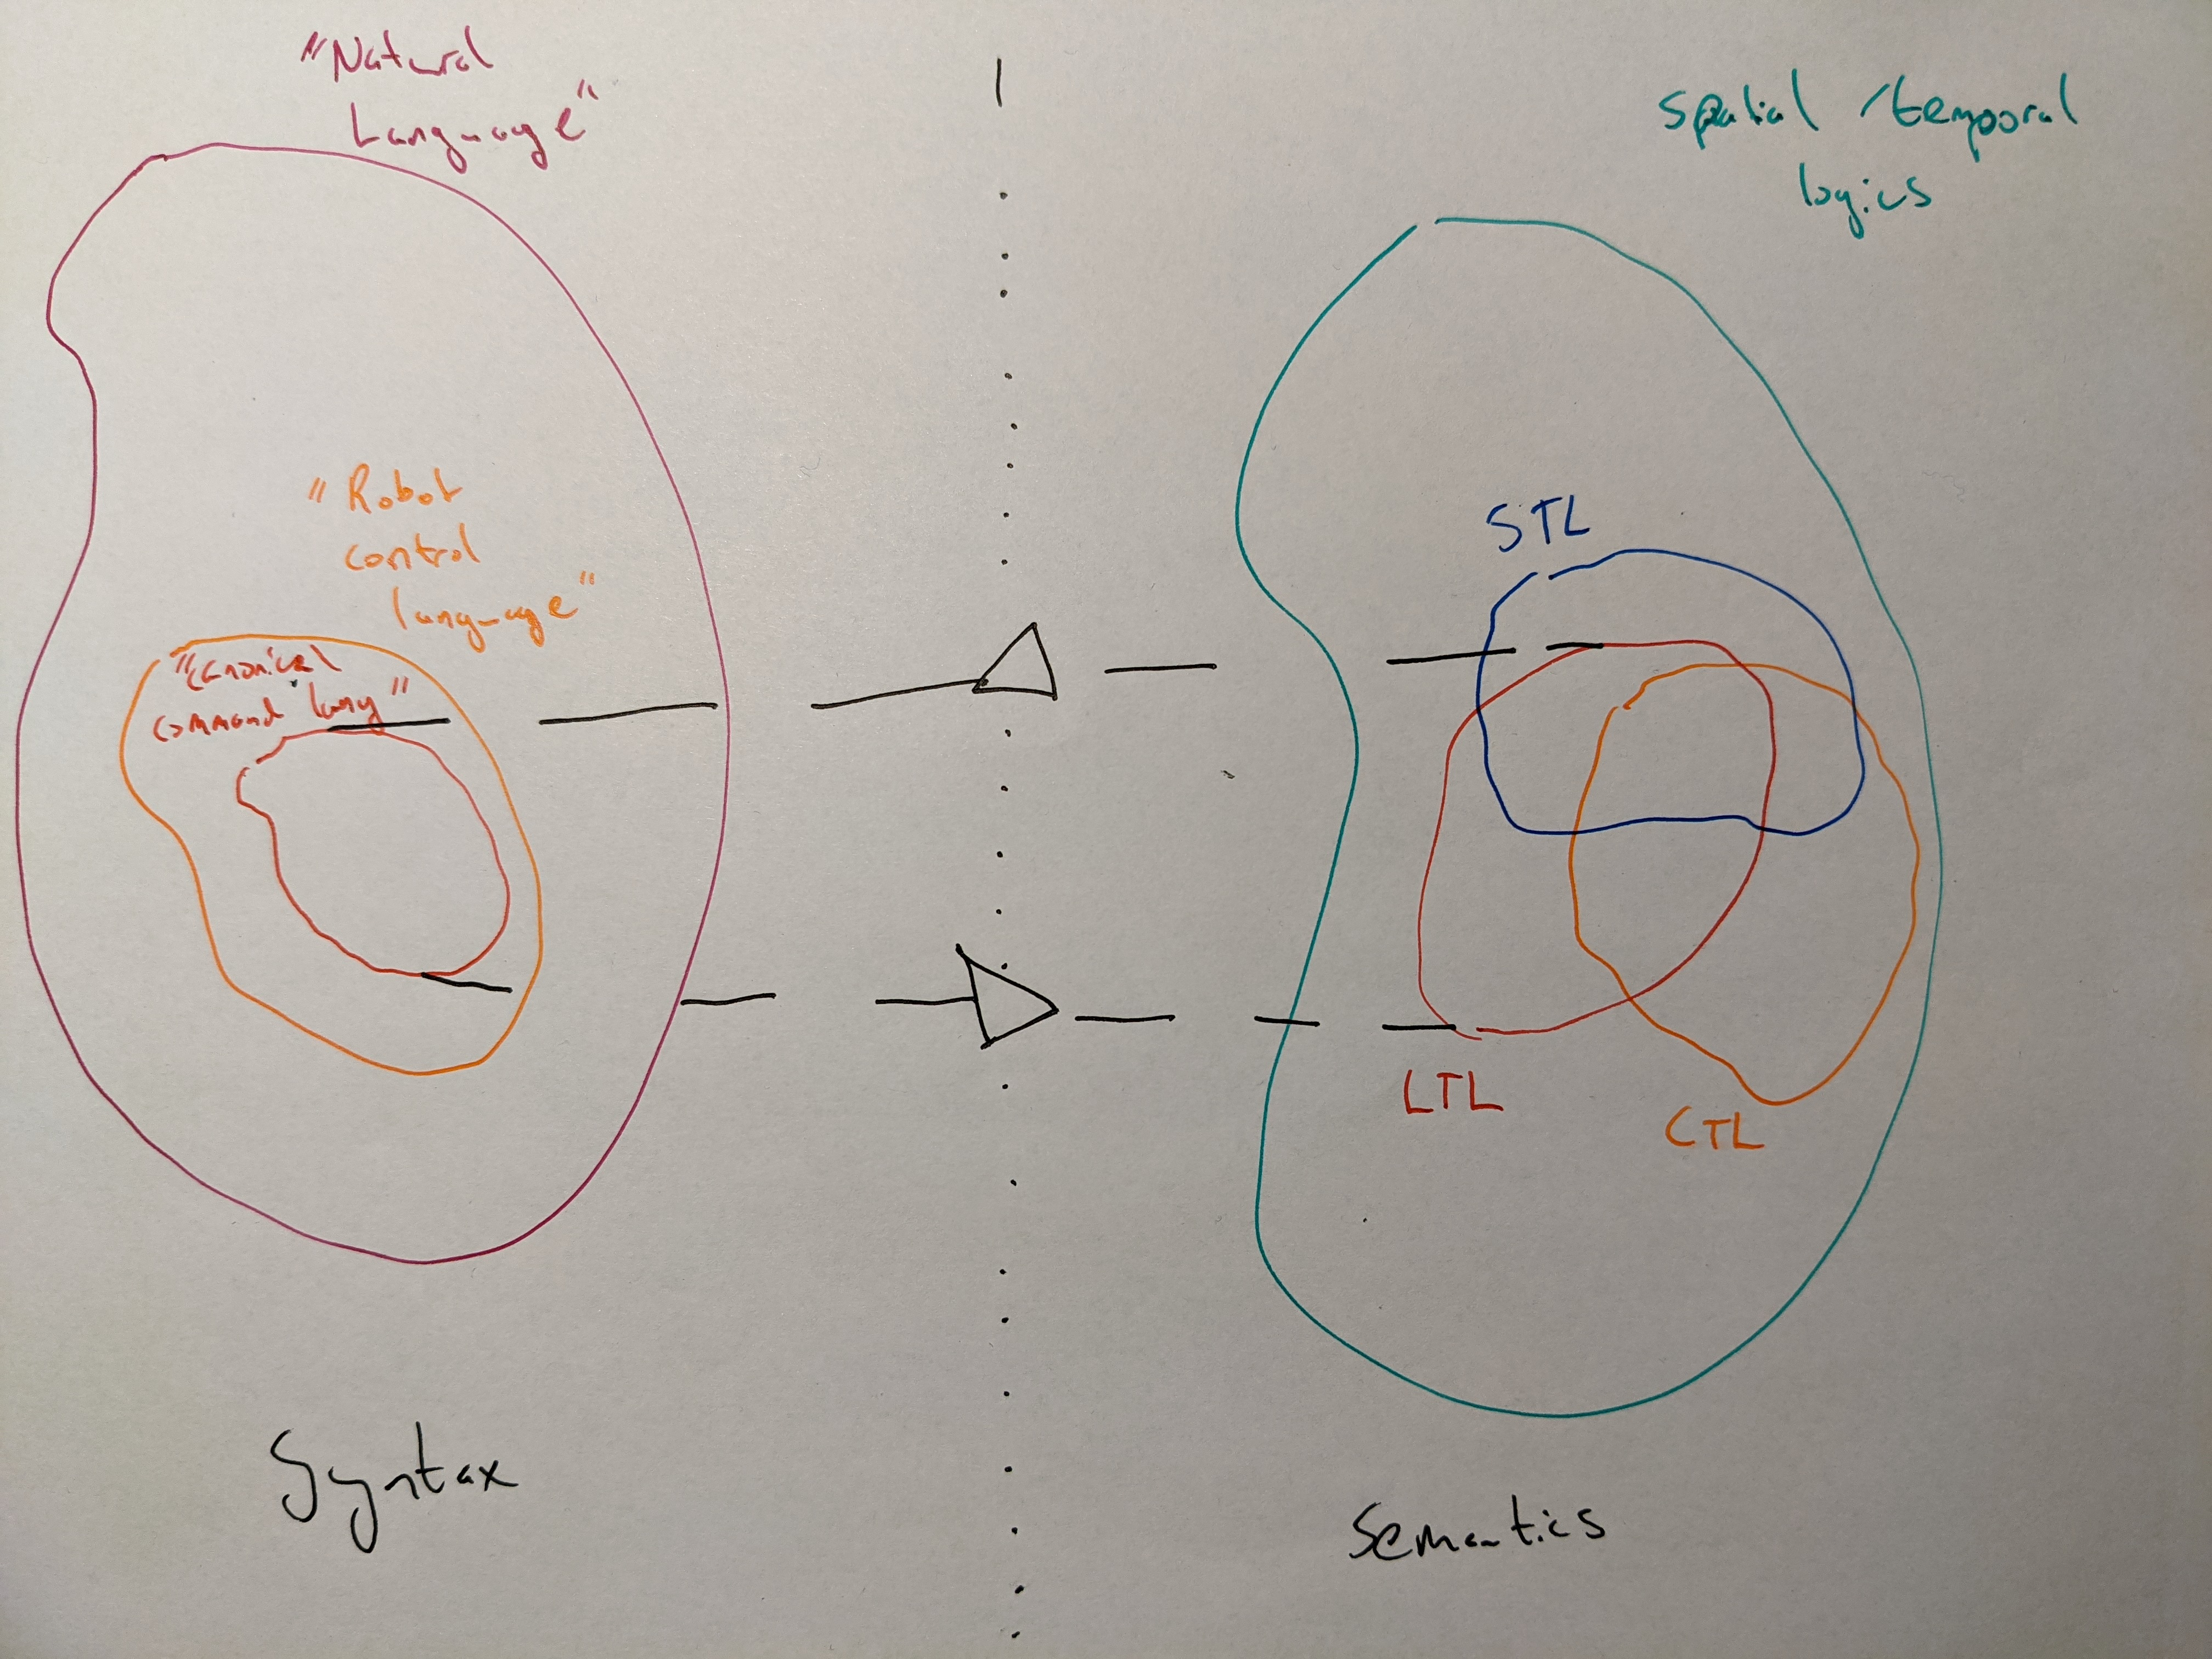
\includegraphics[width= \paperwidth]{pics/one.jpg}
\end{figure}
\end{frame}

\begin{frame}
\frametitle{Language Transformations}
\begin{figure}
\hspace*{-3mm}%
   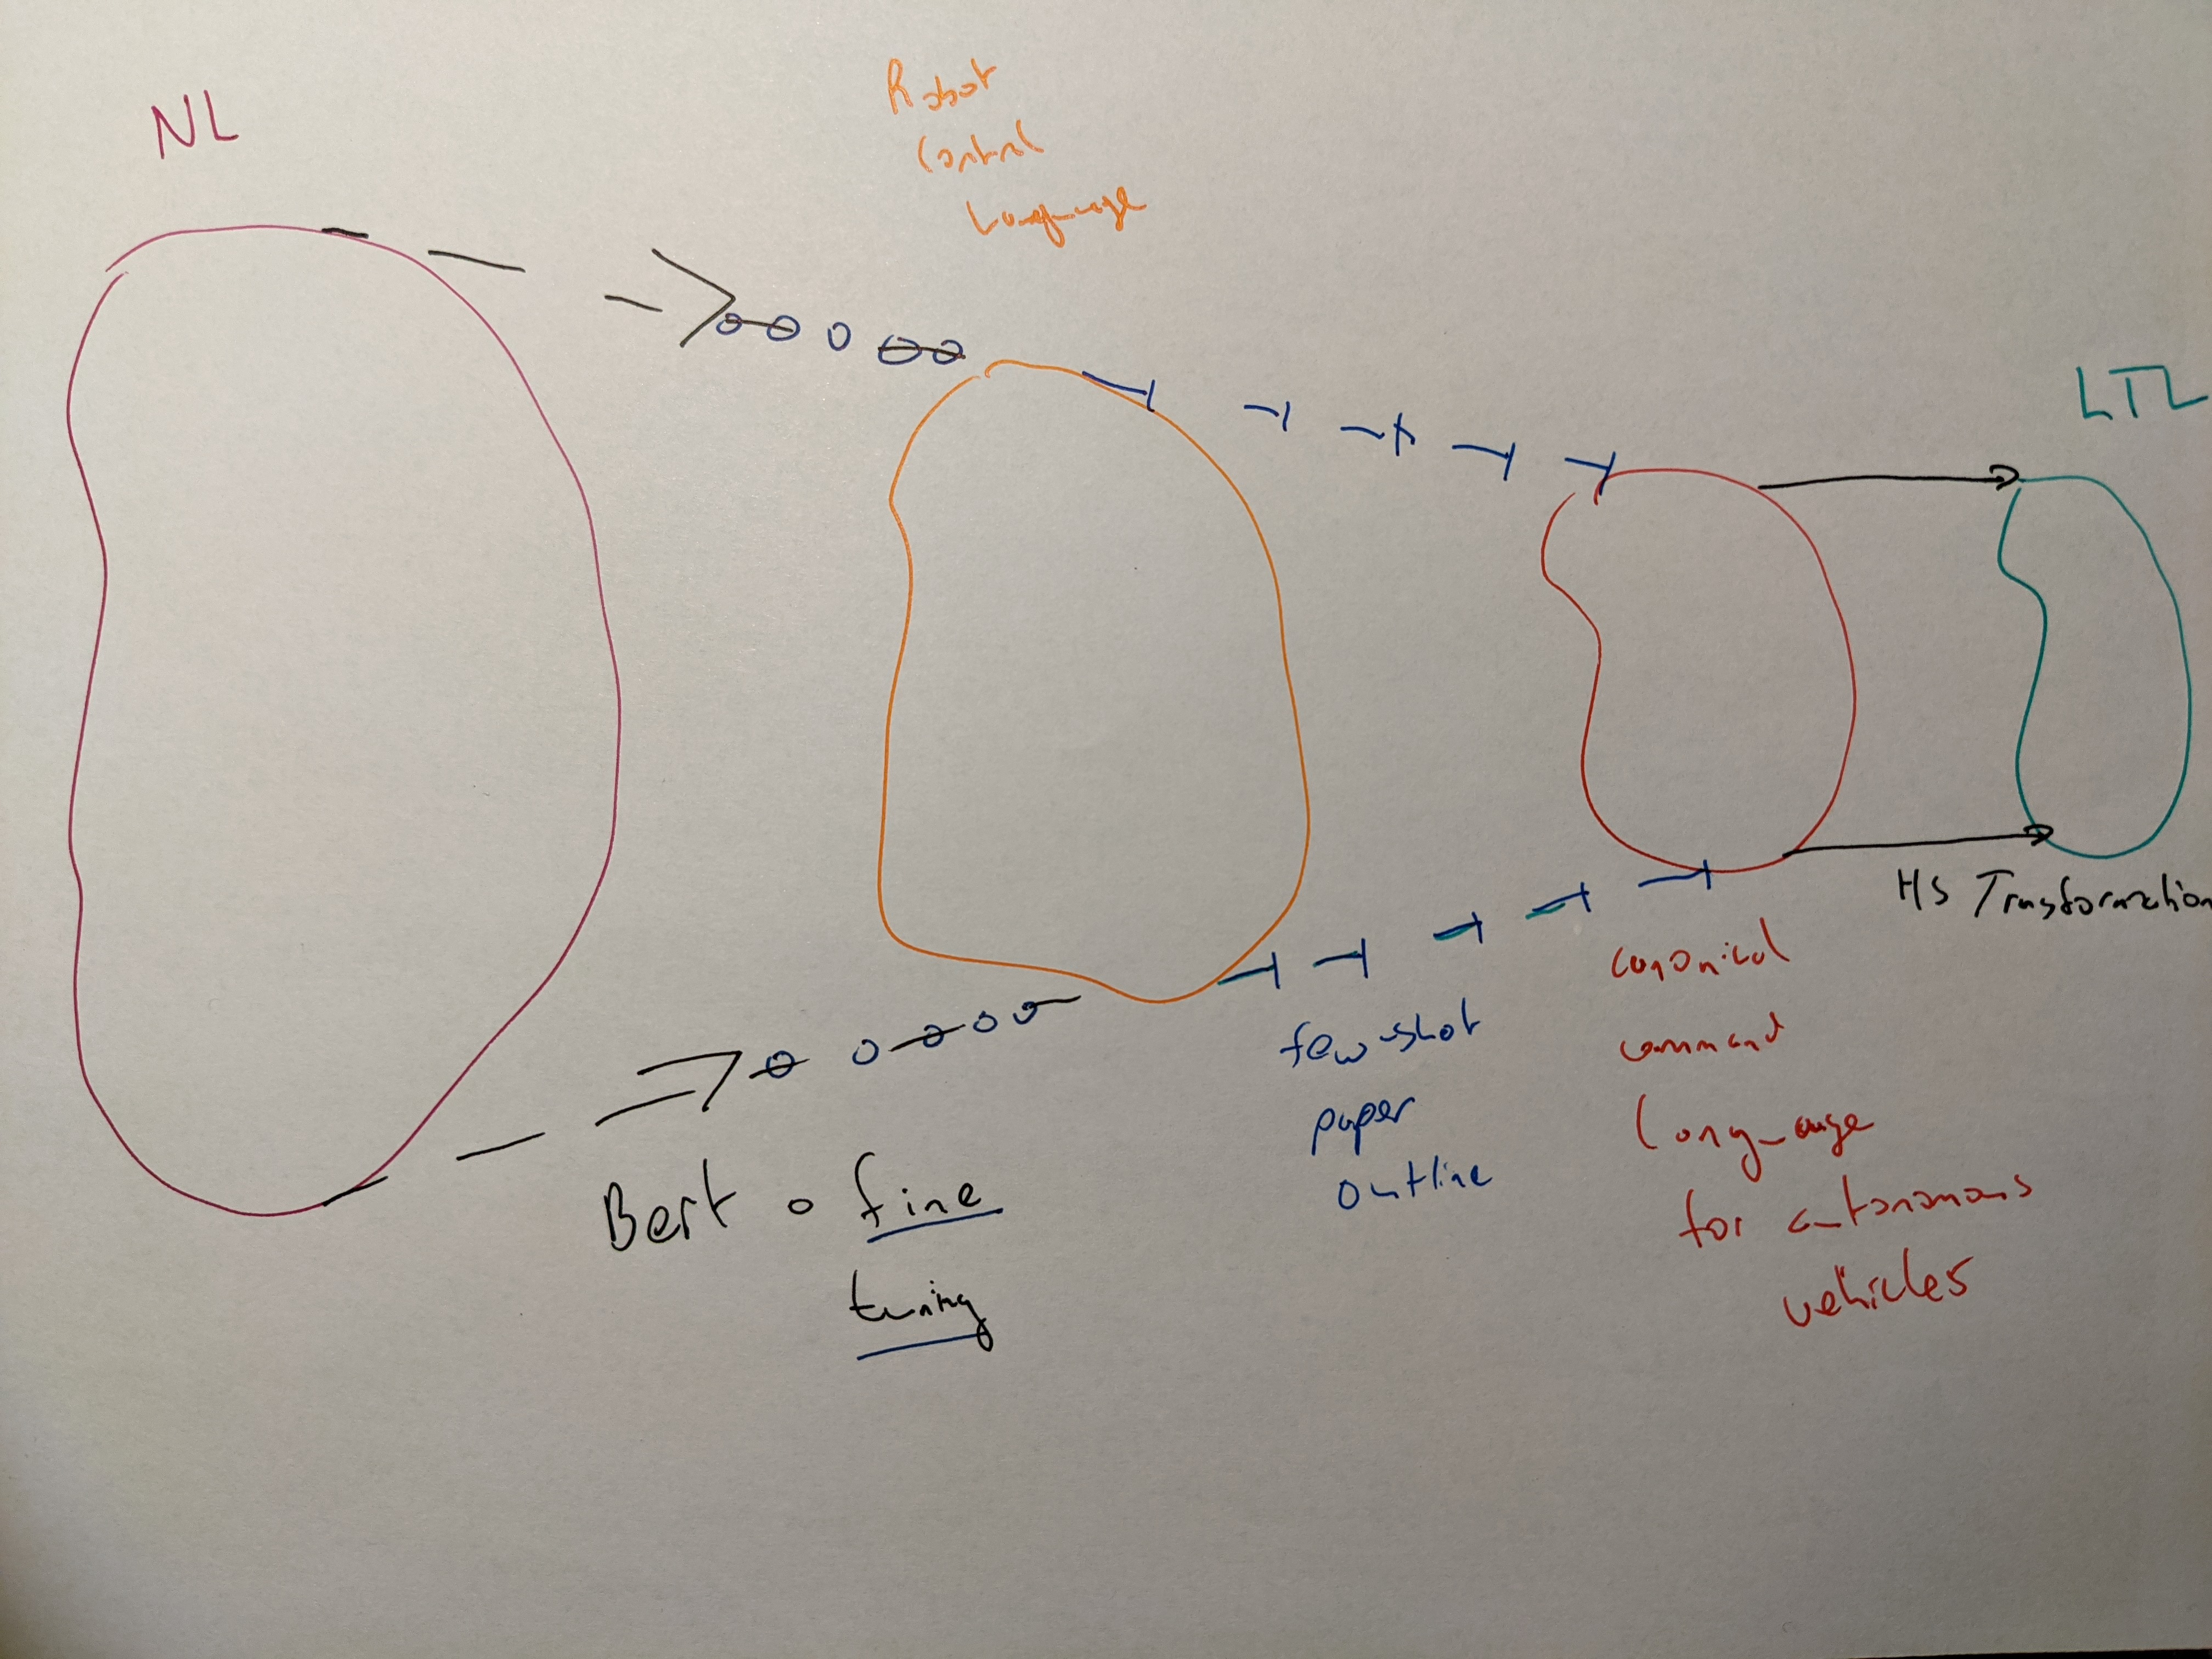
\includegraphics[width= \paperwidth]{pics/three.jpg}
\end{figure}
\end{frame}


\begin{frame}
\frametitle{Acknowledgments}
\begin{itemize}[<+->]
\item Katya
\item Matthew, Marco, Natalia, ...
\item Inari and Anka at Singapore Management University
\item Other Gothenburg People
\end{itemize}

\end{frame}

\end{document}
